% \iffalse meta-comment
%
% Copyright (C) 2017- by Yanshuo Chu <yanshuoc@gmail.com>
%
% This file may be distributed and/or modified under the
% conditions of the LaTeX Project Public License, either version 1.3a
% of this license or (at your option) any later version.
% The latest version of this license is in:
%
% http://www.latex-project.org/lppl.txt
%
% and version 1.3a or later is part of all distributions of LaTeX
% version 2004/10/01 or later.
%
% \fi
%
% \iffalse
%<*driver>
\ProvidesFile{heuthesis.dtx}[2021/05/06 3.0.15 Harbin Institute of Technology Thesis Template]
\documentclass{ltxdoc}
\usepackage{dtx-style}

\EnableCrossrefs
\CodelineIndex
\RecordChanges

\begin{document}
  \DocInput{\jobname.dtx}
\end{document}
%</driver>
% \fi
%
% \CheckSum{0}
%
% \CharacterTable
%  {Upper-case    \A\B\C\D\E\F\G\H\I\J\K\L\M\N\O\P\Q\R\S\T\U\V\W\X\Y\Z
%   Lower-case    \a\b\c\d\e\f\g\h\i\j\k\l\m\n\o\p\q\r\s\t\u\v\w\x\y\z
%   Digits        \0\1\2\3\4\5\6\7\8\9
%   Exclamation   \!     Double quote  \"     Hash (number) \#
%   Dollar        \$     Percent       \%     Ampersand     \&
%   Acute accent  \'     Left paren    \(     Right paren   \)
%   Asterisk      \*     Plus          \+     Comma         \,
%   Minus         \-     Point         \.     Solidus       \/
%   Colon         \:     Semicolon     \;     Less than     \<
%   Equals        \=     Greater than  \>     Question mark \?
%   Commercial at \@     Left bracket  \[     Backslash     \\
%   Right bracket \]     Circumflex    \^     Underscore    \_
%   Grave accent  \`     Left brace    \{     Vertical bar  \|
%   Right brace   \}     Tilde         \~}
%
% \DoNotIndex{\newenvironment,\@bsphack,\@empty,\@esphack,\sfcode}
% \DoNotIndex{\addtocounter,\label,\let,\linewidth,\newcounter}
% \DoNotIndex{\noindent,\normalfont,\par,\parskip,\phantomsection}
% \DoNotIndex{\providecommand,\ProvidesPackage,\refstepcounter}
% \DoNotIndex{\RequirePackage,\setcounter,\setlength,\string,\strut}
% \DoNotIndex{\textbackslash,\texttt,\ttfamily,\usepackage}
% \DoNotIndex{\begin,\end,\begingroup,\endgroup,\par,\\}
% \DoNotIndex{\if,\ifx,\ifdim,\ifnum,\ifcase,\else,\or,\fi}
% \DoNotIndex{\let,\def,\xdef,\edef,\newcommand,\renewcommand}
% \DoNotIndex{\expandafter,\csname,\endcsname,\relax,\protect}
% \DoNotIndex{\Huge,\huge,\LARGE,\Large,\large,\normalsize}
% \DoNotIndex{\small,\footnotesize,\scriptsize,\tiny}
% \DoNotIndex{\centering,\raggedright,\ref}
% \DoNotIndex{\c@secnumdepth,\@startsection,\@setfontsize}
% \DoNotIndex{\ ,\@plus,\@minus,\p@,\z@,\@m,\@M,\@ne,\m@ne}
% \DoNotIndex{\@@par,\DeclareOperation,\RequirePackage,\LoadClass}
% \DoNotIndex{\AtBeginDocument,\AtEndDocument}
%
% \GetFileInfo{\jobname.dtx}
%
%
% \def\indexname{索引}
% \def\glossaryname{修改记录}
% \IndexPrologue{\section{\indexname}}
% \GlossaryPrologue{\section{\glossaryname}}
%
% \title{\bfseries\color{violet}\heuthesis:哈尔滨工程大学学位论文模板}
% \author{{\fangsong 初砚硕}\\[5pt]\texttt{yanshuoc@gmail.com}}
% \date{v\fileversion\ (\filedate)}
% \maketitle\thispagestyle{empty}
% \begin{abstract}\noindent
% 该宏包为哈尔滨工程大学一校三区本、硕、博中英文毕业论文、开题和中期报告以及博后出站报
% 告模板。
% \end{abstract}
%
% \vskip2cm
% \def\abstractname{免责声明}
% \begin{abstract}
% \noindent
% \begin{enumerate}
% \item 本模板的发布遵守 \LaTeX\ Project Public License,使用前请认真阅读协议内
%   容。
% \item 本模板为作者根据\heu 教务处颁发的\UGR ,\heu 研究生院颁发的\PGR 编写而成
% ,为方便\heu 学生撰写毕业论文使用。
% \item \heu 教务处和研究生院只提供毕业论文写作指南,不提供官方模板(包括MS word
% ),也不会授权第三方模板为官方模板,所以此模板仅为写作指南的参考实现,不保证格
% 式审查老师不提意见。任何由于使用本模板而引起的论文格式审查问题均与本模板作者无
% 关。
% \item 任何个人或组织以本模板为基础进行修改、扩展而生成的新的专用模板,请严格遵
%   守 \LaTeX\ Project Public License 协议。由于违犯协议而引起的任何纠纷争端均与
%   本模板作者无关。
% \end{enumerate}
% \end{abstract}
%
%
% \clearpage
% \pagestyle{fancy}
% \begin{multicols}{2}[
%   \setlength{\columnseprule}{.4pt}
%   \setlength{\columnsep}{18pt}]
%   \tableofcontents
% \end{multicols}
% \clearpage
%
% \section{模板介绍}
% \heuthesis\ (\textbf{H}arbin\textbf{E}ngineering \textbf{U}niversity \LaTeX\
% \textbf{Thesis} Template) 是为了帮助\heu 毕业生撰写毕业论文而编写
% 的 \LaTeX\ 论文模板。
%
% 本文档将尽量完整的介绍模板的使用方法,如有不清楚之处可以参考示例文档或者根据
% 第~\ref{sec:howtoask} 节说明提问,有兴趣者都可以参与完善此手册,也非常欢迎对代
% 码的贡献。
%
% \note[注意:]{模板的作用在于减少论文写作过程中格式调整的时间。前提是遵守模板的
% 用法,否则即便用了 \heuthesis\ 也难以保证输出的论文符合学校规范。}
%
%
% \section{安装}
% \label{sec:installation}
% 未来
% \heuthesis\ 将已经包含在主要的 \TeX\ 发行版中,一般不需要安装,可以利用发行版自
% 带更新工具自动更新。阅读文档可以使用以下命令:
% \begin{shell}
% $ texdoc heuthesis
% \end{shell}
%
% 如果要使用开发版,需自己下载,\heuthesis\ 相关链接:
% \begin{itemize}
% \item github:\href{https://github.com/dustincys/heuthesis}
% {https://github.com/dustincys/heuthesis}
% \item oschina:\href{https://git.oschina.net/dustincys/heuthesis}
% {https://git.oschina.net/dustincys/heuthesis}\\ 或码云另外一个域名
% \href{https://gitee.com/dustincys/heuthesis}{https://gitee.com/dustincys/heuthesis}
% \end{itemize}
%
% \note[注意:]{如果登录不了github的同学可以登录oschina下载。}
%
% \subsection{模板的组成}
% 下表列出了 \heuthesis\ 的主要文件及其功能介绍:
%
% \begin{longtable}{l|p{8cm}}
% \toprule
% {\heiti 文件(夹)} & {\heiti 功能描述}\\\midrule
% \endfirsthead
% \midrule
% {\heiti 文件(夹)} & {\heiti 功能描述}\\\midrule
% \endhead
% \endfoot
% \endlastfoot
% heuthesis.ins & \textsc{DocStrip} 驱动文件(开发用) \\
% heuthesis.dtx & \textsc{DocStrip} 源文件(开发用)\\\midrule
% heuthesisbook.cls & 模板类文件\\
% heuthesisbook.cfg & 模板配置文件\\
% heuthesis.bst & 参考文献样式文件\\\midrule
% heuthesis.ist & 索引样式文件\\\midrule
% reference.bib & 文档参考文献\\
% main.tex & 示例文档主文件\\
% front/ & 正文之前内容\\
% body/ & 正文内容\\
% body/ & 正文之后内容\\
% figures/ & 示例文档图片路径\\
% heuthesis.sty & 为示例文档加载其它宏包\\\midrule
% Makefile & Makefile\\
% latexmkrc & latexmk 配置文件 \\
% README.md & Readme\\
% \textbf{heuthesis.pdf} & 用户手册(本文档)\\\bottomrule
% \end{longtable}
%
% 几点说明:
% \begin{itemize}
% \item \file{heuthesisbook.cls} 和 \file{heuthesisbook.cfg} 可由 \file{heuthesis.ins}
%   和 \file{heuthesis.dtx} 生成。
% \item 使用前阅读文档:\file{heuthesis.pdf}。
% \item 默认的生成的论文中含有丰富的格式示例,使用前请仔细阅读\file{main.pdf}。
% \end{itemize}
%
% \subsection{生成模板}
% \label{sec:generate-cls}
% \note[提示:]{若使用 \TeX 发行版自带的 \heuthesis\ 或 Github/OSChina
% 上发布的版本,可忽略此节,直接阅读第~\ref{sec:generate-thesis}节。若下载
% CTAN 包或者 Github/OSChina 开发代码,请阅读本节了解生成模板文件的步骤。}
%
% 模板解压缩后生成文件夹 \file{heuthesis-vX.Y.Z}\footnote{\texttt{vX.Y.Z} 为版本号。},
% 其中包括:模板源文件(\file{heuthesis.ins} 和 \file{heuthesis.dtx}),参考文献
% 样式 \file{heuthesis.bst},示例文档
% (\file{main.tex},\file{shuji.tex},\file{heuthesis.sty}\footnote{可能用到的包
% 以及一些命令定义都放在这里,以免 \file{heuthesisbook.cls} 过分臃
% 肿。},\file{data/} 和 \file{figures/} 和 \file{ref/})。在使用之前需要先生成模
% 板文件和配置文件(具体命令细节请参考 \file{README.md} 和 \file{Makefile}):
%
% \begin{shell}
% $ cd heuthesis-vX.Y.Z
% # 生成 heuthesisbook.cls 和 heuthesisbook.cfg
% $ latex heuthesis.ins
%
% # 下面的命令用来生成用户手册,可以不执行
% $ xelatex heuthesis.dtx
% $ makeindex -s gind.ist -o heuthesis.ind heuthesis.idx
% $ makeindex -s gglo.ist -o heuthesis.gls heuthesis.glo
% $ xelatex heuthesis.dtx
% $ xelatex heuthesis.dtx  % 生成说明文档 heuthesis.pdf
% \end{shell}
%
% \subsection{生成论文}
% \label{sec:generate-thesis}
% 本节介绍几种常见的生成论文的方法。用户可根据自己的情况选择。
%
% \subsubsection{\XeLaTeX}
% \label{sec:xelatex}
% 很多用户对 \LaTeX\ 命令执行的次数不太清楚。一个基本的原则是多次运行 \LaTeX\ 命
% 令直至不再出现警告。下面给出生成示例文档的详细过程(\texttt{\#} 开头的行为注
% 释),首先来看推荐的 \texttt{xelatex} 方式:
% \begin{shell}
% # 1. 发现里面的引用关系,文件后缀 .tex 可以省略
% $ xelatex main
%
% # 2. 编译参考文件源文件,生成 bbl 文件
% $ bibtex main
%
% # 3. 下面解决引用
% $ xelatex main
% $ xelatex main   # 如果不需要生成索引此时生成完整的 pdf 文件
% $ splitindex main -- -s heuthesis.ist  # 自动生成索引
% $ xelatex main.tex
% \end{shell}
%
% \subsubsection{latexmk}
% \label{sec:latexmk}
% \texttt{latexmk} 命令支持全自动生成 \LaTeX\ 编写的文档,并且支持使用不同的工具
% 链来进行生成,它会自动运行多次工具直到交叉引用都被解决。下面给出了一个用
% \texttt{latexmk} 调用 \texttt{xelatex} 生成最终文档的示例:
% \begin{shell}
% # 一句话就够了!
% $ latexmk -xelatex main
% \end{shell}
%
% \subsubsection{make}
% \label{sec:make}
% \note[提示:]{若要使用 \texttt{make} 编译,需自行下载模板。因为 \TeX\ 发行版中
% 的 \file{Makefile} 不在当前目录。}
%
% 上面的方法虽然不复杂,但是每次都输入还是非常罗嗦,所以 \heuthesis\ 提供了一
% 个 \file{Makefile}:
%
% \begin{shell}
% $ make clean
% $ make cls       # 生成 heuthesisbook.cls 和 heuthesisbook.cfg
% $ make doc       # 生成说明文档 heuthesis.pdf
% $ make thesis    # 生成示例文档 main.pdf
% \end{shell}
%
% \heuthesis\ 的 \file{Makefile} 默认用 \texttt{latexmk} 调用\texttt{xelatex} 编
% 译,此外还支持直接用 \texttt{xelatex} 编译。如有需要可修
% 改 \file{Makefile} 开头的参数或通过命令行传递参数(请参看 \file{README.md}),
% 进一步还可以修改 \file{latexmkrc} 进行定制。
%
% \subsection{升级}
% \label{sec:updgrade}
% \heuthesis\ 升级非常简单,可以通过 \TeX 发行版的包管理工具自动更新发行版,也可
% 以下载最新的开发版,
% 将 \file{heuthesis.ins},\file{heuthesis.dtx} 拷贝至工作目
% 录覆盖相应的文件,然后运行:
% \begin{shell}
% $ latex heuthesis.ins
% \end{shell}
%
% 生成新的类文件和配置文件即可。也可以直接拷
% 贝 \file{heuthesisbook.cls},\file{heuthesisbook.cfg} 和
% \file{heuthesis.ist},免去上面命令的执行。
%
%
% \section{使用说明}
% \label{sec:usage}
% 本手册假定用户已经能处理一般的 \LaTeX\ 文档,并对 \BibTeX\ 有一定了解。如果
% 从来没有接触过 \TeX\ 和 \LaTeX,建议先学习相关的基础知识。
%
% \subsection{关于提问}
% \label{sec:howtoask}
% 按照优先级推荐提问的位置如下:
%
% \begin{itemize}
% \item \href{http://github.com/dustincys/heuthesis/issues}{Github Issues}
% \item \href{https://git.oschina.net/dustincys/heuthesis/issues}{OSChina Issues}
% \item heuthesis QQ 讨论群:259959600
% \end{itemize}
%
% \subsection{示例文件}
% \label{sec:userguide}
% 模板核心文件有三
% 个:\file{heuthesisbook.cls},\file{heuthesisbook.cfg} 和\file{heuthesis.bst},但是如果
% 没有示例文档用户会发现很难下手。所以推荐新用户从模板自带的示例文档入手,里面包
% 括了论文写作用到的所有命令及其使用方法,只需要用自己的内容进行相应替换就可以。
% 对于不清楚的命令可以查阅本手册。下面的例子描述了模板中章节的组织形式,来自于示
% 例文档,具体内容可以参考模板附带的 \file{main.tex}。
%
% \lstinputlisting[style=lstStyleLaTeX]{examples/book/english/thesis.tex}
% \lstinputlisting[style=lstStyleLaTeX]{examples/book/chinese/thesis.tex}
% \lstinputlisting[style=lstStyleLaTeX]{examples/art/reports/report.tex}
% \lstinputlisting[style=lstStyleLaTeX]{examples/art/reportplus/report.tex}
%
% \subsection{论文选项}
% \label{sec:option}
%
% 论文选项,就是在\file{main.tex}文件的开头,非注释的第一行的方括号中填写的选项,示例见上节。
% 各个选项的含义说明已经在上节中说明,所以这里就不重复了。
%
% \subsection{中文字体}
% \label{sec:chinese-fonts}
% 正确配置中文字体是使用模板的第一步。模板调用 \CTeX\ 宏包,只提供基于
% \pkg{xeCJK} 包,使用 \XeLaTeX\ 编译的方式。
% 关于如何使用字体命令、字号等等,属于模板格式范畴,在实现细节中讨论。
% 关于中文字体安装、配置的所有问题不在本模板讨论 范围。
%
% \subsection{前文}
% \label{sec:titlepage}
% 前文内容是正文之前,含封面、摘要、目录、符号表。
% 封面信息提供两种配置方法:一是通过统一设置命 令 \cs{heusetup}
% 通过\emph{key=value} 形式完成;二是每个信息利用命令独立设置, 其中命令的名字跟
% \emph{key} 相同。两种方式可以交叉使用,并按顺序执行(即后来的设置会覆
% 盖前面的)。以 \texttt{c} 开头的命令跟中文相关,\texttt{e}
% 开头则为对应的英文。
%
% \DescribeMacro{\heusetup}
% \cs{heusetup} 用法与常见 \emph{key=value} 命令相同,如下:
% \begin{latex}
% \heusetup{
%   key1 = value1,
%   key2 = {a value, with comma},
% }
% % 可以多次调用
% \heusetup{
%   key3 = value3,
%   key1 = value11, % 覆盖 value1
% }
% \end{latex}
%
% \note[注意:]{\cs{heusetup} 使用 \pkg{kvoptions} 机制,所以配置项之间不能有空行,否则
% 会报错。}
%
% 大多数命令的使用方法都是: \cs{command}\marg{arg},例外者将具体指出。这些命令都
% 在示例文档的 \file{front/cover.tex} 中。
%
% \subsubsection{密级}
% \label{sec:setup-secret}
% \DescribeMacro{statesecrets}
% \DescribeMacro{natclassifiedindex}
% \DescribeMacro{intclassifiedindex}
% 定义秘密级别和国内国际索引号。
% \begin{latex}
% \heusetup{
% statesecrets={公开},
% natclassifiedindex={TM301.2},
% intclassifiedindex={62-5},
% }
% \end{latex}
%
% \subsubsection{论文标题}
% \myentry{论文标题}
% \DescribeMacro{ctitle}
% \DescribeMacro{etitle}
% \DescribeMacro{ctitleone}
% \DescribeMacro{ctitletwo}
% \DescribeMacro{csubtitle}
% \DescribeMacro{esubtitle}
% 中英文标题。
% 如果有副标题,需要在封面选项中设置subtitle=true,否则不显示副标题。
% \begin{latex}
% \heusetup{
%   ctitlecover={封面中文题目可断行},
%   ctitle={论文中文题目},
%   etitle={Thesis English Title},
%   csubtitle={论文中文副题目(如果有)},
%   esubtitle={Thesis English Sub-Title (if necessary)},
%   ctitleone={本科生论文中文题目上部分},
%   ctitletwo={本科生论文中文题目下部分},
% }
% \end{latex}
%
% \subsubsection{作者姓名}
% \myentry{作者姓名}
% \DescribeMacro{cauthor}
% \DescribeMacro{eauthor}
% 作者姓名。
% \begin{latex}
% \heusetup{
%   cauthor={中文姓名},
%   eauthor={Name in Pinyin}
% }
% \end{latex}
%
% \subsubsection{申请学位名称}
% \label{sec:degree}
% \myentry{学科名称}
% \DescribeMacro{cxueke}
% \DescribeMacro{exueke}
% 按照入学的培养计划中学科自行填写,具体学科名称不是本文档范畴。
%
% \begin{latex}
% \heusetup{
%   cxueke={工学},
%   exueke={Engineering},
% }
% \end{latex}
%
% \subsubsection{院系名称}
% \myentry{院系名称}
% \DescribeMacro{caffil}
% \DescribeMacro{eaffil}
% 院系名称,同上,按照入学的培养计划中学科自行填写,具体院系名称不是本文档范畴。
% \begin{latex}
% \heusetup{
%  caffil={机电工程学院},
%  eaffil={\emultiline[t]{School of Mechatronics Engineering \\ Mechatronics Engineering}},
% }
% \end{latex}
% \note[注意:]{个别学院英文名过长,使用以上方法自行换行。}
%
% \subsubsection{专业名称}
% \myentry{专业名称}
% \DescribeMacro{csubject}
% \DescribeMacro{esubject}
% 专业名称,同上,按照入学的培养计划中学科自行填写,具体名称不是本文档范畴。
% \begin{latex}
% \heusetup{
%  csubject={机械制造及其自动化},
%  esubject={Computer Science and Technology},
% }
% \end{latex}
%
% \subsubsection{导师}
% \myentry{导师}
% \DescribeMacro{csupervisor}
% \DescribeMacro{esupervisor}
% 直接导师。
% \begin{latex}
% \heusetup{
%   csupervisor={导师~教授},
%   esupervisor={Supervisor}
% }
% \end{latex}
%
% \myentry{副导师}
% \DescribeMacro{cassosupervisor}
% \DescribeMacro{eassosupervisor}
% 副指导教师。
% \begin{latex}
% \heusetup{
%   cassosupervisor={副导师~副教授},
%   eassosupervisor={2nd Boss}
% }
% \end{latex}
%
% \myentry{联合导师}
% \DescribeMacro{ccosupervisor}
% \DescribeMacro{ecosupervisor}
% 硕士生联合指导教师,博士生联合导师。
% \begin{latex}
% \heusetup{
%   ccosupervisor={联合导师~教授},
%   ecosupervisor={3rd Boss}
% }
% \end{latex}
%
% \subsubsection{成文日期}
% \myentry{日期}
% \DescribeMacro{cdate}
% \DescribeMacro{edate}
% 默认为当前时间,也可以自己指定。
% \begin{latex}
% \heusetup{
%   cdate={中文日期},
%   edate={English Date},
% }
% \end{latex}
%
% \subsubsection{学生类型}
% \myentry{学生类型}
% \DescribeMacro{cstudenttype}
% \DescribeMacro{estudenttype}
% 非全日制教育申请学位者
%(同等学力人员)、(工程硕士)、(工商管理硕士)、
%(高级管理人员工商管理硕士)、(公共管理硕士)、(中职教师)、(高校教师)等,
% 具体要求按照入学的培养计划中学科自行填写,具体名称不是本文档范畴。
% \begin{latex}
% \heusetup{
%   cstudenttype={同等学力人员},
%   estudenttype={Master of Art},
% }
% \end{latex}
%
% \subsubsection{学号}
% \myentry{学号}
% \DescribeMacro{cstudentid}
% 学号,具体要求按照入学的培养计划中学科自行填写。
% \begin{latex}
% \heusetup{
%   cstudentid={9527},
% }
% \end{latex}
%
% \subsubsection{摘要}
% \myentry{摘要正文}
% \DescribeEnv{cabstract}
% \DescribeEnv{eabstract}
% \note[说明:]{摘要正文只能用环境命令的形式,不支持 \cs{heusetup}。}
%
% \begin{latex}
% \begin{cabstract}
%  摘要请写在这里...
% \end{cabstract}
%
% \begin{eabstract}
%  Here comes the abstract in English...
% \end{eabstract}
% \end{latex}
%
% \myentry{关键词}
% \DescribeMacro{ckeywords}
% \DescribeMacro{ekeywords}
% 关键词用英文逗号分割写入相应的命令中,模板会解析各关键词并生成符合不同论文格式
% 要求的关键词格式。
% \begin{latex}
% \heusetup{
%   ckeywords={关键词 1, 关键词 2},
%   ekeywords={keyword 1, keyword 2}
% }
% \end{latex}
%
% \subsubsection{符号对照表}
% \DescribeEnv{denotation}
% 主要符号表环境,单独在文件\file{front/denotation.tex}中。
% 跟据\PGR\
% 示例中要求,我工符号表是table环境,示例文件如下,由于我工要求博士论文图表标题是双语,所以任何对单个标题的全局格式调整都会影响到双语标题,所以这里使用\cs{vspace},具体见实现细节中的描述。
% \begin{latex}
% \begin{denotation}
% \begin{table}[h]%此处最好是h
% \caption{国际单位制中具有专门名称的导出单位}
% \vspace{0.5em}\centering\wuhao
% \begin{tabular}{ccccc}
% \toprule[1.5pt]
% 量的名称&单位名称&单位符号&其它表示实例\\
% \midrule[1pt]
% 频率&赫[兹]&Hz&s-1\\
% \bottomrule[1.5pt]
% \end{tabular}
% \end{table}
% \end{denotation}
% \end{latex}
%
% \subsubsection{目录}
% 目录不需要用户干预,自动生成,具体命令已经写在\file{main.tex}中。
%
% \subsection{正文}
%
% \subsubsection{图和表}
% \heu\ 博士毕业论文要求使用中英双语图题、表题,这增加了维护难度。
% 因为现有唯一的方法是在已有的图题或表题的基础上再添加一行英语图题或表题。
% 两个题之间的距离具体多少不在\PGR\ 中要求。目前的方法是用户手动调节该距离。
% 关于图题\PGR\ 和\UGR\ 只规定了居中,并没有规定居中对其。然而评审老师很多喜欢居
% 中且居中对齐。模板默认选项是居中且居中对齐,如果不喜欢居中对齐,那么需要在
% \file{main.tex}的文档类选项中设置选项capcenterlast=false。详细方法见前文的介绍
% 。
% \begin{heurgu}
% 每个图均应有图题(由图序和图名组成),图题不宜有标点符号,图名在图序之后空1个
% 半角字符排写。图序按章编排,如第1章第一个插图的图号为“图1-1”。图题置于图下,硕
% 士论文只用中文,博士论文用中、英两种文字,居中书写,中文在上,要求中文用宋体5
% 号字,英文用Times New Roman 5号字。有图注或其它说明时应置于图题之上。引用图应
% 注明出处,在图题右上角加引用文献号。图中若有分图时,分图题置于分图之下或图题之
% 下,可以只用中文书写,分图号用a)、b)等表示。图中各部分说明应采用中文(引用的外
% 文图除外)或数字符号,各项文字说明置于图题之上(有分图时,置于分图题之上)。图
% 中文字用宋体、Times New Roman字体,字号尽量采用5号字(当字数较多时可用小5号字
% ,以清晰表达为原则,但在一个插图内字号要统一)。同一图内使用文字应统一。图表中
% 物理量、符号用斜体。
% \end{heurgu}
% 单双语图题的方法如下,注释中说明。
% \begin{latex}
% \begin{figure}[htpb]
% \centering
% 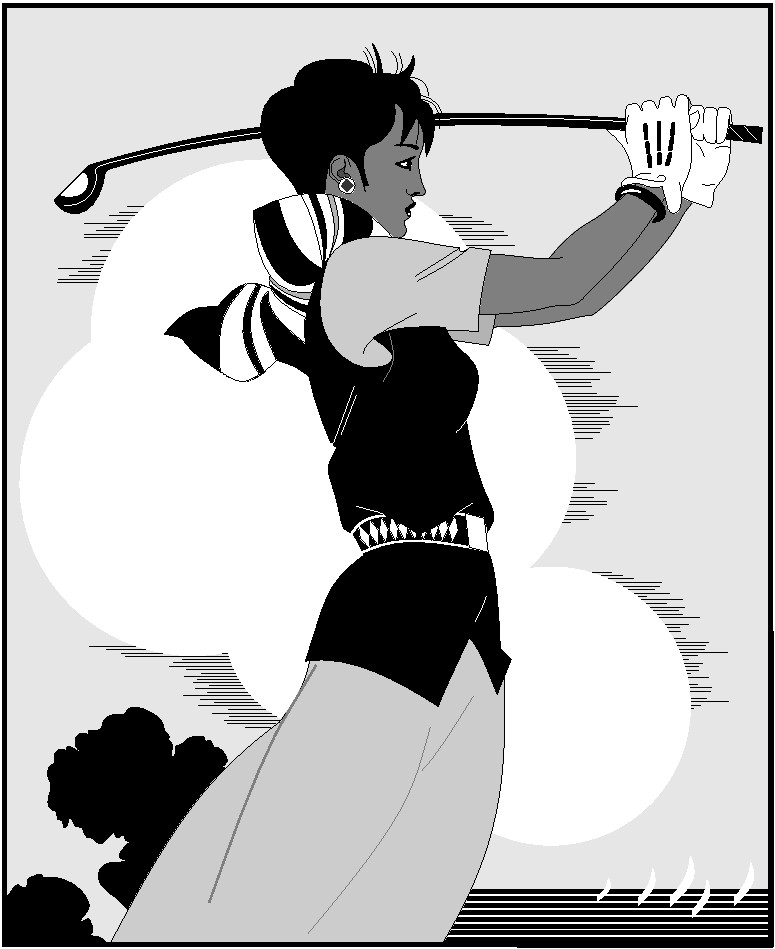
\includegraphics[width = 0.4\textwidth]{golfer}
% \bicaption[golfer1]{}{注意图中文字尽量用五号字
% }{Fig.$\!$}{The person playing golf}
% \end{figure}
% \end{latex}
% 单张单图题的格式如下,
% \begin{latex}
% \begin{figure}[h]
% \centering
% 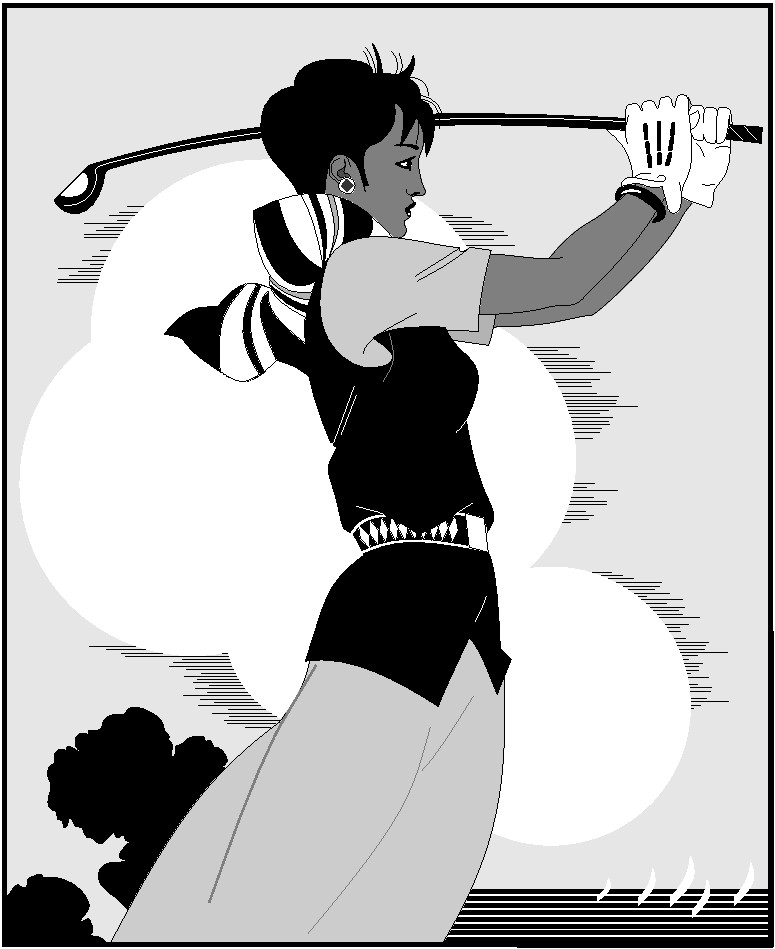
\includegraphics[width = 0.4\textwidth]{golfer}
% \caption{注意图中文字字号尽量用五号字}
% \end{figure}
% \end{latex}
% 并排图例。
% \begin{latex}
% \begin{figure}[htbp]
% \centering
% \begin{minipage}{0.4\textwidth}
% \centering
% 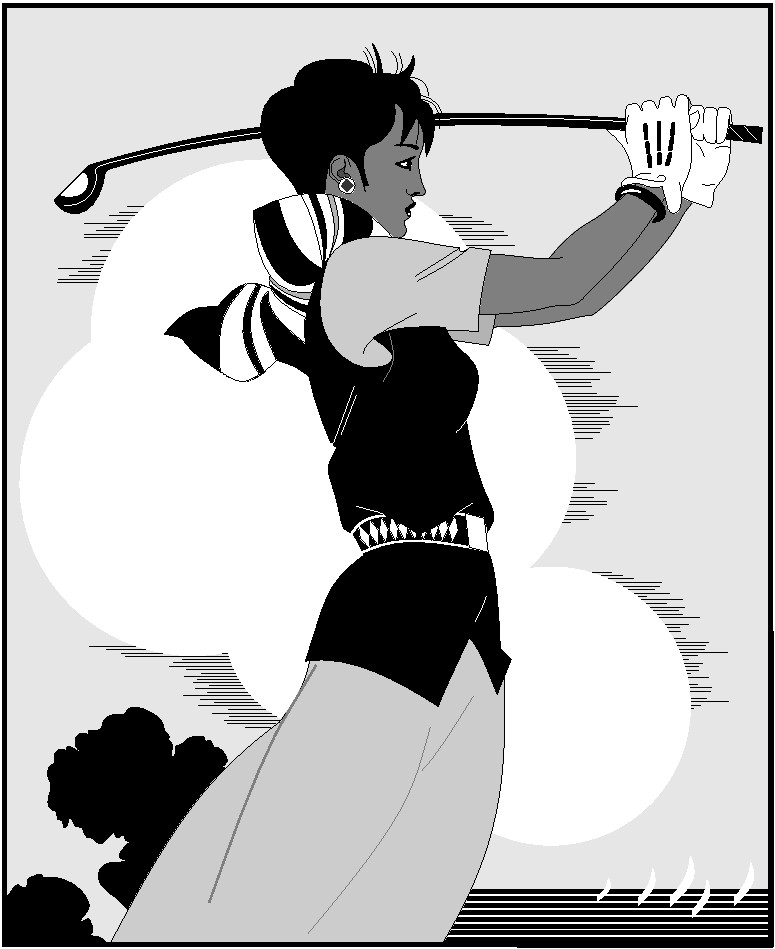
\includegraphics[width=\textwidth]{golfer}
% \bicaption[golfer2]{}{打高尔夫球的人}{Fig.$\!$}{The person playing golf}
% \end{minipage}
% \begin{minipage}{0.4\textwidth}
% \centering
% 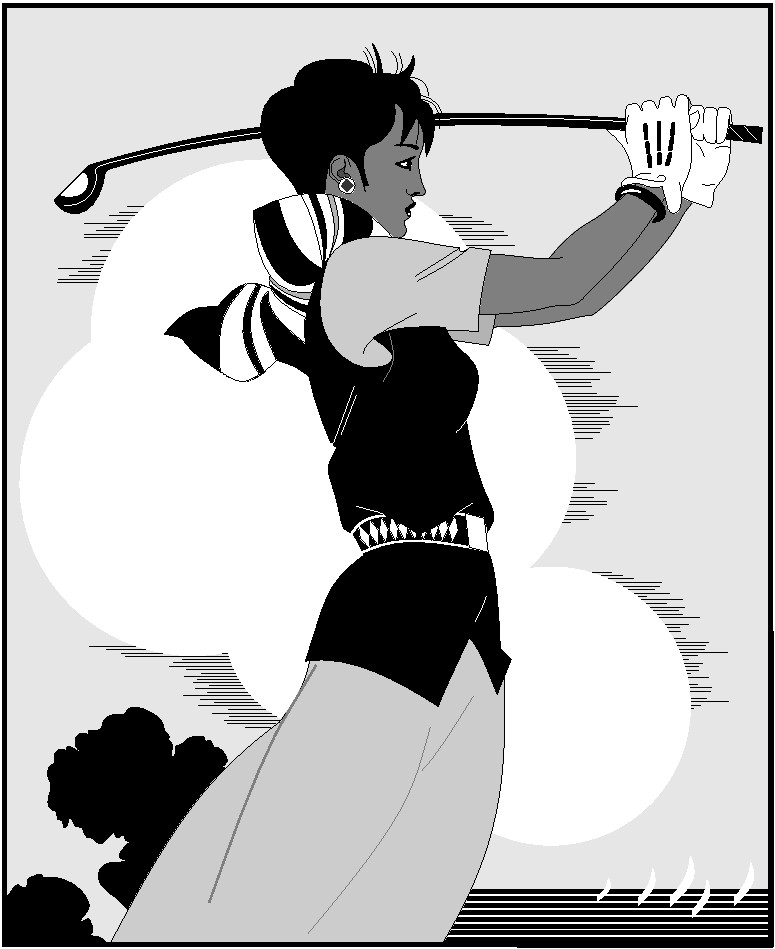
\includegraphics[width=\textwidth]{golfer}
% \bicaption[golfer3]{}{打高尔夫球的人}{Fig.$\!$}{The person playing golf}
% \end{minipage}
% \end{figure}
% \end{latex}
% 子图图例。
% \begin{latex}
% \begin{figure}[htbp]
% \centering
% \subfigure{\label{golfer41}}\addtocounter{subfigure}{-2}
% \subfigure[The person playing golf]{\subfigure[打高尔夫球的人~1]{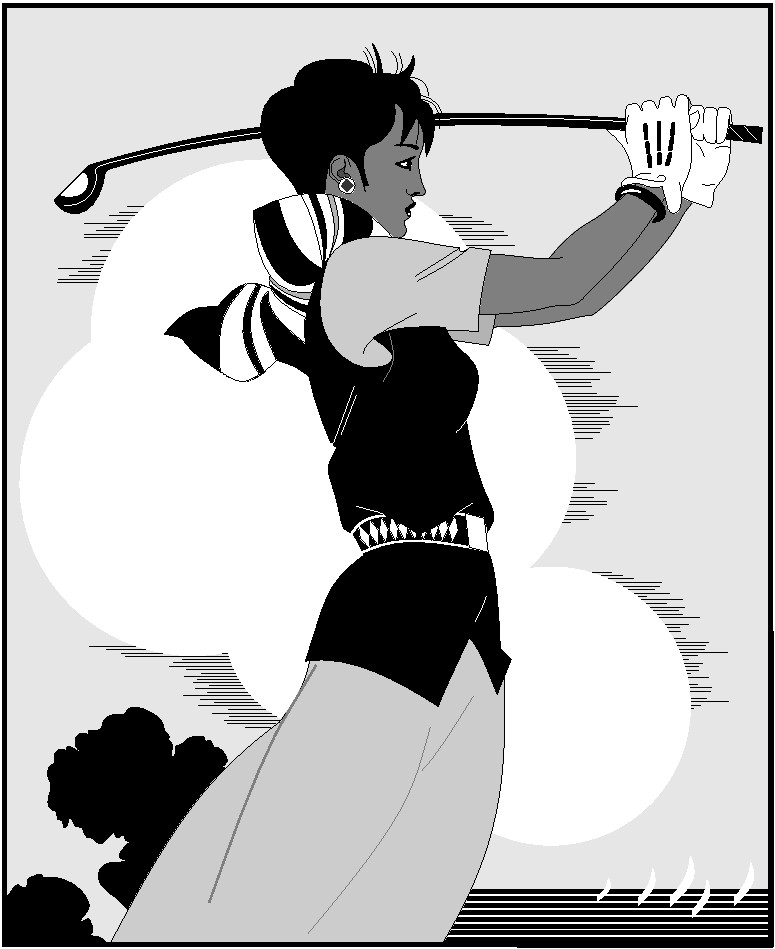
\includegraphics[width=0.4\textwidth]{golfer}}}
% \subfigure{\label{golfer42}}\addtocounter{subfigure}{-2}
% \subfigure[The person playing golf]{\subfigure[打高尔夫球的人~2]{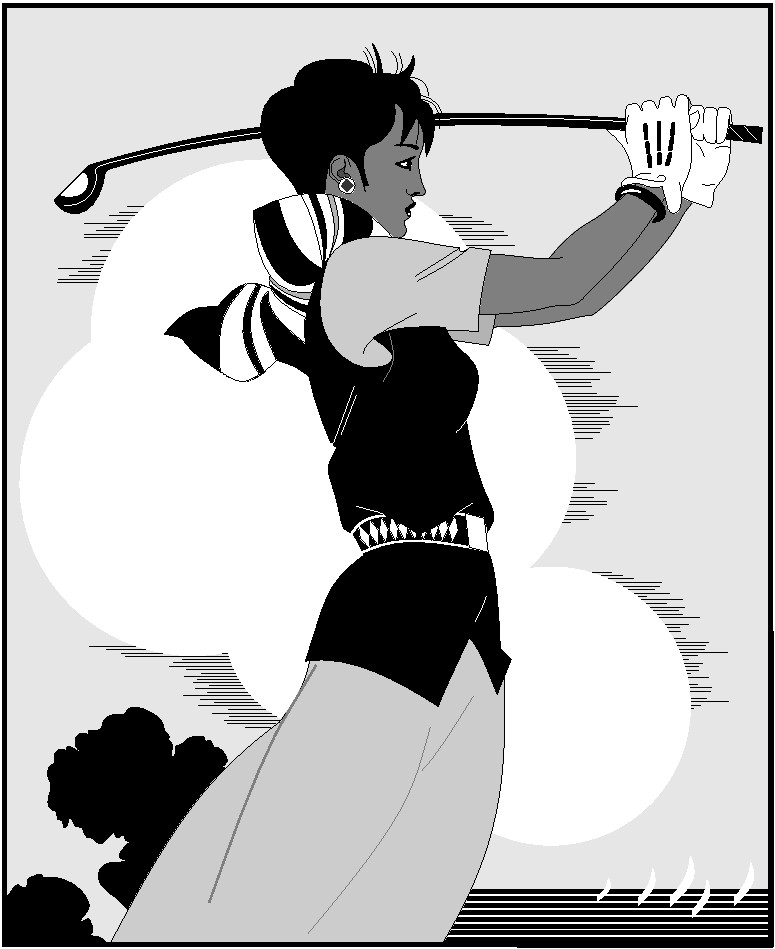
\includegraphics[width=0.4\textwidth]{golfer}}}
% \bicaption[golfer4]{}{打高尔夫球的人}{Fig.$\!$}{The person playing golf}
% \end{figure}
% \end{latex}
% 表格示例,表格中的字体是可以自行调整的。
% \begin{latex}
% \begin{table}[htbp]
% \bicaption[table1]{}{符合研究生院绘图规范的表格}{Table$\!$}{Table in agreement of the standard from graduate school}
% \vspace{0.5em}\centering\wuhao
% \begin{tabular}{ccccc}
% \toprule[1.5pt]
% $D$(in) & $P_u$(lbs) & $u_u$(in) & $\beta$ & $G_f$(psi.in)\\
% \midrule[1pt]
%  5 & 269.8 & 0.000674 & 1.79 & 0.04089\\
% 10 & 421.0 & 0.001035 & 3.59 & 0.04089\\
% 20 & 640.2 & 0.001565 & 7.18 & 0.04089\\
% \bottomrule[1.5pt]
% \end{tabular}
% \end{table}
% \end{latex}
% 因为长表格不是浮动体,不会自动调整位置、也不会自动调整字体大小,一切都要手动设
% 置。特别繁琐。
% \begin{latex}
% \ltfontsize{\dawu[1.667]} %设置表格内字体行间距
% \dawu[1.667]\begin{longtable}{ccc} % 注意此处设置的是表格线距离
% \longbionenumcaption{}{{\wuhao 中国省级行政单位一览 %此处要添加字体设置
% }\label{table2}}{Table$\!$}{}{{\wuhao Overview of the provincial administrative
% unit of China}}{-0.5em}{3.15bp}\\ %注意后两个参数分别是中英标题间距、标题和表格的间距。
% %\caption{\wuhao 中国省级行政单位一览}\\[1em] %注意此处是标题和表格间距,这行
% %是单语标题
% \toprule[1.5pt] 名称 & 简称 & 省会或首府  \\ \midrule[1pt]
% \endfirsthead
% \multicolumn{3}{r}{表~\thetable(续表)}\vspace{0.5em}\\
% \toprule[1.5pt] 名称 & 简称 & 省会或首府  \\ \midrule[1pt]
% \endhead
% \bottomrule[1.5pt]
% \endfoot
% 北京市 & 京 & 北京\\
% 天津市 & 津 & 天津\\
% 河北省 & 冀 & 石家庄市\\
% 山西省 & 晋 & 太原市\\
% 内蒙古自治区 & 蒙 & 呼和浩特市\\
% 辽宁省 & 辽 & 沈阳市\\
% 吉林省 & 吉 & 长春市\\
% 黑龙江省 & 黑 & 哈尔滨市\\
% 上海市 & 沪/申 & 上海\\
% 江苏省 & 苏 & 南京市\\
% 浙江省 & 浙 & 杭州市\\
% 安徽省 & 皖 & 合肥市\\
% 福建省 & 闽 & 福州市\\
% 江西省 & 赣 & 南昌市\\
% 山东省 & 鲁 & 济南市\\
% 河南省 & 豫 & 郑州市\\
% 湖北省 & 鄂 & 武汉市\\
% 湖南省 & 湘 & 长沙市\\
% 广东省 & 粤 & 广州市\\
% 广西壮族自治区 & 桂 & 南宁市\\
% 海南省 & 琼 & 海口市\\
% 重庆市 & 渝 & 重庆\\
% 四川省 & 川/蜀 & 成都市\\
% 贵州省 & 黔/贵 & 贵阳市\\
% 云南省 & 云/滇 & 昆明市\\
% 西藏自治区 & 藏 & 拉萨市\\
% 陕西省 & 陕/秦 & 西安市\\
% 甘肃省 & 甘/陇 & 兰州市\\
% 青海省 & 青 & 西宁市\\
% 宁夏回族自治区 & 宁 & 银川市\\
% 新疆维吾尔自治区 & 新 & 乌鲁木齐市\\
% 香港特别行政区 & 港 & 香港\\
% 澳门特别行政区 & 澳 & 澳门\\
% 台湾省 & 台 & 台北市\\
% \end{longtable}\normalsize %注意这里要恢复正常字体
% \end{latex}
% \subsubsection{公式}
% 公式不做介绍,与正常用法一致。
% \subsubsection{数学环境}
% \label{sec:math}
% \heuthesis\ 定义了常用的数学环境:
%
% \begin{center}
% \begin{tabular}{*{7}{l}}\toprule
%   axiom & theorem & definition & proposition & lemma & conjecture &\\
%   公理 & 定理 & 定义 & 命题 & 引理 & 猜想 &\\\midrule
%   proof & corollary & example & exercise & assumption & remark & problem \\
%   证明 & 推论 & 例子& 练习 & 假设 & 注释 & 问题\\\bottomrule
% \end{tabular}
% \end{center}
%
% 比如:
% \begin{latex}
% \begin{definition}
%   道千乘之国,敬事而信,节用而爱人,使民以时。
% \end{definition}
% \end{latex}
% 产生(自动编号):
% \medskip
%
% \noindent\framebox[\linewidth][l]{{\heiti 定义~1.1~~~} % {道千乘之国,敬事而信,节用而爱人,使民以时。}}
%
% \smallskip
% 列举出来的数学环境毕竟是有限的,如果想用\emph{胡说}这样的数学环境,那么可以定义:
% \begin{latex}
% \newtheorem{nonsense}{胡说}[chapter]
% \end{latex}
%
% 然后这样使用:
% \begin{latex}
% \begin{nonsense}
%   契丹武士要来中原夺武林秘笈。—— 慕容博
% \end{nonsense}
% \end{latex}
% 产生(自动编号):
%
% \medskip
% \noindent\framebox[\linewidth][l]{{\heiti 胡说~1.1~~~} % {契丹武士要来中原夺武林秘笈。—— 慕容博}}
% \subsubsection{算法}
% 我工算法不在规范中要求且一千个评审老师有一千个算法格式喜好。详见
% \href{https://github.com/PlutoThesis/PlutoThesis#%E6%B2%A1%E6%9C%89%E6%98%8E%E7%A1%AE%E8%A6%81%E6%B1%82%E7%9A%84%E6%A0%BC%E5%BC%8F}{PlutoThesis}
% 中的各个实验室算法喜好举例。在此多说无益。
% \subsubsection{引用参考文献}
% \DescribeMacro{\inlinecite}
% 学校要求的参考文献引用有两种模式:(1)上标模式。比如``同样的工作有很
% 多$^{[1,2]}$\ldots''。(2)正文模式。比如``文[3] 中详细说明了\ldots''。其中上标
% 模式使用远比正文模式频繁,所以为了符合使用习惯,上标模式仍然用常规
% 的 \cs{cite}\marg{key},而 \cs{inlinecite}\marg{key} 则用来生成正文模式。
%
% 关于参考文献模板推荐使用 \BibTeX,关于中文参考文献需要额外增加一个 Entry:
% \texttt{language},将其设置为 \texttt{zh} 用来指示此参考文献为中文,以
% 便 \file{heuthesis.bst} 处理。如:
% \begin{latex}
% @INPROCEEDINGS{cnproceed,
%   author    = {王重阳 and 黄药师 and 欧阳峰 and 洪七公 and 段皇帝},
%   title     = {武林高手从入门到精通},
%   booktitle = {第~$N$~次华山论剑},
%   year      = 2006,
%   address   = {西安, 中国},
%   month     = sep,
%   language      = "zh",
% }
%
% @ARTICLE{cnarticle,
%   AUTHOR  = "贾宝玉 and 林黛玉 and 薛宝钗 and 贾探春",
%   TITLE   = "论刘姥姥食量大如牛之现实意义",
%   JOURNAL = "红楼梦杂谈",
%   PAGES   = "260--266",
%   VOLUME  = "224",
%   YEAR    = "1800",
%   LANGUAGE    = "zh",
% }
% \end{latex}
%
% 注意如果不需要引用参考文献,请删除 \file{main.tex} 中 \cs{bibliography} 开头的两行,
% 以避免可能的编译错误。
%
% \subsubsection{列表环境}
% \DescribeEnv{itemize}
% \DescribeEnv{enumerate}
% \DescribeEnv{description}
% 为了适合中文习惯,模板将这三个常用的列表环境用 \pkg{enumitem} 进行了纵向间距压
% 缩。一方面清除了多余空间,另一方面用户可以自己指定列表环境的样式(如标签符号,
% 缩进等)。细节请参看 \pkg{enumitem} 文档,此处不再赘述。
% \subsection{后文}
%
% \subsubsection{结论}
% \DescribeEnv{conclusion}
% 结论之后为后文内容。
% \begin{latex}
% \begin{conclusions}
%
% 学位论文的结论作为论文正文的最后一章单独排写,但不加章标题序号。
%
% 结论应是作者在学位论文研究过程中所取得的创新性成果的概要总结,不能与摘要混为一
% 谈。博士学位论文结论应包括论文的主要结果、创新点、展望三部分,在结论中应概括论
% 文的核心观点,明确、客观地指出本研究内容的创新性成果(含新见解、新观点、方法创
% 新、技术创新、理论创新),并指出今后进一步在本研究方向进行研究工作的展望与设想
% 。对所取得的创新性成果应注意从定性和定量两方面给出科学、准确的评价,分(1)、
% (2)、(3)…条列出,宜用“提出了”、“建立了”等词叙述。
%
% \end{conclusions}
% \end{latex}
%
% \subsubsection{参考文献}
% 在后文中的参考文献是自动生成的,不需要用户干预,具体命令在\file{main.tex}中有
% 示例。
%
% \subsubsection{附录}
% \DescribeEnv{appendix}
% 所有的附录都插到这里来。因为附录会更改默认的 chapter 属性,而后面的{\heiti 个人简
%   历}又需要恢复,所以实现为环境可以保证全局的属性不受影响。
% \begin{latex}
% \begin{appendix}
% % -*-coding: utf-8 -*-
%%%%%%%%%%%%%%%%%%%%%%%%%%%%%%%%%%%%%%%%%%%%%%%%%%%%%%%%%
\chapter{带章节的附录}[Full Appendix]%
完整的附录内容,包含章节,公式,图表等

%%%%%%%%%%%%%%%%%%%%%%%%%%%%%%%%%%%%%%%%%%%%%%%%%%%%%%%%%
\section{附录节的内容}[Section in Appendix]
这是附录的节的内容

附录中图的示例:
\begin{figure}[htbp]
\centering
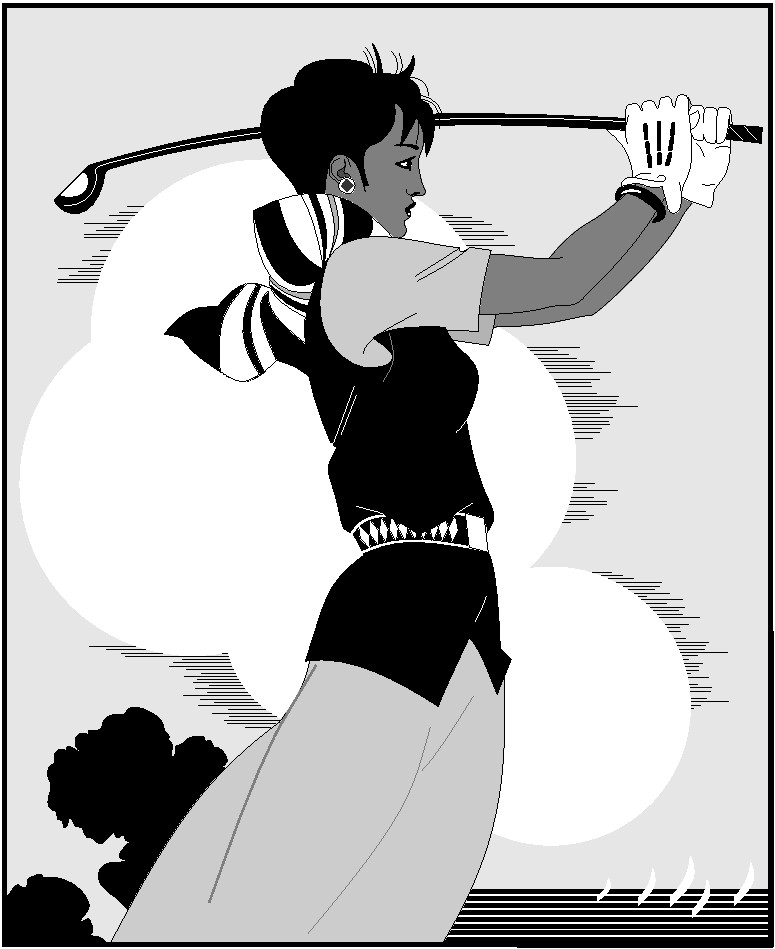
\includegraphics[width = 0.4\textwidth]{golfer}
%\bicaption[golfer5]{}{\xiaosi[0]打高尔夫球的人}{Fig.$\!$}{The person playing golf}\vspace{-1em}
\caption{\xiaosi[0]打高尔夫球的人}
\end{figure}

附录中公式的示例:
\begin{align}
a & = b \times c \\
E & = m c^2
\label{eq}
\end{align}

\chapter{这个星球上最好的免费Linux软件列表}[List of the Best Linux Software in our Planet]
\section{系统}

\href{http://fvwm.org/}{FVWM自从上世纪诞生以来,此星球最强大的窗口管理器。}
推荐基于FVWM的桌面设计hifvwm:\href{https://github.com/dustincys/hifvwm}{https://github.com/dustincys/hifvwm}。

\subsection{hifvwm的优点}

\begin{enumerate}
	\item 即使打开上百个窗口也不会“蒙圈”,对比win或mac都无法做到。计算机性能越来越强大,窗口任务的管理必须要升级到打怪兽级别。
	\item 二维可视化任务栏。
	\item 自动同步Bing搜索主页的壁纸。每次电脑开机,午夜零点自动更新,用户
		也可以手动更新,从此审美再也不疲劳。
	\item 切换窗口自动聚焦到最上面的窗口。使用键盘快捷键切换窗口时候,减少
		操作过程,自动聚焦到目标窗口。这一特性是虚拟窗口必须的人性化设
		计。
	\item 类似window右下角的功能的最小化窗口来显示桌面的功能此处类似
		win7/win10,实现在一个桌面之内操作多个任务。
	\item 任务栏结合标题栏。采用任务栏和标题栏结合,节省空间。
	\item 同类窗口切换。可以在同类窗口之内类似alt-tab的方式切换。
	\item ……
\end{enumerate}

\section{其他}

\href{https://github.com/goldendict/goldendict}{goldendict 星球最强大的桌面字典。}

\href{https://github.com/yarrick/iodine}{iodine,“HIT-WLAN + 锐捷”时代的福音。}

\href{http://www.aircrack-ng.org/}{aircrack,Wifi“安全性评估”工具,自由上网,
  就是隔壁寝室网络会变慢一点。}

\href{https://www.ledger-cli.org/}{ledger,前“金融区块链”时代最好的复式记账系统。}

\href{https://orgmode.org/}{orgmode,最强大的笔记系统,从来没有之一。}

\href{https://www.jianguoyun.com/}{坚果云,国内一款支持WebDav的云盘系统,国内真正的云盘没有之一。}

\href{https://notmuchmail.org/}{notmuch, 目前最好的邮件管理工具,还在为每天几百
  个email苦恼?几百个这些都不算多,notmuch。}

\section{vim}
实现中英文每一句一行,以及实现每一句折叠断行的简单正则式,tex源码更加乖乖。
\begin{lstlisting}
vnoremap <leader>fae J:s/[.!?]\zs\s\+/\="\r".matchstr(getline('.'), '^\s*')/g<CR>
vnoremap <leader>fac J:s/[。!?]/\=submatch(0)."\n".matchstr(getline('.'), '^\s*')/g<CR>
vnoremap <leader>fle :!fmt -80 -s<CR>
\end{lstlisting}

% \end{appendix}
% \end{latex}
%
% \subsubsection{所发表文章}
% \DescribeEnv{publication}
% 虽然在\PGR\UGR\ 中都没有明确规定此处的格式,但按照旧模板PlutoThesis,此处格式
% 非常复杂。此处仍然使用旧模板中的设置方法。
% \begin{latex}
% \begin{publication}
% \noindent\textbf{(一)发表的学术论文}
% \begin{publist}
% \item	XXX,XXX. Static Oxidation Model of Al-Mg/C Dissipation Thermal Protection Materials[J]. Rare Metal Materials and Engineering, 2010, 39(Suppl. 1): 520-524.(SCI~收录,IDS号为~669JS,IF=0.16)
% \item XXX,XXX. 精密超声振动切削单晶铜的计算机仿真研究[J]. 系统仿真学报,2007,19(4):738-741,753.(EI~收录号:20071310514841)
% \item XXX,XXX. 局部多孔质气体静压轴向轴承静态特性的数值求解[J]. 摩擦学学报,2007(1):68-72.(EI~收录号:20071510544816)
% \item XXX,XXX. 硬脆光学晶体材料超精密切削理论研究综述[J]. 机械工程学报,2003,39(8):15-22.(EI~收录号:2004088028875)
% \item XXX,XXX. 基于遗传算法的超精密切削加工表面粗糙度预测模型的参数辨识以及切削参数优化[J]. 机械工程学报,2005,41(11):158-162.(EI~收录号:2006039650087)
% \item XXX,XXX. Discrete Sliding Mode Cintrok with Fuzzy Adaptive Reaching Law on 6-PEES Parallel Robot[C]. Intelligent System Design and Applications, Jinan, 2006: 649-652.(EI~收录号:20073210746529)
% \end{publist}
%
% \noindent\textbf{(二)申请及已获得的专利(无专利时此项不必列出)}
% \begin{publist}
% \item XXX,XXX. 一种温热外敷药制备方案:中国,88105607.3[P]. 1989-07-26.
% \end{publist}
%
% \noindent\textbf{(三)参与的科研项目及获奖情况}
% \begin{publist}
% \item	XXX,XXX. XX~气体静压轴承技术研究, XX~省自然科学基金项目.课题编号:XXXX.
% \item XXX,XXX. XX~静载下预应力混凝土房屋结构设计统一理论. 黑江省科学技术二等奖, 2007.
% \end{publist}
% %\vfill
% %\hangafter=1\hangindent=2em\noindent
% %\setlength{\parindent}{2em}
% \end{publication}
% \end{latex}
%
% \subsubsection{索引}
% \DescribeEnv{ceindex}
% 我工要求中英文双语索引。后文中的自动索引实际上不需要用户干预。
%\begin{latex}
% \begin{ceindex}
%   %如果想要手动加索引,注释掉以下这一样,用wordlist环境
% \printsubindex*
% \end{ceindex}
%\end{latex}
% 手工添加索引的方法不推荐,模板中将去除该功能。
% \subsubsection{授权}
% \DescribeMacro{\authorization}
% 授权页中的签名和日期是需要手写,不需要人工干预。具体示例在\file{main.tex}中。
%\begin{latex}
% \authorization[authorization.pdf] %添加扫描页的命令,与上互斥
%\end{latex}
%
% \subsubsection{致谢声明}
% \DescribeEnv{acknowledgement}
% 把致谢做成一个环境更好一些,直接往里面写感谢的话就可以啦!
%
% \begin{latex}
% \begin{acknowledgement}
%   …
%   感谢\heu\LaTeX\ 论文模板\heuthesis\ !
% \end{acknowledgement}
% \end{latex}
%
%
% \subsubsection{简历}
% \DescribeEnv{resume}
% 个人简历。
% 实际上,致谢和个人简历是自由发挥的地区,字体,文体,格式,内容,完全自己决定。
% \begin{latex}
% \begin{resume}
% XXXX~年~XX~月~XX~日出生于~XXXX。
%
% XXXX~年~XX~月考入~XX~大学~XX~院(系)XX~专业,XXXX~年~XX~月本科毕业并获得~XX~学学士学位。
%
% XXXX~年~XX~月------XXXX~年~XX~月在~XX~大学~XX~院(系)XX~学科学习并获得~XX~学硕士学位。
%
% XXXX~年~XX~月------XXXX~年~XX~月在~XX~大学~XX~院(系)XX~学科学习并获得~XX~学博士学位。
%
% 获奖情况:如获三好学生、优秀团干部、X~奖学金等(不含科研学术获奖)。
%
% 工作经历:
% \end{resume}
% \end{latex}
%
% \subsection{其它}
% 模板的配置文件 \file{heuthesisbook.cfg} 中定义了很多固定词汇,一般无须修改。如果有特殊需求,
% 推荐在导言区使用 \cs{renewcommand}。
%
%
% \subsection{捐助}
% \changes{v1.0.1}{2017/08/27}{添加了捐助、矢量化本科论文模板的图片logo}
% 各位刀客和大侠如用的嗨,要解囊相助,请支付宝赞助
% 参照图\ref{zfb}~中提示操作(二维码被矢量化后之后去
% 除了头像等冗余无用的部分~)。
% \begin{figure}[h]
% \centering\includegraphics[width=0.5\textwidth]{zfb.eps}
% \caption{支付宝}
% \label{zfb}
% \end{figure}
%
% \StopEventually{\PrintChanges\PrintIndex}
% \clearpage
%
% \section{实现细节}
%
% \subsection{基本信息}
% \changes{v3.0.0}{2020/5/20}{更改原cls文件名为heuthesisbook}
%    \begin{macrocode}
%<*bst>
ENTRY                                             % class Entry {
{                                                 % public:
  author                                          %   String author;
  editor                                          %   String editor;
  translator                                      %   String translator;
  title                                           %   String title;
  edition                                         %   String edition;
  address                                         %   String address;
  publisher                                       %   String publisher;
  pages                                           %   String pages;
  year                                            %   String year;
  date                                            %   String date;
  modifydate                                      %   String modifydate;
  citedate                                        %   String citedate;
  url                                             %   String url;
  doi                                             %   String doi;
  language                                        %   String language;
  booktitle                                       %   String booktitle;
  journal                                         %   String journal;
  chapter                                         %   String chapter;
  series                                          %   String series;
  volume                                          %   String volume;
  number                                          %   String number;
  version 										  %	  String version;
  month                                           %   String month;
  school                                          %   String school;
  institution                                     %   String institution;
  organization                                    %   String organization;
  type                                            %   String type;
  howpublished                                    %   String howpublished;
  eid                                             %   String eid;
  key                                             %   String key;
  country                                         %   String country;
  patentid                                        %   String patentid;
  media                                           %   String media;
} {                                               %   //  declare integer variables
  required                                        %   int required;  // withther the bibfield is required
} {                                               %   //  declare String variables
  label                                           %   String label;           //  label for the entry
  mark                                            %   String mark;            //  mark for the entry
                                                  %   //  there is ahidden entry variable sort.key$
                                                  %   String sort_key;
}                                                 % }
                                                  %
%%%%%%%%%%%%%%%%%%%%%%%%%%%%%%%%%%%%%%%%%%%%%%%%%%%%%%%%%%%%%%%%%%%%%%%%%%%%%%%
                                                  %
INTEGERS {                                        % //  declare global int variables
  entry.count                                     % static int entry_count;          // number of entries
  longest.label.width                             % static int longest_label_width;  // width of the longest label
  i                                               % static int i;
  j                                               % static int j;
  k                                               % static int k;
}                                                 %
                                                  %
%%%%%%%%%%%%%%%%%%%%%%%%%%%%%%%%%%%%%%%%%%%%%%%%%%%%%%%%%%%%%%%%%%%%%%%%%%%%%%%
                                                  %
STRINGS {                                         % //  declare global String variables
  longest.label                                   % static String longest_label;     //  the longest label
  s                                               % static String s;
  t                                               % static String t;
}                                                 %
                                                  %
%%%%%%%%%%%%%%%%%%%%%%%%%%%%%%%%%%%%%%%%%%%%%%%%%%%%%%%%%%%%%%%%%%%%%%%%%%%%%%%

% define global static constants
FUNCTION {true} 				{#1}
FUNCTION {false} 				{#0}
FUNCTION {debug.enabled} 		{true}
FUNCTION {cap.volume.en} 		{"Vol~"}
FUNCTION {cap.volume.zh} 		{"卷"}
FUNCTION {cap.edition.en} 		{"~ed"}
FUNCTION {cap.edition.zh} 		{"版"}
FUNCTION {cap.anonymous.en} 	{"Anon"}
FUNCTION {cap.anonymous.zh} 	{"佚名"}
FUNCTION {cap.no.address.en} 	{"[S.l.]"}
FUNCTION {cap.no.address.zh} 	{"[出版地不详]"}
FUNCTION {cap.no.publisher.en} 	{"[s.n.]"}
FUNCTION {cap.no.publisher.zh} 	{"[出版者不详]"}
FUNCTION {cap.et.al.en} 		{", et~al"}
FUNCTION {cap.et.al.zh} 		{", 等"}
FUNCTION {cap.translate.en} 	{"~trans"}
FUNCTION {cap.translate.zh} 	{"译"}
FUNCTION {cap.doi.url} 			{"http://dx.doi.org/"}
FUNCTION {cap.st.en} 			{"st"}
FUNCTION {cap.nd.en} 			{"nd"}
FUNCTION {cap.rd.en} 			{"rd"}
FUNCTION {cap.th.en} 			{"th"}

FUNCTION {cap.space}      {" "}
FUNCTION {cap.period} 		{"\@. "}
FUNCTION {cap.comma} 			{"\@, "}
%    \end{macrocode}
% 似乎GBT2005冒号前面不需要有空格,此处删除
% \changes{v3.0.14}{2020/12/22}{似乎GBT2005冒号前面不需要有空格,此处删除}
%    \begin{macrocode}
FUNCTION {cap.colon} 			{"\textnormal{: }"}
FUNCTION {cap.double.slash} 	{" //\thinspace{}"}
FUNCTION {cap.dash} 			{"\textnormal{-}"}

% Predefined latex command used to format the style of bibitems
FUNCTION {env.bibbegin} 		{ "\begin{thebibliography}" }
FUNCTION {env.bibend}   		{ "\end{thebibliography}" }
FUNCTION {cmd.bibauthor} 		{ "\providecommand{\bibauthor}[1]{#1}" }
FUNCTION {cmd.bibeditor} 		{ "\providecommand{\bibeditor}[1]{#1}" }
FUNCTION {cmd.bibtranslator} 	{ "\providecommand{\bibtranslator}[1]{#1}" }
FUNCTION {cmd.bibtitle} 		{ "\providecommand{\bibtitle}[1]{#1}" }
FUNCTION {cmd.bibbooktitle} 	{ "\providecommand{\bibbooktitle}[1]{#1}" }
FUNCTION {cmd.bibjournal} 		{ "\providecommand{\bibjournal}[1]{#1}" }
FUNCTION {cmd.bibmark} 			{ "\providecommand{\bibmark}[1]{\mbox{#1}}" }
FUNCTION {cmd.bibcountry} 		{ "\providecommand{\bibcountry}[1]{#1}" }
FUNCTION {cmd.bibpatentid} 		{ "\providecommand{\bibpatentid}[1]{#1}" }
FUNCTION {cmd.bibedition} 		{ "\providecommand{\bibedition}[1]{#1}" }
FUNCTION {cmd.biborganization} 	{ "\providecommand{\biborganization}[1]{#1}" }
FUNCTION {cmd.bibaddress} 		{ "\providecommand{\bibaddress}[1]{#1}" }
FUNCTION {cmd.bibpublisher} 	{ "\providecommand{\bibpublisher}[1]{#1}" }
FUNCTION {cmd.bibinstitution}	{ "\providecommand{\bibinstitution}[1]{#1}" }
FUNCTION {cmd.bibschool} 		{ "\providecommand{\bibschool}[1]{#1}" }
FUNCTION {cmd.bibvolume} 		{ "\providecommand{\bibvolume}[1]{#1}" }
FUNCTION {cmd.bibnumber} 		{ "\providecommand{\bibnumber}[1]{#1}" }
FUNCTION {cmd.bibversion} 		{ "\providecommand{\bibversion}[1]{#1}" }
FUNCTION {cmd.bibpages} 		{ "\providecommand{\bibpages}[1]{#1}" }
FUNCTION {cmd.bibmodifydate}	{ "\providecommand{\bibmodifydate}[1]{#1}" }
FUNCTION {cmd.bibcitedate} 		{ "\providecommand{\bibcitedate}[1]{#1}" }
FUNCTION {cmd.bibyear} 			{ "\providecommand{\bibyear}[1]{#1}" }
FUNCTION {cmd.bibdate} 			{ "\providecommand{\bibdate}[1]{#1}" }
FUNCTION {cmd.biburl} 			{ "\providecommand{\biburl}[1]{\newline\url{#1}}" }

%%%%%%%%%%%%%%%%%%%%%%%%%%%%%%%%%%%%%%%%%%%%%%%%%%%%%%%%%%%%%%%%%%%%%%%%%%%%%%%
                                                  %
FUNCTION {log.str} {                              % void Entry::log_str(String value, String message)
  debug.enabled {                                 %   if (debug_enabled == 1) {
    "DEBUG: " swap$ * " - '" *                    %     message = "DEBUG: " + message + " - '";
    swap$ *                                       %     message = message + value;
    "'" *                                         %     message = message + "'";
    top$                                          %     log(message);
  } {                                             %   } else {
    pop$ pop$                                     %     return;
  } if$                                           %   }
}                                                 % }
                                                  %
%%%%%%%%%%%%%%%%%%%%%%%%%%%%%%%%%%%%%%%%%%%%%%%%%%%%%%%%%%%%%%%%%%%%%%%%%%%%%%%
                                                  %
FUNCTION {log.int} {                              % int Entry::log_int(int value, String message)
  debug.enabled {                                 %   if (debug_enabled == 1) {
    "DEBUG: " swap$ * " - " *                     %     message = "DEBUG: " + message + " - ";
    swap$ int.to.str$ *                           %     message = message + int_to_str(value);
    top$                                          %     log(message);
  } {                                             %   } else {
    pop$ pop$                                     %     return;
  } if$                                           %   }
}                                                 % }
                                                  %
%%%%%%%%%%%%%%%%%%%%%%%%%%%%%%%%%%%%%%%%%%%%%%%%%%%%%%%%%%%%%%%%%%%%%%%%%%%%%%%
                                                  %
FUNCTION {not} {                                  % int Entry::not(int x) {
  {                                               %   if (x == 1) {
    false                                         %     return false;
  } {                                             %   } else {
    true                                          %     return true;
  } if$                                           %   }
}                                                 % }
                                                  %
%%%%%%%%%%%%%%%%%%%%%%%%%%%%%%%%%%%%%%%%%%%%%%%%%%%%%%%%%%%%%%%%%%%%%%%%%%%%%%%
                                                  %
FUNCTION {and} {                                  % int Entry::and(int x, int y) {
  {                                               %   if (y == 1) {
    skip$                                         %     return x;
  } {                                             %   } else {
    pop$ false                                    %     return false;
  } if$                                           %   }
}                                                 % }
                                                  %
%%%%%%%%%%%%%%%%%%%%%%%%%%%%%%%%%%%%%%%%%%%%%%%%%%%%%%%%%%%%%%%%%%%%%%%%%%%%%%%
                                                  %
FUNCTION {or} {                                   % int Entry::or(int x, int y) {
  {                                               %   if (y == 1) {
    pop$ true                                     %     return true;
  } {                                             %   } else {
    skip$                                         %     return x;
  } if$                                           %   }
}                                                 % }
                                                  %
%%%%%%%%%%%%%%%%%%%%%%%%%%%%%%%%%%%%%%%%%%%%%%%%%%%%%%%%%%%%%%%%%%%%%%%%%%%%%%%
                                                  % //  calculate the length in characters of a string
                                                  % //  We need this function since text.length$ is NOT
                                                  % //  the length in characters.
INTEGERS {length.i}                               % static int length_i;
FUNCTION {length} {                               % int Entry::length(String str) {
  duplicate$ empty$ {                             %   if (empty(str)) {
    pop$ #0                                       %     return 0;
  } {                                             %   } else {
    #1 'length.i :=                               %     length_i = 1;
    false                                         %     int stop = false;
    {not} {                                       %     while (! stop) {
      duplicate$ length.i #1 substring$           %       String tmp = substring(str, length_i, 1);
      "" = {                                      %       if (tmp == "") {
        true                                      %         stop = true;
      } {                                         %       } else {
        length.i #1 + 'length.i :=                %         length_i = length_i + 1;
        false                                     %         stop = false;
      } if$                                       %       }
    } while$                                      %     }
    pop$ length.i #1 -                            %     return length_i - 1;
  } if$                                           %   }
}                                                 % }
                                                  %
%%%%%%%%%%%%%%%%%%%%%%%%%%%%%%%%%%%%%%%%%%%%%%%%%%%%%%%%%%%%%%%%%%%%%%%%%%%%%%%
                                                  %
FUNCTION {is.digit} {                             % int Entry::is_digit(String ch) {
  chr.to.int$                                     %   int ascii = chr_to_int(ch);
  duplicate$ "0" chr.to.int$ < {                  %   if (ascii < chr_to_int("0")) {
    pop$ false                                    %     return false;
  } {                                             %   } else {
    "9" chr.to.int$ > {                           %     if (ascii > chr_to_int("9")) {
      false                                       %       return false;
    } {                                           %     } else {
      true                                        %       return true;
    } if$                                         %     }
  } if$                                           %   }
}                                                 % }
                                                  %
%%%%%%%%%%%%%%%%%%%%%%%%%%%%%%%%%%%%%%%%%%%%%%%%%%%%%%%%%%%%%%%%%%%%%%%%%%%%%%%
                                                  % // test if str is a number
FUNCTION {is.number} {                            % int Entry::is_number(String str) {
  duplicate$ empty$ not swap$                     %   int result = (! empty(str));
  { duplicate$ empty$ not} {                      %   while (! empty(str)) {
    duplicate$ #1 #1 substring$ is.digit {        %     if (is_digit(substring(str, 1, 1))) {
      #2 global.max$ substring$                   %       str = substring(str, 2, global_max);
    } {                                           %     } else {
      pop$ pop$ false                             %       result = false;
      ""                                          %       str = "";
    } if$                                         %     }
  } while$                                        %   }
  pop$                                            %   return result;
}                                                 % }
                                                  %
%%%%%%%%%%%%%%%%%%%%%%%%%%%%%%%%%%%%%%%%%%%%%%%%%%%%%%%%%%%%%%%%%%%%%%%%%%%%%%%
                                                  % // extract the number prefix of str
FUNCTION {extract.number} {                       % String Entry::extract_number(String str) {
  duplicate$                                      %   String suffix = str;
  duplicate$ length swap$                         %   int n = length(str);
  duplicate$ empty$                               %   int stop = empty(suffix);
  { not } {                                       %   while (! stop) {
    duplicate$ #1 #1 substring$ is.digit {        %     if (is_digit(substring(suffix, 1, 1))) {
      #2 global.max$ substring$                   %       suffix = substring(suffix, 2, global_max);
      duplicate$ empty$                           %       stop = empty(suffix);
    } {                                           %     } else {
      true                                        %       stop = true;
    } if$                                         %     }
  } while$                                        %   }
  length -                                        %   int n = n - length(suffix);
  #1 swap$ substring$                             %   return substring(str, 1, n);
}                                                 % }
                                                  %
%%%%%%%%%%%%%%%%%%%%%%%%%%%%%%%%%%%%%%%%%%%%%%%%%%%%%%%%%%%%%%%%%%%%%%%%%%%%%%%
                                                  %
FUNCTION {get.last.chr} {                         % String Entry::get_last_chr(String str) {
  duplicate$ length                               %   int n = length(str);
  duplicate$ #0 = {                               %   if (n == 0) {
    pop$                                          %     return str;
  } {                                             %   } else {
    #1 substring$                                 %     return substring(str, n, 1);
  } if$                                           %   }
}                                                 % }
                                                  %
%%%%%%%%%%%%%%%%%%%%%%%%%%%%%%%%%%%%%%%%%%%%%%%%%%%%%%%%%%%%%%%%%%%%%%%%%%%%%%%
                                                  %
FUNCTION {get.ordinal.suffix.en} {                % String Entry::get_ordinal_suffix_en(String ch) {
  duplicate$ "1" = {                              %   if (num == "1") {
    pop$ cap.st.en                                %     return cap_st_en;
  } {                                             %   } else {
    duplicate$ "2" = {                            %     if (num == "2") {
      pop$ cap.nd.en                              %       return cap_nd_en;
    } {                                           %     } else {
      duplicate$ "3" = {                          %       if (num == "3") {
        pop$ cap.rd.en                            %         return cap_rd_en;
      } {                                         %       } else {
        pop$ cap.th.en                            %         return cap_th_en;
      } if$                                       %       }
    } if$                                         %     }
  } if$                                           %   }
}                                                 % }
                                                  %
%%%%%%%%%%%%%%%%%%%%%%%%%%%%%%%%%%%%%%%%%%%%%%%%%%%%%%%%%%%%%%%%%%%%%%%%%%%%%%%
                                                  %
FUNCTION {num.to.ordinal.en} {                    % String Entry::num_to_ordinal_en(String num) {
  duplicate$ empty$ {                             %   if (empty(num)) {
    skip$                                         %     return num;
  } {                                             %   } else {
    duplicate$ get.last.chr                       %     String ch = get_last_chr(num);
    get.ordinal.suffix.en                         %     String str = get_ordinal_suffix_en(ch);
    *                                             %     reutrn num + str;
  } if$                                           %   }
}                                                 % }
                                                  %
%%%%%%%%%%%%%%%%%%%%%%%%%%%%%%%%%%%%%%%%%%%%%%%%%%%%%%%%%%%%%%%%%%%%%%%%%%%%%%%
                                                  %
STRINGS {remove.dots.result}                      % static String remove_dots_result;
                                                  %
FUNCTION {remove.dots} {                          % String Entry::remove_dots(String str) {
  "" 'remove.dots.result :=                       %   remove_dots_result = "";
  { duplicate$ empty$ not } {                     %   while (! empty(str)) {
    duplicate$ #1 #2 substring$                   %     String tmp = substring(str, 1, 2);
    "\." = {                                      %     if (tmp == "\.") {
      #3 global.max$ substring$                   %       str = substring(str, 3, global_max);
    } {                                           %     } else {
      duplicate$ #1 #1 substring$                 %       tmp = substring(str, 1, 1);
      duplicate$ "." = {                          %       if (tmp == ".") {
        pop$ #2 global.max$ substring$            %         str = substring(str, 2, global_max);
      } {                                         %       } else {
        remove.dots.result swap$ *                %         tmp = remove_dots_result + tmp;
        'remove.dots.result :=                    %         remove_dots_result = tmp;
        #2 global.max$ substring$                 %         str = substring(str, 2, global_max);
      } if$                                       %       }
    } if$                                         %     }
  } while$                                        %   }
  pop$ remove.dots.result                         %   return remove_dots_result;
}                                                 % }
                                                  %
%%%%%%%%%%%%%%%%%%%%%%%%%%%%%%%%%%%%%%%%%%%%%%%%%%%%%%%%%%%%%%%%%%%%%%%%%%%%%%%
                                                  %
FUNCTION {add.brace} {                            % String Entry::add_brace(String str) {
  "{" swap$ * "}" *                               %   return "{" + str + "}";
}                                                 % }
                                                  %
%%%%%%%%%%%%%%%%%%%%%%%%%%%%%%%%%%%%%%%%%%%%%%%%%%%%%%%%%%%%%%%%%%%%%%%%%%%%%%%
                                                  %
FUNCTION {add.bracket} {                          % String Entry::bracket(String str) {
  "(" swap$ * ")" *                               %   return "(" + str + ")";
}                                                 % }
                                                  %
%%%%%%%%%%%%%%%%%%%%%%%%%%%%%%%%%%%%%%%%%%%%%%%%%%%%%%%%%%%%%%%%%%%%%%%%%%%%%%%
                                                  %
FUNCTION {add.squarebracket} {                    % String Entry::add_squarebracket(String str) {
  "[" swap$ * "]" *                               %   return "[" + str + "]";
}                                                 % }
                                                  %
%%%%%%%%%%%%%%%%%%%%%%%%%%%%%%%%%%%%%%%%%%%%%%%%%%%%%%%%%%%%%%%%%%%%%%%%%%%%%%%
                                                  %
FUNCTION {add.textit} {                           % String Entry::add_textit(String str) {
  "\textit{" swap$ * "}" *                        %   return "\textit{" + str + "}";
}                                                 % }
                                                  %
%%%%%%%%%%%%%%%%%%%%%%%%%%%%%%%%%%%%%%%%%%%%%%%%%%%%%%%%%%%%%%%%%%%%%%%%%%%%%%%
                                                  %
FUNCTION {add.textbf} {                           % String Entry::add_textbf(String str) {
  "\textbf{" swap$ * "}" *                        %   return "\textbf{" + str + "}";
}                                                 % }
                                                  %
%%%%%%%%%%%%%%%%%%%%%%%%%%%%%%%%%%%%%%%%%%%%%%%%%%%%%%%%%%%%%%%%%%%%%%%%%%%%%%%
                                                  % // test if str contains a dash '-'
FUNCTION {contain.dash} {                         % int Entry::contain_dash(String str) {
  false swap$                                     %   int result = false;
  { duplicate$ empty$ not} {                      %   while (! empty(str)) {
    duplicate$ #1 #1 substring$ "-" = {           %     if (substring(str, 1, 1) == "-") {
      pop$ pop$ true                              %       result = true;
      ""                                          %       str = "";
    } {                                           %     } else {
      #2 global.max$ substring$                   %       str = substring(str, 2, global_max);
    } if$                                         %     }
  } while$                                        %   }
  pop$                                            %   return result;
}                                                 % }
                                                  %
%%%%%%%%%%%%%%%%%%%%%%%%%%%%%%%%%%%%%%%%%%%%%%%%%%%%%%%%%%%%%%%%%%%%%%%%%%%%%%%
                                                  % // extract the substring before the first '-'
                                                  % // returns the string itself if no '-'
FUNCTION {extract.before.first.dash} {            % String Entry::extract_before_first_dash(String str) {
  duplicate$                                      %   String suffix = str;
  duplicate$ length swap$                         %   int n = length(str);
  duplicate$ empty$                               %   int stop = empty(suffix);
  { not } {                                       %   while (! stop) {
    duplicate$ #1 #1 substring$ "-" = {           %     if (substring(suffix, 1, 1) == "-") {
      true                                        %       stop = true;
    } {                                           %     } else {4r
      #2 global.max$ substring$                   %       suffix = substring(suffix, 2, global_max);
      duplicate$ empty$                           %       stop = empty(suffix);
    } if$                                         %     }
  } while$                                        %   }
  length -                                        %   int n = n - length(suffix);
  #1 swap$ substring$                             %   return substring(str, 1, n);
}                                                 % }
                                                  %
%%%%%%%%%%%%%%%%%%%%%%%%%%%%%%%%%%%%%%%%%%%%%%%%%%%%%%%%%%%%%%%%%%%%%%%%%%%%%%%
                                                  % // extract the substring after the first '-'
                                                  % // returns the string itself if no '-'
FUNCTION {extract.after.first.dash} {             % String Entry::extract_after_first_dash(String str) {
  duplicate$                                      %   String suffix = str;
  duplicate$ empty$                               %   int stop = empty(suffix);
  { not } {                                       %   while (! stop) {
    duplicate$ #1 #1 substring$ "-" = {           %     if (substring(suffix, 1, 1) == "-") {
      true                                        %       stop = true;
    } {                                           %     } else {4r
      #2 global.max$ substring$                   %       suffix = substring(suffix, 2, global_max);
      duplicate$ empty$                           %       stop = empty(suffix);
    } if$                                         %     }
  } while$                                        %   }
  duplicate$ empty$ {                             %   if (empty(suffix)) {
    pop$                                          %     return str;
  } {                                             %   } else {
    swap$ pop$ #2 global.max$ substring$          %     return substring(suffix, 2, global_max);
  } if$                                           %   }
}                                                 % }
                                                  %
%%%%%%%%%%%%%%%%%%%%%%%%%%%%%%%%%%%%%%%%%%%%%%%%%%%%%%%%%%%%%%%%%%%%%%%%%%%%%%%
                                                  % // extract the substring after the last '-'
                                                  % // returns the empty string if no '-'
FUNCTION {extract.after.last.dash} {              % String Entry::extract_after_last_dash(String str) {
  duplicate$ contain.dash not {                   %   if (! contain_dash(str)) {
    pop$ ""                                       %     return "";
  } {                                             %   } else {
    {duplicate$ contain.dash} {                   %     while (contain_dash(str)) {
      extract.after.first.dash                    %       str = extract_after_first_dash(str);
    } while$                                      %     }
                                                  %     return str;
  } if$                                           %   }
}                                                 % }
                                                  %
%%%%%%%%%%%%%%%%%%%%%%%%%%%%%%%%%%%%%%%%%%%%%%%%%%%%%%%%%%%%%%%%%%%%%%%%%%%%%%%
                                                  %
FUNCTION {trim.start} {                           % String Entry::trim_start(String str) {
  {duplicate$ #1 #1 substring$ " " =} {           %   while (substring(str, 1, 1) == " ") {
    #2 global.max$ substring$                     %     str = substring(str, 2, global_max);
  } while$                                        %   }
                                                  %   return str;
}                                                 % }
                                                  %
%%%%%%%%%%%%%%%%%%%%%%%%%%%%%%%%%%%%%%%%%%%%%%%%%%%%%%%%%%%%%%%%%%%%%%%%%%%%%%%
                                                  %
FUNCTION {trim.end} {                             % String Entry::trim_end(String str) {
  {duplicate$ get.last.chr " " =} {               %   while (get_last_chr(str) == " ") {
    duplicate$ length #1 -                        %     int n = length(str) - 1;
    #1 swap$ substring$                           %     str = substring(str, 1, n);
  } while$                                        %   }
                                                  %   return str;
}                                                 % }
                                                  %
%%%%%%%%%%%%%%%%%%%%%%%%%%%%%%%%%%%%%%%%%%%%%%%%%%%%%%%%%%%%%%%%%%%%%%%%%%%%%%%
                                                  %
FUNCTION {trim} {                                 % String Entry::trim(String str) {
  trim.start                                      %   str = trim_start(str);
  trim.end                                        %   return trim_end(str);
}                                                 % }
                                                  %
%%%%%%%%%%%%%%%%%%%%%%%%%%%%%%%%%%%%%%%%%%%%%%%%%%%%%%%%%%%%%%%%%%%%%%%%%%%%%%%
                                                  %
FUNCTION {start.bibitem} {                        % void Entry::start_bibitem() {
  newline$                                        %   writeln();
  "\bibitem{" cite$ * "}" * write$                %   write("\bibitem{" + this.cite + "}");
  newline$                                        %   writeln();
}                                                 % }
                                                  %
%%%%%%%%%%%%%%%%%%%%%%%%%%%%%%%%%%%%%%%%%%%%%%%%%%%%%%%%%%%%%%%%%%%%%%%%%%%%%%%
                                                  %
FUNCTION {end.bibitem} {                          % void Entry::end_bibitem() {
  cap.period write$                               %   write(cap_period);
  newline$                                        %   writeln();
}                                                 % }
                                                  %
%%%%%%%%%%%%%%%%%%%%%%%%%%%%%%%%%%%%%%%%%%%%%%%%%%%%%%%%%%%%%%%%%%%%%%%%%%%%%%%
                                                  %
FUNCTION {is.in.chinese} {                        % int Entry::is_in_chinese() {
  language empty$ {                               %   if (empty(this.language)) {
    false                                         %     return false;
  } {                                             %   } else {
    language "zh" = {                             %     if (this.language == "zh") {
      true                                        %       return true;
    } {                                           %     } else {
      false                                       %       return false;
    } if$                                         %     }
  } if$                                           %   }
}                                                 % }
                                                  %
%%%%%%%%%%%%%%%%%%%%%%%%%%%%%%%%%%%%%%%%%%%%%%%%%%%%%%%%%%%%%%%%%%%%%%%%%%%%%%%
                                                  %
FUNCTION {is.online} {                            % int Entry::is_online() {
  url empty$ not {                                %   if (! empty(this.url)) {
    true                                          %     return true;
  } {                                             %   } else {
    doi empty$ not {                              %     if (! empty(this.doi)) {
      true                                        %       return true;
    } {                                           %     } else {
      false                                       %       return false;
    } if$                                         %     }
  } if$                                           %   }
}                                                 % }
                                                  %
%%%%%%%%%%%%%%%%%%%%%%%%%%%%%%%%%%%%%%%%%%%%%%%%%%%%%%%%%%%%%%%%%%%%%%%%%%%%%%%
                                                  %
FUNCTION {set.mark} {                             % void Entry::set_mark(String mark) {
  'mark :=                                        %   this.mark = mark;
  is.online {                                     %   if (is_online()) {
    mark "/OL" * 'mark :=                         %     this.mark = this.mark + "/OL";
  } {                                             %   } else {
    media empty$ not {                            %     if (! empty(this.media)) {
      mark "/" * media * 'mark :=                 %       this.mark = this.mark + "/" + this.media;
    } 'skip$ if$                                  %     }
  } if$                                           %   }
}                                                 % }
                                                  %
%%%%%%%%%%%%%%%%%%%%%%%%%%%%%%%%%%%%%%%%%%%%%%%%%%%%%%%%%%%%%%%%%%%%%%%%%%%%%%%
                                                  %
FUNCTION {cap.volume} {                           % String Entry::cap_volume() {
  is.in.chinese {                                 %   if (is_in_chinese()) {
    cap.volume.zh                                 %     return cap_volume_zh;
  } {                                             %   } else {
    cap.volume.en                                 %     return cap_volume_en;
  } if$                                           %   }
}                                                 % }
                                                  %
%%%%%%%%%%%%%%%%%%%%%%%%%%%%%%%%%%%%%%%%%%%%%%%%%%%%%%%%%%%%%%%%%%%%%%%%%%%%%%%
                                                  %
FUNCTION {cap.edition} {                          % String Entry::cap_edition() {
  is.in.chinese {                                 %   if (is_in_chinese()) {
    cap.edition.zh                                %     return cap_edition_zh;
  } {                                             %   } else {
    cap.edition.en                                %     return cap_edition_en;
  } if$                                           %   }
}                                                 % }
                                                  %
%%%%%%%%%%%%%%%%%%%%%%%%%%%%%%%%%%%%%%%%%%%%%%%%%%%%%%%%%%%%%%%%%%%%%%%%%%%%%%%
                                                  %
FUNCTION {cap.anonymous} {                        % String Entry::cap_anonymous() {
  is.in.chinese {                                 %   if (is_in_chinese()) {
    cap.anonymous.zh                              %     return cap_anonymous_zh;
  } {                                             %   } else {
    cap.anonymous.en                              %     return cap_anonymous_en;
  } if$                                           %   }
}                                                 % }
                                                  %
%%%%%%%%%%%%%%%%%%%%%%%%%%%%%%%%%%%%%%%%%%%%%%%%%%%%%%%%%%%%%%%%%%%%%%%%%%%%%%%
                                                  %
FUNCTION {cap.no.address} {                       % String Entry::cap_no_address() {
  is.in.chinese {                                 %   if (is_in_chinese()) {
    cap.no.address.zh                             %     return cap_no_address_zh;
  } {                                             %   } else {
    cap.no.address.en                             %     return cap_no_address_en;
  } if$                                           %   }
}                                                 % }
                                                  %
%%%%%%%%%%%%%%%%%%%%%%%%%%%%%%%%%%%%%%%%%%%%%%%%%%%%%%%%%%%%%%%%%%%%%%%%%%%%%%%
                                                  %
FUNCTION {cap.no.publisher} {                     % String Entry::cap_no_publisher() {
  is.in.chinese {                                 %   if (is_in_chinese()) {
    cap.no.publisher.zh                           %     return cap_no_publisher_zh;
  } {                                             %   } else {
    cap.no.publisher.en                           %     return cap_no_publisher_en;
  } if$                                           %   }
}                                                 % }
                                                  %
%%%%%%%%%%%%%%%%%%%%%%%%%%%%%%%%%%%%%%%%%%%%%%%%%%%%%%%%%%%%%%%%%%%%%%%%%%%%%%%
                                                  %
FUNCTION {cap.et.al} {                            % String Entry::cap_et_al() {
  is.in.chinese {                                 %   if (is_in_chinese()) {
    cap.et.al.zh                                  %     return cap_et_al_zh;
  } {                                             %   } else {
    cap.et.al.en                                  %     return cap_et_al_en;
  } if$                                           %   }
}                                                 % }
                                                  %
%%%%%%%%%%%%%%%%%%%%%%%%%%%%%%%%%%%%%%%%%%%%%%%%%%%%%%%%%%%%%%%%%%%%%%%%%%%%%%%
                                                  %
FUNCTION {cap.translate} {                        % String Entry::cap_translate() {
  is.in.chinese {                                 %   if (is_in_chinese()) {
    cap.translate.zh                              %     return cap_translate_zh;
  } {                                             %   } else {
    cap.translate.en                              %     return cap_translate_en;
  } if$                                           %   }
}                                                 % }
                                                  %
%%%%%%%%%%%%%%%%%%%%%%%%%%%%%%%%%%%%%%%%%%%%%%%%%%%%%%%%%%%%%%%%%%%%%%%%%%%%%%%
                                                  %
FUNCTION {format.bibinfo} {                       % String Entry::format_bibinfo(String info, String type) {
  swap$ add.brace swap$                           %   info = add_brace(info);
  "\bib" swap$ * swap$ *                          %   return "\bib" + type + info;
}                                                 % }
                                                  %
%%%%%%%%%%%%%%%%%%%%%%%%%%%%%%%%%%%%%%%%%%%%%%%%%%%%%%%%%%%%%%%%%%%%%%%%%%%%%%%
INTEGERS { nameindex namecount }                  % static int nameindex, namecount;
STRINGS  { namelist nameformat }                  % static String namelist, nameformat;
STRINGS  { firstname lastname jrname vonname}     % static String firstname, lastname, jrname, vonname;
                                                  %
FUNCTION {format.names} {                         % String Entry::format_names(String names) {
  'namelist :=                                    %   namelist = names;
  namelist num.names$ 'namecount :=               %   namecount = num_names(namelist);
  ""                                              %   String result = "";
  #0 'nameindex :=                                %   nameindex = 0;
  {nameindex namecount < nameindex #3 < and} {    %   while ((nameindex < namecount) && (nameindex < 3)) {
    nameindex #1 + 'nameindex :=                  %     nameindex = nameindex + 1;
    nameindex #1 > {                              %     if (nameindex > 1) {
      cap.comma *                                 %       result = result + cap_comma;
    } 'skip$ if$                                  %     }
    namelist nameindex "{vv}" format.name$        %     String tmp = format_name(namelist, nameindex, "{vv}");
   'vonname :=                                    %     vonname = tmp;
    namelist nameindex "{jj}" format.name$        %     tmp = format_name(namelist, nameindex, "{jj}");
    remove.dots 'jrname :=                        %     jrname = remove_dots(tmp);
    namelist nameindex "{f}" format.name$         %     tmp = format_name(namelist, nameindex, "{f}");
    remove.dots                                   %     tmp = remove_dots(tmp);
    'firstname :=                                 %     firstname = change_case(tmp, "u");
    namelist nameindex "{ll}" format.name$        %     tmp = format_name(namelist, nameindex, "{ll}");
    'lastname :=                                  %     lastname = change_case(tmp, "u");
    jrname empty$ not {                           %     if (! empty(jrname)) {
      jrname * " " *                              %       result = result + jrname + " "
    } 'skip$ if$                                  %     }
    vonname empty$ not {                          %     if (! empty(vonname)) {
      vonname * " " *                             %       result = result + vonname + " "
    } 'skip$ if$                                  %     }
    lastname empty$ not {                         %     if (! empty(lastname)) {
      lastname * " " *                            %       result = result + lastname + " "
    } 'skip$ if$                                  %     }
    firstname empty$ not {                        %     if (! empty(firstname)) {
      firstname * " " *                           %       result = result + firstname + " "
    } 'skip$ if$                                  %     }
    trim.end                                      %     result = trim_end(result);
  } while$                                        %   }
  nameindex namecount < {                         %   if (nameindex < namecount) {
    cap.et.al *                                   %     result = result + cap_et_al();
  } 'skip$ if$                                    %   }
}                                                 % }
                                                  %
                                                  %
%%%%%%%%%%%%%%%%%%%%%%%%%%%%%%%%%%%%%%%%%%%%%%%%%%%%%%%%%%%%%%%%%%%%%%%%%%%%%%%
                                                  % // format English names
FUNCTION {format.names.en} {                      % String Entry::format_names_en(String names) {
  format.names                                    %   format_names(names);
}                                                 % }
                                                  %
%%%%%%%%%%%%%%%%%%%%%%%%%%%%%%%%%%%%%%%%%%%%%%%%%%%%%%%%%%%%%%%%%%%%%%%%%%%%%%%
                                                  % // format Chinese names
FUNCTION {format.names.zh} {                      % String Entry::format_names_zh(String names) {
  format.names                                    %   format_names(names);
}                                                 % }
                                                  %
%%%%%%%%%%%%%%%%%%%%%%%%%%%%%%%%%%%%%%%%%%%%%%%%%%%%%%%%%%%%%%%%%%%%%%%%%%%%%%%
                                                  %
FUNCTION {format.author} {                        % String Emtry::format_author(String authors) {
  is.in.chinese {                                 %   if (is_in_chinese) {
    format.names.zh                               %     authors = format_names_zh(authors);
  } {                                             %   } else {
    format.names.en                               %     authors = format_names_en(authors);
  } if$                                           %   }
  "author" format.bibinfo                         %   return format_bibinfo(authors, "author");
}                                                 % }
                                                  %
%%%%%%%%%%%%%%%%%%%%%%%%%%%%%%%%%%%%%%%%%%%%%%%%%%%%%%%%%%%%%%%%%%%%%%%%%%%%%%%
                                                  %
FUNCTION {format.editor} {                        % String Emtry::format_author(String editors) {
  is.in.chinese {                                 %   if (is_in_chinese) {
    format.names.zh                               %     editors = format_names_zh(editors);
  } {                                             %   } else {
    format.names.en                               %     editors = format_names_en(editors);
  } if$                                           %   }
  "editor" format.bibinfo                         %   return format_bibinfo(editors, "editor");
}                                                 % }
                                                  %
%%%%%%%%%%%%%%%%%%%%%%%%%%%%%%%%%%%%%%%%%%%%%%%%%%%%%%%%%%%%%%%%%%%%%%%%%%%%%%%
                                                  %
FUNCTION {format.translator} {                    % String Emtry::format_translator(String translators) {
  is.in.chinese {                                 %   if (is_in_chinese) {
    duplicate$                                    %     String names = translators;
    format.names.zh                               %     translators = format_names_zh(translators);
    swap$ num.names$ #3 > {                       %     if (num_names(names) > 3) {
      cap.translate.zh *                          %       translators = translators + cap_translate_zh;
    } {                                           %     } else {
      cap.comma * cap.translate.zh *              %       translators = translators + cap_comma + cap_translate_zh;
    } if$                                         %     }
  } {                                             %   } else {
    duplicate$                                    %     String names = translators;
    format.names.en                               %     translators = format_names_en(translators);
    swap$ num.names$ #3 > {                       %     if (num_names(names) > 3) {
      cap.translate.en *                          %       translators = translators + cap_translate_en;
    } {                                           %     } else {
      cap.comma * cap.translate.en *              %       translators = translators + cap_comma + cap_translate_en;
    } if$                                         %     }
  } if$                                           %   }
  "translator" format.bibinfo                     %   return format_bibinfo(translator, "translator");
}                                                 % }
                                                  %
%%%%%%%%%%%%%%%%%%%%%%%%%%%%%%%%%%%%%%%%%%%%%%%%%%%%%%%%%%%%%%%%%%%%%%%%%%%%%%%
                                                  %
FUNCTION {format.title} {                         % String Emtry::format_title(String title) {
  "title" format.bibinfo                          %   return format_bibinfo(title, "title");
}                                                 % }
                                                  %
%%%%%%%%%%%%%%%%%%%%%%%%%%%%%%%%%%%%%%%%%%%%%%%%%%%%%%%%%%%%%%%%%%%%%%%%%%%%%%%
                                                  %
FUNCTION {format.booktitle} {                     % String Emtry::format_booktitle(String booktitle) {
  "booktitle" format.bibinfo                      %   return format_bibinfo(booktitle, "booktitle");
}                                                 % }
                                                  %
%%%%%%%%%%%%%%%%%%%%%%%%%%%%%%%%%%%%%%%%%%%%%%%%%%%%%%%%%%%%%%%%%%%%%%%%%%%%%%%
                                                  %
FUNCTION {format.mark} {                          % String Emtry::format_mark(String mark) {
  "[" swap$ * "]" *                               %   mark = "[" + mark + "]";
  "mark" format.bibinfo                           %   return format_bibinfo(mark, "mark");
}                                                 % }
                                                  %
%%%%%%%%%%%%%%%%%%%%%%%%%%%%%%%%%%%%%%%%%%%%%%%%%%%%%%%%%%%%%%%%%%%%%%%%%%%%%%%
                                                  %
FUNCTION {format.country} {                       % String Emtry::format_country(String country) {
  "country" format.bibinfo                        %   return format_bibinfo(country, "country");
}                                                 % }
                                                  %
%%%%%%%%%%%%%%%%%%%%%%%%%%%%%%%%%%%%%%%%%%%%%%%%%%%%%%%%%%%%%%%%%%%%%%%%%%%%%%%
                                                  %
FUNCTION {format.patentid} {                      % String Emtry::format_patentid(String patentid) {
  "patentid" format.bibinfo                       %   return format_bibinfo(patentid, "patentid");
}                                                 % }
                                                  %
%%%%%%%%%%%%%%%%%%%%%%%%%%%%%%%%%%%%%%%%%%%%%%%%%%%%%%%%%%%%%%%%%%%%%%%%%%%%%%%
                                                  %
FUNCTION {format.edition} {                       % String Emtry::format_edition(String edition) {
  duplicate$ is.number {                          %   if (is_number(edition)) {
    is.in.chinese {                               %     if (is_in_chinese()) {
      cap.edition.zh *                            %       edition = edition + cap_edition_zh;
    } {                                           %     } else {
      num.to.ordinal.en cap.edition.en *          %       edition = num_to_ordinal_en(edition) + cap_edition_en;
    } if$                                         %     }
  } 'skip$ if$                                    %   }
                                                  %   //  use a \mbox{} to prevent line break within edition
  "\mbox{" swap$ * "}" *                          %   edition = "\mbox{" + edition + "}";
  "edition" format.bibinfo                        %   return format_bibinfo(edition, "edition");
}                                                 % }
                                                  %
%%%%%%%%%%%%%%%%%%%%%%%%%%%%%%%%%%%%%%%%%%%%%%%%%%%%%%%%%%%%%%%%%%%%%%%%%%%%%%%
                                                  %
FUNCTION {format.organization} {                  % String Emtry::format_organization(String organization) {
  "organization" format.bibinfo                   %   return format_bibinfo(organization, "organization");
}                                                 % }
                                                  %
%%%%%%%%%%%%%%%%%%%%%%%%%%%%%%%%%%%%%%%%%%%%%%%%%%%%%%%%%%%%%%%%%%%%%%%%%%%%%%%
                                                  %
FUNCTION {format.address} {                       % String Emtry::format_address(String address) {
  "address" format.bibinfo                        %   return format_bibinfo(address, "address");
}                                                 % }
                                                  %
%%%%%%%%%%%%%%%%%%%%%%%%%%%%%%%%%%%%%%%%%%%%%%%%%%%%%%%%%%%%%%%%%%%%%%%%%%%%%%%
                                                  %
FUNCTION {format.publisher} {                     % String Emtry::format_publisher(String publisher) {
  "publisher" format.bibinfo                      %   return format_bibinfo(publisher, "publisher");
}                                                 % }
                                                  %
%%%%%%%%%%%%%%%%%%%%%%%%%%%%%%%%%%%%%%%%%%%%%%%%%%%%%%%%%%%%%%%%%%%%%%%%%%%%%%%
                                                  %
FUNCTION {format.institution} {                   % String Emtry::format_institution(String institution) {
  "institution" format.bibinfo                    %   return format_bibinfo(institution, "institution");
}                                                 % }
                                                  %
%%%%%%%%%%%%%%%%%%%%%%%%%%%%%%%%%%%%%%%%%%%%%%%%%%%%%%%%%%%%%%%%%%%%%%%%%%%%%%%
                                                  %
FUNCTION {format.school} {                        % String Emtry::format_school(String school) {
  "school" format.bibinfo                         %   return format_bibinfo(school, "school");
}                                                 % }
                                                  %
%%%%%%%%%%%%%%%%%%%%%%%%%%%%%%%%%%%%%%%%%%%%%%%%%%%%%%%%%%%%%%%%%%%%%%%%%%%%%%%
                                                  %
FUNCTION {format.year} {                          % String Emtry::format_year(String year) {
  "year" format.bibinfo                           %   return format_bibinfo(year, "year");
}                                                 % }
                                                  %
%%%%%%%%%%%%%%%%%%%%%%%%%%%%%%%%%%%%%%%%%%%%%%%%%%%%%%%%%%%%%%%%%%%%%%%%%%%%%%%
                                                  %
FUNCTION {format.date} {                          % String Emtry::format_date(String date) {
  "date" format.bibinfo                           %   return format_bibinfo(date, "date");
}                                                 % }
                                                  %
%%%%%%%%%%%%%%%%%%%%%%%%%%%%%%%%%%%%%%%%%%%%%%%%%%%%%%%%%%%%%%%%%%%%%%%%%%%%%%%
                                                  %
FUNCTION {format.journal} {                       % String Emtry::format_journal(String journal) {
  "journal" format.bibinfo                        %   return format_bibinfo(journal, "journal");
}                                                 % }
                                                  %
%%%%%%%%%%%%%%%%%%%%%%%%%%%%%%%%%%%%%%%%%%%%%%%%%%%%%%%%%%%%%%%%%%%%%%%%%%%%%%%
                                                  %
FUNCTION {format.volume} {                        % String Emtry::format_volume(String volume) {
  "volume" format.bibinfo                         %   return format_bibinfo(volume, "volume");
}                                                 % }
                                                  %
%%%%%%%%%%%%%%%%%%%%%%%%%%%%%%%%%%%%%%%%%%%%%%%%%%%%%%%%%%%%%%%%%%%%%%%%%%%%%%%
                                                  %
FUNCTION {format.number} {                        % String Emtry::format_number(String number) {
  add.bracket                                     %   number = add_bracket(number);
  "number" format.bibinfo                         %   return format_bibinfo(number, "number");
}                                                 % }
                                                  %
%%%%%%%%%%%%%%%%%%%%%%%%%%%%%%%%%%%%%%%%%%%%%%%%%%%%%%%%%%%%%%%%%%%%%%%%%%%%%%%
                                                  %
FUNCTION {format.report.number} {                 % String Emtry::format_report_number(String number) {
  "number" format.bibinfo                         %   return format_bibinfo(number, "number");
}                                                 % }
                                                  %
%%%%%%%%%%%%%%%%%%%%%%%%%%%%%%%%%%%%%%%%%%%%%%%%%%%%%%%%%%%%%%%%%%%%%%%%%%%%%%%
                                                  %
FUNCTION {format.version} {                       % String Emtry::format_version(String version) {
  "version" format.bibinfo                        %   return format_bibinfo(version, "version");
}                                                 % }
                                                  %
%%%%%%%%%%%%%%%%%%%%%%%%%%%%%%%%%%%%%%%%%%%%%%%%%%%%%%%%%%%%%%%%%%%%%%%%%%%%%%%
                                                  %
FUNCTION {format.pages} {                         % String Emtry::format_pages(String pages) {
  "pages" format.bibinfo                          %   return format_bibinfo(pages, "pages");
}                                                 % }
                                                  %
%%%%%%%%%%%%%%%%%%%%%%%%%%%%%%%%%%%%%%%%%%%%%%%%%%%%%%%%%%%%%%%%%%%%%%%%%%%%%%%
                                                  %
FUNCTION {format.modifydate} {                    % String Emtry::format_modifydate(String modifydate) {
  add.bracket                                     %   modifydate = add_bracket(modifydate);
  "modifydate" format.bibinfo                     %   return format_bibinfo(modifydate, "modifydate");
}                                                 % }
                                                  %
%%%%%%%%%%%%%%%%%%%%%%%%%%%%%%%%%%%%%%%%%%%%%%%%%%%%%%%%%%%%%%%%%%%%%%%%%%%%%%%
                                                  %
FUNCTION {format.citedate} {                      % String Emtry::format_citedate(String citedate) {
  add.squarebracket                               %   citedate = add_squarebracket(citedate);
  "citedate" format.bibinfo                       %   return format_bibinfo(citedate, "citedate");
}                                                 % }
                                                  %
%%%%%%%%%%%%%%%%%%%%%%%%%%%%%%%%%%%%%%%%%%%%%%%%%%%%%%%%%%%%%%%%%%%%%%%%%%%%%%%
                                                  %
                                                  % // NOTE: do not use the format_bibinfo() for URL,
                                                  % // since if the URL contains special symbols such
                                                  % // as '%', the \biburl{} will be broken.
FUNCTION {format.url} {                           % String Emtry::format_url(String url) {
  "\url{" swap$ * "}" *                           %   return "\url{" + url + "}";
}                                                 % }
                                                  %
%%%%%%%%%%%%%%%%%%%%%%%%%%%%%%%%%%%%%%%%%%%%%%%%%%%%%%%%%%%%%%%%%%%%%%%%%%%%%%%
                                                  %
FUNCTION {get.full.title} {                       % String Entry::get_full_title() {
  series empty$ {                                 %     if (empty(this.series)) {
    volume empty$ {                               %       if (empty(this.volume)) {
      title                                       %         return this.title;
    } {                                           %       } else {
      title cap.colon * cap.volume * volume *     %         return this.title + cap_colon + cap_volume() + this.volume;
    } if$                                         %       }
  } {                                             %     } else {
    volume empty$ {                               %       if (empty(this.volume)) {
      series cap.colon * title *                  %         return this.series + cap_colon + this.title;
    } {                                           %       } else {
      series cap.comma * cap.volume * volume *    %         String str = this.series + cap_comma + cal_volume() + this.volume;
      cap.colon * title *                         %         return str + cap_colon + this.title;
    } if$                                         %       }
  } if$                                           %     }
}                                                 % }
                                                  %
%%%%%%%%%%%%%%%%%%%%%%%%%%%%%%%%%%%%%%%%%%%%%%%%%%%%%%%%%%%%%%%%%%%%%%%%%%%%%%%
                                                  %
FUNCTION {get.full.booktitle} {                   % String Entry::get_full_booktitle() {
  series empty$ {                                 %     if (empty(this.series)) {
    volume empty$ {                               %       if (empty(this.volume)) {
      booktitle                                   %         return this.booktitle;
    } {                                           %       } else {
      booktitle cap.colon * cap.volume * volume * %         return this.booktitle + cap_colon + cap_volume() + this.volume;
    } if$                                         %       }
  } {                                             %     } else {
    volume empty$ {                               %       if (empty(this.volume)) {
      series cap.colon * booktitle *              %         return this.series + cap_colon + this.booktitle;
    } {                                           %       } else {
      series cap.comma * cap.volume * volume *    %         String str = this.series + cap_comma + cal_volume() + this.volume;
      cap.colon * booktitle *                     %         return str + cap_colon + this.booktitle;
    } if$                                         %       }
  } if$                                           %     }
}                                                 % }
                                                  %
%%%%%%%%%%%%%%%%%%%%%%%%%%%%%%%%%%%%%%%%%%%%%%%%%%%%%%%%%%%%%%%%%%%%%%%%%%%%%%%
                                                  %
FUNCTION {get.pages} {                            % String Entry::get_pages() {
  pages contain.dash {                            %   if (contain_dash(this.pages)) {
    pages extract.before.first.dash               %     String p1 = extract_before_first_dash(this.pages);
    pages extract.after.last.dash                 %     String p2 = extract_after_last_dash(this.pages);
    cap.dash swap$ * *                            %     return p1 + cap_dash + p2;
  } {                                             %   } else {
    pages                                         %     return this.pages;
  } if$                                           %   }
}                                                 % }
                                                  %
%%%%%%%%%%%%%%%%%%%%%%%%%%%%%%%%%%%%%%%%%%%%%%%%%%%%%%%%%%%%%%%%%%%%%%%%%%%%%%%
                                                  %
FUNCTION {output.author.or.editor} {              % void Entry::output_author_or_editor(int required) {
  'required :=                                    %   this.required = required;
  author empty$ not {                             %   if (! empty(this.author)) {
    author format.author write$                   %     write(format_author(this.author));
    cap.period write$                             %     write(cap_period);
  } {                                             %   } else {
    editor empty$ not {                           %     if (! empty(this.editor)) {
      editor format.editor write$                 %       write(format_editor(this.editor));
      cap.period write$                           %       write(cap_period);
    } {                                           %     } else {
      required {                                  %       if (required == 1) {
        "Require author/editor: " cite$ * warning$%         warning("Require author/editor: " + this.cite);
        cap.anonymous format.author write$        %         write(format_author(cap_anonymous()));
        cap.period write$                         %         write(cap_period);
      } 'skip$ if$                                %       }
    } if$                                         %     }
  } if$                                           %   }
}                                                 % }
                                                  %
%%%%%%%%%%%%%%%%%%%%%%%%%%%%%%%%%%%%%%%%%%%%%%%%%%%%%%%%%%%%%%%%%%%%%%%%%%%%%%%
                                                  %
FUNCTION {output.author} {                        % void Entry::output_author(int required) {
  'required :=                                    %   this.required = required;
  author empty$ not {                             %   if (! empty(this.author)) {
    author format.author write$                   %     write(format_author(this.author));
    cap.period write$                             %     write(cap_period);
  } {                                             %   } else {
    required {                                    %     if (required == 1) {
      "Require author: " cite$ * warning$         %       warning("Require author: " + this.cite);
      cap.anonymous format.author write$          %       write(format_author(cap_anonymous()));
      cap.period write$                           %       write(cap_period);
    } 'skip$ if$                                  %     }
  } if$                                           %   }
}                                                 % }
                                                  %
%%%%%%%%%%%%%%%%%%%%%%%%%%%%%%%%%%%%%%%%%%%%%%%%%%%%%%%%%%%%%%%%%%%%%%%%%%%%%%%
                                                  %
FUNCTION {output.editor} {                        % void Entry::output_editor(int required) {
  'required :=                                    %   this.required = required;
  editor empty$ not {                             %   if (! empty(this.editor)) {
    editor format.editor write$                   %     write(format_editor(this.editor));
    cap.period write$                             %     write(cap_period);
  } {                                             %   } else {
    required {                                    %     if (required == 1) {
      "Require editor: " cite$ * warning$         %       warning("Require editor: " + this.cite);
      cap.anonymous format.editor write$          %       write(format_editor(cap_anonymous()));
      cap.period write$                           %       write(cap_period);
    } 'skip$ if$                                  %     }
  } if$                                           %   }
}                                                 % }
                                                  %
%%%%%%%%%%%%%%%%%%%%%%%%%%%%%%%%%%%%%%%%%%%%%%%%%%%%%%%%%%%%%%%%%%%%%%%%%%%%%%%
                                                  %
FUNCTION {output.title} {                         % void Entry::output_title(int required) {
  'required :=                                    %   this.required = required;
  title empty$ not {                              %   if (! empty(this.title)) {
    title format.title write$                     %     write(format_title(this.title));
  } {                                             %   } else {
    required {                                    %     if (required == 1) {
      "Require title: " cite$ * warning$          %       warning("Require title: " + this.cite);
    } 'skip$ if$                                  %     }
  } if$                                           %   }
}                                                 % }
                                                  %
%%%%%%%%%%%%%%%%%%%%%%%%%%%%%%%%%%%%%%%%%%%%%%%%%%%%%%%%%%%%%%%%%%%%%%%%%%%%%%%
                                                  %
FUNCTION {output.series.volume.title} {           % void Entry::output_series_volume_title(int required) {
  'required :=                                    %   this.required = required;
  title empty$ not {                              %   if (! empty(this.title)) {
    get.full.title format.booktitle write$        %     write(format_booktitle(get_full_title()));
  } {                                             %   } else {
    required {                                    %     if (required == 1) {
      "Require title: " cite$ * warning$          %       warning("Require title: " + this.cite);
    } 'skip$ if$                                  %     }
  } if$                                           %   }
}                                                 % }
                                                  %
%%%%%%%%%%%%%%%%%%%%%%%%%%%%%%%%%%%%%%%%%%%%%%%%%%%%%%%%%%%%%%%%%%%%%%%%%%%%%%%
                                                  %
FUNCTION {output.series.volume.booktitle} {       % void Entry::output_series_volume_booktitle(int required) {
  'required :=                                    %   this.required = required;
  booktitle empty$ not {                          %   if (! empty(this.booktitle)) {
    get.full.booktitle format.booktitle write$    %     write(format_booktitle(get_full_booktitle());
  } {                                             %   } else {
    required {                                    %     if (required == 1) {
      "Require booktitle: " cite$ * warning$      %       warning("Require booktitle: " + this.cite);
    } 'skip$ if$                                  %     }
  } if$                                           %   }
}                                                 % }
                                                  %
%%%%%%%%%%%%%%%%%%%%%%%%%%%%%%%%%%%%%%%%%%%%%%%%%%%%%%%%%%%%%%%%%%%%%%%%%%%%%%%
                                                  %
FUNCTION {output.journal} {                       % void Entry::output_journal(int required) {
  'required :=                                    %   this.required = required;
  journal empty$ not {                            %   if (! empty(this.journal)) {
    cap.period write$                             %     write(cap_period);
    journal format.journal write$                 %     write(format_journal(this.journal));
  } {                                             %   } else {
    required {                                    %     if (required == 1) {
      "Require journal: " cite$ * warning$        %       warning("Require journal: " + this.cite);
    } 'skip$ if$                                  %     }
  } if$                                           %   }
}                                                 % }
                                                  %
%%%%%%%%%%%%%%%%%%%%%%%%%%%%%%%%%%%%%%%%%%%%%%%%%%%%%%%%%%%%%%%%%%%%%%%%%%%%%%%
                                                  %
FUNCTION {output.mark} {                          % void Entry::output_mark(int required) {
  'required :=                                    %   this.required = required;
  mark empty$ not {                               %   if (! empty(this.mark)) {
    mark format.mark write$                       %     write(format_mark(this.mark));
  } {                                             %   } else {
    required {                                    %     if (required == 1) {
      "Require mark: " cite$ * warning$           %       warning("Require mark: " + this.cite);
    } 'skip$ if$                                  %     }
  } if$                                           %   }
}                                                 % }
                                                  %
%%%%%%%%%%%%%%%%%%%%%%%%%%%%%%%%%%%%%%%%%%%%%%%%%%%%%%%%%%%%%%%%%%%%%%%%%%%%%%%
                                                  %
FUNCTION {output.translator} {                    % void Entry::output_translator(int required) {
  'required :=                                    %   this.required = required;
  translator empty$ not {                         %   if (! empty(this.translator)) {
    cap.period write$                             %     write(cap_period);
    translator format.translator write$           %     write(format_translator(this.translator));
  } {                                             %   } else {
    required {                                    %     if (required == 1) {
      "Require translator: " cite$ * warning$     %       warning("Require translator: " + this.cite);
    } 'skip$ if$                                  %     }
  } if$                                           %   }
}                                                 % }
                                                  %
%%%%%%%%%%%%%%%%%%%%%%%%%%%%%%%%%%%%%%%%%%%%%%%%%%%%%%%%%%%%%%%%%%%%%%%%%%%%%%%
                                                  %
FUNCTION {output.edition} {                       % void Entry::output_edition(int required) {
  'required :=                                    %   this.required = required;
  edition empty$ not {                            %   if (! empty(this.edition)) {
    cap.period write$                             %     write(cap_period);
    edition format.edition write$                 %     write(format_edition(this.edition));
  } {                                             %   } else {
    required {                                    %     if (required == 1) {
      "Require edition: " cite$ * warning$        %       warning("Require edition: " + this.cite);
    } 'skip$ if$                                  %     }
  } if$                                           %   }
}                                                 % }
                                                  %
%%%%%%%%%%%%%%%%%%%%%%%%%%%%%%%%%%%%%%%%%%%%%%%%%%%%%%%%%%%%%%%%%%%%%%%%%%%%%%%
                                                  %
FUNCTION {output.address} {                       % void Entry::output_address(int required) {
  'required :=                                    %   this.required = required;
  address empty$ not {                            %   if (! empty(this.address)) {
    cap.period write$                             %     write(cap_period);
    address format.address write$                 %     write(format_address(this.address));
  } {                                             %   } else {
    required {                                    %     if (required == 1) {
      "Require address: " cite$ * warning$        %       warning("Require address: " + this.cite);
      cap.period write$                           %       write(cap_period);
      cap.no.address format.address write$        %       write(format_address(cap_no_address()));
    } 'skip$ if$                                  %     }
  } if$                                           %   }
}                                                 % }
                                                  %
%%%%%%%%%%%%%%%%%%%%%%%%%%%%%%%%%%%%%%%%%%%%%%%%%%%%%%%%%%%%%%%%%%%%%%%%%%%%%%%
                                                  %
FUNCTION {output.publisher} {                     % void Entry::output_publisher(int required) {
  'required :=                                    %   this.required = required;
  publisher empty$ not {                          %   if (! empty(this.publisher)) {
    cap.colon write$                              %     write(cap_colon);
    publisher format.publisher write$             %     write(format_publisher(this.publisher));
  } {                                             %   } else {
    required {                                    %     if (required == 1) {
      "Require publisher: " cite$ * warning$      %       warning("Require publisher: " + this.cite);
      cap.colon write$                            %       write(cap_colon);
      cap.no.publisher format.publisher write$    %       write(format_publisher(cap_no_publisher()));
    } 'skip$ if$                                  %     }
  } if$                                           %   }
}                                                 % }
                                                  %
%%%%%%%%%%%%%%%%%%%%%%%%%%%%%%%%%%%%%%%%%%%%%%%%%%%%%%%%%%%%%%%%%%%%%%%%%%%%%%%
                                                  %
FUNCTION {output.publisher.no.address} {          % void Entry::output_publisher_no_address(int required) {
  'required :=                                    %   this.required = required;
  publisher empty$ not {                          %   if (! empty(this.publisher)) {
    cap.period write$                             %     write(cap_period);
    publisher format.publisher write$             %     write(format_publisher(this.publisher));
  } {                                             %   } else {
    required {                                    %     if (required == 1) {
      "Require publisher: " cite$ * warning$      %       warning("Require publisher: " + this.cite);
      cap.period write$                           %       write(cap_period);
      cap.no.publisher format.publisher write$    %       write(format_publisher(cap_no_publisher()));
    } 'skip$ if$                                  %     }
  } if$                                           %   }
}                                                 % }
                                                  %
%%%%%%%%%%%%%%%%%%%%%%%%%%%%%%%%%%%%%%%%%%%%%%%%%%%%%%%%%%%%%%%%%%%%%%%%%%%%%%%
                                                  %
FUNCTION {output.school} {                        % void Entry::output_school(int required) {
  'required :=                                    %   this.required = required;
  school empty$ not {                             %   if (! empty(this.school)) {
    cap.colon write$                              %     write(cap_colon);
    school format.school write$                   %     write(format_school(this.school));
  } {                                             %   } else {
    required {                                    %     if (required == 1) {
      "Require school: " cite$ * warning$         %       warning("Require publisher: " + this.cite);
      cap.colon write$                            %       write(cap_colon);
      cap.no.publisher format.school write$       %       write(format_school(cap_no_publisher()));
    } 'skip$ if$                                  %     }
  } if$                                           %   }
}                                                 % }
                                                  %
%%%%%%%%%%%%%%%%%%%%%%%%%%%%%%%%%%%%%%%%%%%%%%%%%%%%%%%%%%%%%%%%%%%%%%%%%%%%%%%
                                                  %
FUNCTION {output.institution} {                   % void Entry::output_institution(int required) {
  'required :=                                    %   this.required = required;
  institution empty$ not {                        %   if (! empty(this.institution)) {
    cap.colon write$                              %     write(cap_colon);
    institution format.institution write$         %     write(format_publisher(this.institution));
  } {                                             %   } else {
    required {                                    %     if (required == 1) {
      "Require institution: " cite$ * warning$    %       warning("Require institution: " + this.cite);
      cap.colon write$                            %       write(cap_colon);
      cap.no.publisher format.institution write$  %       write(format_institution(cap_no_publisher()));
    } 'skip$ if$                                  %     }
  } if$                                           %   }
}                                                 % }
                                                  %
%%%%%%%%%%%%%%%%%%%%%%%%%%%%%%%%%%%%%%%%%%%%%%%%%%%%%%%%%%%%%%%%%%%%%%%%%%%%%%%
                                                  %
FUNCTION {output.year} {                          % void Entry::output_year(int required) {
  'required :=                                    %   this.required = required;
  year empty$ not {                               %   if (! empty(this.year)) {
    year format.year write$                       %     write(format_year(this.year));
  } {                                             %   } else {
    required {                                    %     if (required == 1) {
      "Require year: " cite$ * warning$           %       warning("Require year: " + this.cite);
    } 'skip$ if$                                  %     }
  } if$                                           %   }
}                                                 % }
                                                  %
%%%%%%%%%%%%%%%%%%%%%%%%%%%%%%%%%%%%%%%%%%%%%%%%%%%%%%%%%%%%%%%%%%%%%%%%%%%%%%%
                                                  %
FUNCTION {output.pages} {                         % void Entry::output_pages(int required) {
  'required :=                                    %   this.required = required;
  pages empty$ not {                              %   if (! empty(this.pages)) {
    cap.colon write$                              %     write(cap_colon);
    get.pages format.pages write$                 %     write(format_pages(get_pages()));
  } {                                             %   } else {
    required {                                    %     if (required == 1) {
      "Require pages: " cite$ * warning$          %       warning("Require pages: " + this.cite);
    } 'skip$ if$                                  %     }
  } if$                                           %   }
}                                                 % }
                                                  %
%%%%%%%%%%%%%%%%%%%%%%%%%%%%%%%%%%%%%%%%%%%%%%%%%%%%%%%%%%%%%%%%%%%%%%%%%%%%%%%
                                                  %
FUNCTION {output.modifydate} {                    % void Entry::output_modifydate(int required) {
  'required :=                                    %   this.required = required;
  modifydate empty$ not {                         %   if (! empty(this.modifydate)) {
    cap.space write$                              %     write(cap_space);
    modifydate format.modifydate write$           %     write(format_modifydate(this.modifydate));
  } {                                             %   } else {
    required {                                    %     if (required == 1) {
      "Require modifydate: " cite$ * warning$     %       warning("Require modifydate: " + this.cite);
    } 'skip$ if$                                  %     }
  } if$                                           %   }
}                                                 % }
                                                  %
%%%%%%%%%%%%%%%%%%%%%%%%%%%%%%%%%%%%%%%%%%%%%%%%%%%%%%%%%%%%%%%%%%%%%%%%%%%%%%%
                                                  %
FUNCTION {output.citedate} {                      % void Entry::output_citedate(int required) {
  'required :=                                    %   this.required = required;
  citedate empty$ not {                           %   if (! empty(this.citedate)) {
    cap.space write$                              %     write(cap_space);
    citedate format.citedate write$               %     write(format_citedate(this.citedate));
  } {                                             %   } else {
    required is.online or {                       %     if ((required == 1) || (is_online())) {
      "Require citedate: " cite$ * warning$       %       warning("Require citedate: " + this.cite);
    } 'skip$ if$                                  %     }
  } if$                                           %   }
}                                                 % }
                                                  %
%%%%%%%%%%%%%%%%%%%%%%%%%%%%%%%%%%%%%%%%%%%%%%%%%%%%%%%%%%%%%%%%%%%%%%%%%%%%%%%
                                                  %
FUNCTION {output.date} {                          % void Entry::output_date(int required) {
  'required :=                                    %   this.required = required;
  date empty$ not {                               %   if (! empty(this.date)) {
    date format.date write$                       %     write(format_date(this.date));
  } {                                             %   } else {
    required {                                    %     if (required == 1) {
      "Require date: " cite$ * warning$           %       warning("Require date: " + this.cite);
    } 'skip$ if$                                  %     }
  } if$                                           %   }
}                                                 % }
                                                  %
%%%%%%%%%%%%%%%%%%%%%%%%%%%%%%%%%%%%%%%%%%%%%%%%%%%%%%%%%%%%%%%%%%%%%%%%%%%%%%%
                                                  %
FUNCTION {output.volume} {                        % void Entry::output_volume(int required) {
  'required :=                                    %   this.required = required;
  volume empty$ not {                             %   if (! empty(this.volume)) {
    cap.comma write$                              %     write(cap_comma);
    volume format.volume write$                   %     write(format_volume(this.volume));
  } {                                             %   } else {
    required {                                    %     if (required == 1) {
      "Require volume: " cite$ * warning$         %       warning("Require volume: " + this.cite);
    } 'skip$ if$                                  %     }
  } if$                                           %   }
}                                                 % }
                                                  %
%%%%%%%%%%%%%%%%%%%%%%%%%%%%%%%%%%%%%%%%%%%%%%%%%%%%%%%%%%%%%%%%%%%%%%%%%%%%%%%
                                                  %
FUNCTION {output.number} {                        % void Entry::output_number(int required) {
  'required :=                                    %   this.required = required;
  number empty$ not {                             %   if (! empty(this.number)) {
    number format.number write$                   %     write(format_number(this.number));
  } {                                             %   } else {
    required {                                    %     if (required == 1) {
      "Require number: " cite$ * warning$         %       warning("Require number: " + this.cite);
    } 'skip$ if$                                  %     }
  } if$                                           %   }
}                                                 % }
                                                  %
%%%%%%%%%%%%%%%%%%%%%%%%%%%%%%%%%%%%%%%%%%%%%%%%%%%%%%%%%%%%%%%%%%%%%%%%%%%%%%%
                                                  %
FUNCTION {output.report.number} {                 % void Entry::output_report_number(int required) {
  'required :=                                    %   this.required = required;
  number empty$ not {                             %   if (! empty(this.number)) {
  	cap.colon write$                              %     write(cap_colon);
    number format.report.number write$            %     write(format_report_number(this.number));
  } {                                             %   } else {
    required {                                    %     if (required == 1) {
      "Require number: " cite$ * warning$         %       warning("Require number: " + this.cite);
    } 'skip$ if$                                  %     }
  } if$                                           %   }
}                                                 % }
                                                  %
%%%%%%%%%%%%%%%%%%%%%%%%%%%%%%%%%%%%%%%%%%%%%%%%%%%%%%%%%%%%%%%%%%%%%%%%%%%%%%%
                                                  %
FUNCTION {output.country} {                       % void Entry::output_country(int required) {
  'required :=                                    %   this.required = required;
  country empty$ not {                            %   if (! empty(this.country)) {
    cap.colon write$                              %     write(cap_colon);
    country format.country write$                 %     write(format_country(this.country));
  } {                                             %   } else {
    required {                                    %     if (required == 1) {
      "Require country: " cite$ * warning$        %       warning("Require country: " + this.cite);
    } 'skip$ if$                                  %     }
  } if$                                           %   }
}                                                 % }
                                                  %
%%%%%%%%%%%%%%%%%%%%%%%%%%%%%%%%%%%%%%%%%%%%%%%%%%%%%%%%%%%%%%%%%%%%%%%%%%%%%%%
                                                  %
FUNCTION {output.patentid} {                      % void Entry::output_patentid(int required) {
  'required :=                                    %   this.required = required;
  patentid empty$ not {                           %   if (! empty(this.patentid)) {
    cap.comma write$                              %     write(cap_comma);
    patentid format.patentid write$               %     write(format_patentid(this.patentid));
  } {                                             %   } else {
    required {                                    %     if (required == 1) {
      "Require patentid: " cite$ * warning$       %       warning("Require patentid: " + this.cite);
    } 'skip$ if$                                  %     }
  } if$                                           %   }
}                                                 % }
                                                  %
%%%%%%%%%%%%%%%%%%%%%%%%%%%%%%%%%%%%%%%%%%%%%%%%%%%%%%%%%%%%%%%%%%%%%%%%%%%%%%%
                                                  %
FUNCTION {output.start.year} {                    % void Entry::output_start_year(int required) {
  'required :=                                    %   this.required = required;
  year empty$ not {                               %   if (! empty(this.year)) {
    year extract.before.first.dash                %     String str = extract_before_first_dash(this.year);
    format.year write$                            %     write(format_year(str));
  } {                                             %   } else {
    required {                                    %     if (required == 1) {
      "Require year: " cite$ * warning$           %       warning("Require year: " + this.cite);
    } 'skip$ if$                                  %     }
  } if$                                           %   }
}                                                 % }
                                                  %
%%%%%%%%%%%%%%%%%%%%%%%%%%%%%%%%%%%%%%%%%%%%%%%%%%%%%%%%%%%%%%%%%%%%%%%%%%%%%%%
                                                  %
FUNCTION {output.start.volume} {                  % void Entry::output_start_volume(int required) {
  'required :=                                    %   this.required = required;
  volume empty$ not {                             %   if (! empty(this.volume)) {
    cap.comma write$                              %     write(cap_comma);
    volume extract.before.first.dash              %     String str = extract_before_first_dash(this.volume);
    format.volume write$                          %     write(format_volume(str));
  } {                                             %   } else {
    required {                                    %     if (required == 1) {
      "Require volume: " cite$ * warning$         %       warning("Require volume: " + this.cite);
    } 'skip$ if$                                  %     }
  } if$                                           %   }
}                                                 % }
                                                  %
%%%%%%%%%%%%%%%%%%%%%%%%%%%%%%%%%%%%%%%%%%%%%%%%%%%%%%%%%%%%%%%%%%%%%%%%%%%%%%%
                                                  %
FUNCTION {output.start.number} {                  % void Entry::output_start_number(int required) {
  'required :=                                    %   this.required = required;
  number empty$ not {                             %   if (! empty(this.number)) {
    number extract.before.first.dash              %     String str = extract_before_first_dash(this.number);
    format.number write$                          %     write(format_number(str));
  } {                                             %   } else {
    required {                                    %     if (required == 1) {
      "Require number: " cite$ * warning$         %       warning("Require number: " + this.cite);
    } 'skip$ if$                                  %     }
  } if$                                           %   }
}                                                 % }
                                                  %
%%%%%%%%%%%%%%%%%%%%%%%%%%%%%%%%%%%%%%%%%%%%%%%%%%%%%%%%%%%%%%%%%%%%%%%%%%%%%%%
                                                  %
FUNCTION {output.end.year} {                      % void Entry::output_end_year(int required) {
  'required :=                                    %   this.required = required;
  year empty$ not {                               %   if (! empty(this.year)) {
    year extract.after.last.dash                  %     String str = extract_after_last_dash(this.year);
    format.year write$                            %     write(format_year(str));
  } {                                             %   } else {
    required {                                    %     if (required == 1) {
      "Require year: " cite$ * warning$           %       warning("Require year: " + this.cite);
    } 'skip$ if$                                  %     }
  } if$                                           %   }
}                                                 % }
                                                  %
%%%%%%%%%%%%%%%%%%%%%%%%%%%%%%%%%%%%%%%%%%%%%%%%%%%%%%%%%%%%%%%%%%%%%%%%%%%%%%%
                                                  %
FUNCTION {output.end.volume} {                    % void Entry::output_end_volume(int required) {
  'required :=                                    %   this.required = required;
  volume empty$ not {                             %   if (! empty(this.volume)) {
    cap.comma write$                              %     write(cap_comma);
    volume extract.after.last.dash                %     String str = extract_after_last_dash(this.volume);
    format.volume write$                          %     write(format_volume(str));
  } {                                             %   } else {
    required {                                    %     if (required == 1) {
      "Require volume: " cite$ * warning$         %       warning("Require volume: " + this.cite);
    } 'skip$ if$                                  %     }
  } if$                                           %   }
}                                                 % }
                                                  %
%%%%%%%%%%%%%%%%%%%%%%%%%%%%%%%%%%%%%%%%%%%%%%%%%%%%%%%%%%%%%%%%%%%%%%%%%%%%%%%
                                                  %
FUNCTION {output.end.number} {                    % void Entry::output_end_number(int required) {
  'required :=                                    %   this.required = required;
  number empty$ not {                             %   if (! empty(this.number)) {
    number extract.after.last.dash                %     String str = extract_after_last_dash(this.number);
    format.number write$                          %     write(format_number(str));
  } {                                             %   } else {
    required {                                    %     if (required == 1) {
      "Require number: " cite$ * warning$         %       warning("Require number: " + this.cite);
    } 'skip$ if$                                  %     }
  } if$                                           %   }
}                                                 % }
                                                  %
%%%%%%%%%%%%%%%%%%%%%%%%%%%%%%%%%%%%%%%%%%%%%%%%%%%%%%%%%%%%%%%%%%%%%%%%%%%%%%%
                                                  %
FUNCTION {output.url.or.doi} {                    % void Entry::output_url_or_doi(int required) {
  'required :=                                    %   this.required = required;
  url empty$ not {                                %   if (! empty(this.url)) {
    cap.period write$                             %     write(cap_period);
    url format.url write$                         %     write(format_url(this.url));
  } {                                             %   } else {
    doi empty$ not {                              %     if (! empty(this.doi)) {
      cap.period write$                           %       write(cap_period);
      cap.doi.url doi * format.url write$         %       write(format_url(cap_doi_url + this.doi));
    } {                                           %     } else {
      required {                                  %       if (required == 1) {
        "Require URL or DOI: " cite$ * warning$   %         warning("Require URL or DOI: " + this.cite);
      } 'skip$ if$                                %       }
    } if$                                         %     }
  } if$                                           %   }
}                                                 % }
                                                  %
%%%%%%%%%%%%%%%%%%%%%%%%%%%%%%%%%%%%%%%%%%%%%%%%%%%%%%%%%%%%%%%%%%%%%%%%%%%%%%%
                                                  %
FUNCTION {output.url} {                           % void Entry::output_url(int required) {
  'required :=                                    %   this.required = required;
  url empty$ not {                                %   if (! empty(this.url)) {
    cap.period write$                             %     write(cap_period);
    url format.url write$                         %     write(format_url(this.url));
  } {                                             %   } else {
    required {                                    %     if (required == 1) {
      "Require URL: " cite$ * warning$            %        warning("Require URL: " + this.cite);
    } 'skip$ if$                                  %     }
  } if$                                           %   }
}                                                 % }
                                                  %
%%%%%%%%%%%%%%%%%%%%%%%%%%%%%%%%%%%%%%%%%%%%%%%%%%%%%%%%%%%%%%%%%%%%%%%%%%%%%%%
                                                  %
FUNCTION {output.version} {                       % void Entry::output_version(int required) {
  'required :=                                    %   this.required = required;
  version empty$ not {                            %   if (! empty(this.version)) {
    cap.period write$                             %     write(cap_period);
    version format.version write$                 %     write(format_version(this.version));
  } {                                             %   } else {
    required {                                    %     if (required == 1) {
      "Require version: " cite$ * warning$        %       warning("Require version: " + this.cite);
    } 'skip$ if$                                  %     }
  } if$                                           %   }
}                                                 % }
                                                  %
%%%%%%%%%%%%%%%%%%%%%%%%%%%%%%%%%%%%%%%%%%%%%%%%%%%%%%%%%%%%%%%%%%%%%%%%%%%%%%%
                                                  %
FUNCTION {book.impl} {                            % void Entry::book_impl() {
  start.bibitem                                   %   start_bibitem();
  true output.author.or.editor                    %   output_author_or_editor(true);
  true output.series.volume.title                 %   output_series_volume_title(true);
  true output.mark                                %   output_mark(true);
  false output.translator                         %   output_translator(false);
  false output.edition                            %   output_edition(false);
  publisher empty$ not {                          %   if (! empty(this.publisher)) {
    true output.address                           %     output_address(true);
    true output.publisher                         %     output_publisher(true);
    cap.comma write$                              %     write(cap_comma);
  } {                                             %   } else {
    cap.period write$                             %     write(cap_period);
  } if$                                           %   }
  true output.year                                %   output_year(true);
  false output.pages                              %   output_pages(false);
  false output.citedate                           %   output_citedate(false);
  false output.url.or.doi                         %   output_url_or_doi(false);
  end.bibitem                                     %   end_bibitem();
}                                                 % }
                                                  %
%%%%%%%%%%%%%%%%%%%%%%%%%%%%%%%%%%%%%%%%%%%%%%%%%%%%%%%%%%%%%%%%%%%%%%%%%%%%%%%
                                                  %
FUNCTION {book} {                                 % void Entry::book() {
  "M" set.mark                                    %   set_mark("M");
  book.impl                                       %   book_impl();
}                                                 % }
                                                  %
%%%%%%%%%%%%%%%%%%%%%%%%%%%%%%%%%%%%%%%%%%%%%%%%%%%%%%%%%%%%%%%%%%%%%%%%%%%%%%%
                                                  %
FUNCTION {collection} {                           % void Entry::collection() {
  "G" set.mark                                    %   set_mark("G");
  book.impl                                       %   book_impl();
}                                                 % }
                                                  %
%%%%%%%%%%%%%%%%%%%%%%%%%%%%%%%%%%%%%%%%%%%%%%%%%%%%%%%%%%%%%%%%%%%%%%%%%%%%%%%
                                                  %
FUNCTION {proceedings} {                          % void Entry::proceedings() {
  "C" set.mark                                    %   set_mark("C");
  start.bibitem                                   %   start_bibitem();
  true output.editor                              %   output_editor(true);
  true output.series.volume.title                 %   output_series_volume_title(true);
  true output.mark                                %   output_mark(true);
  false output.translator                         %   output_translator(false);
  false output.edition                            %   output_edition(false);
  publisher empty$ not {                          %   if (! empty(this.publisher)) {
    true output.address                           %     output_address(true);
    true output.publisher                         %     output_publisher(true);
    cap.comma write$                              %     write(cap_comma);
  } {                                             %   } else {
    cap.period write$                             %     write(cap_period);
  } if$                                           %   }
  true output.year                                %   output_year(true);
  false output.pages                              %   output_pages(false);
  false output.citedate                           %   output_citedate(false);
  false output.url.or.doi                         %   output_url_or_doi(false);
  end.bibitem                                     %   end_bibitem();
}                                                 % }
                                                  %
%%%%%%%%%%%%%%%%%%%%%%%%%%%%%%%%%%%%%%%%%%%%%%%%%%%%%%%%%%%%%%%%%%%%%%%%%%%%%%%
                                                  %
FUNCTION {conference} {                           % void Entry::conference() {
  proceedings                                     %   proceedings();
}                                                 % }
                                                  %
%%%%%%%%%%%%%%%%%%%%%%%%%%%%%%%%%%%%%%%%%%%%%%%%%%%%%%%%%%%%%%%%%%%%%%%%%%%%%%%
                                                  %
FUNCTION {thesis.impl} {                          % void Entry::thesis_impl() {
  start.bibitem                                   %   start_bibitem();
  true output.author                              %   output_author(true);
  true output.title                               %   output_title(true);
  true output.mark                                %   output_mark(true);
  false output.translator                         %   output_translator(false);
  true output.address                             %   output_address(true);
  true output.school                              %   output_school(true);
  cap.comma write$                                %   write(cap_comma);
  true output.year                                %   output_year(true);
  false output.pages                              %   output_pages(false);
  false output.citedate                           %   output_citedate(false);
  false output.url.or.doi                         %   output_url_or_doi(false);
  end.bibitem                                     %   end_bibitem();
}                                                 % }
                                                  %
%%%%%%%%%%%%%%%%%%%%%%%%%%%%%%%%%%%%%%%%%%%%%%%%%%%%%%%%%%%%%%%%%%%%%%%%%%%%%%%
                                                  %
FUNCTION {phdthesis} {                            % void Entry::phdthesis() {
  "D" set.mark                                    %   set_mark("D");
  thesis.impl                                     %   thesis_impl();
}                                                 % }
                                                  %
%%%%%%%%%%%%%%%%%%%%%%%%%%%%%%%%%%%%%%%%%%%%%%%%%%%%%%%%%%%%%%%%%%%%%%%%%%%%%%%
                                                  %
FUNCTION {masterthesis} {                         % void Entry::masterthesis() {
  "D" set.mark                                    %   set_mark("D");
  thesis.impl                                     %   thesis_impl();
}                                                 % }
                                                  %
%    \end{macrocode}
% 此处添加mastersthesis Entry
% \changes{v3.0.1}{2020/06/06}{此处添加mastersthesis Entry}
%    \begin{macrocode}
%%%%%%%%%%%%%%%%%%%%%%%%%%%%%%%%%%%%%%%%%%%%%%%%%%%%%%%%%%%%%%%%%%%%%%%%%%%%%%%
                                                  %
FUNCTION {mastersthesis} {                        % void Entry::mastersthesis() {
  "D" set.mark                                    %   set_mark("D");
  thesis.impl                                     %   thesis_impl();
}                                                 % }
                                                  %
%%%%%%%%%%%%%%%%%%%%%%%%%%%%%%%%%%%%%%%%%%%%%%%%%%%%%%%%%%%%%%%%%%%%%%%%%%%%%%%
                                                  %
FUNCTION {bachelorthesis} {                       % void Entry::bachelorthesis() {
  "D" set.mark                                    %   set_mark("D");
  thesis.impl                                     %   thesis_impl();
}                                                 % }
                                                  %
%%%%%%%%%%%%%%%%%%%%%%%%%%%%%%%%%%%%%%%%%%%%%%%%%%%%%%%%%%%%%%%%%%%%%%%%%%%%%%%
                                                  %
FUNCTION {techreport} {                           % void Entry::techreport() {
  "R" set.mark                                    %   set_mark("R");
  start.bibitem                                   %   start_bibitem();
  true output.author                              %   output_author(true);
  true output.title                               %   output_title(true);
  false output.report.number                      %   output_report_number(false);
  true output.mark                                %   output_mark(true);
  false output.translator                         %   output_translator(false);
  false output.edition                            %   output_edition(false);
  false output.version                            %   output_version(false);
  institution empty$ not {                        %   if (! empty(this.institution)) {
    true output.address                           %     output_address(true);
    true output.institution                       %     output_institution(true);
    cap.comma write$                              %     write(cap_comma);
  } {                                             %   } else {
    cap.period write$                             %     write(cap_period);
  } if$                                           %   }
  true output.year                                %   output_year(true);
  false output.pages                              %   output_pages(false);
  false output.citedate                           %   output_citedate(false);
  false output.url.or.doi                         %   output_url_or_doi(false);
  end.bibitem                                     %   end_bibitem();
}                                                 % }
                                                  %
%%%%%%%%%%%%%%%%%%%%%%%%%%%%%%%%%%%%%%%%%%%%%%%%%%%%%%%%%%%%%%%%%%%%%%%%%%%%%%%
                                                  %
FUNCTION {standard} {                             % void Entry::standard() {
  "S" set.mark                                    %   set_mark("S");
  start.bibitem                                   %   start_bibitem();
  true output.author                              %   output_author(true);
  true output.title                               %   output_title(true);
  true output.mark                                %   output_mark(true);
  false output.translator                         %   output_translator(false);
  false output.edition                            %   output_edition(false);
  publisher empty$ not {                          %   if (! empty(this.publisher)) {
    true output.address                           %     output_address(true);
    true output.publisher                         %     output_publisher(true);
    cap.comma write$                              %     write(cap_comma);
  } {                                             %   } else {
    cap.period write$                             %     write(cap_period);
  } if$                                           %   }
  true output.year                                %   output_year(true);
  false output.pages                              %   output_pages(false);
  false output.citedate                           %   output_citedate(false);
  false output.url.or.doi                         %   output_url_or_doi(false);
  end.bibitem                                     %   end_bibitem();
}                                                 % }
                                                  %
%%%%%%%%%%%%%%%%%%%%%%%%%%%%%%%%%%%%%%%%%%%%%%%%%%%%%%%%%%%%%%%%%%%%%%%%%%%%%%%
                                                  %
FUNCTION {reference} {                            % void Entry::reference() {
  "K" set.mark                                    %   set_mark("K");
  start.bibitem                                   %   start_bibitem();
  false output.author.or.editor                   %   output_author_or_editor(false);
  true output.series.volume.title                 %   output_series_volume_title(true);
  true output.mark                                %   output_mark(true);
  false output.translator                         %   output_translator(false);
  false output.edition                            %   output_edition(false);
  publisher empty$ not {                          %   if (! empty(this.publisher)) {
    true output.address                           %     output_address(true);
    true output.publisher                         %     output_publisher(true);
    cap.comma write$                              %     write(cap_comma);
  } {                                             %   } else {
    cap.period write$                             %     write(cap_period);
  } if$                                           %   }
  true output.year                                %   output_year(true);
  false output.pages                              %   output_pages(false);
  false output.citedate                           %   output_citedate(false);
  false output.url.or.doi                         %   output_url_or_doi(false);
  end.bibitem                                     %   end_bibitem();
}                                                 % }
                                                  %
%%%%%%%%%%%%%%%%%%%%%%%%%%%%%%%%%%%%%%%%%%%%%%%%%%%%%%%%%%%%%%%%%%%%%%%%%%%%%%%
                                                  %
FUNCTION {manual} {                               % void Entry::manual() {
  reference                                       %   reference();
}                                                 % }
                                                  %
%%%%%%%%%%%%%%%%%%%%%%%%%%%%%%%%%%%%%%%%%%%%%%%%%%%%%%%%%%%%%%%%%%%%%%%%%%%%%%%
                                                  %
FUNCTION {periodical.impl} {                      % void Entry::periodical_impl() {
  start.bibitem                                   %   start_bibitem();
  false output.editor                             %   output_editor(false);
  true output.title                               %   output_title(true);
  true output.mark                                %   output_mark(true);
  cap.period write$                               %   write(cap_period);
  true output.start.year                          %   output_start_year(true);
  false output.start.volume                       %   output_start_volume(false);
  false output.start.number                       %   output_start_number(false);
  cap.dash write$                                 %   write(cap_dash);
  year contain.dash {                             %   if (contain_dash(this.year)) {
    true output.end.year                          %     output_end_year(true);
    false output.end.volume                       %     output_end_volume(false);
    false output.end.number                       %     output_end_number(false);
  } 'skip$ if$                                    %   }
  publisher empty$ not {                          %   if (! empty(this.publisher)) {
    true output.address                           %     output_address(true);
    true output.publisher                         %     output_publisher(true);
    cap.comma write$                              %     write(cap_comma);
  } {                                             %   } else {
    cap.period write$                             %     write(cap_period);
  } if$                                           %   }
  true output.start.year                          %   output_start_year(true);
  cap.dash write$                                 %   write(cap_dash);
  year contain.dash {                             %   if (contain_dash(this.year)) {
    true output.end.year                          %     output_end_year(true);
  } 'skip$ if$                                    %   }
  false output.citedate                           %   output_citedate(false);
  false output.url.or.doi                         %   output_url_or_doi(false);
  end.bibitem                                     %   end_bibitem();
}                                                 % }
                                                  %
%%%%%%%%%%%%%%%%%%%%%%%%%%%%%%%%%%%%%%%%%%%%%%%%%%%%%%%%%%%%%%%%%%%%%%%%%%%%%%%
                                                  %
FUNCTION {periodical} {                           % void Entry::periodical() {
  "J" set.mark                                    %   set_mark("J");
  periodical.impl                                 %   periodical_impl();
}                                                 % }
                                                  %
%%%%%%%%%%%%%%%%%%%%%%%%%%%%%%%%%%%%%%%%%%%%%%%%%%%%%%%%%%%%%%%%%%%%%%%%%%%%%%%
                                                  %
FUNCTION {newspaper} {                            % void Entry::newspaper() {
  "N" set.mark                                    %   set_mark("N");
  periodical.impl                                 %   periodical_impl();
}                                                 % }
                                                  %
%%%%%%%%%%%%%%%%%%%%%%%%%%%%%%%%%%%%%%%%%%%%%%%%%%%%%%%%%%%%%%%%%%%%%%%%%%%%%%%
                                                  %
FUNCTION {patent} {                               % void Entry::patent() {
  "P" set.mark                                    %   set_mark("P");
  start.bibitem                                   %   start_bibitem();
  true output.author                              %   output_author(true);
  true output.title                               %   output_title(true);
  true output.country                             %   output_country(true);
  true output.patentid                            %   output_patentid(true);
  true output.mark                                %   output_mark(true);
  cap.period write$                               %   write(cap_period);
  true output.date                                %   output_date(true);
  false output.citedate                           %   output_citedate(false);
  false output.url.or.doi                         %   output_url_or_doi(false);
  end.bibitem                                     %   end_bibitem();
}                                                 % }
                                                  %
%%%%%%%%%%%%%%%%%%%%%%%%%%%%%%%%%%%%%%%%%%%%%%%%%%%%%%%%%%%%%%%%%%%%%%%%%%%%%%%
                                                  %
FUNCTION {online} {                               % void Entry::online() {
  "EB" set.mark                                   %   set_mark("EB");
  start.bibitem                                   %   start_bibitem();
  false output.author                             %   output_author(false);
  true output.title                               %   output_title(true);
  true output.mark                                %   output_mark(true);
  publisher empty$ not {                          %   if (! empty(this.publisher)) {
    address empty$ not {                          %     if (! empty(this.address)) {
      true output.address                         %       output_address(true);
      true output.publisher                       %       output_publisher(true);
      cap.comma write$                            %       write(cap_comma);
    } {                                           %     } else {
      true output.publisher.no.address            %       output_publisher_no_address(true);
      cap.comma write$                            %       write(cap_comma);
    } if$                                         %     }
  } {                                             %   } else {
    cap.period write$                             %     write(cap_period);
  } if$                                           %   }
  true output.year                                %   output_year(true);
  false output.modifydate                         %   output_modifydate(false);
  true output.citedate                            %   output_citedate(true);
  true output.url                                 %   output_url(true);
  end.bibitem                                     %   end_bibitem();
}                                                 % }
                                                  %
%%%%%%%%%%%%%%%%%%%%%%%%%%%%%%%%%%%%%%%%%%%%%%%%%%%%%%%%%%%%%%%%%%%%%%%%%%%%%%%
                                                  %
FUNCTION {webpage} {                              % void Entry::online() {
  online                                          %   online();
}                                                 % }
                                                  %
%%%%%%%%%%%%%%%%%%%%%%%%%%%%%%%%%%%%%%%%%%%%%%%%%%%%%%%%%%%%%%%%%%%%%%%%%%%%%%%
                                                  %
FUNCTION {program.impl} {                         % void Entry::program_impl() {
  start.bibitem                                   %   start_bibitem();
  false output.author                             %   output_author(false);
  true output.title                               %   output_title(true);
  true output.mark                                %   output_mark(true);
  publisher empty$ not {                          %   if (! empty(this.publisher)) {
    true output.address                           %     output_address(true);
    true output.publisher                         %     output_publisher(true);
    cap.comma write$                              %     write(cap_comma);
  } {                                             %   } else {
    cap.period write$                             %     write(cap_period);
  } if$                                           %   }
  true output.year                                %   output_year(true);
  false output.citedate                           %   output_citedate(false);
  false output.url.or.doi                         %   output_url_or_doi(false);
  end.bibitem                                     %   end_bibitem();
}                                                 % }
                                                  %
%%%%%%%%%%%%%%%%%%%%%%%%%%%%%%%%%%%%%%%%%%%%%%%%%%%%%%%%%%%%%%%%%%%%%%%%%%%%%%%
                                                  %
FUNCTION {program} {                              % void Entry::program() {
  "CP" set.mark                                   %   set_mark("CP");
  program.impl                                    %   program_impl();
}                                                 % }
                                                  %
%%%%%%%%%%%%%%%%%%%%%%%%%%%%%%%%%%%%%%%%%%%%%%%%%%%%%%%%%%%%%%%%%%%%%%%%%%%%%%%
                                                  %
FUNCTION {database} {                             % void Entry::database() {
  "DB" set.mark                                   %   set_mark("DB");
  program.impl                                    %   program_impl();
}                                                 % }
                                                  %
%%%%%%%%%%%%%%%%%%%%%%%%%%%%%%%%%%%%%%%%%%%%%%%%%%%%%%%%%%%%%%%%%%%%%%%%%%%%%%%
                                                  %
FUNCTION {unpublished} {                          % void Entry::unpublished() {
  "H" set.mark                                    %   set_mark("H");
  start.bibitem                                   %   start_bibitem();
  true output.author                              %   output_author(true);
  true output.title                               %   output_title(true);
  true output.mark                                %   output_mark(true);
  cap.period write$                               %   write(cap_period);
  true output.year                                %   output_year(true);
  false output.citedate                           %   output_citedate(false);
  false output.url.or.doi                         %   output_url_or_doi(false);
  end.bibitem                                     %   end_bibitem();
}                                                 % }
                                                  %
%%%%%%%%%%%%%%%%%%%%%%%%%%%%%%%%%%%%%%%%%%%%%%%%%%%%%%%%%%%%%%%%%%%%%%%%%%%%%%%
                                                  %
FUNCTION {manuscript} {                           % void Entry::manuscript() {
  unpublished                                     %   unpublished();
}                                                 % }
                                                  %
%%%%%%%%%%%%%%%%%%%%%%%%%%%%%%%%%%%%%%%%%%%%%%%%%%%%%%%%%%%%%%%%%%%%%%%%%%%%%%%
                                                  %
FUNCTION {inbook.impl} {                          % void Entry::inbook_impl() {
  start.bibitem                                   %   start_bibitem();
  true output.author                              %   output_author(true);
  true output.title                               %   output_title(true);
  true output.mark                                %   output_mark(true);
  false output.translator                         %   output_translator(false);
  cap.double.slash write$                         %   write(cap_double_slash);
  false output.editor                             %   output_editor(false);
  true output.series.volume.booktitle             %   output_series_volume_booktitle(true);
  false output.edition                            %   output_edition(false);
  publisher empty$ not {                          %   if (! empty(this.publisher)) {
    true output.address                           %     output_address(true);
    true output.publisher                         %     output_publisher(true);
    cap.comma write$                              %     write(cap_comma);
  } {                                             %   } else {
    cap.period write$                             %     write(cap_period);
  } if$                                           %   }
  true output.year                                %   output_year(true);
  false output.pages                              %   output_pages(false);
  false output.citedate                           %   output_citedate(false);
  false output.url.or.doi                         %   output_url_or_doi(false);
  end.bibitem                                     %   end_bibitem();
}                                                 % }
                                                  %
%%%%%%%%%%%%%%%%%%%%%%%%%%%%%%%%%%%%%%%%%%%%%%%%%%%%%%%%%%%%%%%%%%%%%%%%%%%%%%%
                                                  %
FUNCTION {inbook} {                               % void Entry::inbook() {
  "M" set.mark                                    %   set_mark("M");
  inbook.impl                                     %   inbook_impl();
}                                                 % }
                                                  %
%%%%%%%%%%%%%%%%%%%%%%%%%%%%%%%%%%%%%%%%%%%%%%%%%%%%%%%%%%%%%%%%%%%%%%%%%%%%%%%
                                                  %
FUNCTION {incollection} {                         % void Entry::incollection() {
  "G" set.mark                                    %   set_mark("G");
  inbook.impl                                     %   inbook_impl();
}                                                 % }
                                                  %
%%%%%%%%%%%%%%%%%%%%%%%%%%%%%%%%%%%%%%%%%%%%%%%%%%%%%%%%%%%%%%%%%%%%%%%%%%%%%%%
                                                  %
FUNCTION {inproceedings} {                        % void Entry::inproceedings() {
  "C" set.mark                                    %   set_mark("C");
  inbook.impl                                     %   inbook_impl();
}                                                 % }
                                                  %
%%%%%%%%%%%%%%%%%%%%%%%%%%%%%%%%%%%%%%%%%%%%%%%%%%%%%%%%%%%%%%%%%%%%%%%%%%%%%%%
                                                  %
FUNCTION {article} {                              % void Entry::article() {
  "J" set.mark                                    %   set_mark("J");
  start.bibitem                                   %   start_bibitem();
  true output.author                              %   output_author(true);
  true output.title                               %   output_title(true);
  true output.mark                                %   output_mark(true);
  true output.journal                             %   output_journal(true);
  cap.comma write$                                %   write(cap_comma);
  true output.year                                %   output_year(true);
  false output.volume                             %   output_volume(false);
  false output.number                             %   output_number(false);
  false output.pages                              %   output_pages(false);
  false output.citedate                           %   output_citedate(false);
  false output.url.or.doi                         %   output_url_or_doi(false);
  end.bibitem                                     %   end_bibitem();
}                                                 % }
                                                  %
%%%%%%%%%%%%%%%%%%%%%%%%%%%%%%%%%%%%%%%%%%%%%%%%%%%%%%%%%%%%%%%%%%%%%%%%%%%%%%%
                                                  %
FUNCTION {news} {                                 % void Entry::news() {
  "N" set.mark                                    %   set_mark("N");
  start.bibitem                                   %   start_bibitem();
  true output.author                              %   output_author(true);
  true output.title                               %   output_title(true);
  true output.mark                                %   output_mark(true);
  true output.journal                             %   output_journal(true);
  cap.comma write$                                %   write(cap_comma);
  true output.date                                %   output_date(true);
  false output.number                             %   output_number(false);
  false output.citedate                           %   output_citedate(false);
  false output.url.or.doi                         %   output_url_or_doi(false);
  end.bibitem                                     %   end_bibitem();
}                                                 % }
                                                  %
%%%%%%%%%%%%%%%%%%%%%%%%%%%%%%%%%%%%%%%%%%%%%%%%%%%%%%%%%%%%%%%%%%%%%%%%%%%%%%%
                                                  %
FUNCTION {default.type} {                         % void Entry::default_type() {
  "Unsupported entry type for " cite$ * warning$  %   warning("Unsupported entry type for " + this.cite);
}                                                 % }
                                                  %
%%%%%%%%%%%%%%%%%%%%%%%%%%%%%%%%%%%%%%%%%%%%%%%%%%%%%%%%%%%%%%%%%%%%%%%%%%%%%%%
                                                  %
FUNCTION {longest.label.pass} {                   % void longest_label_pass(Entry entry) {
  entry.count #1 + 'entry.count :=                %   entry_count = entry_count + 1;
  entry.count int.to.str$ 'label :=               %   this.label = int_to_str(entry_count);
  label width$ longest.label.width > {            %   if (width(this.label) > longest_label_width) {
    label 'longest.label :=                       %     longest_label = this.label;
    label width$ 'longest.label.width :=          %     longest_label_width = width(this.label);
  } 'skip$ if$                                    %   }
}                                                 % }
                                                  %
%%%%%%%%%%%%%%%%%%%%%%%%%%%%%%%%%%%%%%%%%%%%%%%%%%%%%%%%%%%%%%%%%%%%%%%%%%%%%%%
                                                  %
FUNCTION {write.style.commands} {                 % void write_style_commands() {
  cmd.bibauthor write$                            %   write(cmd_bibauthor);
  newline$                                        %   writeln();
  cmd.bibeditor write$                            %   write(cmd_bibeditor);
  newline$                                        %   writeln();
  cmd.bibtranslator write$                        %   write(cmd_bibtranslator);
  newline$                                        %   writeln();
  cmd.bibtitle write$                             %   write(cmd_bibtitle);
  newline$                                        %   writeln();
  cmd.bibbooktitle write$                         %   write(cmd_bibbooktitle);
  newline$                                        %   writeln();
  cmd.bibjournal write$                           %   write(cmd_bibjournal);
  newline$                                        %   writeln();
  cmd.bibmark write$                              %   write(cmd_bibmark);
  newline$                                        %   writeln();
  cmd.bibcountry write$                           %   write(cmd_bibcountry);
  newline$                                        %   writeln();
  cmd.bibpatentid write$                          %   write(cmd_bibpatentid);
  newline$                                        %   writeln();
  cmd.bibedition write$                           %   write(cmd_bibedition);
  newline$                                        %   writeln();
  cmd.biborganization write$                      %   write(cmd_biborganization);
  newline$                                        %   writeln();
  cmd.bibaddress write$                           %   write(cmd_bibaddress);
  newline$                                        %   writeln();
  cmd.bibpublisher write$                         %   write(cmd_bibpublisher);
  newline$                                        %   writeln();
  cmd.bibinstitution write$                       %   write(cmd_bibinstitution);
  newline$                                        %   writeln();
  cmd.bibschool write$                            %   write(cmd_bibschool);
  newline$                                        %   writeln();
  cmd.bibvolume write$                            %   write(cmd_bibvolume);
  newline$                                        %   writeln();
  cmd.bibnumber write$                            %   write(cmd_bibnumber);
  newline$                                        %   writeln();
  cmd.bibversion write$                           %   write(cmd_bibversion);
  newline$                                        %   writeln();
  cmd.bibpages write$                             %   write(cmd_bibpages);
  newline$                                        %   writeln();
  cmd.bibmodifydate write$                        %   write(cmd_bibmodifydate);
  newline$                                        %   writeln();
  cmd.bibcitedate write$                          %   write(cmd_bibcitedate);
  newline$                                        %   writeln();
  cmd.bibyear write$                              %   write(cmd_bibyear);
  newline$                                        %   writeln();
  cmd.bibdate write$                              %   write(cmd_bibdate);
  newline$                                        %   writeln();
  cmd.biburl write$                               %   write(cmd_biburl);
  newline$                                        %   writeln();
}                                                 % }
                                                  %
%%%%%%%%%%%%%%%%%%%%%%%%%%%%%%%%%%%%%%%%%%%%%%%%%%%%%%%%%%%%%%%%%%%%%%%%%%%%%%%
                                                  %
FUNCTION {begin.bib} {                            % void begin_bib() {
  preamble$ empty$ not {                          %   if (! empty(premble)) {
    preamble$ write$                              %     write(premeable);
    newline$                                      %     writeln();
  } 'skip$ if$                                    %   }
  env.bibbegin write$                             %   write(env_bibbegin);
  "{" longest.label * "}" * write$                %   write("{" + longest.label + "}");
  newline$                                        %   writeln();
  write.style.commands                            %   write_style_commands();
}                                                 % }
                                                  %
%%%%%%%%%%%%%%%%%%%%%%%%%%%%%%%%%%%%%%%%%%%%%%%%%%%%%%%%%%%%%%%%%%%%%%%%%%%%%%%
                                                  %
FUNCTION {end.bib} {                              % void end_bib() {
  newline$                                        %   writeln();
  env.bibend write$                               %   write(env_bibend);
  newline$                                        %   writeln();
}                                                 % }
                                                  %
%%%%%%%%%%%%%%%%%%%%%%%%%%%%%%%%%%%%%%%%%%%%%%%%%%%%%%%%%%%%%%%%%%%%%%%%%%%%%%%
                                                  %
FUNCTION {initialize} {                           % void initialize() {
  #0 'entry.count :=                              %   entry_count = 0;
  #0 'longest.label.width :=                      %   longest_label_width = 0;
  "" 'longest.label :=                            %   longest_label = "";
}                                                 % }
                                                  %
%%%%%%%%%%%%%%%%%%%%%%%%%%%%%%%%%%%%%%%%%%%%%%%%%%%%%%%%%%%%%%%%%%%%%%%%%%%%%%%
                                                  %
                                                  % void main() {
READ                                              %   List<Entry> entryList = read("<file>.bib");
EXECUTE {initialize}                              %   initialize();
ITERATE {longest.label.pass}                      %   for (Entry entry : entryList) {
                                                  %     longest_label_pass(entry);
                                                  %   }
EXECUTE {begin.bib}                               %   begin_bib();
ITERATE {call.type$}                              %   for (Entry entry : entryList) {
                                                  %     switch (typeof(entry)) {
                                                  %     case "book":
                                                  %        entry.book();
                                                  %        break;
                                                  %     case "article":
                                                  %        entry.article();
                                                  %        break;
                                                  %          .
                                                  %          .
                                                  %          .
                                                  %     case "incollection":
                                                  %        entry.incollection();
                                                  %        break;
                                                  %     case "misc":
                                                  %        entry.misc();
                                                  %        break;
                                                  %     default:
                                                  %        entry.default_type();
                                                  %     }
                                                  %   }
EXECUTE {end.bib}                                 %   end_bib();
                                                  % }
                                                  %
%%%%%%%%%%%%%%%%%%%%%%%%%%%%%%%%%%%%%%%%%%%%%%%%%%%%%%%%%%%%%%%%%%%%%%%%%%%%%%%
%</bst>
%<bookcls|artcls|artpluscls>\NeedsTeXFormat{LaTeX2e}[1999/12/01]
%<bookcls>\ProvidesClass{heuthesisbook}
%<artcls>\ProvidesClass{heuthesisart}
%<artpluscls>\ProvidesClass{heuthesisartplus}
%<bookcfg>\ProvidesFile{heuthesisbook.cfg}
%<artcfg>\ProvidesFile{heuthesisart.cfg}
%<heuthesis-style>\ProvidesPackage{heuthesis}
%<artpluscls|artcls|bookcls|bookcfg|artcfg|heuthesis-style>[2021/05/06 3.0.15 Harbin Institute of Technology Thesis Template]
%<*artpluscls>
\RequirePackage{ifthen}
\RequirePackage{kvoptions}
\SetupKeyvalOptions{
  family=heu,
  prefix=heu@,
  setkeys=\kvsetkeys}

\newif\ifheu@bachelor
\newif\ifheu@master
\newif\ifheu@doctor
\define@key{heu}{type}{%
  \heu@bachelorfalse
  \heu@masterfalse
  \heu@doctorfalse
  \expandafter\csname heu@#1true\endcsname}

\newif\ifheu@qingdao
\newif\ifheu@yantai
\newif\ifheu@harbin
\define@key{heu}{campus}{%
  \heu@qingdaofalse
  \heu@yantaifalse
  \heu@harbinfalse
  \expandafter\csname heu@#1true\endcsname}
\ifheu@yantai\relax\else
\ifheu@qingdao\relax\else
\heu@harbintrue
\fi
\fi

\newif\ifheu@opening
\newif\ifheu@midterm
\define@key{heu}{stage}{%
  \heu@openingfalse
  \heu@midtermfalse
  \expandafter\csname heu@#1true\endcsname}


\DeclareStringOption{fontset}

\DeclareDefaultOption{\PassOptionsToClass{\CurrentOption}{ctexart}}

\ProcessKeyvalOptions*
\PassOptionsToPackage{no-math}{fontspec}

\ifheu@bachelor\relax\else
\ifheu@master\relax\else
\ifheu@doctor\relax\else
\ClassError{heuthesisartplus}%
{
  \MessageBreak Please specify thesis type in option:
  \MessageBreak type=[bachelor | master | doctor]
}
\fi
\fi
\fi

\ifheu@opening\relax\else
\ifheu@midterm\relax\else
\ClassError{heuthesisartplus}%
{
  \MessageBreak Please specify stage in option:
  \MessageBreak stage=<opening|midterm>
}
\fi
\fi


\ifheu@doctor
  \ifheu@midterm
    \ifheu@qingdao
      \relax
    \else
      \ClassError{heuthesisartplus}%
      {
        \MessageBreak This document class only support midterm report for doctor
        in qingdao campus
      }
    \fi
  \else
    \ClassError{heuthesisartplus}%
    {
      \MessageBreak This document class only support midterm report for doctor
      in qingdao campus
    }
  \fi
\else
  \ClassError{heuthesisartplus}%
  {
    \MessageBreak This document class only support midterm report for doctor
    in qingdao campus
  }
\fi

\ifthenelse%
{\equal{\heu@fontset}{}}%
{%
  \PassOptionsToPackage{AutoFakeBold=2}{xeCJK}
}%
{%
  \ifthenelse%
  {\equal{\heu@fontset}{siyuan}}%
  {\relax}%
  {%
    \PassOptionsToPackage{AutoFakeBold=2}{xeCJK}
  }%
  \PassOptionsToClass{fontset=\heu@fontset}{ctexart}
}%
\LoadClass[a4paper,UTF8,zihao=-4,scheme=plain]{ctexart}


\RequirePackage{etoolbox}
\RequirePackage{ifxetex}
\ifxetex
\else
    \ClassError{heuthesis}{Please use: \MessageBreak xelatex}
\fi
\RequirePackage{xparse}
\RequirePackage{amsmath}
\RequirePackage[amsmath,thmmarks,hyperref]{ntheorem}
\RequirePackage{amssymb}
\RequirePackage[defaultsups]{newtxtext}

\RequirePackage{courier}
\RequirePackage{graphicx}
\RequirePackage{pdfpages}
\includepdfset{fitpaper=true}
\RequirePackage{enumitem}       %使用enumitem宏包,改变列表项的格式
\RequirePackage{environ}
\RequirePackage[perpage,hang]{footmisc}
%    \end{macrocode}
% CJKfntef包不再自动加载xeCJKfntef
% \changes{v3.0.7}{2020/09/18}{CJKfntef包不再自动加载xeCJKfntef}
%    \begin{macrocode}
\RequirePackage{xeCJKfntef}

\RequirePackage{longtable}
\RequirePackage{booktabs}
\RequirePackage[sort&compress,numbers]{natbib}
\RequirePackage{hyperref}
\hypersetup{%
  CJKbookmarks=true,
  linktoc=all,
  bookmarksnumbered=true,
  bookmarksopen=true,
  bookmarksopenlevel=1,
  breaklinks=true,
  colorlinks=false,
  plainpages=false,
  pdfborder=0 0 0}
\urlstyle{same}

\RequirePackage{geometry}

\geometry{%根据PlutoThesis 原版定义而来
  a4paper, % 210 * 297mm
  hcentering,
  ignoreall,
  nomarginpar,
  centering,
  text={150true mm,236true mm},
  left=30true mm,
  head=5true mm,
  headsep=2true mm,
  footskip=0true mm,
  foot=5.2true mm
}

\RequirePackage{tikzpagenodes}
\RequirePackage{eso-pic}
\RequirePackage{tikz}
\usetikzlibrary{calc}

\RequirePackage{fancyhdr}


\RequirePackage{tabularx}
\RequirePackage{varwidth}
\RequirePackage{changepage}
\RequirePackage{multicol}
\RequirePackage[below]{placeins}%允许上一个section的浮动图形出现在下一个section的开始部分,还提供\FloatBarrier命令,使所有未处理的浮动图形立即被处理
\RequirePackage{flafter}       % 使得所有浮动体不能被放置在其浮动环境之前,以免浮动体在引述它的文本之前出现.
\RequirePackage{multirow}       %使用Multirow宏包,使得表格可以合并多个row格
\RequirePackage{subfigure}%支持子图 %centerlast 设置最后一行是否居中
\RequirePackage[subfigure]{ccaption} %支持双语标题
\RequirePackage{xltxtra}

\RequirePackage{lipsum}%random text

%-- 添加字号设置 --%
\renewcommand\normalsize{%
  \@setfontsize\normalsize{12bp}{15bp}%
  \abovedisplayskip=6pt
  \abovedisplayshortskip=6pt
  \belowdisplayskip=\abovedisplayskip
  \belowdisplayshortskip=\abovedisplayshortskip}
\def\heu@def@fontsize#1#2{%
  \expandafter\newcommand\csname #1\endcsname[1][1.3]{%
    \fontsize{#2}{##1\dimexpr #2}\selectfont}}
\heu@def@fontsize{dachu}{58bp}
\heu@def@fontsize{chuhao}{42bp}
\heu@def@fontsize{xiaochu}{36bp}
\heu@def@fontsize{yihao}{26bp}
\heu@def@fontsize{xiaoyi}{24bp}
\heu@def@fontsize{erhao}{22bp}
\heu@def@fontsize{xiaoer}{18bp}
\heu@def@fontsize{sanhao}{16bp}
\heu@def@fontsize{xiaosan}{15bp}
\heu@def@fontsize{sihao}{14bp}
\heu@def@fontsize{banxiaosi}{13bp}
\heu@def@fontsize{xiaosi}{12bp}
\heu@def@fontsize{dawu}{11bp}
\heu@def@fontsize{wuhao}{10.5bp}
\heu@def@fontsize{xiaowu}{9bp}
\heu@def@fontsize{liuhao}{7.5bp}
\heu@def@fontsize{xiaoliu}{6.5bp}
\heu@def@fontsize{qihao}{5.5bp}
\heu@def@fontsize{bahao}{5bp}






%-- 设置字号 --%
\ctexset{%
  section={
    afterindent=true,
    beforeskip={7.5bp},%上下空0.5行
    afterskip={7.5bp},
    format={\normalsize},
    aftername=\enspace,
    fixskip=true,
    break={},
  },
  subsection={
    afterindent=true,
    beforeskip={7bp},
    afterskip={7bp},
    format={\normalsize},
    aftername=\enspace,
    fixskip=true,
    break={},
  },
  subsubsection={
    afterindent=true,
    beforeskip={3bp},
    afterskip={3bp},
    format={\normalsize},
    aftername=\enspace,
    fixskip=true,
    break={},
  },
  paragraph/afterindent=true,
  subparagraph/afterindent=true
}


\let\heu@section\section
\RenewDocumentCommand\section{s o m s}{%
  \IfBooleanF{#4}{\noindent\tikz[overlay] \draw (-5mm,0mm) -- (155mm,0mm);}%
  \IfBooleanTF{#1}%
  {% if \section*
    \IfNoValueTF{#2}%
    {\heu@section*{#3}}%
    {\heu@section*[#2]{#3}}%
  }%
  {% if \section
    \IfNoValueTF{#2}%
    {\heu@section{#3}}%
    {\heu@section[#2]{#3}}%
  }
}



\def\heu@def@term#1{%
  \define@key{heu}{#1}{\csname #1\endcsname{##1}}
  \expandafter\gdef\csname #1\endcsname##1{%
    \expandafter\gdef\csname heu@#1\endcsname{##1}}
  \csname #1\endcsname{}}


\heu@def@term{ctitlecover} %中文标题封面
\heu@def@term{ctitleone}
\heu@def@term{ctitletwo}
\heu@def@term{csubject}
\heu@def@term{cauthor}
\heu@def@term{cstudentid}
\heu@def@term{cclassid}
\heu@def@term{caffil}
\heu@def@term{csupervisor}
\heu@def@term{cdate}
\heu@def@term{cenrolldate}


\def\heu@parse@keywords#1{
  \define@key{heu}{#1}{\csname #1\endcsname{##1}}
  \expandafter\gdef\csname heu@#1\endcsname{}
  \expandafter\gdef\csname #1\endcsname##1{
    \@for\reserved@a:=##1\do{
      \expandafter\ifx\csname heu@#1\endcsname\@empty\else
      \expandafter\g@addto@macro\csname heu@#1\endcsname{%
        \ignorespaces\csname heu@#1@separator\endcsname}
      \fi
      \expandafter\expandafter\expandafter\g@addto@macro%
      \expandafter\csname heu@#1\expandafter\endcsname\expandafter{\reserved@a}}}}

\def\heusetup{\kvsetkeys{heu}}

\newcommand{\heu@report@titlepage@graduate}{
  \ifthenelse%
  {\equal{\heu@fontset}{siyuan}}%
  {\xiaosi[1]\vspace*{0.65em}}%
  {\xiaosi[1]\textcolor[rgb]{1,1,1}{\songti{\heu@hi}}}%
  \vspace*{10mm}
  \begin{center}
    \songti\erhao\textbf{\heu@cschoolname\ifheu@qingdao\heu@qingdaocampus\fi}
  \end{center}
  \begin{center}
    \songti\erhao\textbf{\heu@cthesismidtermcheck}
  \end{center}
   \vspace{66bp}
     \parbox[b][3cm][t]{\textwidth}{
       \begin{center}\songti\sihao
       \renewcommand{\arraystretch}{1.67}
       \begin{tabular}{l@{\ \ }c}
         \textbf{\heu@graduate@studenttitle} & \textbf{\heu@cauthor}\\
         \hline
         \textbf{\heu@graduate@enrolldate} & \textbf{\heu@cenrolldate}\\
         \hline
         \textbf{\heu@graduate@thesistitle} & \textbf{\heu@ctitleone}\\
         \hline
         &\textbf{\heu@ctitletwo}\\
         \hline
         \textbf{\heu@graduate@cafflimajor} & \textbf{\heu@csubject}\\
         \hline
         \textbf{\heu@graduate@datetitle} & \textbf{\heu@cdate}\\
         \hline
         \textbf{\heu@graduate@supervisor} & \textbf{\heu@csupervisor}\\
         \hline
       \end{tabular}\renewcommand{\arraystretch}{1}
     \end{center}
}
}






\def\makecover{
  \begin{titlepage}
    \heu@report@titlepage@graduate
    \clearpage
    \heu@qingdao@doctor@midterm@note
  \end{titlepage}
  \AddToShipoutPicture{%
    \begin{tikzpicture}[remember picture,overlay]
      \draw ($(current page text area.south west)+(-5mm,0mm)$) rectangle ($(current page text area.north east)+(5mm,2mm)$);
    \end{tikzpicture}
  }
  \pagestyle{fancy}
  \fancyhead{}
  \renewcommand{\headrulewidth}{0pt}
  \renewcommand{\footrulewidth}{0pt}
  \fancyfoot[C]{\xiaowu-~\thepage~-}
}







\newcommand\bibstyle@numerical{\bibpunct{[}{]}{,}{s}{,}{\textsuperscript{,}}}
\newcommand\bibstyle@inline{\bibpunct{[}{]}{,}{n}{,}{\heu@inline@sep}}

\citestyle{numerical}
\DeclareRobustCommand\inlinecite{\@inlinecite}
\def\@inlinecite#1{\begingroup\citestyle{inline}\let\@cite\NAT@citenum\citep{#1}\endgroup}
\let\onlinecite\inlinecite

\renewenvironment{thebibliography}[1]{%
  \list{\@biblabel{\@arabic\c@enumiv}}%
  {\renewcommand{\makelabel}[1]{##1\hfill}
    \settowidth{\labelwidth}{\@biblabel{#1}}
    \setlength{\labelsep}{0.5em}
    \setlength{\itemindent}{0pt}
    \setlength{\leftmargin}{\labelsep+\labelwidth}
    \addtolength{\itemsep}{-0.8em}
    \usecounter{enumiv}%
    \let\p@enumiv\@empty
  \renewcommand\theenumiv{\@arabic\c@enumiv}}%
  \sloppy\frenchspacing
  \flushbottom
  \clubpenalty0
  \@clubpenalty \clubpenalty
  \widowpenalty0%
  \interlinepenalty-50%
\sfcode`\.\@m}

\AtEndOfClass{\input{heuthesisart.cfg}}
\AtEndOfClass{\sloppy}
%</artpluscls>
%    \end{macrocode}
% 添加artcls
% \changes{v3.0.0}{2020/05/21}{添加artcls}
%    \begin{macrocode}
%<*artcls>
\RequirePackage{ifthen}
\RequirePackage{kvoptions}
\SetupKeyvalOptions{
  family=heu,
  prefix=heu@,
  setkeys=\kvsetkeys}

\newif\ifheu@bachelor
\newif\ifheu@master
\newif\ifheu@doctor
\define@key{heu}{type}{%
  \heu@bachelorfalse
  \heu@masterfalse
  \heu@doctorfalse
  \expandafter\csname heu@#1true\endcsname}


\newif\ifheu@qingdao
\newif\ifheu@yantai
\newif\ifheu@harbin
\define@key{heu}{campus}{%
  \heu@qingdaofalse
  \heu@yantaifalse
  \heu@harbinfalse
  \expandafter\csname heu@#1true\endcsname}
\ifheu@yantai\relax\else
\ifheu@qingdao\relax\else
\heu@harbintrue
\fi
\fi


\newif\ifheu@opening
\newif\ifheu@midterm
\define@key{heu}{stage}{%
  \heu@openingfalse
  \heu@midtermfalse
  \expandafter\csname heu@#1true\endcsname}

\DeclareBoolOption[true]{raggedbottom}
\DeclareBoolOption[false]{pifootnote}
\DeclareBoolOption[false]{debug}
\DeclareBoolOption[true]{toc}
\DeclareBoolOption[true]{newtxmath}

\DeclareStringOption{fontset}


\DeclareDefaultOption{\PassOptionsToClass{\CurrentOption}{ctexart}}

\ProcessKeyvalOptions*
\PassOptionsToPackage{no-math}{fontspec}

\ifheu@bachelor\relax\else
\ifheu@master\relax\else
\ifheu@doctor\relax\else
\ClassError{heuthesisart}%
{
  \MessageBreak Please specify thesis type in option:
  \MessageBreak type=[bachelor | master | doctor]
}
\fi
\fi
\fi

\ifheu@opening\relax\else
\ifheu@midterm\relax\else
\ClassError{heuthesisart}%
{
  \MessageBreak Please specify stage in option:
  \MessageBreak stage=<opening|midterm>
}
\fi
\fi


\ifheu@doctor
\ifheu@midterm
\ifheu@qingdao
\ClassError{heuthesisart}%
{
  \MessageBreak This document class does not support midterm report for doctor
  in qingdao campus.
  \MessageBreak please use \string\documentclass{heuthesisartplus} 
}
\fi
\fi
\fi

\ifthenelse%
{\equal{\heu@fontset}{}}%
{%
  \PassOptionsToPackage{AutoFakeBold=2}{xeCJK}
}%
{%
  \ifthenelse%
  {\equal{\heu@fontset}{siyuan}}%
  {\relax}%
  {%
    \PassOptionsToPackage{AutoFakeBold=2}{xeCJK}
  }%
  \PassOptionsToClass{fontset=\heu@fontset}{ctexart}
}%
\LoadClass[a4paper,UTF8,zihao=-4,scheme=plain]{ctexart}


\RequirePackage{etoolbox}
\RequirePackage{ifxetex}
\ifxetex
\else
        \ClassError{heuthesis}%
                   {Please use: \MessageBreak
                    xelatex}{}
\fi
\RequirePackage{xparse}
\RequirePackage{amsmath}
\RequirePackage[amsmath,thmmarks,hyperref]{ntheorem}
\RequirePackage{amssymb}
\RequirePackage[defaultsups]{newtxtext}
\ifheu@newtxmath
\RequirePackage{newtxmath}
\fi
\RequirePackage{courier}
\RequirePackage{graphicx}
\RequirePackage{pdfpages}
\includepdfset{fitpaper=true}
\RequirePackage{enumitem}       %使用enumitem宏包,改变列表项的格式
\RequirePackage{environ}
\ifheu@raggedbottom
  \RequirePackage[bottom,perpage,hang]{footmisc}
  \raggedbottom
\else
  \RequirePackage[perpage,hang]{footmisc}
\fi
\ifheu@pifootnote
  \RequirePackage{pifont}
\fi
%    \end{macrocode}
% CJKfntef包不再自动加载xeCJKfntef
% \changes{v3.0.7}{2020/09/18}{CJKfntef包不再自动加载xeCJKfntef}
%    \begin{macrocode}
\RequirePackage{xeCJKfntef}

\RequirePackage{longtable}
\RequirePackage{booktabs}
\RequirePackage[sort&compress,numbers]{natbib}
\RequirePackage{hyperref}
\hypersetup{%
  CJKbookmarks=true,
  linktoc=all,
  bookmarksnumbered=true,
  bookmarksopen=true,
  bookmarksopenlevel=1,
  breaklinks=true,
  colorlinks=false,
  plainpages=false,
  pdfborder=0 0 0}
\urlstyle{same}

\ifheu@debug
\RequirePackage[showframe]{geometry}
\else
\RequirePackage{geometry}
\fi

\geometry{%根据PlutoThesis 原版定义而来
  a4paper, % 210 * 297mm
  hcentering,
  ignoreall,
  nomarginpar,
  centering,
  text={150true mm,236true mm},
  left=30true mm,
  head=5true mm,
  headsep=2true mm,
  footskip=0true mm,
  foot=5.2true mm
}

\ifheu@debug%
\RequirePackage{layout}
\RequirePackage{layouts}
\RequirePackage{lineno}
\fi

\RequirePackage{fancyhdr}
\RequirePackage{tabularx}
\RequirePackage{varwidth}
\RequirePackage{changepage}
\RequirePackage{multicol}
\RequirePackage[below]{placeins}%允许上一个section的浮动图形出现在下一个section的开始部分,还提供\FloatBarrier命令,使所有未处理的浮动图形立即被处理
\RequirePackage{flafter}       % 使得所有浮动体不能被放置在其浮动环境之前,以免浮动体在引述它的文本之前出现.
\RequirePackage{multirow}       %使用Multirow宏包,使得表格可以合并多个row格
\RequirePackage{subfigure}%支持子图 %centerlast 设置最后一行是否居中
\RequirePackage[subfigure]{ccaption} %支持双语标题
\RequirePackage{xltxtra}

%    \end{macrocode}
% 设置青岛校区开题报告的正文行距与毕业论文模板一致
% \changes{v3.0.4}{2020/07/29}{设置青岛校区开题报告的正文行距与毕业论文模板一致}
% 此处修改与正文行距保持一致
% \changes{v3.0.5}{2020/09/13}{此处修改与正文行距保持一致}
%    \begin{macrocode}

\renewcommand\normalsize{%
  \@setfontsize\normalsize{12bp}{20.50398bp}%
  \abovedisplayskip=8pt
  \abovedisplayshortskip=8pt
  \belowdisplayskip=\abovedisplayskip
  \belowdisplayshortskip=\abovedisplayshortskip}

\def\heu@def@fontsize#1#2{%
  \expandafter\newcommand\csname #1\endcsname[1][1.3]{%
    \fontsize{#2}{##1\dimexpr #2}\selectfont}}
\heu@def@fontsize{dachu}{58bp}
\heu@def@fontsize{chuhao}{42bp}
\heu@def@fontsize{xiaochu}{36bp}
\heu@def@fontsize{yihao}{26bp}
\heu@def@fontsize{xiaoyi}{24bp}
\heu@def@fontsize{erhao}{22bp}
\heu@def@fontsize{xiaoer}{18bp}
\heu@def@fontsize{sanhao}{16bp}
\heu@def@fontsize{xiaosan}{15bp}
\heu@def@fontsize{sihao}{14bp}
\heu@def@fontsize{banxiaosi}{13bp}
\heu@def@fontsize{xiaosi}{12bp}
\heu@def@fontsize{dawu}{11bp}
\heu@def@fontsize{wuhao}{10.5bp}
\heu@def@fontsize{xiaowu}{9bp}
\heu@def@fontsize{liuhao}{7.5bp}
\heu@def@fontsize{xiaoliu}{6.5bp}
\heu@def@fontsize{qihao}{5.5bp}
\heu@def@fontsize{bahao}{5bp}

%    \end{macrocode}
% 更改哈尔滨校区博士硕士开题节标题为小三号字体
% \changes{v3.0.8}{2020/09/28}{更改哈尔滨校区博士硕士开题节标题为小三号字体}
%    \begin{macrocode}

%-- 设置字号 --%
\ctexset{%
  section={
    afterindent=true,
    beforeskip={7.5bp},%上下空0.5行
    afterskip={7.5bp},
    format={\heiti\xiaosan[1.25]},
    aftername=\enspace,
    fixskip=true,
    break={},
  },
  subsection={
    afterindent=true,
    beforeskip={7bp},
    afterskip={7bp},
    format={\heiti\sihao[1.25]},
    aftername=\enspace,
    fixskip=true,
    break={},
  },
  subsubsection={
    afterindent=true,
    beforeskip={3bp},
    afterskip={3bp},
    format={\heiti\normalsize},
    aftername=\enspace,
    fixskip=true,
    break={},
  },
  paragraph/afterindent=true,
  subparagraph/afterindent=true
}




\def\heu@def@term#1{%
  \define@key{heu}{#1}{\csname #1\endcsname{##1}}
  \expandafter\gdef\csname #1\endcsname##1{%
    \expandafter\gdef\csname heu@#1\endcsname{##1}}
  \csname #1\endcsname{}}


\heu@def@term{ctitlecover} %中文标题封面
\heu@def@term{csubject}
\heu@def@term{cauthor}
\heu@def@term{cstudentid}
\heu@def@term{cclassid}
\heu@def@term{caffil}
\heu@def@term{csupervisor}
\heu@def@term{cdate}


\def\heu@parse@keywords#1{
  \define@key{heu}{#1}{\csname #1\endcsname{##1}}
  \expandafter\gdef\csname heu@#1\endcsname{}
  \expandafter\gdef\csname #1\endcsname##1{
    \@for\reserved@a:=##1\do{
      \expandafter\ifx\csname heu@#1\endcsname\@empty\else
      \expandafter\g@addto@macro\csname heu@#1\endcsname{%
        \ignorespaces\csname heu@#1@separator\endcsname}
      \fi
      \expandafter\expandafter\expandafter\g@addto@macro%
      \expandafter\csname heu@#1\expandafter\endcsname\expandafter{\reserved@a}}}}

\def\heusetup{\kvsetkeys\{heu}}



\newcommand{\heu@report@titlepage@graduate}{
  \ifthenelse%
  {\equal{\heu@fontset}{siyuan}}%
  {\xiaosi[1]\vspace*{0.65em}}%
  {\xiaosi[1]\textcolor[rgb]{1,1,1}{\songti{\heu@hi}}}%
  \vspace*{10mm}
  \begin{center}
    \kaishu\xiaoer\textbf{\heu@cschoolname\ifheu@qingdao\heu@qingdaocampus\fi}
  \end{center}
  \vspace{5mm}
  \begin{center}
    \songti\erhao\textbf{\heu@cxuewei\heu@cthesisname
      \ifheu@opening
      \heu@stage@opening
      \else
      \ifheu@midterm
      \heu@stage@midterm
      \fi
      \fi
      \heu@stage@doctype
    }
  \end{center}
   \vspace{10mm}
   \parbox[t][3cm][t]{\textwidth}{
     \begin{center}
       \songti\xiaoer\textbf{\heu@cthesistitleprefix\heu@title@csep\heu@ctitlecover}
     \end{center}
   }
     \parbox[b][3cm][t]{\textwidth}{
       \begin{center}\songti\sanhao
       \renewcommand{\arraystretch}{2.1}
       \begin{tabular}{l@{\ \ }c}
         \textbf{\heu@graduate@caffiltitle} & \underline{\makebox[6.1cm]{\textbf{\heu@caffil}}}\\
         \textbf{\heu@graduate@cmajortitle} & \underline{\makebox[6.1cm]{\textbf{\heu@csubject}}}\\
         \textbf{\heu@graduate@supervisor} & \underline{\makebox[6.1cm]{\textbf{\heu@csupervisor}}}\\
%    \end{macrocode}
% \changes{v3.0.3}{2020/07/03}{fix author name bug}
%    \begin{macrocode}
         \textbf{\heu@graduate@studenttitle} & \underline{\makebox[6.1cm]{\textbf{\heu@cauthor}}}\\
         \textbf{\heu@graduate@studentid} & \underline{\makebox[6.1cm]{\textbf{\heu@cstudentid}}}\\
         \textbf{\heu@graduate@datetitle} & \underline{\makebox[6.1cm]{\textbf{\heu@cdate}}}\\
       \end{tabular}\renewcommand{\arraystretch}{1}
     \end{center}
     }
   \vfill
   \ifheu@harbin
   \heu@harbin@schoolbottommark
   \else
   \ifheu@qingdao
   \heu@qingdao@schoolbottommark
   \fi
   \fi
}

\newcommand{\heu@report@titlepage@bachelor}{
   \ifthenelse%
   {\equal{\heu@fontset}{siyuan}}%
   {\xiaosi[1]\vspace*{0.65em}}%
   {\xiaosi[1]\textcolor[rgb]{1,1,1}{\songti{\heu@hi}}}%
   \vspace*{10mm}
   \begin{center}
     
\includegraphics[width=6.2cm]{heulogo}
   \end{center}
   \begin{center}
     \songti\xiaoyi\textbf{\heu@bachelor@cthesisname
       \ifheu@opening
       \heu@stage@opening
       \else
       \ifheu@midterm
       \heu@stage@midterm
       \fi
       \fi
       \heu@stage@doctype
     }
   \end{center}
   \vspace{15mm}
   \parbox[t][6.5cm][t]{\textwidth}{
     \begin{center}
       \songti\xiaoer\textbf{\heu@cthesistitleprefix\heu@title@csep\heu@ctitlecover}
     \end{center}
   }
     \parbox[b][6cm][t]{\textwidth}{
       \begin{center}\songti\sanhao
       \renewcommand{\arraystretch}{2.1}
       \begin{tabular}{l@{\ \ }c}
         \textbf{\heu@bachelor@cmajortitle} & \underline{\makebox[6.1cm]{\textbf{\heu@csubject}}}\\
         \textbf{\heu@bachelor@cstudenttitle} & \underline{\makebox[6.1cm]{\textbf{\heu@cauthor}}}\\
         \textbf{\heu@bachelor@cstudentidtitle} & \underline{\makebox[6.1cm]{\textbf{\heu@cstudentid}}}\\
         \ifheu@yantai % 烟台校区特有
         \textbf{\heu@bachelor@cclass} & \underline{\makebox[6.1cm]{\textbf{\heu@cclassid}}}\\
         \fi
         \textbf{\heu@bachelor@csupervisortitle} & \underline{\makebox[6.1cm]{\textbf{\heu@csupervisor}}}\\
         \textbf{\heu@bachelor@cdatetitle} & \underline{\makebox[6.1cm]{\textbf{\heu@cdate}}}\\
       \end{tabular}\renewcommand{\arraystretch}{1}
     \end{center}
     }
   \vfill
   \ifheu@yantai
   \relax
   \else
   \heu@harbin@bachelor@schoolbottommark
   \fi
}




\newcommand{\heu@report@backpage@bachelor}{
  \thispagestyle{empty}
  \noindent\parbox[t][6.5cm][t]{\textwidth}{\heu@bachelor@teachercomment}
  \noindent\parbox[b][6cm][t]{\textwidth}{\heu@bachelor@teachersign\underline{\makebox[3cm]{}}\hfill\heu@bachelor@checkdate\underline{\makebox[3cm]{}}}
}



\renewcommand\tableofcontents{%
  \thispagestyle{empty}
  \normalsize\@starttoc{toc}
}


\def\makecover{
  \begin{titlepage}
    \ifheu@bachelor
    \heu@report@titlepage@bachelor
    \else
    \heu@report@titlepage@graduate
    \fi
    \clearpage
    \ifheu@toc
    \tableofcontents
    \clearpage
    \fi
  \end{titlepage}
}
\def\makebackcover{
    \clearpage
    \heu@report@backpage@bachelor
}


\newcommand\bibstyle@numerical{\bibpunct{[}{]}{,}{s}{,}{\textsuperscript{,}}}
\newcommand\bibstyle@inline{\bibpunct{[}{]}{,}{n}{,}{\heu@inline@sep}}

\citestyle{numerical}
\DeclareRobustCommand\inlinecite{\@inlinecite}
\def\@inlinecite#1{\begingroup\citestyle{inline}\let\@cite\NAT@citenum\citep{#1}\endgroup}
\let\onlinecite\inlinecite

\renewenvironment{thebibliography}[1]{%
  \list{\@biblabel{\@arabic\c@enumiv}}%
  {\renewcommand{\makelabel}[1]{##1\hfill}
    \settowidth{\labelwidth}{\@biblabel{#1}}
    \setlength{\labelsep}{0.5em}
    \setlength{\itemindent}{0pt}
    \setlength{\leftmargin}{\labelsep+\labelwidth}
    \addtolength{\itemsep}{-0.8em}
    \usecounter{enumiv}%
    \let\p@enumiv\@empty
  \renewcommand\theenumiv{\@arabic\c@enumiv}}%
  \sloppy\frenchspacing
  \flushbottom
  \clubpenalty0
  \@clubpenalty \clubpenalty
  \widowpenalty0%
  \interlinepenalty-50%
\sfcode`\.\@m}
{\def\@noitemerr
  {\@latex@warning{Empty `thebibliography' environment}}%
\endlist\frenchspacing}
\AtEndOfClass{\input{heuthesisart.cfg}}
\AtEndOfClass{\sloppy}
%</artcls>
%    \end{macrocode}
% \subsection{定义选项}
% \label{sec:defoption}
%    \begin{macrocode}
%<*bookcls>
%    \end{macrocode}
% 此处添加book控制项,用于cfg中定理等控制
% \changes{v3.0.0}{2020/05/21}{此处添加book控制项,用于cfg中定理等控制}
%    \begin{macrocode}
\RequirePackage{ifthen}
\RequirePackage{kvoptions}
\SetupKeyvalOptions{
  family=heu,
  prefix=heu@,
  setkeys=\kvsetkeys}
\newif\ifheu@bachelor
\newif\ifheu@master
\newif\ifheu@doctor
\newif\ifheu@postdoc
\define@key{heu}{type}{%
  \heu@bachelorfalse
  \heu@masterfalse
  \heu@doctorfalse
  \heu@postdocfalse
  \expandafter\csname heu@#1true\endcsname}
%    \end{macrocode}
% 此处设置校区,没有明确给出烟台或者青岛时候,默认为哈尔滨校区。
% \changes{v2.0.0}{2018/6/14}{此处添加geometry选项}
% \changes{v3.0.0}{2020/05/20}{此处添加博后选项}
%    \begin{macrocode}
\newif\ifheu@qingdao
\newif\ifheu@yantai
\newif\ifheu@harbin
\define@key{heu}{campus}{%
  \heu@qingdaofalse
  \heu@yantaifalse
  \heu@harbinfalse
  \expandafter\csname heu@#1true\endcsname}
\ifheu@yantai\relax\else
\ifheu@qingdao\relax\else
\heu@harbintrue
\fi
\fi
%    \end{macrocode}
%    设置版芯,由于窝工版芯歧义。
% \changes{v2.0.0}{2018/6/14}{此处添加geometry选项}
%    \begin{macrocode}
\newif\ifheu@english
\newif\ifheu@chinese
\define@key{heu}{language}{%
  \heu@englishfalse
  \heu@chinesefalse
  \expandafter\csname heu@#1true\endcsname}
\ifheu@english\relax\else
\heu@chinesetrue
\fi
%    \end{macrocode}
% \changes{v3.0.0}{2020/05/20}{此处添加语言选项}
%    \begin{macrocode}
\newif\ifheu@geometrynewone
\newif\ifheu@geometrynewtwo
\newif\ifheu@geometrynewno
\define@key{heu}{newgeometry}{%
  \heu@geometrynewonefalse
  \heu@geometrynewtwofalse
  \heu@geometrynewnofalse
  \expandafter\csname heu@geometrynew#1true\endcsname}
%    \end{macrocode}
% 设置字距选项,因为word和规范不一致
% \changes{v3.0.13}{2020/11/10}{设置字距选项,因为word和规范不一致}
%    \begin{macrocode}
\newif\ifheu@zijvregu
\newif\ifheu@zijvword
\define@key{heu}{zijv}{%
  \heu@zijvregufalse
  \heu@zijvwordfalse
  \expandafter\csname heu@zijv#1true\endcsname}
%    \end{macrocode}
% 目录中英文是否用 Arial 字体(默认关闭)。
%    \begin{macrocode}
\DeclareBoolOption[false]{arialtoc}
%    \end{macrocode}
% 章节标题中的英文是否用 Arial 字体(默认打开)。
%    \begin{macrocode}
\DeclareBoolOption[false]{arialtitle}
%    \end{macrocode}
% 中文本科模板中章标题是否加粗,默认是
% \changes{v3.0.1}{2020/06/06}{中文本科模板中章标题是否加粗,默认是}
%    \begin{macrocode}
\DeclareBoolOption[true]{chapterbold}
%    \end{macrocode}
% \changes{v1.0.3}{2017/08/29}{默认开启raggedbottom}
% \option{raggedbottom} 选项(默认开启)。如果不开启这个选项,会出现一页中尽量上
% 下对齐,段的间距大。如果开启,尽量使段间距保持一致,页面底部出现空白。
%    \begin{macrocode}
\DeclareBoolOption[true]{raggedbottom}
%    \end{macrocode}
% 在脚注标记中使用 \pkg{pifont} 的带圈数字(默认关闭)。
%    \begin{macrocode}
\DeclareBoolOption[false]{pifootnote}
%    \end{macrocode}
% 字体间距设置(默认关闭)。
%    \begin{macrocode}
\DeclareBoolOption[false]{glue}
%    \end{macrocode}
% 文科生四级目录设置(默认关闭)。
%    \begin{macrocode}
\DeclareBoolOption[false]{tocfour}
%    \end{macrocode}
% 目录中“目录”位置是否空行(默认开启)。
%    \begin{macrocode}
\DeclareBoolOption[true]{tocblank}
%    \end{macrocode}
% 章标题是否悬挂居中(默认开启)
%    \begin{macrocode}
\DeclareBoolOption[true]{chapterhang}
%    \end{macrocode}
% 是否是全日制学生(默认是)。
%    \begin{macrocode}
\DeclareBoolOption[true]{fulltime}
%    \end{macrocode}
% 是否有子标题(默认是)。
%    \begin{macrocode}
\DeclareBoolOption[false]{subtitle}
%    \end{macrocode}
% 是否开启debug模式(默认否)。如果开启,载入显示行号等的包,只为开发调试用。
%    \begin{macrocode}
\DeclareBoolOption[false]{debug}
%    \end{macrocode}
% \changes{v2.0.0}{2018/6/14}{此处删除newgeometry选项}
% 是否使用右开页(默认否)。
%    \begin{macrocode}
\DeclareBoolOption[false]{openright}
%    \end{macrocode}
% \changes{v2.0.10}{2019/6/25}{此处添加是否为提交图书馆电子版}
% 是否为提交图书馆电子版。
%    \begin{macrocode}
\DeclareBoolOption[false]{library}
%    \end{macrocode}
% 图题和标题最后一行是否居中对其(默认是,非规范要求)。
% \changes{v1.0.6}{2017/10/25}{此处更改了选项的名称}
%    \begin{macrocode}
\DeclareBoolOption[false]{capcenterlast}
%    \end{macrocode}
% 子图图题和标题最后一行是否居中对其(默认是,非规范要求)。
% \changes{v1.0.6}{2017/10/25}{此处添加子图最后一行图题是否居中选项}
%    \begin{macrocode}
\DeclareBoolOption[false]{subcapcenterlast}
%    \end{macrocode}
% 中文目录中Abstract是否均为大写
% \changes{v1.0.13}{2018/4/5}{此处添加中文目录中Abstract是否均为大写选项}
%    \begin{macrocode}
\DeclareBoolOption[false]{absupper}
%    \end{macrocode}
%    此处添加控制本科论文的页码横线选项
% \changes{v1.0.15}{2018/06/05}{添加控制本科论文的页码横线选项}
%    \begin{macrocode}
\DeclareBoolOption[false]{bsmainpagenumberline}
\DeclareBoolOption[false]{bsfrontpagenumberline}
\DeclareBoolOption[true]{bsheadrule}
%    \end{macrocode}
%    数学字体是否使用新罗马
% \changes{v2.0.5}{2018/12/05}{添加数学字体开关}
%    \begin{macrocode}
\DeclareBoolOption[true]{newtxmath}
%    \end{macrocode}
%    此处应广大刀客要求添加一参考文献分割开关
% \changes{v2.0.3}{2018/10/08}{添加参考文献分割开关}
%    \begin{macrocode}
\DeclareBoolOption[false]{splitbibitem}
%    \end{macrocode}
% 此处添加英文目录开关
% \changes{v3.0.11}{2020/10/29}{此处添加英文目录开关}
%    \begin{macrocode}
\DeclareBoolOption[false]{engtoc}
%    \end{macrocode}
% 声明字体选项。
%    \begin{macrocode}
\DeclareStringOption{fontset}
%    \end{macrocode}
% 将其余选项默认传递给 \pkg{ctexbook}。
%    \begin{macrocode}
\DeclareDefaultOption{\PassOptionsToClass{\CurrentOption}{ctexbook}}
%    \end{macrocode}
% 解析用户传递过来的选项,并加载 \pkg{ctexbook}。
%    \begin{macrocode}
\ProcessKeyvalOptions*
%    \end{macrocode}
% 使用 \XeTeX\ 引擎时,\pkg{fontspec} 宏包会被 \pkg{xeCJK} 自动调用。传递
% 给 \pkg{fontspec} 宏包 \option{no-math} 选项,避免部分数学符号字体自动调整
% 为 CMR。其他引擎下没有这个问题,这一行会被无视。
%    \begin{macrocode}
\PassOptionsToPackage{no-math}{fontspec}
%    \end{macrocode}
% 载入单双面打印设置,本、硕单面,博士双面。
%    \begin{macrocode}
\ifheu@bachelor
\PassOptionsToClass{oneside}{book}
\fi
\ifheu@master
\PassOptionsToClass{oneside}{book}
\fi
\ifheu@doctor
\PassOptionsToClass{twoside}{book}
\fi
%    \end{macrocode}
% \changes{v1.0.2}{2017/08/27}{添加了思源字体说明}
% 设置字体。由于宋体没有粗体,且我工模板的标题要求使用粗宋体,于是面临CTeX的经典
% 的伪粗体bug:“首次出现伪粗体字体之后的正常字体无法复制”。但如果使用自带宋体的
% 思源字体,那么不必使用伪粗体。模板只给出了新windows字体的思源字体设置,且思源
% 字体版本为Adobe版。
%    \begin{macrocode}
\ifthenelse%
{\equal{\heu@fontset}{}}%
{%
  \PassOptionsToPackage{AutoFakeBold=2}{xeCJK}
}%
{%
  \ifthenelse%
  {\equal{\heu@fontset}{siyuan}}%
  {\relax}%
  {%
    \PassOptionsToPackage{AutoFakeBold=2}{xeCJK}
  }%
  \PassOptionsToClass{fontset=\heu@fontset}{ctexbook}
}%
%    \end{macrocode}
% 使用 \pkg{ctexbook} 类,优于调用 \pkg{ctex} 宏包。
%    \begin{macrocode}
\LoadClass[a4paper,openany,UTF8,zihao=-4,scheme=plain]{ctexbook}
%    \end{macrocode}
% 用户至少要提供一个选项,指定论文类型。
%    \begin{macrocode}
\ifheu@bachelor\relax\else
  \ifheu@master\relax\else
    \ifheu@doctor\relax\else
      \ifheu@postdoc\relax\else
          \ClassError{heuthesis}%
                    {Please specify thesis type in option: \MessageBreak
                      type=[bachelor | master | doctor | postdoc]}{}
      \fi
%    \end{macrocode}
% \changes{v3.0.0}{2020/05/20}{此处添加博后选项}
%    \begin{macrocode}
    \fi
  \fi
\fi
%    \end{macrocode}
% 设置字距默认选项
% \changes{v3.0.13}{2020/11/10}{设置字距默认选项}
%    \begin{macrocode}
\ifheu@zijvregu\relax\else
\ifheu@zijvword\relax\else
\heu@zijvregutrue
\fi
\fi
%    \end{macrocode}
% 重新设置geometry的默认选项
% \changes{v3.0.13}{2020/11/10}{重新设置geometry的默认选项}
%    \begin{macrocode}
\ifheu@geometrynewone\relax\else
\ifheu@geometrynewtwo\relax\else
\ifheu@geometrynewno\relax\else
\heu@geometrynewtwotrue
\fi
\fi
\fi
%    \end{macrocode}
%
% \subsection{装载宏包}
% \label{sec:loadpackage}
%
% 引用的宏包和相应的定义。
%    \begin{macrocode}
\RequirePackage{etoolbox}
\RequirePackage{ifxetex}
\ifxetex
\else
        \ClassError{heuthesis}%
                   {Please use: \MessageBreak
                    xelatex}{}
\fi
\RequirePackage{xparse}
%    \end{macrocode}
%
% \AmSTeX\ 宏包,用来排出更加漂亮的公式。
%    \begin{macrocode}
\RequirePackage{amsmath}
%    \end{macrocode}
% 定理类环境宏包,其中 \pkg{amsmath} 选项用来兼容 \AmSTeX\ 的宏包
%    \begin{macrocode}
\RequirePackage[amsmath,thmmarks,hyperref]{ntheorem}
\RequirePackage{amssymb}
%    \end{macrocode}
% \pkg{newtx} 设置 Times New Roman,Helvetica。
%    \begin{macrocode}
\RequirePackage[defaultsups]{newtxtext}
%    \end{macrocode}
% 添加数学字体开关
%    \begin{macrocode}
\ifheu@newtxmath
\RequirePackage{newtxmath}
\fi
%    \end{macrocode}
% \pkg{newtx} 的 Mono 字体虽然很好看,但在论文中不常见。学校虽未要求 Mono 字体,
% 还是选择常见的 Courier 字体。由于比较新的实现 \TeX\ Gyre Cursor 会修
% 改\cs{bfdefault},导致中文加粗出问题,所以选用标准 \pkg{courier}。
%    \begin{macrocode}
\RequirePackage{courier}
%    \end{macrocode}
% 图形支持宏包。
%    \begin{macrocode}
\RequirePackage{graphicx}
%    \end{macrocode}
% \pkg{pdfpages} 宏包便于我们插入扫描后的授权页和声明页 PDF 文档。
%    \begin{macrocode}
\RequirePackage{pdfpages}
\includepdfset{fitpaper=true}
%    \end{macrocode}
% 更好的列表环境。
%    \begin{macrocode}
\RequirePackage{enumitem}       %使用enumitem宏包,改变列表项的格式
\RequirePackage{environ}
%    \end{macrocode}
% 禁止 \LaTeX 自动调整多余的页面底部空白,并保持脚注仍然在底部。
% 脚注按页编号。
%    \begin{macrocode}
\ifheu@raggedbottom
  \RequirePackage[bottom,perpage,hang]{footmisc}
  \raggedbottom
\else
  \RequirePackage[perpage,hang]{footmisc}
\fi
%    \end{macrocode}
% 脚注格式。
%    \begin{macrocode}
\ifheu@pifootnote
  \RequirePackage{pifont}
\fi
%    \end{macrocode}
% 利用 \pkg{xeCJKfntef} 实现汉字的下划线和盒子内两段对齐,并可以避免
% \cs{makebox}\oarg{width}\oarg{s} 可能产生的 underful boxes。
%    \begin{macrocode}
\RequirePackage{xeCJKfntef}
%    \end{macrocode}

% 表格控制
%    \begin{macrocode}
\RequirePackage{longtable}
%    \end{macrocode}
% 使用三线表:\cs{toprule},\cs{midrule},\cs{bottomrule}。
%    \begin{macrocode}
\RequirePackage{booktabs}
%    \end{macrocode}
% 参考文献引用宏包。
% \changes{v3.0.15}{2020/5/21}{删去natbib package}
%    \begin{macrocode}
% \RequirePackage[sort&compress]{natbib}
%    \end{macrocode}
% 生成有书签的 pdf 及其开关,请结合 gbk2uni 避免书签乱码。
%    \begin{macrocode}
\RequirePackage{hyperref}
\hypersetup{%
  CJKbookmarks=true,
  linktoc=all,
  bookmarksnumbered=true,
  bookmarksopen=true,
  bookmarksopenlevel=1,
  breaklinks=true,
  colorlinks=false,
  plainpages=false,
  pdfborder=0 0 0}
%    \end{macrocode}
% 设置 url 样式,与上下文一致
%    \begin{macrocode}
\urlstyle{same}
%    \end{macrocode}
% 根据窝工2021年的“四月革命”,引用文献标准更新到GBT2015
% \changes{v3.0.15}{2020/5/21}{添加参考文献GBT2015}
%    \begin{macrocode}
\RequirePackage[sort&compress]{gbt7714}
%    \end{macrocode}
%
% \subsection{页面设置}
% \label{sec:layout}
% 本来这部分应该是最容易设置的,但根据我工\PGR\ 的3.8,3.4,3.2节的版芯矛盾,此处
% 设置两种版芯。
%    \begin{macrocode}
\ifheu@debug\RequirePackage[showframe]{geometry}\else\RequirePackage{geometry}\fi
\geometry{%根据PlutoThesis 原版定义而来
  a4paper, % 210 * 297mm
  hcentering,
  ignoreall,
  nomarginpar,
}
%    \end{macrocode}
%    添加版芯设置选项
%    \changes{v2.0.0}{2018/6/14}{添加版芯设置选项}
%    \begin{macrocode}
\ifheu@geometrynewtwo%
	\geometry{
	  centering,
	  text={150true mm,236true mm},
	  left=30true mm,
	  head=5true mm,
	  headsep=2true mm,
	  footskip=0true mm,
	  foot=5.2true mm
	}
\else%
	\ifheu@geometrynewone%
		\geometry{
		  centering,
		  text={150true mm,240true mm},
		  left=30true mm,
		  head=5true mm,
		  headsep=0true mm,
		  footskip=0true mm,
		  foot=0true mm
		}
	\else%
		\geometry{%根据PlutoThesis 原版定义而来
			text={150true mm,224true mm},
			top=35.5true mm,
			left=30true mm,
			head=5true mm,
			headsep=2.5true mm,
			foot=8.5true mm
		}
	\fi%
\fi%
%    \end{macrocode}
%    载入显示行号的包。
% \changes{v1.0.9}{2018/01/07}{添加debug包}
%    \begin{macrocode}
\ifheu@debug%
\RequirePackage{layout}
\RequirePackage{layouts}
\RequirePackage{lineno}
\fi
%    \end{macrocode}
% 利用 \pkg{fancyhdr} 设置页眉页脚。
%    \begin{macrocode}
\RequirePackage{fancyhdr}
%    \end{macrocode}
% 其他包,表格、数学符号包
% \changes{v1.0.6}{2017/10/25}{此处添加子图最后一行图题是否居中选项}
%    \begin{macrocode}
\RequirePackage{tabularx}
\RequirePackage{varwidth}
%    \end{macrocode}
% 此处changepage环境用来控制索引页面的左右边距,规范中给出的示例的边距要大于正文。
% \changes{v1.0.10}{2018/02/19}{修改了索引的间距,使其更符合规范中的示例}
%    \begin{macrocode}
\RequirePackage{changepage}
\RequirePackage{multicol}
\RequirePackage[below]{placeins}%允许上一个section的浮动图形出现在下一个section的开始部分,还提供\FloatBarrier命令,使所有未处理的浮动图形立即被处理
\RequirePackage{flafter}       % 使得所有浮动体不能被放置在其浮动环境之前,以免浮动体在引述它的文本之前出现.
\RequirePackage{multirow}       %使用Multirow宏包,使得表格可以合并多个row格
\ifheu@subcapcenterlast
\PassOptionsToPackage{centerlast}{subfigure}
\fi
\RequirePackage{subfigure}%支持子图 %centerlast 设置最后一行是否居中
\RequirePackage[subfigure]{ccaption} %支持双语标题
%    \end{macrocode}
%    中英文索引包。
%    \begin{macrocode}
\RequirePackage[makeindex]{splitidx}
\newindex[]{china}
\newindex[]{english}
%</bookcls>
%    \end{macrocode}
%    我工要求的索引格式。
% \changes{v1.0.10}{2018/02/19}{修改了索引的间距,使其更符合规范中的示例}
%    \begin{macrocode}
%<*ist>
headings_flag 1
heading_prefix "\{\\vskip -\\baselineskip\\centering\\normalsize\\textbf\{"
heading_suffix "\}\\par\}\\nopagebreak\\wuhao\n"
delim_0 "\\hspace*{\\fill}"
delim_1 "\\hspace*{\\fill}"
%</ist>
%    \end{macrocode}
%    排版logo。
%    \begin{macrocode}
%<bookcls>\RequirePackage{xltxtra}
%    \end{macrocode}
%
% \subsection{主文档格式}
% \label{sec:mainbody}
%
% \subsubsection{Three matters}
% \begin{macro}{\cleardoublepage}
% 对于 \textsl{openright} 选项,必须保证章首页右开,且如果前章末页无内容须
% 清空其页眉页脚。
% 如果\textsl{library}为真,则强制设置\textsl{openright}为真。
% \changes{v2.0.10}{2019/6/25}{添加\textsl{openright}和\textsl{library}逻辑}
%    \begin{macrocode}
%<*bookcls>
\ifheu@english
\RequirePackage[xindy,order=letter]{glossaries-extra}
\newglossarystyle{engstyle}{%
  \glossarystyle{long}%
  \renewenvironment{theglossary}%
  {\vspace{-\intextsep}\centering\begin{longtable}{@{\hskip 1cm}p{3.5cm}p{\glsdescwidth}}}%
     {\end{longtable}}}
\setabbreviationstyle[acronym]{long-short}
\else
\RequirePackage{glossaries}
\setacronymstyle{short-long}
\fi

\renewcommand*{\genacrfullformat}[2]{%
  \glsentrylong{#1}%
}
\ifheu@english
\makenoidxglossaries
\else
\makeglossaries
\fi
%    \end{macrocode}
% \changes{v3.0.0}{2020/05/20}{将glossaries移动到这里}
%    \begin{macrocode}
\ifheu@library\heu@openrightfalse\else\relax\fi
\let\heu@cleardoublepage\cleardoublepage
\newcommand{\heu@clearemptydoublepage}{%
  \clearpage{\pagestyle{heu@empty}\heu@cleardoublepage}
}
\let\cleardoublepage\heu@clearemptydoublepage
%    \end{macrocode}
% \end{macro}
% \begin{macro}{\frontmatter}
% 我们的单面和双面模式与常规的不太一样。
%    \begin{macrocode}
\renewcommand\frontmatter{%
  \ifheu@openright\cleardoublepage\else\clearpage\fi
  \@mainmatterfalse
  \pagenumbering{Roman}
  \pagestyle{heu@empty}
%    \end{macrocode}
% 窝工青岛模板范例,一行34个字
% \changes{v3.0.11}{2020/10/29}{窝工青岛模板范例,一行34个字}
% 添加33行字选项
% \changes{v3.0.13}{2020/11/10}{添加33行字选项}
%    \begin{macrocode}
\ifheu@openright\cleardoublepage\else\clearpage\fi
\ifheu@zijvword
\ziju{0.05416667}
\else
\ifheu@zijvregu
\ziju{0.05580808}
\fi
\fi
}
%    \end{macrocode}
% \end{macro}
% \begin{macro}{\mainmatter}
% 根据打印店(伪官方)的猛虎式操作,\cs{mainmatter}命令的逻辑是,双面打印时第一章必须在奇数页
% (不看文档别怪我)。
% \changes{v2.0.11}{2018/06/27}{设置第一章必须在奇数页}
%    \begin{macrocode}
\renewcommand\mainmatter{%
  \ifheu@english
  \relax
  \else
  \ifheu@tocblank%
  \addtocontents{toc}{\vspace{\baselineskip}} %规范中并没有这一要求,此处不应该加
  \addtocontents{toe}{\vspace{\baselineskip}}
  \fi%
  \fi
%    \end{macrocode}
% 添加英文版限制
% \changes{v3.0.0}{2020/05/21}{添加英文版限制}
%    \begin{macrocode}
  \ifheu@doctor%
    \ifheu@library\clearpage\else\cleardoublepage\fi
    \else%
    \clearpage
  \fi%
  \@mainmattertrue
  \pagenumbering{arabic}
  \pagestyle{heu@headings}
}
%    \end{macrocode}
% \end{macro}
% \begin{macro}{\backmatter}
%    \begin{macrocode}
\renewcommand\backmatter{%
  \ifheu@openright\cleardoublepage\else\clearpage\fi
  \@mainmattertrue}
%</bookcls>
%    \end{macrocode}
% \end{macro}
%
% \subsubsection{字体}
% \label{sec:font}
% \begin{macro}{\normalsize}
% 根据我工规定,正文小四号 (12bp) 字,行距为固定值3--4mm。
%    \begin{macrocode}
%<*bookcls>
%    \end{macrocode}
% 1bp = 1/72 inch, 1 inch = 25.4 mm
% \changes{v3.0.10}{2020/10/28}{更改小数点后第五位,1bp = 1/72 inch, 1 inch = 25.4 mm}
%    \begin{macrocode}
\renewcommand\normalsize{%
  \@setfontsize\normalsize{12bp}{\ifheu@glue 20.50394bp \@plus 2.834646bp \@minus 0bp\else 20.50394bp\fi}%
  \abovedisplayskip=8pt
  \abovedisplayshortskip=8pt
  \belowdisplayskip=\abovedisplayskip
  \belowdisplayshortskip=\abovedisplayshortskip}
%    \end{macrocode}
% \end{macro}
%
% WORD 中的字号对应该关系如下(1bp = 72.27/72 pt):
% \begin{center}
% \begin{tabular}{llll}
% \toprule
% 初号 & 42bp & 14.82mm & 42.1575pt \\
% 小初 & 36bp & 12.70mm & 36.135 pt \\
% 一号 & 26bp & 9.17mm & 26.0975pt \\
% 小一 & 24bp & 8.47mm & 24.09pt \\
% 二号 & 22bp & 7.76mm & 22.0825pt \\
% 小二 & 18bp & 6.35mm & 18.0675pt \\
% 三号 & 16bp & 5.64mm & 16.06pt \\
% 小三 & 15bp & 5.29mm & 15.05625pt \\
% 四号 & 14bp & 4.94mm & 14.0525pt \\
% 小四 & 12bp & 4.23mm & 12.045pt \\
% 五号 & 10.5bp & 3.70mm & 10.59375pt \\
% 小五 & 9bp & 3.18mm & 9.03375pt \\
% 六号 & 7.5bp & 2.56mm & \\
% 小六 & 6.5bp & 2.29mm & \\
% 七号 & 5.5bp & 1.94mm & \\
% 八号 & 5bp & 1.76mm & \\\bottomrule
% \end{tabular}
% \end{center}
%
% \begin{macro}{\heu@def@fontsize}
% 根据习惯定义字号。用法:\cs{heu@def@fontsize}\marg{字号名称}\marg{磅数}避免了
% 字号选择和行距的紧耦合。所有字号定义时为单倍行距,并提供选项指定行距倍数。
%    \begin{macrocode}
\def\heu@def@fontsize#1#2{%
  \expandafter\newcommand\csname #1\endcsname[1][1.3]{%
    \fontsize{#2}{##1\dimexpr #2}\selectfont}}
%    \end{macrocode}
% \end{macro}
%
% \begin{macro}{\dachu}
% \begin{macro}{\chuhao}
% \begin{macro}{\xiaochu}
% \begin{macro}{\yihao}
% \begin{macro}{\xiaoyi}
% \begin{macro}{\erhao}
% \begin{macro}{\xiaoer}
% \begin{macro}{\sanhao}
% \begin{macro}{\xiaosan}
% \begin{macro}{\sihao}
% \begin{macro}{\banxiaosi}
% \begin{macro}{\xiaosi}
% \begin{macro}{\dawu}
% \begin{macro}{\wuhao}
% \begin{macro}{\xiaowu}
% \begin{macro}{\liuhao}
% \begin{macro}{\xiaoliu}
% \begin{macro}{\qihao}
% \begin{macro}{\bahao}
% 一组字号定义。
%    \begin{macrocode}
\heu@def@fontsize{dachu}{58bp}
\heu@def@fontsize{chuhao}{42bp}
\heu@def@fontsize{xiaochu}{36bp}
\heu@def@fontsize{yihao}{26bp}
\heu@def@fontsize{xiaoyi}{24bp}
\heu@def@fontsize{erhao}{22bp}
\heu@def@fontsize{xiaoer}{18bp}
\heu@def@fontsize{sanhao}{16bp}
\heu@def@fontsize{xiaosan}{15bp}
\heu@def@fontsize{sihao}{14bp}
\heu@def@fontsize{banxiaosi}{13bp}
\heu@def@fontsize{xiaosi}{12bp}
\heu@def@fontsize{dawu}{11bp}
\heu@def@fontsize{wuhao}{10.5bp}
\heu@def@fontsize{xiaowu}{9bp}
\heu@def@fontsize{liuhao}{7.5bp}
\heu@def@fontsize{xiaoliu}{6.5bp}
\heu@def@fontsize{qihao}{5.5bp}
\heu@def@fontsize{bahao}{5bp}
%</bookcls>
%    \end{macrocode}
% \end{macro}
% \end{macro}
% \end{macro}
% \end{macro}
% \end{macro}
% \end{macro}
% \end{macro}
% \end{macro}
% \end{macro}
% \end{macro}
% \end{macro}
% \end{macro}
% \end{macro}
% \end{macro}
% \end{macro}
% \end{macro}
% \end{macro}
% \end{macro}
% \end{macro}
% \subsubsection{页眉页脚}
% \label{sec:headerfooter}
% \begin{macro}{\heu@empty}
% \begin{macro}{\heu@plain}
% \begin{macro}{\heu@headings}
% 定义三种页眉页脚格式:
% \begin{itemize}
% \item \texttt{heu@empty}:页眉页脚都没有
% \item \texttt{heu@plain}:只显示页脚的页码。\cs{chapter} 自动调用
% \cs{thispagestyle\{heu@plain\}}。
% \item \texttt{heu@headings}:页眉页脚同时显示
% \end{itemize}
%    \begin{macrocode}
%<*bookcls>
\let\heu@headrule\headrule
\fancypagestyle{heu@empty}{%
  \fancyhf{}
  \let\headrule\heu@headrule%
  \renewcommand{\headrulewidth}{0pt}
  \renewcommand{\footrulewidth}{0pt}
}
%    \end{macrocode}
%    此处根据本科生模板的多种版本,提供选项自定义页码、页眉样式。
%   \changes{v1.0.15}{2018/06/05}{添加控制本科论文的页码横线选项}
%   \changes{v1.0.15}{2018/06/05}{删除冗余的页面格式}
%    \begin{macrocode}
\fancypagestyle{heu@headings}{%
  \fancyhf{}
  \ifheu@english
    \fancyhead[C]{\xiaowu[0]\leftmark}
    \fancyfoot[C]{\xiaowu-~\thepage~-}
    \renewcommand{\headrule}{
      \vskip 1.190132pt
      \hrule\@height2.276208pt\@width\headwidth
      \vskip 0.75pt
      \hrule\@height.75pt\@width\headwidth
    }
  \else
%    \end{macrocode}
% 添加英文版页眉格式控制
% \changes{v3.0.0}{2020/05/21}{添加英文版页眉格式控制}
%    \begin{macrocode}
  \ifheu@postdoc
%    \end{macrocode}
% 添加博后页眉控制
% \changes{v3.0.0}{2020/05/21}{添加博后页眉控制}
%    \begin{macrocode}
  \fancyhead[CO]{\songti\xiaowu[0]\leftmark}
  \fancyhead[CE]{\songti\xiaowu[0]\heu@cschoolname\heu@postdoc@documenttitlenospace}
  \fi
  \ifheu@doctor
  \fancyhead[CO]{\songti\xiaowu[0]\leftmark}
      \ifheu@harbin
        \fancyhead[CE]{\songti\xiaowu[0]\heu@cschoolname\heu@cdegree\heu@cthesisname}
      \fi
      \ifheu@qingdao
        \fancyhead[CE]{\songti\xiaowu[0]\heu@cschoolname\heu@qingdaocampus\heu@cdegree\heu@cthesisname}
      \fi
      \ifheu@yantai
        \fancyhead[CE]{\songti\xiaowu[0]\heu@cschoolname\heu@yantaicampus\heu@cdegree\heu@cthesisname}
      \fi
    \else
      \ifheu@master
        \ifheu@harbin
          \fancyhead[C]{\songti\xiaowu[0]\heu@cschoolname\heu@cdegree\heu@cthesisname}
        \fi
        \ifheu@qingdao
%    \end{macrocode}
% 根据窝工2020年青岛校区新规定,mainmatter之前都用正文内容作为页眉,之后都用哈尔
% 滨工业大学作为页眉
% \changes{v3.0.10}{2020/10/28}{根据窝工2020年青岛校区新规定,mainmatter之前都用正文内容作为页眉,之后都用哈尔
% 滨工业大学作为页眉}
%    \begin{macrocode}
          \if@mainmatter
            \fancyhead[C]{\songti\xiaowu[0]\heu@cschoolname\heu@cdegree\heu@cthesisname}
          \else
            \fancyhead[C]{\xiaowu[0]\leftmark}
          \fi
        \fi
        \ifheu@yantai
          \fancyhead[C]{\songti\xiaowu[0]\heu@cschoolname\heu@yantaicampus\heu@cdegree\heu@cthesisname}
        \fi
      \fi
    \fi
    \ifheu@bachelor
      \ifheu@harbin
        \fancyhead[C]{\songti\xiaowu[0]\heu@cschoolname\heu@bachelor@cxuewei\heu@bachelor@cthesisname}%
      \fi
      \ifheu@qingdao
        \fancyhead[C]{\songti\xiaowu[0]\heu@cschoolname\heu@qingdaocampus\heu@bachelor@cxuewei\heu@bachelor@cthesisname}%
      \fi
      \ifheu@yantai
        \ifheu@bachelor
%    \end{macrocode}
% 此处设置烟台本科页眉与本部一样,窝工三个校区规范怎么这么乱???
% \changes{v3.0.1}{2020/06/06}{此处设置烟台本科页眉与本部一样,窝工三个校区规范怎么这么乱???}
%    \begin{macrocode}
          \fancyhead[C]{\songti\xiaowu[0]\heu@cschoolname\heu@bachelor@cxuewei\heu@bachelor@cthesisname}%
        \else
          \fancyhead[C]{\songti\xiaowu[0]\heu@cschoolname\heu@yantaicampus\heu@bachelor@cxuewei\heu@bachelor@cthesisname}%
        \fi
      \fi
      \fancyfoot[C]{\xiaowu\if@mainmatter\ifheu@bsmainpagenumberline-~\thepage~-\else\thepage\fi\else\ifheu@bsfrontpagenumberline-~\thepage~-\else\thepage\fi\fi}
      \ifheu@bsheadrule
        \renewcommand{\headrule}{
        \vskip 1.190132pt
        \hrule\@height2.276208pt\@width\headwidth
        \vskip 0.75pt
        \hrule\@height.75pt\@width\headwidth
        }
      \else
        \renewcommand{\headrulewidth}{0pt}
      \fi
    \else
      \fancyfoot[C]{\xiaowu-~\thepage~-}
      \renewcommand{\headrule}{
      \vskip 1.190132pt
      \hrule\@height2.276208pt\@width\headwidth
      \vskip 0.75pt
      \hrule\@height.75pt\@width\headwidth
      }
    \fi
%    \end{macrocode}
% 添加一校三区的学校名
% \changes{v2.1.0}{2020/3/7}{此处添加校区选项}
%    \begin{macrocode}
  \fi
  % 此处可能和word模板不一致
  % 页眉中小五汉字,0行距时,占用9bt,页眉高度为14pt, 所以以下数字之和要保持等于14pt-9bt=4.96634pt
  % 根据PlutoThesis模板中rule宽度定义为2.25, 0.75, 保持粗线和细线之间的间距为细线宽度。
  % 如果页眉是多行的情况,rule向下溢出
  \renewcommand{\footrulewidth}{0pt}
}
\AtBeginDocument{%此处解决页眉经典bug
  \pagestyle{heu@empty}
  \renewcommand{\chaptermark}[1]{\@mkboth{\CTEXthechapter\enspace#1}{}}}
%</bookcls>
%    \end{macrocode}
% \end{macro}
% \end{macro}
% \end{macro}
%
% \subsubsection{段落}
% \label{sec:paragraph}
%
% 全文首行缩进 2 字符,标点符号用全角
%    \begin{macrocode}
%<*bookcls>
\ctexset{%
  punct=quanjiao,
  space=auto,
  autoindent=true}
%    \end{macrocode}
% 利用 \pkg{enumitem} 命令调整默认列表环境间的距离,以符合中文习惯。
%    \begin{macrocode}
\setlist{nosep}
%</bookcls>
%    \end{macrocode}
% \subsubsection{脚注}
% \label{sec:footnote}
% 脚注符合中文习惯,数字带圈。
%    \begin{macrocode}
%<*bookcls>
\def\heu@textcircled#1{%
  \ifnum\value{#1} >9
    \ClassError{heuthesis}%
      {Too many footnotes in this page.}{Keep footnote less than 10.}
  \fi
  \ifheu@pifootnote%
    \ding{\the\numexpr\value{#1}+171\relax}%
  \else%
    \textcircled{\xiaoliu\arabic{#1}}%
  \fi}
\renewcommand{\thefootnote}{\heu@textcircled{footnote}}
\renewcommand{\thempfootnote}{\heu@textcircled{mpfootnote}}
%    \end{macrocode}
% 定义脚注分割线,字号(宋体小五),以及悬挂缩进(1.5字符)。
%    \begin{macrocode}
\def\footnoterule{\vskip-3\p@\hrule\@width0.3\textwidth\@height0.4\p@\vskip2.6\p@}
\let\heu@footnotesize\footnotesize
\renewcommand\footnotesize{\heu@footnotesize\xiaowu[1.5]}
\footnotemargin1.5em\relax
%    \end{macrocode}
% \cs{@makefnmark} 默认是上标样式,而在脚注部分要求为正文大小。利用\cs{patchcmd}
% 动态调整 \cs{@makefnmark} 的定义。
%    \begin{macrocode}
\let\heu@makefnmark\@makefnmark
\def\heu@@makefnmark{\hbox{{\normalfont\@thefnmark}}}
\pretocmd{\@makefntext}{\let\@makefnmark\heu@@makefnmark}{}{}
\apptocmd{\@makefntext}{\let\@makefnmark\heu@makefnmark}{}{}
%</bookcls>
%    \end{macrocode}
% \subsubsection{数学相关}
% \label{sec:equation}
% 允许太长的公式断行、分页等。
%    \begin{macrocode}
%<*bookcls>
\allowdisplaybreaks[4]
\predisplaypenalty=0  %公式之前可以换页,公式出现在页面顶部
\postdisplaypenalty=0
\renewcommand\theequation{\ifnum \c@chapter>\z@ \thechapter-\fi\@arabic\c@equation}
%    \end{macrocode}
% \changes{v2.0.3}{2018/10/08}{设置公式前后随意断页}
% 公式距前后文的距离由 4 个参数控制,参见 \cs{normalsize} 的定义。
% 同时为了让 \pkg{amsmath} 的 \cs{tag*} 命令得到正确的格式,我们必须修改这些代
% 码。\cs{make@df@tag} 是定义 \cs{tag*} 和 \cs{tag} 内部命令的。
% \cs{make@df@tag@@} 处理 \cs{tag*},我们就改它!
% \begin{latex}
% \def\make@df@tag{\@ifstar\make@df@tag@@\make@df@tag@@@}
% \def\make@df@tag@@#1{%
%   \gdef\df@tag{\maketag@@@{#1}\def\@currentlabel{#1}}}
% \end{latex}
%    \begin{macrocode}
\def\make@df@tag{\@ifstar\heu@make@df@tag@@\make@df@tag@@@}
\def\heu@make@df@tag@@#1{\gdef\df@tag{\heu@maketag{#1}\def\@currentlabel{#1}}}
\iffalse
\ifheu@bachelor
  \def\heu@maketag#1{\maketag@@@{%
    (\ignorespaces\text{\equationname\hskip0.5em}#1\unskip\@@italiccorr)}}
  \def\tagform@#1{\maketag@@@{%
    (\ignorespaces\text{\equationname\hskip0.5em}#1\unskip\@@italiccorr)\equcaption{#1}}}
\fi
\fi
\def\heu@maketag#1{\maketag@@@{(\ignorespaces #1\unskip\@@italiccorr)}}
\def\tagform@#1{\maketag@@@{(\ignorespaces #1\unskip\@@italiccorr)\equcaption{#1}}}
%    \end{macrocode}
% 修改 \cs{tagform} 会影响 \cs{eqref}。
%    \begin{macrocode}
\renewcommand{\eqref}[1]{\textup{(\ref{#1})}}
%</bookcls>
%    \end{macrocode}
% 定理标题使用黑体,正文使用宋体,冒号隔开。
%    \begin{macrocode}
%<*bookcfg>
\theorembodyfont{\normalfont}
\theoremsymbol{\ensuremath{\square}}
\ifheu@english
\theoremheaderfont{\normalfont\bf}
\newtheorem*{proof}{Proof}
\else
\theoremheaderfont{\normalfont\heiti}
\newtheorem*{proof}{证明}
\fi
%    \end{macrocode}
% 英文版黑体加粗
% \changes{v3.0.0}{2020/05/21}{英文版黑体加粗}
%    \begin{macrocode}
\theoremstyle{plain}
\theoremsymbol{}
%    \end{macrocode}
% 此处去除了冒号,(如果需要在加上这个冒号?),反正规范中没有。
% \changes{v2.0.2}{2018/06/28}{取出了定理冒号}
%    \begin{macrocode}
\theoremseparator{}
\ifheu@english
\newtheorem{assumption}{Assumption}[chapter]
\newtheorem{definition}{Definition}[chapter]
\newtheorem{proposition}{Proposition}[chapter]
\newtheorem{lemma}{Lemma}[chapter]
\newtheorem{theorem}{Theorem}[chapter]
\newtheorem{axiom}{Axiom}[chapter]
\newtheorem{corollary}{Corollary}[chapter]
\newtheorem{exercise}{exercise}[chapter]
\newtheorem{example}{Example}[chapter]
\newtheorem{remark}{Remark}[chapter]
\newtheorem{problem}{Problem}[chapter]
\newtheorem{conjecture}{Conjecture}[chapter]
\newtheorem{fact}{Fact}[chapter]
\else
\newtheorem{assumption}{假设}[chapter]
\newtheorem{definition}{定义}[chapter]
\newtheorem{proposition}{命题}[chapter]
\newtheorem{lemma}{引理}[chapter]
\newtheorem{theorem}{定理}[chapter]
\newtheorem{axiom}{公理}[chapter]
\newtheorem{corollary}{推论}[chapter]
\newtheorem{exercise}{练习}[chapter]
\newtheorem{example}{例}[chapter]
\newtheorem{remark}{注释}[chapter]
\newtheorem{problem}{问题}[chapter]
\newtheorem{conjecture}{猜想}[chapter]
\newtheorem{fact}{事实}[chapter]
\fi
%</bookcfg>
%<*artcfg>
\theorembodyfont{\normalfont}
\theoremheaderfont{\normalfont\heiti}
\theoremsymbol{\ensuremath{\square}}
\newtheorem*{proof}{证明}
\theoremstyle{plain}
\theoremsymbol{}
\theoremseparator{}
\newtheorem{assumption}{假设}
\newtheorem{definition}{定义}
\newtheorem{proposition}{命题}
\newtheorem{lemma}{引理}
\newtheorem{theorem}{定理}
\newtheorem{axiom}{公理}
\newtheorem{corollary}{推论}
\newtheorem{exercise}{练习}
\newtheorem{example}{例}
\newtheorem{remark}{注释}
\newtheorem{problem}{问题}
\newtheorem{conjecture}{猜想}
\ctexset{%
  contentsname={目\hspace{\ccwd}录},
  figurename=图,
  tablename=表
}
\let\CJK@todaysave=\today
\def\CJK@todaysmall@short{\the\year 年 \the\month 月}
\def\CJK@todaysmall{\the\year 年 \the\month 月 \the\day 日}
\def\CJK@todaybig@short{\zhdigits{\the\year}年\zhnumber{\the\month}月}
\def\CJK@todaybig{\zhdigits{\the\year}年\zhnumber{\the\month}月\zhnumber{\the\day}日}
\def\CJK@today{\CJK@todaysmall}
\renewcommand\today{\CJK@today}
\newcommand\CJKtoday[1][1]{%
  \ifcase#1\def\CJK@today{\CJK@todaysave}
    \or\def\CJK@today{\CJK@todaysmall}
    \or\def\CJK@today{\CJK@todaybig}
  \fi}
\cdate{\ifheu@bachelor\CJK@todaysmall\else\CJK@todaysmall@short\fi}
\ifheu@doctor
\gdef\heu@cxueweishort{博}
\gdef\heu@cxuewei{\heu@cxueweishort 士}
\gdef\heu@cdegree{\heu@cxueke\heu@cxuewei}
\def\heu@cauthortitle{\heu@cxueweishort 士研究生}
\fi
\ifheu@master
\gdef\heu@cxueweishort{硕}
\gdef\heu@cxuewei{\heu@cxueweishort 士}
\gdef\heu@cdegree{\heu@cxueke\heu@cxuewei}
\def\heu@cauthortitle{\heu@cxueweishort 士研究生}
\fi
\ifheu@bachelor
\gdef\heu@cxuewei{学士}
\fi
\def\heu@stage@opening{开题}
\def\heu@stage@midterm{中期}
\def\heu@stage@doctype{报告}
\def\heu@bachelor@cxuewei{本科}
\def\heu@bachelor@cthesisname{毕业设计(论文)}
\def\heu@bachelor@cmajortitle{专\hspace{2\ccwd}业}
\def\heu@bachelor@cstudenttitle{学\hspace{2\ccwd}生}
\def\heu@bachelor@cstudentidtitle{学\hspace{2\ccwd}号}
\def\heu@bachelor@cclass{班\hspace{2\ccwd}号}
\def\heu@bachelor@caffiltitle{院(系)}
\def\heu@bachelor@caffiltitlesz{学院}
\def\heu@bachelor@caffiltitlewh{学院}
\def\heu@bachelor@csupervisortitle{指导教师}
\def\heu@bachelor@cdatetitle{日\hspace{2\ccwd}期}
\newcommand{\heu@bachelor@teachercomment}{指导教师评语:}
\newcommand{\heu@bachelor@teachersign}{指导教师签字:}
\newcommand{\heu@bachelor@checkdate}{检查日期:}
\def\heu@cthesistitleprefix{题\hspace{\ccwd}目}
\def\heu@graduate@caffiltitle{院\hspace{3\ccwd}(系)}
\def\heu@graduate@cmajortitle{学\hspace{4\ccwd}科}
\def\heu@graduate@supervisor{导\hspace{4\ccwd}师}
\def\heu@graduate@studenttitle{研\hspace{1.5\ccwd}究\hspace{1.5\ccwd}生}
\def\heu@graduate@studentid{学\hspace{4\ccwd}号}
\def\heu@graduate@datetitle{\ifheu@opening\heu@stage@opening
\else\ifheu@midterm\heu@stage@midterm\fi\fi\heu@stage@doctype 日期}
\def\heu@graduate@enrolldate{入\hspace{0.6666666\ccwd}学\hspace{0.6666666\ccwd}时\hspace{0.6666666\ccwd}间}
\def\heu@graduate@thesistitle{论\hspace{0.6666666\ccwd}文\hspace{0.6666666\ccwd}题\hspace{0.6666666\ccwd}目}
\def\heu@graduate@cafflimajor{学\hspace{0.6666666\ccwd}科\hspace{0.6666666\ccwd}专\hspace{0.6666666\ccwd}业}
\def\heu@cschoolname{哈尔滨工程大学}
\def\heu@qingdaocampus{(青岛)}
\def\heu@cthesisname{学位论文}
\def\heu@cthesismidtermcheck{博\hspace{.125\ccwd}士\hspace{.125\ccwd}学\hspace{.125\ccwd}位\hspace{.125\ccwd}论\hspace{.125\ccwd}文\hspace{.125\ccwd}中\hspace{.125\ccwd}期\hspace{.125\ccwd}检\hspace{.125\ccwd}查\hspace{.125\ccwd}报\hspace{.125\ccwd}告}
\def\heu@yantaicampus{(烟台)}
\def\heu@cschoolnametitle{授予学位单位}
\def\heu@cdatetitle{答辩日期}
\def\heu@caffiltitle{所在单位}
\def\heu@csubjecttitle{学科}
\def\heu@cdegreetitle{申请学位}
\def\heu@csupervisortitle{导师}
\def\heu@cassosupervisortitle{副导师}
\def\heu@ccosupervisortitle{联合导师}
\def\heu@title@csep{:}
\def\heu@natclassifiedindextitle{国内图书分类号}
\def\heu@internatclassifiedindextitle{国际图书分类号}
\def\heu@secretlevel{密级}
\def\heu@schoolidtitle{学校代码}
\def\heu@schoolid{10213}
\newcommand{\heu@authorsig}{作者签名:}
\newcommand{\heu@teachersig}{导师签名:}
\newcommand{\heu@frontdate}{日期:}
\newcommand{\heu@authorizationtitle}{学位论文使用权限}
\newcommand{\heu@qingdao@schoolbottommark}{
   \begin{center}
     \songti\sanhao\textbf{哈工大(青岛)制}
   \end{center}
   \begin{center}
     \songti\sanhao\textbf{二〇一二年三月}
   \end{center}
}
%    \end{macrocode}
% 此处删除了时间
% \changes{v3.0.6}{2020/09/13}{此处删除了时间}
%    \begin{macrocode}
\newcommand{\heu@harbin@schoolbottommark}{
   \begin{center}
     \songti\sanhao\textbf{研究生院制}
   \end{center}
}
\newcommand{\heu@harbin@bachelor@schoolbottommark}{
   \begin{center}
     \lishu\xiaoer\textbf{哈尔滨工程大学教务处制}
   \end{center}
}
\newcommand{\heu@qingdao@doctor@midterm@note}{
\thispagestyle{empty}
{\begin{center}
\songti\sanhao\textbf{说\hspace{4\ccwd}明}
\end{center}
}
\vspace{1cm}\songti\sihao[2]
\begin{enumerate}[itemsep=-4bp]
\item 博士研究生学位论文中期报告一般在入学后的第五学期末完成。
\item 此报告由学生本人填写,请导师签字后提交一份给检查小组。答辩结束后由检查组长签署意见。
\item 报告经中期报告检查组长签字同意后,由学科部保存,以备论文答辩时参考。研究生院学生培养处将对研究生的学位论文中期报告进行抽查。
\item 报告统一用A4纸打印。
\end{enumerate}
}
\newcommand{\heu@datefill}{\hspace{2.5em}年\hspace{1.5em}月\hspace{1.5em}日}
\def\heu@hi{嗨!thesis}
\def\heuthesis{\textsc{heu}\-\textsc{Thesis}}
\def\heu{哈尔滨工程大学}
%</artcfg>
%    \end{macrocode}
% \subsubsection{浮动对象以及表格}
% \label{sec:float}
% 设置浮动对象和文字之间的距离,由于规范中没有明确规定,根据经验,设置成正文汉字
% 高度。
% \changes{v1.0.9}{2018/01/07}{修正float垂直间距bug}
% \changes{v2.0.9}{2019/06/24}{修正float垂直间距bug}
%    \begin{macrocode}
%<*bookcls>
\ifheu@postdoc
\setlength{\intextsep}{10.5bp}
\setlength{\textfloatsep}{10.5bp}
\setlength{\floatsep}{10.5bp}
%    \end{macrocode}
% 添加博后的浮动间距设置
% \changes{v3.0.0}{2020/05/21}{添加博后的浮动间距设置}
%    \begin{macrocode}
\else
\setlength{\intextsep}{\ifheu@glue 8.50398bp \@plus 2.83465bp \@minus 0bp\else 8.50398bp\fi}
\setlength{\textfloatsep}{\ifheu@glue 8.50398bp \@plus 2.83465bp \@minus 0bp\else 8.50398bp\fi}
\setlength{\floatsep}{\ifheu@glue 12bp \@plus 2.83465bp \@minus 0bp\else 12bp\fi}
\fi
%    \end{macrocode}
%    此处设置float在p选项时间隔,此处不设置\cs{@fptop}和\cs{@fpbot}以确保居中。
% \changes{v1.0.12}{2018/04/03}{修正float为p状态时默认不居中bug}
% \changes{v2.0.4}{2018/12/04}{删除\cs{@fpsep}设置,似乎没有什么用}
% \changes{v2.0.4}{2018/12/04}{更新\cs{intextsep}\cs{textfloatsep}\cs{floatsep}间距为正文行间距}
% 下面这组命令使浮动对象的缺省值稍微宽松一点,从而防止幅度对象占据过多的文本页面,
% 也可以防止在很大空白的浮动页上放置很小的图形。
% \changes{v1.0.8}{2017/11/5}{修改附录中图、表、公式数字编码}
%    \begin{macrocode}
\g@addto@macro\appendix{\renewcommand*{\thefigure}{\thechapter-\arabic{figure}}}
\g@addto@macro\appendix{\renewcommand*{\thetable}{\thechapter-\arabic{table}}}
\g@addto@macro\appendix{\renewcommand*{\theequation}{\thechapter-\arabic{equation}}}
\renewcommand{\textfraction}{0.15}
\renewcommand{\topfraction}{0.85}
\renewcommand{\bottomfraction}{0.65}
\renewcommand{\floatpagefraction}{0.60}
%    \end{macrocode}
% 由于我工的双标题,导致标题之下多出一空白字符的距离,去除。
% \changes{v2.0.4}{2018/12/04}{更新图段后空白距离}
% \changes{v2.0.4}{2018/12/04}{删除表段后空白距离}
% \changes{v2.0.5}{2018/12/05}{删除图段后空白距离}
%    \begin{macro}{\@makecaption}
%    根据我工规范,本科和硕博的图题序号之后的空格不一样。
%    \begin{heurgu}[\PGR][2.13.1]
% 每个图均应有图题(由图序和图名组成),图题不宜有标点符号,图名在图序之后空1个
% 半角字符排写。
%    \end{heurgu}
%    \begin{heurgu}[\UGR][2.13.1]
% 每个图均应有图题(由图序和图名组成),图题不宜有标点符号,图名在图序之后空1个
% 字符排写。
%    \end{heurgu}
%    我工规范中没有明确规定是否标题是否居中对齐,这里给出一个居中选项自行调整。
% 注意,我工只规定:“居中书写”。此处不额外添加悬挂处理。
% \changes{v1.0.6}{2017/10/25}{此处更改了选项的名称}
% \changes{v1.0.7}{2017/11/4}{优化了最后一行居中算法,使其两边对齐、单词内部断行}
%    \begin{macrocode}
\long\def\@makecaption#1#2{%
  \vskip\abovecaptionskip
  \wuhao\sbox\@tempboxa{#1\ifheu@bachelor\hskip\ccwd\else\enskip\fi#2}%
  \ifdim \wd\@tempboxa >\hsize
	  \ifheu@capcenterlast%
		  \vskip 6.3bp%
		  {\setbox0=\vbox{#1\ifheu@bachelor\hskip\ccwd\else\enskip\fi#2}
			  \setbox1=\vbox{%
				  \unvbox0
				  \setbox2=\lastbox
				  \hbox to \textwidth{\hfill\unhcopy2 \unskip\unskip\hfill}
			  }
		  \unvbox1}
	  \else%
		  #1\ifheu@bachelor\hskip\ccwd\else\enskip\fi#2%
	  \fi%
    \par
  \else
  \global \@minipagefalse
  \hb@xt@\hsize{\hfil\box\@tempboxa\hfil}%
  \fi
\vskip\belowcaptionskip}
%    \end{macrocode}
%    \end{macro}
%    \begin{macro}{\LT@makecaption}
%    有关longtable的caption支持
%    \begin{macrocode}
\long\def\LT@makecaption#1#2#3{%
  \LT@mcol\LT@cols c{\hbox to\z@{\hss\parbox[t]\LTcapwidth{%
    \wuhao\sbox\@tempboxa{#1{#2\ifheu@bachelor\hskip\ccwd\else\enskip\fi }#3}%
    \ifdim\wd\@tempboxa>\hsize
      \ifheu@capcenterlast%
        \vskip 6.3bp%
        {\setbox0=\vbox{#1{#2\ifheu@bachelor\hskip\ccwd\else\enskip\fi }#3}
          \setbox1=\vbox{%
             \unvbox0
             \setbox2=\lastbox
             \hbox to \textwidth{\hfill\unhcopy2 \unskip\unskip\hfill}
          }
        \unvbox1}
      \else%
        #1{#2\ifheu@bachelor\hskip\ccwd\else\enskip\fi }#3%
      \fi%
      \par
    \else
      \global \@minipagefalse
      \hbox to\hsize{\hfil\box\@tempboxa\hfil}
    \fi
    \endgraf\vskip\belowcaptionskip}%
  \hss}}}
%    \end{macrocode}
%    \end{macro}
%    \begin{macro}{\longbionenumcaption}
% 长表格的双语标题是一个坑. 因为第一不能用浮动格式,只能用longtable包中的tabular
% ,这样表题只能使用表格中前两行来写。这样出现了一个问题是,中英表题的间距,标题
% 和表第一行间距,表格内部间距等多个变量的协调问题。这个问题只要使用tabular的形
% 式,就是无解的。唯一的方法就是把这些参数都给用户列出来。以下,第2,5参数为中英
% 双语标题内容,1,4为标题参数。6为中英标题间距,7为表题和表格间距。
%    \begin{macrocode}
\renewcommand*{\longbionenumcaption}[7]{%
\@if@contemptyarg{#1}{\caption{#2}}{\caption[#1]{#2}}%
\global\let\@cont@oldtablename\tablename
\gdef\tablename{#3}
\global\let\LT@c@ption\@cont@LT@nonumintoc
\\[#6]
\@if@contemptyarg{#4}{\caption{#5}}{\caption[#4]{#5}}%
\global\let\tablename\@cont@oldtablename
\global\let\LT@c@ption\@cont@oldLT@c@ption
\vspace{#7}}
%    \end{macrocode}
%    \end{macro}
%    \begin{macro}{\ltfontsize}
% 我们采用 \pkg{longtable} 来处理跨页的表格。同样我们需要设置其默认字体为五号,
% 行距设置为1.3倍行距。此处还需要提供一个设置长表格内部字体的命令。
%    \begin{macrocode}
\let\heu@LT@array\LT@array
\def\LT@array{\wuhao\heu@LT@array} % set default font size
\newcommand{\ltfontsize}[1]{\def\LT@array{#1\heu@LT@array}}
%    \end{macrocode}
%    \end{macro}
%    图表名称及格式。
%    \changes{v1.0.8}{2017/11/5}{删除冗余公式符号定义}
%    \begin{macrocode}
\renewcommand{\thesubtable}{(\alph{subtable})}
\renewcommand{\thefigure}{\arabic{chapter}-\arabic{figure}}%使图编号为 7-1 的格式 %\protect{~}
%    \end{macrocode}
% \changes{v3.0.15}{2020/5/21}{根据窝工2021“四月革命”之精神,修改字图为双括号} 
%    \begin{macrocode}
\renewcommand{\thesubfigure}{(\alph{subfigure})}%使子图编号为 a)的格式
\renewcommand{\p@subfigure}{\thefigure~} %使子图引用为 7-1 a) 的格式,母图编号和子图编号之间用~加一个空格
\renewcommand{\thetable}{\arabic{chapter}-\arabic{table}}%使表编号为 7-1 的格式
%    \end{macrocode}
%    调整罗列环境、浮动格式、间距。
%    \begin{macrocode}
\setitemize{leftmargin=0em,itemsep=0em,partopsep=0em,parsep=0em,topsep=0em,itemindent=3em}
\setenumerate{leftmargin=0em,itemsep=0em,partopsep=0em,parsep=0em,topsep=0em,itemindent=3.5em}
\newcommand{\citeup}[1]{\textsuperscript{\cite{#1}}}
%    \end{macrocode}
% 此处删除hang caption的设置
% \changes{v1.0.6}{2017/10/25}{删除caption hang 的默认设置,因为不在规范要求中}
%    \begin{macrocode}
\captionnamefont{\wuhao}
\captiontitlefont{\wuhao}
\renewcommand{\subcapsize}{\wuhao}
\setlength{\abovecaptionskip}{0pt}%为了双标题之间的间距,不能设置
\setlength{\belowcaptionskip}{0pt}
% 自定义项目列表标签及格式 \begin{publist} 列表项 \end{publist}
\newcounter{pubctr} %自定义新计数器
\newenvironment{publist}{%%%%%定义新环境
\begin{list}{[\arabic{pubctr}]} %%标签格式
    {
     \usecounter{pubctr}
     \setlength{\leftmargin}{1.7em}     % 左边界 \leftmargin =\itemindent + \labelwidth + \labelsep
     \setlength{\itemindent}{0em}     % 标号缩进量
     \setlength{\labelsep}{0.5em}       % 标号和列表项之间的距离,默认0.5em
     \setlength{\rightmargin}{0em}    % 右边界
     \setlength{\topsep}{0ex}         % 列表到上下文的垂直距离
     \setlength{\parsep}{0ex}         % 段落间距
     \setlength{\itemsep}{0ex}        % 标签间距
     \setlength{\listparindent}{0pt} % 段落缩进量
    }}
{\end{list}}
%    \end{macrocode}
% 设置定理定义格式
% \changes{v2.0.1}{2018/6/28}{去除定理注释括号}
%    \begin{macrocode}
\renewtheoremstyle{plain}
{\item[\hskip\labelsep \theorem@headerfont ##1\ ##2\theorem@separator]}
{\item[\hskip\labelsep \theorem@headerfont ##1\ ##2\ ##3\theorem@separator]}
\theorembodyfont{\songti\rmfamily}
\theoremheaderfont{\heiti\rmfamily}
\theoremsymbol{$\square$}
\setlength{\theorempreskipamount}{0pt}
\setlength{\theorempostskipamount}{-2pt}
\setlength{\parindent}{2em}
\arraycolsep=1.6pt
%</bookcls>
%    \end{macrocode}
% \subsubsection{章节标题}
% \label{sec:theor}
%    \begin{macrocode}
%<*bookcfg>
\ifheu@english
\ctexset{%
  chapter/name={Chapter\enskip,},
  appendixname={Appendix},
  contentsname={Contents},
  listfigurename={List of Figures},
  listtablename={List of Tables},
  figurename={Figure},
  tablename={Table},
  bibname={References},
}
\else
\ctexset{%
  chapter/name={第,章},
  appendixname=附录,
  contentsname={目\hspace{\ccwd}录},
  listfigurename=插图索引,
  listtablename=表格索引,
  figurename=图,
  tablename=表,
  bibname=参考文献,
  indexname=索引,
}
\fi
\ifheu@postdoc
\ctexset{
  contentsname={目录},
}
\fi
%    \end{macrocode}
% 添加Article和English版本以及postdoc版本标题名称设置
% \changes{v3.0.0}{2020/05/21}{添加Article和English版本以及postdoc版本标题名称设置}
%    \begin{macrocode}
\ifheu@english
\newcommand\equationname{Equation}
\else
\newcommand\equationname{公式}
\fi
\newcommand\listfigureename{Index of figure}
\newcommand\listtableename{Index of table}
\newcommand\listequationename{Index of equation}
\newcommand\listequationname{公式索引}
%    \end{macrocode}
% 设置英文版公式名称
% \changes{v3.0.0}{2020/05/21}{设置英文版公式名称}
%    \begin{macrocode}
\newcommand{\cabstractename}{Abstract (In Chinese)}
%    \end{macrocode}
% 此处删除冗余选项
% \changes{v1.0.13}{2018/4/5}{此处删除冗余的Abstract标题}
%    \begin{macrocode}
\newcommand{\eabstractcname}{Abstract}
\newcommand{\eabstractename}{Abstract (In English)}
\ifheu@postdoc
\newcommand{\cabstractcname}{摘要}
\else
\newcommand{\cabstractcname}{摘\hspace{\ccwd}要}
\fi
%    \end{macrocode}
% 添加博后摘要
% \changes{v3.0.0}{2020/05/21}{添加博后摘要}
%    \begin{macrocode}
\newcommand{\heu@ckeywords@title}{关键词:}
\def\heu@ckeywords@separator{;}
\def\heu@ekeywords@separator{,}
\let\CJK@todaysave=\today
\def\CJK@todaysmall@short{\the\year 年 \the\month 月}
\def\CJK@todaysmall{\the\year 年 \the\month 月 \the\day 日}
\def\CJK@todaybig@short{\zhdigits{\the\year}年\zhnumber{\the\month}月}
\def\CJK@todaybig{\zhdigits{\the\year}年\zhnumber{\the\month}月\zhnumber{\the\day}日}
\def\CJK@today{\CJK@todaysmall}
\renewcommand\today{\CJK@today}
\newcommand\CJKtoday[1][1]{%
  \ifcase#1\def\CJK@today{\CJK@todaysave}
    \or\def\CJK@today{\CJK@todaysmall}
    \or\def\CJK@today{\CJK@todaybig}
  \fi}
%    \end{macrocode}
% 按照word示范要求,此处使用阿拉伯数字
% \changes{v1.0.14}{2018/05/06}{修正自动生成日期bug}
%    \begin{macrocode}
\cdate{\ifheu@bachelor\CJK@todaysmall\else\CJK@todaysmall@short\fi}
\edate{\ifcase \month \or January\or February\or March\or April\or May%
       \or June\or July \or August\or September\or October\or November
       \or December\fi\unskip,\ \ \the\year}
%</bookcfg>
%    \end{macrocode}
% 按照我工要求,页面中标题之下不少于一行。
%    \begin{macrocode}
%<*bookcls>
\def\heu@title@font{%
  \ifheu@arialtitle\sffamily\else\heiti\fi}
\newcommand\heu@chapter@titleformat[1]{%开启悬挂缩进选项
  \ifheu@english
  \MakeUppercase{#1}
  \else
    \ifthenelse%
    {\equal{#1}{\eabstractcname}}%
    {\bfseries #1}%
    % 实现章标题的居中加悬挂缩进,注意,此处一定是\CTEX@chaptername\CTEX@chapter@aftername, 否则是英文标题长度
    {\ifheu@chapterhang\settowidth{\hangindent}{\CTEX@chaptername\CTEX@chapter@aftername}\hangafter=1\fi#1}
  \fi
}
%    \end{macrocode}
% 添加英文版目录chapter title控制
% \changes{v3.0.0}{2020/05/21}{添加英文版目录chapter title控制}
%    \begin{macrocode}
\newcommand\heu@chapter@engformat[1]{%开启悬挂缩进选项
  \begin{center}
    \heu@title@font
    \if@mainmatter
    \xiaoer[1.57481]
    \else
    \sanhao[1.57481]
    \fi\bfseries
    #1
  \end{center}}
\newcommand\heu@chapter@engnameformat[1]{%开启悬挂缩进选项
  \begin{center}
    \MakeUppercase{#1}
  \end{center}}
\newcommand\heu@chapter@postdocformat[1]{\centering\heu@title@font\xiaoer[1.57481]\textbf{#1}}
%    \end{macrocode}
% 添加博后标题格式
% \changes{v3.0.0}{2020/05/21}{添加博后标题格式}
%    \begin{macrocode}
\renewcommand\@afterheading{%
  \@nobreaktrue
  \everypar{%
    \if@nobreak
      \@nobreakfalse
      \clubpenalty 1
      \if@afterindent \else
        {\setbox\z@\lastbox}%
      \fi
    \else
      \clubpenalty 1
      \everypar{}%
    \fi}}
%    \end{macrocode}
% 设置一到四级标题、目录、书签格式。
%    \begin{macrocode}
%    \end{macrocode}
% 按照规范中规定行距的mm数定义各级行距
% \changes{v3.0.10}{2020/10/28}{按照规范中规定行距的mm数定义各级行距}
%    \begin{macrocode}
\ifheu@english
  \ctexset{%
    chapter={
      afterindent=true,
      pagestyle={heu@headings},
      beforeskip={28.34646bp},%一个空行 1.57481 × 18
      afterskip={28.74646bp},%0.8应该不计算间距 0.8 × 18 + 0.57481×18
      aftername={\par},
      format={\heu@chapter@engformat},
      nameformat={\heu@chapter@engnameformat},%\center 会影响之后全局
      numberformat=\relax,
      titleformat={\heu@chapter@titleformat},
      fixskip=true, % 添加这一行去除默认间距
      %hang=true,
    },
    section={
      afterindent=true,
      beforeskip={\ifheu@glue 19.84252bp \@plus 2.834646bp \@minus 0bp \else 19.84252bp \fi},%上下空0.5行
      afterskip={\ifheu@glue 19.84252bp \@plus 2.834646bp \@minus 0bp \else 19.84252bp \fi},
      format={\heu@title@font\ifheu@glue\fontsize{15bp}{21bp \@plus 1.677267bp \@minus 1.157391bp}\else\fontsize{15bp}{21bp}\fi\selectfont\bfseries},
      aftername=\enspace,
      fixskip=true,
      break={},
    },
    subsection={
      afterindent=true,
      beforeskip={\ifheu@glue 17.00787bp \@plus 2.834646bp \@minus 0bp \else 17.00787bp \fi},
      afterskip={\ifheu@glue 17.00787bp \@plus 2.834646bp \@minus 0bp \else 17.00787bp \fi},
      format={\heu@title@font\ifheu@glue\fontsize{14bp}{18bp \@plus 1.842609bp \@minus 0.9920497bp}\else\fontsize{14bp}{18bp}\fi\selectfont\bfseries},
      aftername=\enspace,
      fixskip=true,
      break={},
    },
    subsubsection={
      afterindent=true,
      beforeskip={\ifheu@glue 8.503937bp \@plus 2.834646bp \@minus 0bp \else 8.503937bp \fi},
      afterskip={\ifheu@glue 8.503937bp \@plus 2.834646bp \@minus 0bp \else 8.503937bp \fi},
      format={\heu@title@font\normalsize},
      aftername=\enspace,
      fixskip=true,
      break={},
    },
    paragraph/afterindent=true,
    subparagraph/afterindent=true
  }
\else
\ifheu@postdoc
  \ctexset{%
    chapter={
      afterindent=true,
      pagestyle={heu@headings},
      beforeskip={28.34646bp},%一个空行 1.57481 × 18
      afterskip={28.74646bp},%0.8应该不计算间距 0.8 × 18 + 0.57481×18
      aftername=\enspace,
      format={\heu@chapter@postdocformat},%\center 会影响之后全局
      nameformat=\relax,
      numberformat=\relax,
      titleformat=\heu@chapter@titleformat,
      fixskip=true, % 添加这一行去除默认间距
      %hang=true,
    },
    section={
      afterindent=true,
      beforeskip={\ifheu@glue 19.84252bp \@plus 2.834646bp \@minus 0bp \else 19.84252bp \fi},%上下空0.5行
      afterskip={\ifheu@glue 19.84252bp \@plus 2.834646bp \@minus 0bp \else 19.84252bp \fi},
      format={\heu@title@font\ifheu@glue\fontsize{15bp}{21bp \@plus 1.677267bp \@minus 1.157391bp}\else\fontsize{15bp}{21bp}\fi\selectfont\bfseries},
      aftername=\enspace,
      fixskip=true,
      break={},
    },
    subsection={
      afterindent=true,
      beforeskip={\ifheu@glue 17.00787bp \@plus 2.834646bp \@minus 0bp \else 17.00787bp \fi},
      afterskip={\ifheu@glue 17.00787bp \@plus 2.834646bp \@minus 0bp \else 17.00787bp \fi},
      format={\heu@title@font\ifheu@glue\fontsize{14bp}{18bp \@plus 1.842609bp \@minus 0.9920497bp}\else\fontsize{14bp}{18bp}\fi\selectfont\bfseries},
      aftername=\enspace,
      fixskip=true,
      break={},
    },
    subsubsection={
      afterindent=true,
      beforeskip={\ifheu@glue 8.503937bp \@plus 2.834646bp \@minus 0bp \else 8.503937bp \fi},
      afterskip={\ifheu@glue 8.503937bp \@plus 2.834646bp \@minus 0bp \else 8.503937bp \fi},
      format={\heu@title@font\normalsize},
      aftername=\enspace,
      fixskip=true,
      break={},
    },
    paragraph/afterindent=true,
    subparagraph/afterindent=true
  }

\else
  \ctexset{%
    chapter={
      afterindent=true,
      pagestyle={heu@headings},
      beforeskip={28.34646bp},%一个空行 1.57481 × 18
      afterskip={28.74646bp},%0.8应该不计算间距 0.8 × 18 + 0.57481×18
      aftername=\enspace,
%    \end{macrocode}
% 添加本科生章标题加粗选项
% \changes{v3.0.1}{2020/06/06}{添加本科生章标题加粗选项}
%    \begin{macrocode}
      format={\centering\heu@title@font\xiaoer[1.57481]\ifheu@chapterbold\ifheu@bachelor\bfseries\fi\fi},%\center 会影响之后全局
      nameformat=\relax,
      numberformat=\relax,
      titleformat=\heu@chapter@titleformat,
      fixskip=true, % 添加这一行去除默认间距
      %hang=true,
    },
    section={
      afterindent=true,
      beforeskip={\ifheu@glue 19.84252bp \@plus 2.834646bp \@minus 0bp \else 19.84252bp \fi},%上下空0.5行
      afterskip={\ifheu@glue 19.84252bp \@plus 2.834646bp \@minus 0bp \else 19.84252bp \fi},
      format={\heu@title@font\ifheu@glue\fontsize{15bp}{21bp \@plus 1.677267bp \@minus 1.157391bp}\else\fontsize{15bp}{21bp}\fi\selectfont},
      aftername=\enspace,
      fixskip=true,
      break={},
    },
    subsection={
      afterindent=true,
      beforeskip={\ifheu@glue 17.00787bp \@plus 2.834646bp \@minus 0bp \else 17.00787bp \fi},
      afterskip={\ifheu@glue 17.00787bp \@plus 2.834646bp \@minus 0bp \else 17.00787bp \fi},
      format={\heu@title@font\ifheu@glue\fontsize{14bp}{18bp \@plus 1.842609bp \@minus 0.9920497bp}\else\fontsize{14bp}{18bp}\fi\selectfont},
      aftername=\enspace,
      fixskip=true,
      break={},
    },
    subsubsection={
      afterindent=true,
      beforeskip={\ifheu@glue 8.503937bp \@plus 2.834646bp \@minus 0bp \else 8.503937bp \fi},
      afterskip={\ifheu@glue 8.503937bp \@plus 2.834646bp \@minus 0bp \else 8.503937bp \fi},
      format={\heu@title@font\normalsize},
      aftername=\enspace,
      fixskip=true,
      break={},
    },
    paragraph/afterindent=true,
    subparagraph/afterindent=true
  }
\fi
\fi
%    \end{macrocode}
% 此处添加英文版和博后的title设置
% \changes{v3.0.0}{2020/05/21}{此处添加英文版和博后的title设置}
%    设置附表、附录格式。
% \changes{v1.0.13}{2018/4/5}{此处添加中文目录中Abstract是否均为大写选项}
% \changes{v2.1.1}{2020/05/04}{添加chapter功能,使页眉、TOC不受protect的命令影响}
%    \begin{macrocode}
\ifheu@english
\NewDocumentCommand{\heu@appendix@chapter}{s o m o}{%
  \IfBooleanT{#1}%
  {
    \phantomsection
    \IfValueTF{#2}{
      \markboth{#2}{#2}
    }{
      \markboth{#3}{#3}
    }

    \ifthenelse%
    {\equal{#3}{\cabstractcname}}%
    {\relax}
    {\addcontentsline{toc}{chapter}{\texorpdfstring{\ifheu@arialtitle\sffamily\heiti\else\heiti\fi #3}{#3}}}

    \IfValueT{#4}{\addcontentsline{toe}{chapter}{\texorpdfstring{\bfseries #4}{#4}}}
    \heu@chapter*{#3}
  }
}
\else
%    \end{macrocode}
% 添加英文版附表格式
% \changes{v3.0.0}{2020/05/21}{添加英文版附表格式}
%    \begin{macrocode}
\NewDocumentCommand{\heu@appendix@chapter}{s o m o}{%
  \IfBooleanT{#1}%
  {
    \phantomsection
    \IfValueTF{#2}{
      \markboth{#2}{#2}
    }{
      \markboth{#3}{#3}
    }
    \ifthenelse%
      {\equal{#3}{\eabstractcname}}%
      {\addcontentsline{toc}{chapter}{\texorpdfstring{\ifheu@arialtitle\sffamily\heiti\else\heiti\fi \ifheu@absupper\MakeUppercase{#3}\else#3\fi}{#3}}}
      {\addcontentsline{toc}{chapter}{\texorpdfstring{\ifheu@arialtitle\sffamily\heiti\else\heiti\fi #3}{#3}}}
    \IfValueT{#4}{\addcontentsline{toe}{chapter}{\texorpdfstring{\bfseries #4}{#4}}}
    \heu@chapter*{#3}
  }
}
\fi
\newcommand{\BiAppChapter}[2]    % 该附录命令适用于有章节的完整附录
{\phantomsection
 \chapter{#1}
%    \end{macrocode}
% 此处添加保护选项
% \changes{v1.0.13}{2018/4/5}{添加\cs{texorpdfstring}命令去除书签中带有格式时的警告}
%    \begin{macrocode}
 \addcontentsline{toe}{chapter}{\texorpdfstring{\bfseries \xiaosi Appendix \thechapter~~#2}{Appendix \thechapter~~#2}}
}
%    \end{macrocode}
%    设置章节命令。s: 星号,表示在目录中出不出现序号。m: 必须要有的选项,中文章
%    节名称也即目录中名称,页眉中名称,书签中的名称。o: 可选内容,没有就默认是正
%    文章节,如果有,则是英文目录中显示的内容。
%    \begin{macro}{\chapter}
%    \begin{macro}{\section}
%    \begin{macro}{\subsection}
%    \begin{macro}{\subsubsection}
%    \begin{macrocode}
\let\heu@chapter\chapter
\RenewDocumentCommand{\chapter}{s o m o}{%
  \ifheu@openright\cleardoublepage\else\clearpage\fi\phantomsection%
  \IfBooleanTF{#1}%
  {%	if \chapter*
    \IfNoValueTF{#2}%
    {\heu@chapter*{#3}}%
    {\heu@chapter*[#2]{#3}}%
    \IfValueT{#4}{%
%    \end{macrocode}
% 此处添加保护选项
% \changes{v1.0.13}{2018/4/5}{添加\cs{texorpdfstring}命令去除书签中带有格式时的警告}
%    \begin{macrocode}
	    \addcontentsline{toe}{chapter}{\texorpdfstring{\bfseries #4}{#4}}
    }
  }%
  {%	if \chapter
    \IfNoValueTF{#2}%
    {\heu@chapter{#3}}%
    {\heu@chapter[#2]{#3}}%
    \IfValueT{#4}{%
%    \end{macrocode}
%    此处需删除章节的空白
% \changes{v1.0.5}{2017/09/20}{添加\cs{ignorespaces}选项,矫正英文目录多出一个空白而无法对其的bug}
% 此处添加保护选项
% \changes{v1.0.13}{2018/4/5}{添加\cs{texorpdfstring}命令去除书签中带有格式时的警告}
%    \begin{macrocode}
	    \addcontentsline{toe}{chapter}{\texorpdfstring{\bfseries\relax Chapter \thechapter\hspace{0.5em}\ignorespaces #4}{Chapter \thechapter\hspace{0.5em}\ignorespaces #4}}
    }
  }
}

\let\heu@section\section
\RenewDocumentCommand\section{s o m o}{
  \IfBooleanTF{#1}%
  {%	if \section*
    \IfNoValueTF{#2}%
    {\heu@section*{#3}}%
    {\heu@section*[#2]{#3}}%
    \IfValueT{#4}{%
      \addcontentsline{toe}{section}{#4}
    }
  }%
  {%	if \section
    \IfNoValueTF{#2}%
    {\heu@section{#3}}%
    {\heu@section[#2]{#3}}%
    \IfValueT{#4}{%
%    \end{macrocode}
%    此处需删除章节的空白
% \changes{v1.0.5}{2017/09/18}{添加\cs{ignorespaces}选项,矫正英文目录多出一个空白而无法对其的bug}
%    \begin{macrocode}
    \addcontentsline{toe}{section}{\protect\numberline{\csname thesection\endcsname}\ignorespaces #4}
    }
  }
}

\let\heu@subsection\subsection
\RenewDocumentCommand\subsection{s o m o}{
  \IfBooleanTF{#1}%
  {%	if \subsection*
    \IfNoValueTF{#2}%
    {\heu@subsection*{#3}}%
    {\heu@subsection*[#2]{#3}}%
    \IfValueT{#4}{%
      \addcontentsline{toe}{subsection}{#4}
    }
  }%
  {%	if \subsection
    \IfNoValueTF{#2}%
    {\heu@subsection{#3}}%
    {\heu@subsection[#2]{#3}}%
    \IfValueT{#4}{%
%    \end{macrocode}
%    此处需删除章节的空白
% \changes{v1.0.5}{2017/09/18}{添加\cs{ignorespaces}选项,矫正英文目录多出一个空白而无法对其的bug}
%    \begin{macrocode}
    \addcontentsline{toe}{subsection}{\protect\numberline{\csname thesubsection\endcsname}\ignorespaces #4}
    }
  }
}

\let\heu@subsubsection\subsubsection
\RenewDocumentCommand\subsubsection{s o m o}{
  \IfBooleanTF{#1}%
  {%	if \subsubsection*
    \IfNoValueTF{#2}%
    {\heu@subsubsection*{#3}}%
    {\heu@subsubsection*[#2]{#3}}%
    \IfValueT{#4}{%
      \addcontentsline{toe}{subsubsection}{#4}
    }
  }%
  {%	if \subsubsection
    \IfNoValueTF{#2}%
    {\heu@subsubsection{#3}}%
    {\heu@subsubsection[#2]{#3}}%
    \IfValueT{#4}{%
%    \end{macrocode}
%    此处需删除章节的空白
% \changes{v1.0.5}{2017/09/18}{添加\cs{ignorespaces}选项,矫正英文目录多出一个空白而无法对其的bug}
%    \begin{macrocode}
    \addcontentsline{toe}{subsubsection}{\protect\numberline{\csname thesubsubsection\endcsname}\ignorespaces #4}
    }
  }
}
%    \end{macrocode}
%    \end{macro}
%    \end{macro}
%    \end{macro}
%    \end{macro}
%
% \subsubsection{定义封面}
% \label{sec:cov}
% 封面信息。
% \changes{v1.0.11}{2018/03/07}{更改的中文标题,根据反馈,在封面中标题需要自由换行且不能影响到原创性声明。此处额外设置了一个变量ctitlecover。}
%    \begin{macrocode}
\def\heu@def@term#1{%
  \define@key{heu}{#1}{\csname #1\endcsname{##1}}
  \expandafter\gdef\csname #1\endcsname##1{%
    \expandafter\gdef\csname heu@#1\endcsname{##1}}
  \csname #1\endcsname{}}

\heu@def@term{statesecrets} %密级
\heu@def@term{natclassifiedindex}  %国内图书分类号
\heu@def@term{intclassifiedindex}  %国际图书分类号

\heu@def@term{ctitlecover} %中文标题封面
\heu@def@term{ctitle} %中文标题
\heu@def@term{csubtitle} %中文副标题
\heu@def@term{cxueke} %中文学科
\heu@def@term{cauthor} %中文作者
\heu@def@term{csupervisor} %中文导师
\heu@def@term{cassosupervisor} %中文副导师
\heu@def@term{ccosupervisor}%中文联合导师
\heu@def@term{caffil}%中文院系
\heu@def@term{csubject}%中文专业
\heu@def@term{cdate}
\heu@def@term{cnumber}
\heu@def@term{cpositionname}
%    \end{macrocode}
% 添加博后封皮选项
% \changes{v3.0.12}{2020/11/02}{添加博后封皮选项}
%    \begin{macrocode}
\heu@def@term{cfinishdate}
\heu@def@term{csubmitdate}
\heu@def@term{cstartdate}
\heu@def@term{cenddate}
%    \end{macrocode}
% 添加博后封皮的title选项
% \changes{v3.0.0}{2020/05/21}{添加博后封皮的title选项}
%    \begin{macrocode}

\heu@def@term{cstudentid}%
\heu@def@term{cstudenttype}%
\heu@def@term{ctitleone}%
\heu@def@term{ctitletwo}%


\heu@def@term{etitle} %英文标题
\heu@def@term{esubtitle} %英文标题
\heu@def@term{exueke} %英文学科
\heu@def@term{eauthor} %英文作者
\heu@def@term{esupervisor} %英文导师
\heu@def@term{eassosupervisor} %英文副导师
\heu@def@term{ecosupervisor} %英文联合导师
\heu@def@term{eaffil}
\heu@def@term{esubject}
\heu@def@term{edate}
\heu@def@term{estudenttype}
\newcommand{\heu@@cabstract}[1]{\long\gdef\heu@cabstract{#1}}
\newenvironment{cabstract}{\Collect@Body\heu@@cabstract}{}
\newcommand{\heu@@eabstract}[1]{\long\gdef\heu@eabstract{#1}}
\newenvironment{eabstract}{\Collect@Body\heu@@eabstract}{}
\def\heu@parse@keywords#1{
  \define@key{heu}{#1}{\csname #1\endcsname{##1}}
  \expandafter\gdef\csname heu@#1\endcsname{}
  \expandafter\gdef\csname #1\endcsname##1{
    \@for\reserved@a:=##1\do{
      \expandafter\ifx\csname heu@#1\endcsname\@empty\else
        \expandafter\g@addto@macro\csname heu@#1\endcsname{%
          \ignorespaces\csname heu@#1@separator\endcsname}
      \fi
      \expandafter\expandafter\expandafter\g@addto@macro%
        \expandafter\csname heu@#1\expandafter\endcsname\expandafter{\reserved@a}}}}
\heu@parse@keywords{ckeywords}
\heu@parse@keywords{ekeywords}
\def\heusetup{\kvsetkeys{heu}}
%</bookcls>
%    \end{macrocode}
%   定义封面中用到的词汇。
%    \begin{macrocode}
%<*bookcfg>
\ifheu@postdoc
\gdef\heu@cxueweishort{博}
\gdef\heu@exuewei{Doctor}
\gdef\heu@exueweier{Doctoral}
\gdef\heu@cxuewei{\heu@cxueweishort 士}
\gdef\heu@cdegree{\heu@cxueke\heu@cxuewei}
\gdef\heu@edegree{\heu@exuewei \ of \heu@exueke}
\def\heu@cauthortitle{\heu@cxueweishort 士研究生}
\fi

%    \end{macrocode}
% 添加博后选项
% \changes{v3.0.0}{2020/05/21}{添加博后选项}
%    \begin{macrocode}

\ifheu@doctor
\gdef\heu@cxueweishort{博}
\gdef\heu@exuewei{Doctor}
\gdef\heu@exueweier{Doctoral}
\gdef\heu@cxuewei{\heu@cxueweishort 士}
\gdef\heu@cdegree{\heu@cxueke\heu@cxuewei}
\gdef\heu@edegree{\heu@exuewei \ of \heu@exueke}
\def\heu@cauthortitle{\heu@cxueweishort 士研究生}
\fi
\ifheu@master
\gdef\heu@cxueweishort{硕}
\gdef\heu@exuewei{Master}
\gdef\heu@exueweier{Master's}
\gdef\heu@cxuewei{\heu@cxueweishort 士}
\gdef\heu@cdegree{\heu@cxueke\heu@cxuewei}
\gdef\heu@edegree{\heu@exuewei \ of \heu@exueke}
\def\heu@cauthortitle{\heu@cxueweishort 士研究生}
\fi
\ifheu@bachelor
\gdef\heu@cxuewei{学士}
\fi


\def\heu@postdoc@classifiedindex{分类号}
\def\heu@postdoc@secretlevel{密级}
\def\heu@postdoc@UDC{U\hspace{0.4\ccwd}D\hspace{0.4\ccwd}C}
\def\heu@stage@opening{开题}
\def\heu@stage@midterm{中期}
\def\heu@stage@doctype{报告}


\def\heu@postdoc@number{编号}
%    \end{macrocode}
% 更改博后封皮中字间距
% \changes{v3.0.12}{2020/11/02}{更改博后封皮中字间距}
%    \begin{macrocode}
\def\heu@postdoc@documenttitle{博\hspace{0.58\ccwd}士\hspace{0.58\ccwd}后\hspace{0.58\ccwd}研\hspace{0.58\ccwd}究\hspace{0.58\ccwd}工\hspace{0.58\ccwd}作\hspace{0.58\ccwd}报\hspace{0.58\ccwd}告}
\def\heu@postdoc@documenttitlenospace{博士后研究工作报告}
\def\heu@postdoc@finishdate{工作完成日期}
\def\heu@postdoc@submitdate{报告提交日期}

\def\heu@postdoc@authorname{博\hspace{0.5\ccwd}士\hspace{0.5\ccwd}后\hspace{0.5\ccwd}姓\hspace{0.5\ccwd}名}
\def\heu@postdoc@supervisor{合\hspace{\ccwd}作\hspace{\ccwd}导\hspace{\ccwd}师}
\def\heu@postdoc@positionname{流\hspace{0.5\ccwd}动\hspace{0.5\ccwd}站\hspace{0.5\ccwd}名\hspace{0.5\ccwd}称}
\def\heu@postdoc@major{专\hspace{\ccwd}业\hspace{\ccwd}名\hspace{\ccwd}称}
\def\heu@postdoc@startdate{研究工作起始时间}
\def\heu@postdoc@enddate{研究工作期满时间}
\def\heu@postdoc@separator{:}

%    \end{macrocode}
% 添加博后选项
% \changes{v3.0.0}{2020/05/21}{添加博后选项}
%    \begin{macrocode}


\def\heu@bachelor@cxuewei{本科}
\def\heu@bachelor@cthesisname{毕业设计(论文)}



\def\heu@bachelor@cmajortitle{专\hspace{2\ccwd}业}
\def\heu@bachelor@cstudenttitle{学\hspace{2\ccwd}生}
\def\heu@bachelor@cstudentidtitle{学\hspace{2\ccwd}号}
\def\heu@bachelor@cclass{班\hspace{2\ccwd}号}

%    \end{macrocode}
% 添加本科开题封皮中title定义
% \changes{v3.0.0}{2020/05/21}{添加本科开题封皮中title定义}
%    \begin{macrocode}



\def\heu@bachelor@caffiltitle{院(系)}
%</bookcfg>
%    \end{macrocode}
% 此处添加青岛校区设置
% \changes{v2.1.0}{2020/3/7}{此处添加校区选项}
%    \begin{macrocode}
%<*bookcfg>      
\def\heu@bachelor@caffiltitlesz{学院}
\def\heu@bachelor@caffiltitlewh{学院}
\def\heu@bachelor@cstudentidtitle{学号}
\def\heu@bachelor@cmajortitle{专业}
\def\heu@bachelor@csupervisortitle{指导教师}
\def\heu@bachelor@cthesistitle{题目}
\def\heu@bachelor@cstudenttitle{学生}
\def\heu@cthesisname{学位论文}


\def\heu@bachelor@cdatetitle{日\hspace{2\ccwd}期}

\newcommand{\heu@bachelor@teachercomment}{指导教师评语:}
\newcommand{\heu@bachelor@teachersign}{指导教师签字:}
\newcommand{\heu@bachelor@checkdate}{检查日期:}


\def\heu@cthesistitleprefix{题\hspace{\ccwd}目}


\def\heu@graduate@caffiltitle{院\hspace{3\ccwd}(系)}
\def\heu@graduate@cmajortitle{学\hspace{4\ccwd}科}
\def\heu@graduate@supervisor{导\hspace{4\ccwd}师}
\def\heu@graduate@studenttitle{研\hspace{1.5\ccwd}究\hspace{1.5\ccwd}生}
\def\heu@graduate@studentid{学\hspace{4\ccwd}号}


\def\heu@graduate@datetitle{\ifheu@opening\heu@stage@opening
\else\ifheu@midterm\heu@stage@midterm\fi\fi\heu@stage@doctype 日期}
\def\heu@graduate@enrolldate{入\hspace{0.6666666\ccwd}学\hspace{0.6666666\ccwd}时\hspace{0.6666666\ccwd}间}
\def\heu@graduate@thesistitle{论\hspace{0.6666666\ccwd}文\hspace{0.6666666\ccwd}题\hspace{0.6666666\ccwd}目}
\def\heu@graduate@cafflimajor{学\hspace{0.6666666\ccwd}科\hspace{0.6666666\ccwd}专\hspace{0.6666666\ccwd}业}


\def\heu@cschoolname{哈尔滨工程大学}
%</bookcfg>
%    \end{macrocode}
% 此处添加青岛校区设置
% \changes{v2.1.0}{2020/3/7}{此处添加校区选项}
%    \begin{macrocode}
%<*bookcfg>      
\def\heu@qingdaocampus{(青岛)}
\def\heu@yantaicampus{(烟台)}
\def\heu@harbincampus{(哈尔滨)}
%    \end{macrocode}
% 添加哈尔滨校区选项
% \changes{v3.0.0}{2020/05/21}{添加哈尔滨校区选项}
%    \begin{macrocode}

\def\heu@cschoolnametitle{授予学位单位}
\def\heu@cdatetitle{答辩日期}
\def\heu@caffiltitle{所在单位}
\def\heu@csubjecttitle{学科}
\def\heu@cdegreetitle{申请学位}
\def\heu@csupervisortitle{导师}
\def\heu@cassosupervisortitle{副导师}
\def\heu@ccosupervisortitle{联合导师}
\def\heu@title@csep{:}
\def\heu@eauthortitle{Candidate}
\def\heu@esupervisortitle{Supervisor}
\def\heu@eassosupervisortitle{Associate Supervisor}
\def\heu@ecosupervisortitle{Co Supervisor}
\def\heu@edegreetitle{Academic Degree Applied for}
\def\heu@esubjecttitle{Specialty}
\def\heu@eaffiltitle{Affiliation}
\def\heu@edatetitle{Date of Defence}
\def\heu@eschoolnametitle{Degree-Conferring-Institution}
\def\heu@eschoolname{Harbin Institute of Technology}
\def\heu@title@esep{:}
\def\heu@natclassifiedindextitle{国内图书分类号}
\def\heu@internatclassifiedindextitle{国际图书分类号}
\def\heu@secretlevel{密级}
\def\heu@schoolidtitle{学校代码}
\def\heu@schoolid{10213}

\ifheu@postdoc
\def\heu@conclusion@ctitle{结论}
\else
\def\heu@conclusion@ctitle{结\hspace{\ccwd}论}
\fi

\def\heu@conclusion@etitle{Conclusions}
\def\heu@bibname@etitle{References}

\ifheu@postdoc
\def\heu@acknowledgement@ctitle{致谢}
\else
\def\heu@acknowledgement@ctitle{致\hspace{\ccwd}谢}
\fi

\def\heu@acknowledgement@etitle{Acknowledgements}
\ifheu@postdoc
\def\heu@resume@ctitle{博士后个人简历}
\else
\def\heu@resume@ctitle{个人简历}
\fi
%    \end{macrocode}
% 添加博后封皮title的选项
% \changes{v3.0.0}{2020/05/21}{添加博后封皮title的选项}
%    \begin{macrocode}


\def\heu@correspondingaddr@ctitle{永久通讯地址}


\def\heu@resume@etitle{Resume}
\def\heu@authorization@ctitle{哈尔滨工程大学学位论文原创性声明和使用权限}
\def\heu@authorization@etitle{Statement of copyright and Letter of authorization}



\newcommand{\heu@authorsig}{作者签名:}
\newcommand{\heu@teachersig}{导师签名:}
\newcommand{\heu@frontdate}{日期:}
\newcommand{\heu@denotation@ctitle}{物理量名称及符号表}
\newcommand{\heu@denotation@etitle}{List of physical quantity and symbol}
\newcommand{\heu@authorizationtitle}{学位论文使用权限}

\newcommand{\heu@qingdao@schoolbottommark}{
   \begin{center}
     \songti\sanhao\textbf{哈工大(青岛)制}
   \end{center}
   \begin{center}
     \songti\sanhao\textbf{二〇一二年三月}
   \end{center}
}
\newcommand{\heu@harbin@schoolbottommark}{
   \begin{center}
     \songti\sanhao\textbf{研究生院制}
   \end{center}
   \begin{center}
     \songti\sanhao\textbf{二〇一四年九月}
   \end{center}
}

\newcommand{\heu@harbin@bachelor@schoolbottommark}{
   \begin{center}
     \lishu\xiaoer\textbf{哈尔滨工程大学教务处制}
   \end{center}
}


\newcommand{\heu@qingdao@doctor@midterm@note}{
\thispagestyle{empty}
{\begin{center}
\songti\sanhao\textbf{说\hspace{4\ccwd}明}
\end{center}
}
\vspace{1cm}\songti\sihao[2]
\begin{enumerate}[itemsep=-4bp]
\item 博士研究生学位论文中期报告一般在入学后的第五学期末完成。
\item 此报告由学生本人填写,请导师签字后提交一份给检查小组。答辩结束后由检查组长签署意见。
\item 报告经中期报告检查组长签字同意后,由学科部保存,以备论文答辩时参考。研究生院学生培养处将对研究生的学位论文中期报告进行抽查。
\item 报告统一用A4纸打印。
\end{enumerate}
}

%    \end{macrocode}
% 添加青岛中期报告内容
% \changes{v3.0.0}{2020/05/21}{添加青岛中期报告内容}
%    \begin{macrocode}


\ifheu@english
\newcommand{\heu@publication@ctitle}{Author's Publications}
\else
\ifheu@postdoc
\newcommand{\heu@publication@ctitle}{博士后期间的研究成果}
\else
\newcommand{\heu@publication@ctitle}{攻读\heu@cxuewei 学位期间发表的论文及其他成果}
\fi
\fi
\newcommand{\heu@doctorpublication@ctitle}{博士生期间的研究成果}
%    \end{macrocode}
% 博后和英文版附录title
% \changes{v3.0.0}{2020/05/21}{博后和英文版附录title}
%    \begin{macrocode}


\newcommand{\heu@datefill}{\hspace{2.5em}年\hspace{1.5em}月\hspace{1.5em}日}
\newcommand{\heu@publication@etitle}{Papers published in the period of Ph.D. education}
\def\heu@index@etitle{Index}
\def\heu@hi{嗨!thesis}
\def\heu@cbraceleft{(}
\def\heu@cbraceright{)}
\def\heu@ebraceleft{(}
\def\heu@ebraceright{)}
%</bookcfg>
%    \end{macrocode}
% 中英文封面。
%    \begin{macrocode}
%<*bookcls>
\newlength{\heu@title@width}
\newcommand{\heu@put@title}[2][\heu@title@width]{%
  \begin{CJKfilltwosides}[b]{#1}#2\end{CJKfilltwosides}}

\def\heu@first@titlepage{%
  \ifheu@postdoc\heu@first@titlepage@postdoc\else\ifheu@bachelor\heu@first@titlepage@bachelor\else\heu@first@titlepage@other\fi\fi}

\def\heu@second@titlepage{%
  \ifheu@postdoc\heu@second@titlepage@postdoc\else\ifheu@bachelor\heu@second@titlepage@bachelor\else\heu@second@titlepage@other\fi\fi}

%    \end{macrocode}
% 添加博后封皮选项
% \changes{v3.0.12}{2020/11/02}{添加博后封皮选项}
%    \begin{macrocode}
\newcommand{\heu@first@titlepage@postdoc}{
  {\songti\sihao\renewcommand{\arraystretch}{2}\
    \begin{tabular}{@{}r@{}l@{\hspace{7\ccwd}}r@{}l@{\hspace{3em}}r}
      \heu@postdoc@classifiedindex&\underline{\makebox[6\ccwd]{\heu@natclassifiedindex}}&\heu@postdoc@secretlevel&\underline{\makebox[6\ccwd]{\heu@statesecrets}}&\\
      \heu@postdoc@UDC&\underline{\makebox[6\ccwd]{\heu@intclassifiedindex}}&\heu@postdoc@number&\underline{\makebox[6\ccwd]{\heu@cnumber}}&\\
    \end{tabular}\renewcommand{\arraystretch}{1}}
  \parbox[t][5cm][b]{\textwidth}{\begin{center}\heiti\xiaoer[2]\heu@cschoolname\par
      \heu@postdoc@documenttitle\end{center}}
  \parbox[b][4cm][b]{\textwidth}{
    \songti\xiaosan[2]\renewcommand{\arraystretch}{1.5}
    \begin{center}
      \begin{tabular}{c}
        \makebox[9cm]{\heu@ctitleone}\\
        \hline
        \makebox[9cm]{\heu@ctitletwo}\\
        \hline
      \end{tabular}\renewcommand{\arraystretch}{1}
    \end{center}}
    \begin{center}
      \songti\sihao[2]\centering\heu@cauthor
    \end{center}
  \parbox[b][4.5cm][b]{\textwidth}{
    \songti\sihao[2]\renewcommand{\arraystretch}{1.5}
    \begin{center}
      \begin{tabular}{rl}
        \heu@postdoc@finishdate & \underline{\makebox[6cm]{\heu@cfinishdate}}\\
        \heu@postdoc@submitdate & \underline{\makebox[6cm]{\heu@csubmitdate\hfill}}\\
      \end{tabular}\renewcommand{\arraystretch}{1}
    \end{center}
    }
    \vfill
    {\songti\sihao[2]
     \begin{center}
       \heu@cschoolname%
       \ifheu@harbin
       \heu@harbincampus
       \fi
       \ifheu@yantai
       \heu@yantaicampus
       \fi
       \ifheu@qingdao
       \heu@qingdaocampus
       \fi
    \end{center}
    \begin{center}
      \heu@cdate
    \end{center}}
}



\newcommand{\heu@second@titlepage@postdoc}{
  \ifthenelse%
  {\equal{\heu@fontset}{siyuan}}%
  {\xiaosi[1]\vspace*{0.65em}}%
  {\xiaosi[1]\textcolor[rgb]{1,1,1}{\songti{\heu@hi}}}%
  \vspace*{1.2cm}
  \begin{center}
    \parbox[t][8cm][t]{\textwidth}{
      \begin{center}\songti\sanhao[2]\heu@ctitlecover\end{center} 
      \vspace*{16bp}
      \begin{center}\sihao[2]\MakeUppercase{\heu@etitle}\end{center}
    }
    \parbox[t][5cm][t]{\textwidth}{
      \begin{center}\songti\sihao[2]
        \begin{tabularx}{0.6\linewidth}{l@{\heu@postdoc@separator}l}
          \heu@postdoc@authorname & \heu@cauthor \\
          \heu@postdoc@supervisor & \heu@csupervisor \\
          \heu@postdoc@positionname & \heu@cpositionname \\
          \heu@postdoc@major & \heu@csubject \\
        \end{tabularx}
        \begin{tabularx}{0.6\linewidth}{l@{\heu@postdoc@separator}l}
          \heu@postdoc@startdate & \heu@cstartdate \\
          \heu@postdoc@enddate & \heu@cenddate \\
        \end{tabularx}
      \end{center} 
    }
  \end{center}
  \vfill
  {\songti\sihao[2]
    \begin{center}
      \heu@cschoolname%
      \ifheu@harbin
      \heu@harbincampus
      \fi
      \ifheu@yantai
      \heu@yantaicampus
      \fi
      \ifheu@qingdao
      \heu@qingdaocampus
      \fi
    \end{center}
    \begin{center}
      \heu@cdate
    \end{center}}}

%    \end{macrocode}
% 添加博后封皮
% \changes{v3.0.0}{2020/05/21}{添加博后封皮}
%    \begin{macrocode}




\newcommand{\heu@first@titlepage@bachelor}{
\ifthenelse%
{\equal{\heu@fontset}{siyuan}}%
{\xiaosi[1]\vspace*{0.65em}}%
{\xiaosi[1]\textcolor[rgb]{1,1,1}{\songti{\heu@hi}}}%
  \vspace*{1.2cm}
  \begin{center}
    \parbox[t][3.4cm][t]{\textwidth}{
  \begin{center}\erhao[0]\heiti\heu@ctitlecover\end{center} }
    \parbox[t][9cm][t]{\textwidth}{
    \begin{center}\xiaoer[0]\songti\textbf{\heu@cauthor}\end{center}
  }
  \begin{center}
    \setlength{\heu@title@width}{4em}
    \heiti\xiaosi
%    \end{macrocode}
% 此处青岛校区竟然是左对齐。另外,院系名称也有点不一样。
% \changes{v2.1.0}{2020/3/7}{此处添加校区选项}
%    \begin{macrocode}
    \ifheu@qingdao%
      \begin{tabular}{rl}%
    \else%
      \begin{tabular}{rc}%
    \fi%
        {\heu@put@title{%
          \ifheu@harbin%
            \heu@bachelor@caffiltitle%
          \else%
            \ifheu@qingdao%
              \heu@bachelor@caffiltitlesz%
%    \end{macrocode}
% 此处删除烟台本科封皮中烟台校区字样
% \changes{v3.0.1}{2020/06/06}{此处删除烟台本科封皮中烟台校区字样}
%    \begin{macrocode}
            % \else%
            %   \ifheu@yantai%
            %     \heu@bachelor@caffiltitlewh%
            %   \fi%
            \fi%
          \fi%
        }\heu@title@csep} & \heu@caffil\\[14pt]
	{\heu@put@title{\heu@bachelor@cstudentidtitle}\heu@title@csep} & \heu@cstudentid
    \end{tabular}
    \ifheu@qingdao%
      \begin{tabular}{rl}%
    \else%
      \begin{tabular}{rc}%
    \fi%
	{\heu@put@title{\heu@bachelor@cmajortitle}\heu@title@csep} & \heu@csubject\\[14pt]
	{\heu@put@title{\heu@bachelor@csupervisortitle}\heu@title@csep} &  \heu@csupervisor
      \end{tabular}
    \end{center}
    \vspace{2.6cm}
    {\xiaosi[0]\songti\textbf{\heu@cdate}}
  \end{center}
}
%    \end{macrocode}
% 此处本科生使用了\heu\ 的logo且本科生论文标题使用了华文新魏字体,为了方便使用,
% 此处使用了矢量化图片作为输入。
% \changes{v1.0.11}{2018/03/07}{更改的中文标题,根据反馈,在封面中标题需要自由换行且不能影响到原创性声明。此处额外设置了一个变量ctitlecover。}
% \changes{v2.1.0}{2020/3/7}{此处添加校区选项}
% 
%    \begin{macrocode}


\newlength{\heu@ctitleonelength}%
\newlength{\heu@ctitletwolength}%
\newcommand{\heu@second@titlepage@bachelor}{
  \vspace*{0.8cm}
  \ifheu@harbin%
  \centering{
\includegraphics[width=6.2cm]{heulogo}}
  \else%
  \ifheu@qingdao%
  \centering{
\includegraphics[width=6.2cm]{heulogo}~~\raisebox{0.2em}{\kaishu\yihao\heu@qingdaocampus}}
  \else%
  \ifheu@yantai%
  % \centering{
\includegraphics[width=6.2cm]{heulogo}~~\raisebox{0.2em}{\kaishu\yihao\heu@yantaicampus}}
%    \end{macrocode}
% 删除烟台字样
% \changes{v3.0.1}{2020/06/06}{删除烟台字样}
%    \begin{macrocode}
  \centering{
\includegraphics[width=6.2cm]{heulogo}}
  \fi%
  \fi%
  \fi%
  \vspace{1.3cm}
  \begin{center}
    \centering\includegraphics[width=10.5cm]{bthesistitle}
    \vfill
    \parbox[t][14.2cm][b]{\textwidth}
    {\heiti\xiaosan
      \begin{center} \renewcommand{\arraystretch}{2.5} \heiti
	\setlength{\heu@title@width}{5.5em}
	\begin{tabular}{l@{\ \  }c}
%    \end{macrocode}
%   \changes{v3.0.1}{2020/06/06}{此处添加自动设置字号}
%    \begin{macrocode}
	  {\xiaoer  \heu@put@title{\heu@bachelor@cthesistitle}} & \underline{\makebox[6.1cm]{%
    \settowidth{\heu@ctitleonelength}{\xiaoer \heu@ctitleone}%
    \ifdim\heu@ctitleonelength>6.1cm\sanhao\else\xiaoer\fi\heu@ctitleone}}\\
                                                          &  \underline{\makebox[6.1cm]{%
    \settowidth{\heu@ctitletwolength}{\xiaoer \heu@ctitletwo}%
    \ifdim\heu@ctitletwolength>6.1cm\sanhao\else\xiaoer\fi\heu@ctitletwo}}\\
									    & \\
	  {\heu@put@title{\heu@bachelor@cmajortitle}}                  & \underline{\makebox[6.1cm]{\heu@csubject}}\\
	  {\heu@put@title{\heu@bachelor@cstudentidtitle}}                  & \underline{\makebox[6.1cm]{\heu@cstudentid}}\\
	  {\heu@put@title{\heu@bachelor@cstudenttitle}}                  & \underline{\makebox[6.1cm]{\heu@cauthor}}\\
	  {\heu@put@title{\heu@bachelor@csupervisortitle}} & \underline{\makebox[6.1cm]{\heu@csupervisor}}\\
	  {\heu@put@title{\heu@cdatetitle}} & \underline{\makebox[6.1cm]{\heu@cdate}}
	\end{tabular} \renewcommand{\arraystretch}{1}
      \end{center}
    }
  \end{center}
}

\newlength{\heu@etitlelength}%
\newcommand{\heu@first@titlepage@other}{
  % 封面一
\ifthenelse%
{\equal{\heu@fontset}{siyuan}}%
{\xiaosi[1]\vspace*{0.65em}}%
{\xiaosi[1]\textcolor[rgb]{1,1,1}{\songti{\heu@hi}}}%
 \vspace*{1.2cm}
\begin{center}
  \begin{center}\xiaoyi[1]\songti\textbf{\heu@cxuewei\heu@cthesisname}\end{center}
%    \end{macrocode}
% 修改第二行标题
% \changes{v3.0.15}{2021/05/06}{修改第二行标题}
%    \begin{macrocode}
      \begin{center}\xiaoer[1]\songti\textbf{\heu@cbraceleft\heu@cstudenttype\heu@cbraceright}\end{center}
    \parbox[t][7.8cm][t]{\textwidth}{%
  \begin{center}\erhao\heiti\heu@ctitlecover\end{center}
\ifheu@subtitle\begin{center}\hspace{-4em}\xiaoer\heiti\pozhehao\heu@csubtitle\end{center}\fi
  \begin{center}%
    \settowidth{\heu@etitlelength}{\erhao\heu@etitle\ifheu@subtitle\heu@title@esep\heu@esubtitle\fi}%
    \ifdim\heu@etitlelength>450mm\xiaoer\else\erhao\fi%
    \textbf{\MakeUppercase{\heu@etitle}%
\ifheu@subtitle\heu@title@esep\MakeUppercase{\heu@esubtitle}\fi}\end{center}}

    \parbox[t][7.4cm][t]{\textwidth}{
  \begin{center}\xiaoer\songti\textbf{\heu@cauthor}\end{center}}
    \parbox[t][1.4cm][t]{\textwidth}{
  \begin{center}\kaishu\xiaoer\textbf{\heu@cschoolname}\end{center}}
    {\songti\xiaoer\textbf{\heu@cdate}}
\end{center}
}

%内封
\newcommand{\heu@second@titlepage@other}{
  \begin{center}
    {\songti \xiaosi
      \begin{tabular}{@{}r@{:}l@{}}
	\heu@natclassifiedindextitle & \heu@natclassifiedindex\\
	\heu@internatclassifiedindextitle & \heu@intclassifiedindex
    \end{tabular}}\hfill
    {\songti \xiaosi
      \begin{tabular}{@{}r@{:}l@{}}
	\heu@schoolidtitle & \heu@schoolid\\
	\heu@secretlevel & \heu@statesecrets
    \end{tabular}}
  \parbox[t][3.2cm][t]{\textwidth}{\begin{center} \end{center} }
    \parbox[t][2.4cm][t]{\textwidth}{\xiaoer[1]
  \begin{center}\songti\bfseries\heu@cdegree\heu@cthesisname\end{center}}
	\parbox[t][5cm][t]{\textwidth}{\erhao
  \begin{center}\heiti\heu@ctitlecover\end{center}
\ifheu@subtitle\begin{center}\hspace{-4em}\xiaoer\heiti\pozhehao\heu@csubtitle\end{center}\fi}
    \parbox[t][9.8cm][b]{\textwidth}
    {\sihao
      \setlength{\heu@title@width}{6em}
      \begin{center} \renewcommand{\arraystretch}{1.62} \songti
	\begin{tabular}{l@{\heu@title@csep}l}
	  {\heiti \heu@put@title{\heu@cauthortitle}}	&	\heu@cauthor\\
	  {\heiti \heu@put@title{\heu@csupervisortitle}}	&	\heu@csupervisor\\
        \ifx\heu@cassosupervisor\@empty\else%
	  {\heiti \heu@put@title{\heu@cassosupervisortitle}}&	\heu@cassosupervisor\\
        \fi
        \ifx\heu@ccosupervisor\@empty\else%
	  {\heiti \heu@put@title{\heu@ccosupervisortitle}}	&	\heu@ccosupervisor\\
        \fi
	  {\heiti \heu@put@title{\heu@cdegreetitle}}	&	\heu@cdegree\\
	  {\heiti \heu@put@title{\heu@csubjecttitle}}	&	\heu@csubject\\
	  {\heiti \heu@put@title{\heu@caffiltitle}}		&	\heu@caffil\\
	  {\heiti \heu@put@title{\heu@cdatetitle}}		&	\heu@cdate\\
	  {\heiti \heu@put@title{\heu@cschoolnametitle}}	&	\heu@cschoolname
	\end{tabular} \renewcommand{\arraystretch}{1}
    \end{center} }
  \end{center}
}
% 英文封面
\newcommand{\emultiline}[2][c]{\renewcommand{\arraystretch}{1}\begin{tabular}[#1]{@{}l@{}}#2\end{tabular} \renewcommand{\arraystretch}{1.3}}
\newcommand{\heu@engcover}{
  {
    \xiaosi[1.667]\noindent Classified Index: \heu@natclassifiedindex \\[8pt]
  U.D.C:  \heu@intclassifiedindex }
  \vspace*{1em}
  \begin{center}
    %    \end{macrocode}
% 青岛硕士英文封面第一行文字不同,修改。
% \changes{v3.0.9}{2020/10/17}{青岛硕士英文封面第一行文字不同,修改。}
%    \begin{macrocode}
  \parbox[t][1.6cm][t]{\textwidth}{\begin{center} \end{center} }
    \parbox[t][3.5cm][t]{\textwidth}{\xiaoer[1]
      \begin{center}
        \ifheu@qingdao
        \ifheu@master A dissertation submitted in partial fulfillment of\\ the requirements for the academic degree of\\ Master of Engineering
        \else Dissertation for the {\heu@exueweier} Degree in \heu@exueke
        \fi
        \else Dissertation for the {\heu@exueweier} Degree in \heu@exueke
        \fi
      \end{center}
      \ifheu@fulltime\relax\else\begin{center}\heu@ebraceleft\heu@estudenttype\heu@ebraceright\end{center}\fi} %与中文保持一致,删除in {\heu@exueke}
    \parbox[t][7cm][t]{\textwidth}{%
   \begin{center}%
    \settowidth{\heu@etitlelength}{\erhao\heu@etitle\ifheu@subtitle\heu@title@esep\heu@esubtitle\fi}%
    \ifdim\heu@etitlelength>450mm\xiaoer\else\erhao\fi%
    \textbf{\MakeUppercase{\heu@etitle}%
\ifheu@subtitle\heu@title@esep\MakeUppercase{\heu@esubtitle}\fi}\end{center}}
    %★★★★若信息内容不太长,不会引起信息内容分行时,使用tabular环境,否则使用下面的tabularx环境。
    {\sihao\renewcommand{\arraystretch}{1.3}
      \begin{tabular}{@{}l@{~}l@{}}
	\textbf{\heu@eauthortitle\heu@title@esep}		&	\heu@eauthor\\
	\textbf{\heu@esupervisortitle\heu@title@esep}	&	\heu@esupervisor\\
      \ifx\heu@eassosupervisor\@empty\else%
	\textbf{\heu@eassosupervisortitle\heu@title@esep}	&	\heu@eassosupervisor\\
      \fi
      \ifx\heu@ecosupervisor\@empty\else%
	\textbf{\heu@ecosupervisortitle\heu@title@esep}	&	\heu@ecosupervisor\\
      \fi
	\textbf{\heu@edegreetitle\heu@title@esep}		&	\heu@edegree\\
      \textbf{\heu@esubjecttitle\heu@title@esep}		&\heu@esubject\\
	\textbf{\heu@eaffiltitle\heu@title@esep}		&\heu@eaffil\\
	\textbf{\heu@edatetitle\heu@title@esep}		&	\heu@edate\\
	\textbf{\heu@eschoolnametitle\heu@title@esep}	&	\heu@eschoolname
    \end{tabular}\renewcommand{\arraystretch}{1}}
  \end{center}
}

\def\makecover{
  \phantomsection
  \pdfbookmark[0]{\heu@ctitle}{ctitle}
  \xiaosi[1]%
%    \end{macrocode}
% \changes{v2.0.10}{2019/6/25}{此处添加提交图书馆电子版的逻辑}
%    \begin{macrocode}
  \begin{titlepage}
    \ifheu@yantai
      \ifheu@bachelor
        \relax
      \else
        \heu@first@titlepage
        \ifheu@library\clearpage\else\cleardoublepage\fi
      \fi
    \else
      \heu@first@titlepage
      \ifheu@library\clearpage\else\cleardoublepage\fi
    \fi
    \heu@second@titlepage
    \ifheu@library\clearpage\else\cleardoublepage\fi
    \ifheu@postdoc
    \relax
    \else
%    \end{macrocode}
% 博后没有英文封皮
% \changes{v3.0.0}{2020/05/21}{博后没有英文封皮}
%    \begin{macrocode}
    \ifheu@bachelor
    \relax
    \else
    \phantomsection
    \pdfbookmark[0]{\heu@etitle}{etitle}
    \heu@engcover
    \ifheu@library\clearpage\else\cleardoublepage\fi
    \fi
    \fi
  \end{titlepage}
  \normalsize
  \authorization[authorization.pdf]
%    \end{macrocode}
%    生成授权签字页。
%    \begin{macrocode}
  \heu@makeabstract}
%    \end{macrocode}
%    生成参考文献和关键字。
%    \begin{macrocode}
\newbox\heu@kw
\newcommand\heu@put@keywords[2]{%
  \begingroup
    \setbox\heu@kw=\hbox{#1}
    \noindent\hangindent\wd\heu@kw\hangafter1%
    \box\heu@kw#2\par
  \endgroup}

\newcommand{\heu@makeabstract}{%
  \ifheu@openright\cleardoublepage\else\clearpage\fi
  \ifheu@english
  \addtocontents{toc}{~\hfill\textbf{Page}\par}
  \addtocontents{\ext@table}{{\noindent\sihao\textbf{Table}~\hfill\textbf{Page}}\par}%
  \addtocontents{\ext@figure}{{\noindent\sihao\textbf{Figure}~\hfill\textbf{Page}}\par}%
  \fi
%    \end{macrocode}
% 英文版目录之前有page行
% \changes{v3.0.0}{2020/05/21}{英文版目录之前有page行}
%    \begin{macrocode}
  \heu@appendix@chapter*{\cabstractcname}[\cabstractename]
  \pagestyle{heu@headings}
  \pagenumbering{Roman}
  \heu@cabstract
  \vskip12bp
  \heu@put@keywords{\ifheu@postdoc\bfseries\fi\heiti\heu@ckeywords@title}{\heu@ckeywords}
%    \end{macrocode}
% 博后关键字加粗
% \changes{v3.0.0}{2020/05/21}{博后关键字加粗}
%    \begin{macrocode}
  \ifheu@openright\cleardoublepage\else\clearpage\fi
  \heu@appendix@chapter*{\eabstractcname}[\eabstractename]
  \heu@eabstract
  \vskip12bp
  \heu@put@keywords{\textbf{Keywords:\enskip}}{\heu@ekeywords}}
%    \end{macrocode}
%    定义符号表。
%    \begin{macrocode}
\newenvironment{denotation}[1][2.5cm]{%
  \ifheu@openright\cleardoublepage\else\clearpage\fi
  \heu@appendix@chapter*{\heu@denotation@ctitle}[\heu@denotation@etitle]
\setcounter{table}{0}
\renewcommand{\thetable}{\arabic{table}}%使表编号为 1 的格式
  }{\renewcommand{\thetable}{\arabic{chapter}-\arabic{table}}%使表编号为 7-1 的格式
\setcounter{table}{0}}%
%    \end{macrocode}
% 定义索引、目录格式
%    \begin{macrocode}
\def\heu@starttoc#1{% #1: float type, prepend type name in \listof*** entry.
  \let\oldnumberline\numberline
  \def\numberline##1{\oldnumberline{\csname #1name\endcsname\hskip.4em ##1}}
  \@starttoc{\csname ext@#1\endcsname}
  \let\numberline\oldnumberline}
\def\heu@listof#1#2{% #1: float type
  \ifheu@openright\cleardoublepage\else\clearpage\fi
  \heu@appendix@chapter*[\csname list#1name\endcsname]{\csname list#1name\endcsname}[#2]
  \heu@starttoc{#1}}
%    \end{macrocode}
% 只有英文版用到,且需要clearpage
% \changes{v3.0.0}{2020/05/21}{只有英文版用到,且需要clearpage}
%    \begin{macrocode}


\renewcommand\listoffigures{\heu@listof{figure}{\listfigureename}}
\renewcommand*\l@figure{\addvspace{6bp}\@dottedtocline{1}{0em}{4em}}
\renewcommand\listoftables{\heu@listof{table}{\listtableename}}
\let\l@table\l@figure
\def\ext@equation{loe}
\def\equcaption#1{%
  \addcontentsline{\ext@equation}{equation}%
                  {\protect\numberline{#1}}}
\newcommand\listofequations{\heu@listof{equation}{\listequationename}}
\let\l@equation\l@figure
%    \end{macrocode}
% \subsubsection{目录}
% \label{sec:toc}
% 本科文科生要求目录有四级。
%    \begin{macrocode}
\setcounter{secnumdepth}{3}
\setcounter{tocdepth}{2}
\ifheu@bachelor\ifheu@tocfour\setcounter{tocdepth}{3}\fi\fi
%    \end{macrocode}
%    工大论文目录中的潜规则:目录中的目录位置是空白。
%    \begin{macrocode}
\renewcommand\tableofcontents{%
\ifheu@openright\cleardoublepage\else\clearpage\fi
\phantomsection
\markboth{\contentsname}{ccontent}
\heu@chapter*{\contentsname}
\pdfbookmark[0]{\contentsname}{ccontent}
\normalsize\@starttoc{toc}
\ifheu@doctor
\tableofengcontents
%    \end{macrocode}
% 有些硕士的范例中带有英文目录,这里添加手动开关
% \changes{v3.0.11}{2020/10/29}{有些硕士的范例中带有英文目录,这里添加手动开关}
%    \begin{macrocode}
\else
\ifheu@engtoc
\tableofengcontents
\fi
\fi
%    \end{macrocode}
% 将英文目录潜入中文目录命令中,进一步简化thesis.tex结构
% \changes{v3.0.0}{2020/05/22}{将英文目录潜入中文目录命令中,进一步简化thesis.tex结构}
%    \begin{macrocode}
\ifheu@english
\printnoidxglossary[sort=word,style=engstyle,title={Nomenclature},nopostdot,nonumberlist]
\listoftables
\listoffigures
\fi
}
%    \end{macrocode}
% 添加英文toc控制
% \changes{v3.0.0}{2020/05/21}{添加英文toc控制}
%    按照我工要求的目录格式。
%    \begin{macrocode}
\ifheu@arialtoc
  \def\heu@toc@font{\sffamily}
\fi
\def\@pnumwidth{4em}%规定中的提前悬挂
\def\@tocrmarg{\@pnumwidth}
\def\@dotsep{1}
%    \end{macrocode}
% 此处临时更改一下对齐方式。\CTeX\ 似乎无法应对双语目录。
% todo:
% \changes{v1.0.4}{2017/09/17}{将leftskip设置参数至于外侧,以便后续添加可以适应标题长度的\cs{contentsline}方法}
%    \begin{macrocode}
\setlength\@tempdima{4em}%
\patchcmd{\@dottedtocline}{#4}{\csname heu@toc@font\endcsname #4}{}{}
\patchcmd{\@dottedtocline}{\hb@xt@\@pnumwidth}{\hbox}{}{}
\renewcommand*\l@chapter[2]{%
  \ifnum \c@tocdepth >\m@ne
    \addpenalty{-\@highpenalty}%
    %\vskip 4bp \@plus\p@
    \begingroup
      \parindent \z@ \rightskip \@pnumwidth
      \parfillskip -\@pnumwidth
      \leavevmode
      \advance\leftskip\@tempdima
      \hskip -\leftskip
      % numberline is called here, and it uses \@tempdima
%    \end{macrocode}
% 修改本科生论文目录格式
% \changes{v2.0.8}{2017/06/15}{修改本科生论文目录格式(感谢QQ:嬴政 同学)}
% 本科目录添加加粗
% \changes{v3.0.1}{2020/06/06}{本科目录添加加粗}
%    \begin{macrocode}
      {\ifheu@bachelor\rmfamily\else\csname
        heu@toc@font\endcsname\fi\heiti\ifheu@postdoc\bfseries\fi\ifheu@chapterbold\ifheu@bachelor\bfseries\fi\fi\ifheu@english\bfseries\fi #1}
%    \end{macrocode}
% 博后和英文版需要加粗
% \changes{v3.0.0}{2020/05/21}{博后和英文版需要加粗}
%    \begin{macrocode}
      \leaders\hbox{$\m@th\mkern \@dotsep mu\hbox{.}\mkern \@dotsep mu$}\hfill
      \nobreak{\normalfont\normalcolor #2}\par
      \penalty\@highpenalty
    \endgroup
  \fi}
%    \end{macrocode}
% 按工大标准, 缩小目录中各级标题之间的缩进,使它们相隔一个字符距离,也就是12pt。
%    \begin{macrocode}
\renewcommand*\l@section{\@dottedtocline{1}{1em}{1.8em}}
\renewcommand*\l@subsection{\@dottedtocline{2}{2em}{2.5em}}
\renewcommand*\l@subsubsection{\@dottedtocline{3}{3\ccwd}{3.1em}}
%    \end{macrocode}
% 英文目录格式。
%    \begin{macrocode}
\def\@dotsep{0.75}           % 定义英文目录的点间距
\setlength\leftmargini {0pt}
\setlength\leftmarginii {0pt}
\setlength\leftmarginiii {0pt}
\setlength\leftmarginiv {0pt}
\setlength\leftmarginv {0pt}
\setlength\leftmarginvi {0pt}

\def\engcontentsname{\bfseries Contents}
\newcommand\tableofengcontents{
%    \end{macrocode}
%    此处添加英文目录的章标题格式,默认细点
% \changes{v1.0.5}{2017/09/18}{矫正英文目录缩进与中文目录一致的bug}
%    \begin{macrocode}
  \def\l@chapter{\@dottedtocline{0}{0em}{5em}}%控制英文目录: 细点\@dottedtocline  粗点\@dottedtoclinebold
  \@restonecolfalse
  \chapter*{\engcontentsname  %chapter*上移一行,避免在toc中出现。
  \pdfbookmark[0]{Contents}{econtent}
    \@mkboth{%
  \engcontentsname}{\engcontentsname}}
%    \end{macrocode}
% 此处临时更改一下对齐方式。\CTeX\ 似乎无法应对双语目录。
% \changes{v1.0.4}{2017/09/17}{修正英文目录中换行时无法对齐的bug}
% 删除增加\cs{hangindent}的方法,其原因是\cs{numberline}多出一个空格
% \changes{v1.0.5}{2017/09/18}{彻底修正英文目录中换行时无法对齐的bug}
%    \begin{macrocode}
  \@starttoc{toe}%
  \if@restonecol\twocolumn\fi}
\def\@dotsep{0.75}           % 定义英文目录的点间距
%    \end{macrocode}
% 目录中附录的章号格式。
%    \begin{macrocode}
\ctexset{%
  appendix/number=\ifheu@bachelor\arabic{chapter}\else\Alph{chapter}\fi,
}
%    \end{macrocode}
% 设置附录、结论、参考文献等格式。
%    \begin{macrocode}
\let\heu@appendix\appendix
\renewenvironment{appendix}{%
  \let\title\heu@appendix@title
  \heu@appendix
  \ifheu@bachelor\renewcommand{\thechapter}{\arabic{chapter}}\fi
  }{%
  \let\title\@gobble}
\let\title\@gobble
\newcommand{\heu@appendix@title}[1]{%
  \begin{center}
    \bfseries\xiaosi #1
  \end{center}}
\newlist{translationbib}{enumerate}{1}
\setlist[translationbib]{label=[\arabic*],align=left,nosep,itemsep=6bp,
  leftmargin=10mm,labelsep=!,before=\vspace{0.5\baselineskip}\wuhao[1.3]}


\newenvironment{conclusions}{%
\ifheu@openright\cleardoublepage\else\clearpage\fi
\ifheu@english
\heu@appendix@chapter*{\heu@conclusion@etitle}
\else
\heu@appendix@chapter*{\heu@conclusion@ctitle}[\heu@conclusion@etitle]
\fi
}{}
\newenvironment{acknowledgements}{%
  \ifheu@openright\cleardoublepage\else\clearpage\fi
  \ifheu@english
  \heu@appendix@chapter*{\heu@acknowledgement@etitle}
  \else
  \heu@appendix@chapter*{\heu@acknowledgement@ctitle}[\heu@acknowledgement@etitle]
  \fi}{}

\newenvironment{correspondingaddr}{%
  \ifheu@openright\cleardoublepage\else\clearpage\fi
  \heu@appendix@chapter*{\heu@correspondingaddr@ctitle}}{}
%    \end{macrocode}
% 博后用到的通讯页面
% \changes{v3.0.0}{2020/05/21}{博后用到的通讯页面}
%    \begin{macrocode}


\newenvironment{resume}{%
  \ifheu@openright\cleardoublepage\else\clearpage\fi
  \heu@appendix@chapter*{\heu@resume@ctitle}[\heu@resume@etitle]}{}
\newenvironment{publication}{%
  \ifheu@openright\cleardoublepage\else\clearpage\fi
  \heu@appendix@chapter*{\heu@publication@ctitle}[\heu@publication@etitle]}{}


\newenvironment{doctorpublication}{%
  \ifheu@openright\cleardoublepage\else\clearpage\fi
  \heu@appendix@chapter*{\heu@doctorpublication@ctitle}}{}
%    \end{macrocode}
% 此处添加博后用到的博士生发表页面
% \changes{v3.0.0}{2020/05/21}{此处添加博后用到的博士生发表页面}
% 此处中英文索引的格式设置尽量符合\PGR\ 中给出的示例的格式。此处间距常数是人工调节的。
% \changes{v1.0.10}{2018/02/19}{修改了索引的间距,使其更符合规范中的示例}
%    \begin{macrocode}
\newenvironment{ceindex}{%
  \ifheu@openright\cleardoublepage\else\clearpage\fi
  \heu@appendix@chapter*{\indexname}[\heu@index@etitle]
  \setlength{\columnsep}{4em}
  \begin{adjustwidth}{2em}{2em}
  \begin{multicols*}{2}}{\end{multicols*}
  \end{adjustwidth}
  }

\newlist{idxwordlist}{description}{3}
\setlist[idxwordlist, 1]{%
  itemsep=\baselineskip,
  labelindent=8em,
  font=\normalsize\bfseries,
}
\setlist[idxwordlist, 2]{%
  nosep,
  labelindent=2em,
  font=\wuhao\rm,
}
\setlist[idxwordlist, 3]{%
  nosep,
  labelindent=4em,
  font=\wuhao\rm,
}
\def\heu@authorization@other{%
  \ifheu@openright\cleardoublepage\else\clearpage\fi
  \heu@appendix@chapter*{\heu@authorization@ctitle}[\heu@authorization@etitle]
  \xiaosi[1.6]\vspace{\baselineskip}
\begin{center}\xiaosan\heiti\heu@declarename\end{center}
\par\heu@declaretext
\vspace{\baselineskip}
\par\hspace{6em}\heu@authorsig\hfill\heu@frontdate\heu@datefill
\vspace{2\baselineskip}
\begin{center}\xiaosan\heiti\heu@authorizationtitle\end{center}
\par\heu@authorizationtext
\vspace{2\baselineskip}
\par\hspace{6em}\heu@authorsig\hfill\heu@frontdate\heu@datefill
\ifheu@english\vspace{\baselineskip}\else\vspace{2\baselineskip}\fi
%    \end{macrocode}
% 英文版和中文版这里的间距不一样
% \changes{v3.0.0}{2020/05/21}{英文版和中文版这里的间距不一样}
%    \begin{macrocode}
\par\hspace{6em}\heu@teachersig\hfill\heu@frontdate\heu@datefill}
\def\heu@authorization@bachelor{%
  \ifheu@openright\cleardoublepage\else\clearpage\fi
  \heu@appendix@chapter*{\heu@declarename@bachelor}
  \heu@authorizationtext@bachelor
\vspace{2\baselineskip}
\par\hspace{6em}\heu@authorsig\hfill\heu@frontdate\heu@datefill
}

\NewDocumentCommand{\authorization}{o}{%
  \IfNoValueTF{#1}{%
    \ifheu@bachelor\heu@authorization@bachelor\else\heu@authorization@other\fi
    }{%
    \includepdf[fitpaper=true,pagecommand={%
	\thispagestyle{heu@empty}%
	\phantomsection\addcontentsline{toc}{chapter}{\ifheu@bachelor\heu@declarename@bachelor\else\heu@authorization@ctitle\fi}%
	\ifheu@doctor%
%    \end{macrocode}
% \changes{v1.0.13}{2018/4/5}{添加\cs{texorpdfstring}命令去除书签中带有格式时的警告}
%    \begin{macrocode}
		\addcontentsline{toe}{chapter}{\texorpdfstring{\bfseries \heu@authorization@etitle}{\heu@authorization@etitle}}%
	\fi%
    }]{#1}%
  }%
}

\newcommand\bibstyle@numerical{\bibpunct{[}{]}{,}{s}{,}{\textsuperscript{,}}}
%    \end{macrocode}
% 删除inline等定义,此命令与7144package冲突
% \changes{v3.0.15}{2021/05/06}{删除inline等定义,此命令与7144package冲突}
%    \begin{macrocode}
% \newcommand\bibstyle@authoryear{\bibpunct{(}{)}{;}{a}{,}{,}}
%    \end{macrocode}
% \changes{v2.0.6}{2018/12/5}{在\cs{inlinecite}内添加空格}
%    \begin{macrocode}
% \newcommand\bibstyle@inline{\bibpunct{[}{]}{,}{n}{,}{\heu@inline@sep}}
\citestyle{numerical}
\DeclareRobustCommand\inlinecite{\@inlinecite}
\def\@inlinecite#1{\begingroup\citestyle{inline}\let\@cite\NAT@citenum\citep{#1}\endgroup}
\let\onlinecite\inlinecite
\renewenvironment{thebibliography}[1]{%
  \ifheu@openright\cleardoublepage\else\clearpage\fi\phantomsection%
  \heu@appendix@chapter*{\bibname}[\heu@bibname@etitle]
  \normalsize
  \list{\@biblabel{\@arabic\c@enumiv}}%
  {\renewcommand{\makelabel}[1]{##1\hfill}
    \settowidth{\labelwidth}{\@biblabel{#1}}
    \setlength{\labelsep}{0.5em}
    \setlength{\itemindent}{0pt}
    \setlength{\leftmargin}{\labelsep+\labelwidth}
    \addtolength{\itemsep}{-0.8em}
    \usecounter{enumiv}%
    \let\p@enumiv\@empty
  \renewcommand\theenumiv{\@arabic\c@enumiv}}%
  \sloppy\frenchspacing
%    \end{macrocode}
% \changes{v2.0.7}{2019/03/02}{添加flushbottom到thebibliography环境中}
%    \begin{macrocode}
  \flushbottom
%    \end{macrocode}
% \changes{v2.0.3}{2018/10/08}{添加参考文献分割开关}
%    \begin{macrocode}
  \ifheu@splitbibitem
  \clubpenalty0
  \@clubpenalty \clubpenalty
  \widowpenalty0%
  \interlinepenalty-50%
  \else
  \clubpenalty4000
  \@clubpenalty \clubpenalty
  \widowpenalty4000%
  \interlinepenalty4000%
  \fi
\sfcode`\.\@m}
{\def\@noitemerr
  {\@latex@warning{Empty `thebibliography' environment}}%
\endlist\frenchspacing}
\patchcmd\NAT@citexnum{%
  \@ifnum{\NAT@ctype=\z@}{%
    \if*#2*\else\NAT@cmt#2\fi
  }{}%
  \NAT@mbox{\NAT@@close}%
}{%
  \NAT@mbox{\NAT@@close}%
  \@ifnum{\NAT@ctype=\z@}{%
    \if*#2*\else\textsuperscript{#2}\fi
  }{}%
}{}{}
\renewcommand\NAT@citesuper[3]{\ifNAT@swa
  \if*#2*\else#2\NAT@spacechar\fi
\unskip\kern\p@\textsuperscript{\NAT@@open#1\NAT@@close\if*#3*\else#3\fi}%
   \else #1\fi\endgroup}
\patchcmd{\NAT@citex}{%
  \if*#2*\else\NAT@cmt#2\fi
  \if\relax\NAT@date\relax\else\NAT@@close\fi
}{%
  \if\relax\NAT@date\relax\else\NAT@@close\fi
  \if*#2*\else\textsuperscript{#2}\fi
}{}{}
\renewcommand\NAT@cite%
    [3]{\ifNAT@swa\NAT@@open\if*#2*\else#2\NAT@spacechar\fi
        #1\NAT@@close\if*#3*\else\textsuperscript{#3}\fi\else#1\fi\endgroup}
%</bookcls>
%    \end{macrocode}
% \subsection{其它}
% \label{sec:other}
% 在模板文档结束时即装入配置文件,这样用户就能在导言区进行相应的修改。
%    \begin{macrocode}
%<*bookcls>
\AtEndOfClass{\input{heuthesisbook.cfg}}
\AtEndOfClass{\sloppy}
%</bookcls>
%    \end{macrocode}
% \iffalse
%    \begin{macrocode}
%<*heuthesis-style>
% 此文件声明不在规范中要求的格式所使用的宏包。
% (所以,格式基本上是自由发挥的。)

% 根据窝工规范中对数字书写规范的规定(6):
% 凡4位或4位以上的数都从个位起每3位数空半个数码(1/4汉字)。
% 注意此处,除此任何空格都是错误的(包括\:\;\ 等)
\RequirePackage{xeCJKfntef}

\RequirePackage{siunitx}
\sisetup{group-minimum-digits=4, group-separator= \hspace{0.25em}}
\sisetup{detect-weight,detect-mode,detect-family} 

% 处理数学公式中的黑斜体的宏包
\RequirePackage{bm}
% 不同于 \mathcal \mathfrak 之类的英文花体字体
\RequirePackage{mathrsfs}
% 支持彩色
\RequirePackage{xcolor}

%%%%%%%%%%%%%%%%%%%%%%%%%%%%%%%%%%%%%%
%  set global color theme of thesis  %
%%%%%%%%%%%%%%%%%%%%%%%%%%%%%%%%%%%%%%

\definecolor{colorzero}{rgb}{0, 0, 0}
\definecolor{colorone}{rgb}{1, 0, 0}
\definecolor{colortwo}{rgb}{0, 0, 1}
\definecolor{colorthree}{rgb}{0, 1, 0}
% 图形和表格的控制旋转
\RequirePackage{rotating}



% 算法的宏包,注意宏包兼容性,先后顺序为float、hyperref、algorithm(2e),否则无法
% 生成算法列表。我工算法混乱问题详见heuthesis文档。各个实验室设置具体方法详见
% heuthesis文档或者示例中给出的地址。
\RequirePackage[algoruled,linesnumbered,algochapter]{algorithm2e}
\SetAlCapSty{}
\newcommand{\foocaption}[1]{ \def\@algocf@pre@plainruled{\hrule height1.5pt depth0pt\kern\interspacetitleruled #1 \kern\interspacealgoruled\hrule height1pt depth0pt\kern\interspacetitleruled} }
\def\@algocf@post@ruled{\kern\interspacealgoruled\hrule height1.5pt\relax}%

\newcommand{\algoenname}{Algo.} %算法英文标题
\newfloatlist[chapter]{algoen}{aen}{\listalgoenname}{\algoenname}
\newfixedcaption{\algoencaption}{algoen}
\renewcommand{\thealgoen}{\thechapter-\arabic{algocf}}
\renewcommand{\@cftmakeaentitle}{\chapter*{\listalgoenname\@mkboth{\listalgoenname}{\listalgoenname}}
}
\renewcommand{\algorithmcfname}{算法}
\setlength\AlCapSkip{1.2ex}
\SetAlgoSkip{1pt}
\renewcommand{\algocf@captiontext}[2]{\wuhao#1\algocf@typo~\AlCapFnt{}#2} % text of caption
\expandafter\ifx\csname algocf@within\endcsname\relax% if \algocf@within doesn't exist
\renewcommand\thealgocf{\@arabic\c@algocf} % and the way it is printed
\else%                                    else
\renewcommand\thealgocf{\csname the\algocf@within\endcsname-\@arabic\c@algocf}
\fi
\renewcommand{\algocf@makecaption}[2]{%中英文双标题一定多于一行,因此去掉单行时的判断,并将\parbox中标题设置为居中
  \addtolength{\hsize}{\algomargin}%
  \sbox\@tempboxa{\algocf@captiontext{#1}{#2}}%
    \hskip .5\algomargin%
    \parbox[t]{\hsize}{\centering\algocf@captiontext{#1}{#2}}%
  \addtolength{\hsize}{-\algomargin}%
}
\newcommand{\AlgoBiCaption}[2]{%直接取出自定义的中英文标题条目加入到真正的\caption 中
   \caption[#1]{\protect\setlength{\baselineskip}{1.5em}#1 \protect \\ Algo.\thealgocf~#2} % \algoencaption{#2}
   \addcontentsline{aen}{algoen}{\protect\numberline{\thealgoen}{#2}}
}

% 排版源码所使用的环境可以有两种。listings和minted
\RequirePackage{listings}
\lstset{
% basicstyle=\small\ttfamily,
columns=flexible,
breaklines=true
}

% 或者使用minted 包。如果使用该包,需要在编译时加-shell-escape选项,且需要安装
% pygmentatize 工具对代码进行高亮。
% \RequirePackage{minted}

% 术语宏包,用来处理首次全写,之后缩写的问题
% 添加术语举例

\newacronym{etssbp}{TSSBP}{Tree-structured Stick-breaking process}
\newacronym{etse}{TSE}{Taylor Series Expansion}
\newacronym{esvm}{SVM}{Support Vector Machine}
\newacronym{eml}{ML}{Machine Learning}
\newacronym{eco}{CO}{Convex Optimization}



\newacronym{tssbp}{树结构折筷过程}{树结构折筷过程(Tree-structured Stick-breaking process)}
\def\gtssbp{\gls{tssbp}\sindex[china]{shu!树结构折筷过程}\sindex[english]{Tree-structured Stick-breaking process}}
\newacronym[shortplural=SCNAs,longplural={体细胞拷贝数变异(Somatic copy number alternation,SCNA)}]{scna}{SCNA}{体细胞拷贝数变异(Somatic copy number alternation,SCNA)}
\def\gscna{\gls{scna}\sindex[china]{ti!体细胞拷贝数变异}\sindex[english]{Somatic copy number alternation}\ignorespaces}
\def\gscnas{\glspl{scna}\sindex[china]{ti!体细胞拷贝数变异}\sindex[english]{Somatic copy number alternation}\ignorespaces}

% tikz做图宏宏包
\usepackage{tikz}
% 此处可以定义一些tikz全局样式
% \tikzstyle{nodestyle}= [circle, fill=gray!60]
% \tikzstyle{edgestyle}= [-latex]

\tikzstyle{maternal}= [colorone]
\tikzstyle{paternal}= [colortwo]
\tikzstyle{variant}= [colorthree!80!colorzero]
\tikzstyle{reference}= [colorzero]

\tikzstyle{aallele}= [colorzero,rotate=90]
\tikzstyle{ballele}= [colorthree!80!colorzero,rotate=90]

\tikzstyle{refseg}= [colorzero,draw=colorzero, opacity=0.2]
\tikzstyle{mseg}= [colorone,draw=colorone, opacity=0.2]
\tikzstyle{pseg}= [colortwo,draw=colortwo, opacity=0.2]
\tikzstyle{vseg}= [colorthree!80!colorzero,draw=colorthree!80!colorzero, opacity=0.6]

\tikzstyle{bncell}= [draw=colorzero,opacity=0.2,line width=2pt, rounded corners=1pt]
\tikzstyle{btcell}= [draw=colorone,opacity=0.6, line width=2pt, rounded corners=1pt]

\tikzstyle{tncell}= [colorzero,opacity=0.9]
\tikzstyle{ttcell}= [colorone,opacity=0.6]
\tikzstyle{tscell}= [colorzero]
\tikzstyle{refcell}= [colorzero]

\tikzstyle{evolve}= [->,draw=colortwo,opacity=0.3,line width=1.5pt]
\tikzstyle{fakeevolve}= [->,draw=colorzero,opacity=0.3,line width=1.5pt]

\tikzstyle{refline}= [dashed,draw=colorzero,line width=1pt]
\tikzstyle{tnline}= [dashed,draw=colorzero,opacity=0.3,line width=1pt]

\newcommand{\gseg}[9]{%
	\pgfmathsetmacro{\sstartx}{#1}
	\pgfmathsetmacro{\slengx}{#2}
	\pgfmathsetmacro{\sy}{#3}
	\pgfmathsetmacro{\sdy}{#4}
	\pgfmathsetmacro{\sdx}{#5}
	\pgfmathsetmacro{\sdxh}{#7}
	\pgfmathsetmacro{\sdxt}{#8}
	\fill[#6](\sstartx,\sy)--(\sstartx-\sdx,\sy+\sdy)--
	(\slengx+\sstartx+1.5-\sdx,\sy+\sdy)--(\slengx+\sstartx+1.5,\sy)--
	(\slengx+\sstartx+1.5-\sdx,\sy-\sdy)--(\sstartx-\sdx,\sy-\sdy)--cycle;
	\draw[#9] (\sstartx-\sdxh,\sy) -- (\sstartx, \sy);
	\draw[#9] (\slengx+\sstartx+1.5, \sy) -- (\slengx+\sstartx+1.5+\sdxt,\sy);
}
\newcommand{\gsegr}[9]{%
	\pgfmathsetmacro{\sstartx}{#1}
	\pgfmathsetmacro{\slengx}{#2}
	\pgfmathsetmacro{\sy}{#3}
	\pgfmathsetmacro{\sdy}{#4}
	\pgfmathsetmacro{\sdx}{#5}
	\pgfmathsetmacro{\sdxh}{#7}
	\pgfmathsetmacro{\sdxt}{#8}
	\fill[#6](\sstartx-0.5,\sy)--(\sstartx+\sdx-0.5,\sy+\sdy)--
	(\slengx+\sstartx+1.5+\sdx-0.5,\sy+\sdy)--(\slengx+\sstartx+1.5-0.5,\sy)--
	(\slengx+\sstartx+1.5+\sdx-0.5,\sy-\sdy)--(\sstartx+\sdx-0.5,\sy-\sdy)--cycle;
	\draw[#9] (\sstartx-\sdxh-0.5,\sy) -- (\sstartx-0.5, \sy);
	\draw[#9] (\slengx+\sstartx+1.5-0.5, \sy) -- (\slengx+\sstartx+1.5+\sdxt-0.5,\sy);
}

\newcommand{\rcell}[2]{%
	\pgfmathsetmacro{\x}{#1}
	\pgfmathsetmacro{\y}{#2}
	%\node at (\x+10, \y) {Reference};
	\draw (\x+1,\y) node[aallele]{A};
	\draw (\x+2,\y) node[aallele]{C};
	\draw (\x+3,\y) node[aallele]{T};
	\draw (\x+4,\y) node[aallele]{C};
	\gseg{\x}{4}{\y}{0.2}{0.5}{refseg}{1.5}{1}{reference};
}

\newcommand{\ncell}[2]{%
	\pgfmathsetmacro{\x}{#1}
	\pgfmathsetmacro{\y}{#2}
	%\node [maternal] at (\x+8, \y) {M};
	%\node [paternal] at (\x+8, \y-0.5) {P};
	\draw[bncell](\x-2,\y+0.5)--(\x+7,\y+0.5)--
	(\x+7,\y-1)--(\x-2,\y-1)--cycle;
	\draw (\x+1,\y) node[aallele]{A};
	\draw (\x+2,\y) node[ballele]{G};
	\draw (\x+3,\y) node[aallele]{T};
	\draw (\x+4,\y) node[aallele]{C};
	\gseg{\x}{4}{\y}{0.2}{0.5}{mseg}{1.5}{1}{maternal};
	\draw (\x+1,\y-0.5) node[ballele]{T};
	\draw (\x+2,\y-0.5) node[aallele]{C};
	\draw (\x+3,\y-0.5) node[aallele]{T};
	\draw (\x+4,\y-0.5) node[ballele]{A};
	\gseg{\x}{4}{\y-0.5}{0.2}{0.5}{pseg}{1.5}{1}{paternal};
}

\newcommand{\tcellone}[2]{%
	\pgfmathsetmacro{\x}{#1}
	\pgfmathsetmacro{\y}{#2}
	%\node [maternal] at (\x+8, \y) {M};
	%\node [maternal] at (\x+8, \y-0.5) {M};
	%\node [paternal] at (\x+8, \y-1) {P};
	\draw[btcell](\x-2,\y+0.5)--(\x+7,\y+0.5)--
	(\x+7,\y-1.5)--(\x-2,\y-1.5)--cycle;
	\draw (\x+1,\y) node[aallele]{A};
	\draw (\x+2,\y) node[ballele]{G};
	\draw (\x+3,\y) node[aallele]{T};
	\draw (\x+4,\y) node[aallele]{C};
	\gseg{\x}{4}{\y}{0.2}{0.5}{mseg}{1.5}{1}{maternal};
	\draw (\x+1,\y-0.5) node[aallele]{A};
	\draw (\x+2,\y-0.5) node[ballele]{G};
	\draw (\x+3,\y-0.5) node[aallele]{T};
	\draw (\x+4,\y-0.5) node[aallele]{C};
	\gseg{\x}{4}{\y-0.5}{0.2}{0.5}{mseg}{1.5}{1}{maternal};
	\draw (\x+1,\y-1) node[ballele]{T};
	\draw (\x+2,\y-1) node[aallele]{C};
	\draw (\x+3,\y-1) node[aallele]{T};
	\draw (\x+4,\y-1) node[ballele]{A};
	\gseg{\x}{4}{\y-1}{0.2}{0.5}{pseg}{1.5}{1}{paternal};
}

\newcommand{\tcellthree}[2]{%
	\pgfmathsetmacro{\x}{#1}
	\pgfmathsetmacro{\y}{#2}
	%\node [maternal] at (\x+12, \y) {M};
	%\node [paternal] at (\x+12, \y-0.5) {P};
	\draw[btcell](\x-2,\y+0.5)--(\x+11,\y+0.5)--
	(\x+11,\y-1)--(\x-2,\y-1)--cycle;
	\draw (\x+1,\y) node[aallele]{A};
	\draw (\x+2,\y) node[ballele]{G};
	\gseg{\x}{2}{\y}{0.2}{0.5}{mseg}{1.5}{0}{maternal};
	\gseg{\x+4}{0}{\y}{0.2}{0.5}{vseg}{0.5}{0.5}{variant};
	\draw (\x+7,\y) node[aallele]{T};
	\draw (\x+8,\y) node[aallele]{C};
	\gseg{\x+6}{2}{\y}{0.2}{0.5}{mseg}{0}{1}{maternal};
	\draw (\x+1,\y-0.5) node[ballele]{T};
	\draw (\x+2,\y-0.5) node[aallele]{C};
	\draw (\x+3,\y-0.5) node[aallele]{T};
	\draw (\x+4,\y-0.5) node[ballele]{A};
	\gseg{\x}{4}{\y-0.5}{0.2}{0.5}{pseg}{1.5}{1}{paternal};
}

\newcommand{\tcellfour}[2]{%
	\pgfmathsetmacro{\x}{#1}
	\pgfmathsetmacro{\y}{#2}
	%\node [maternal] at (\x+18, \y) {M};
	%\node [paternal] at (\x+18, \y-0.5) {P};
	\draw[btcell](\x-2,\y+0.5)--(\x+15,\y+0.5)--
	(\x+15,\y-1)--(\x-2,\y-1)--cycle;
	\draw (\x+1,\y) node[aallele]{A};
	\draw (\x+2,\y) node[ballele]{G};
	\gseg{\x}{2}{\y}{0.2}{0.5}{mseg}{1.5}{0}{maternal};
	\gseg{\x+4}{0}{\y}{0.2}{0.5}{vseg}{0.5}{0.5}{variant};
	\draw (\x+7,\y) node[aallele]{T};
	\gseg{\x+6}{1}{\y}{0.2}{0.5}{mseg}{0}{0}{maternal};
	\gseg{\x+9}{0}{\y}{0.2}{0.5}{vseg}{0.5}{0.5}{variant};
	\draw (\x+12,\y) node[aallele]{C};
	\gseg{\x+11}{1}{\y}{0.2}{0.5}{mseg}{0}{1}{maternal};
	\draw (\x+1,\y-0.5) node[ballele]{T};
	\draw (\x+2,\y-0.5) node[aallele]{C};
	\draw (\x+3,\y-0.5) node[aallele]{T};
	\draw (\x+4,\y-0.5) node[ballele]{A};
	\gseg{\x}{4}{\y-0.5}{0.2}{0.5}{pseg}{1.5}{1}{paternal};
}

\newcommand{\tcelltwo}[2]{%
	\pgfmathsetmacro{\x}{#1}
	\pgfmathsetmacro{\y}{#2}
	%\node [maternal] at (\x+8, \y) {M};
	%\node [maternal] at (\x+8, \y-0.5) {M};
	%\node [paternal] at (\x+8, \y-1) {P};
	\draw[btcell](\x-2,\y+0.5)--(\x+7,\y+0.5)--
	(\x+7,\y-1.5)--(\x-2,\y-1.5)--cycle;
	\draw (\x+1,\y)  node[aallele]{A};
	\draw (\x+2,\y)  node[ballele]{G};
	\draw (\x+3,\y)  node[aallele]{T};
	\draw (\x+4,\y)  node[aallele]{C};
	\gseg{\x}{4}{\y}{0.2}{0.5}{mseg}{1.5}{1}{maternal};
	\draw (\x+1,\y-0.5) node[aallele]{A};
	\draw (\x+2,\y-0.5) node[ballele]{G};
	\draw (\x+3,\y-0.5) node[aallele]{T};
	\draw (\x+4,\y-0.5) node[ballele]{G};
	\gseg{\x}{4}{\y-0.5}{0.2}{0.5}{mseg}{1.5}{1}{maternal};
	\draw (\x+1,\y-1) node[ballele]{T};
	\draw (\x+2,\y-1) node[aallele]{C};
	\draw (\x+3,\y-1) node[aallele]{T};
	\draw (\x+4,\y-1) node[ballele]{A};
	\gseg{\x}{4}{\y-1}{0.2}{0.5}{pseg}{1.5}{1}{paternal};
}


\newcommand{\tcellfive}[2]{%
	\pgfmathsetmacro{\x}{#1}
	\pgfmathsetmacro{\y}{#2}
	%\node [maternal] at (\x+8, \y) {M};
	%\node [maternal] at (\x+8, \y-0.5) {M};
	%\node [paternal] at (\x+8, \y-1) {P};
	\draw[btcell](\x-2,\y+0.5)--(\x+9.5,\y+0.5)--
	(\x+9.5,\y-1.5)--(\x-2,\y-1.5)--cycle;
	\draw (\x+1,\y) node[aallele]{A};
	\draw (\x+2,\y) node[ballele]{G};
	\draw (\x+3,\y) node[aallele]{T};
	\draw (\x+4,\y) node[aallele]{C};
	\gseg{\x}{4}{\y}{0.2}{0.5}{mseg}{1.5}{1}{maternal};
	\draw (\x+1,\y-0.5) node[aallele]{A};
	\draw (\x+2,\y-0.5) node[ballele]{G};
	\draw (\x+3,\y-0.5) node[aallele]{T};
	\draw (\x+4,\y-0.5) node[aallele]{C};
	\gseg{\x}{4}{\y-0.5}{0.2}{0.5}{mseg}{1.5}{1}{maternal};
	\draw (\x+1,\y-1) node[ballele]{T};
	\gseg{\x}{1}{\y-1}{0.2}{0.5}{pseg}{1.5}{0}{paternal};
	\draw (\x+4.5,\y-1) node[ballele]{A};
	\draw (\x+5.5,\y-1) node[aallele]{T};
	\draw (\x+6.5,\y-1) node[aallele]{C};
	\gsegr{\x+3.5}{3}{\y-1}{0.2}{0.5}{pseg}{0.5}{1.5}{paternal};
}

% 最后定义一些常见的数学公式样式。格式和内容分离,是LaTeX的巨大优势
% 例如如下定义:
\newcommand{\theVector}[1]{\bm{#1}}
\newcommand{\theMatrix}[1]{\mathbb{#1}}
\newcommand{\theSet}[1]{\mathcal{#1}}
\newcommand{\theDirected}[1]{{\overrightarrow{#1}}}
\newcommand{\theUndirected}[1]{{\overline{#1}}}
\newcommand{\theNetwork}[1]{\mathscr{#1}}
\newcommand{\theNode}[1]{{\text{#1}}}
\newcommand{\theDirectedEdge}[2]{{\overrightarrow{{#1}{#2}}}}
\newcommand{\theUndirectedEdge}[2]{{\overline{{#1}{#2}}}}
% 如果想要修改论文中所有的表示网络的数学符号的样式,不必在正文中处处修改,只需要
% 在这里修改就可以了。

% 定义命令
\def\cmd#1{\cs{\expandafter\cmd@to@cs\string#1}}
\def\cmd@to@cs#1#2{\char\number`#2\relax}
\DeclareRobustCommand\cs[1]{\texttt{\char`\\#1}}
%</heuthesis-style>
%<*dtx-style>
\ProvidesPackage{dtx-style}
\RequirePackage{hypdoc}
%    \end{macrocode}
% 默认字体为fandol
% \changes{v3.0.2}{2020/06/11}{默认字体为fandol}
%    \begin{macrocode}
\RequirePackage[UTF8,scheme=chinese,fontset=fandol]{ctex}
\RequirePackage{newpxtext}
\RequirePackage{newpxmath}
\RequirePackage[
  top=2.5cm, bottom=2.5cm,
  left=4cm, right=2cm,
  headsep=3mm]{geometry}
\RequirePackage{array,longtable,booktabs}
\RequirePackage{listings}
\RequirePackage{fancyhdr}
\RequirePackage{xcolor}
\RequirePackage{enumitem}
\RequirePackage{etoolbox}
\RequirePackage{metalogo}
\RequirePackage{hyperref}

\colorlet{heu@macro}{blue!60!black}
\colorlet{heu@env}{blue!70!black}
\colorlet{heu@option}{purple}
\patchcmd{\PrintMacroName}{\MacroFont}{\MacroFont\bfseries\color{heu@macro}}{}{}
\patchcmd{\PrintDescribeMacro}{\MacroFont}{\MacroFont\bfseries\color{heu@macro}}{}{}
\patchcmd{\PrintDescribeEnv}{\MacroFont}{\MacroFont\bfseries\color{heu@env}}{}{}
\patchcmd{\PrintEnvName}{\MacroFont}{\MacroFont\bfseries\color{heu@env}}{}{}

\def\DescribeOption{%
  \leavevmode\@bsphack\begingroup\MakePrivateLetters%
  \Describe@Option}
\def\Describe@Option#1{\endgroup
  \marginpar{\raggedleft\PrintDescribeOption{#1}}%
  \heu@special@index{option}{#1}\@esphack\ignorespaces}
\def\PrintDescribeOption#1{\strut \MacroFont\bfseries\sffamily\color{heu@option} #1\ }
\def\heu@special@index#1#2{\@bsphack
  \begingroup
    \HD@target
    \let\HDorg@encapchar\encapchar
    \edef\encapchar usage{%
      \HDorg@encapchar hdclindex{\the\c@HD@hypercount}{usage}%
    }%
    \index{#2\actualchar{\string\ttfamily\space#2}
           (#1)\encapchar usage}%
    \index{#1:\levelchar#2\actualchar
           {\string\ttfamily\space#2}\encapchar usage}%
  \endgroup
  \@esphack}

\lstdefinestyle{lstStyleBase}{%
   basicstyle=\small\ttfamily,
   aboveskip=\medskipamount,
   belowskip=\medskipamount,
   lineskip=0pt,
   boxpos=c,
   showlines=false,
   extendedchars=true,
   upquote=true,
   tabsize=2,
   showtabs=false,
   showspaces=false,
   showstringspaces=false,
   numbers=none,
   linewidth=\linewidth,
   xleftmargin=4pt,
   xrightmargin=0pt,
   resetmargins=false,
   breaklines=true,
   breakatwhitespace=false,
   breakindent=0pt,
   breakautoindent=true,
   columns=flexible,
   keepspaces=true,
   gobble=2,
   framesep=3pt,
   rulesep=1pt,
   framerule=1pt,
   backgroundcolor=\color{gray!5},
   stringstyle=\color{green!40!black!100},
   keywordstyle=\bfseries\color{blue!50!black},
   commentstyle=\slshape\color{black!60}}

\lstdefinestyle{lstStyleShell}{%
   style=lstStyleBase,
   frame=l,
   rulecolor=\color{purple},
   language=bash}

\lstdefinestyle{lstStyleLaTeX}{%
   style=lstStyleBase,
   frame=l,
   rulecolor=\color{violet},
   language=[LaTeX]TeX}

\lstnewenvironment{latex}{\lstset{style=lstStyleLaTeX}}{}
\lstnewenvironment{shell}{\lstset{style=lstStyleShell}}{}

\setlist{nosep}

\DeclareDocumentCommand{\option}{m}{\textsf{#1}}
\DeclareDocumentCommand{\env}{m}{\texttt{#1}}
\DeclareDocumentCommand{\pkg}{s m}{%
  \texttt{#2}\IfBooleanF#1{\heu@special@index{package}{#2}}}
\DeclareDocumentCommand{\file}{s m}{%
  \texttt{#2}\IfBooleanF#1{\heu@special@index{file}{#2}}}
\newcommand{\myentry}[1]{%
  \marginpar{\raggedleft\color{purple}\bfseries\strut #1}}
\newcommand{\note}[2][Note]{{%
  \color{magenta}{\bfseries #1}\emph{#2}}}
%</dtx-style>
%    \end{macrocode}
%    \begin{macrocode}
%<bookcfg|dtx-style>\newcommand{\pozhehao}{——}
%<bookcfg|dtx-style>\def\heuthesis{\textsc{heu}\-\textsc{Thesis}}
%<bookcfg|dtx-style>\def\heu{哈尔滨工程大学}
%<bookcfg|dtx-style>\def\PGR{\href{http://hitgs.hit.edu.cn/aa/fd/c3425a109309/page.htm}
%<bookcfg|dtx-style>{《\heu 研究生学位论文撰写规范》}}
%<bookcfg|dtx-style>\def\UGR{\href{http://jwc.hit.edu.cn/2566/list.htm}
%<bookcfg|dtx-style>{《\heu 本科生毕业论文撰写规范》}}
%<bookcfg>\def\heu@inline@sep{,}
%    \end{macrocode}
% \changes{v2.0.6}{2018/12/5}{在\cs{inlinecite}内添加空格}
%    \begin{macrocode}
%<*dtx-style>
  \NewDocumentEnvironment{heurgu}{o o}
  { \IfNoValueTF{#1}{\PGR,\UGR}{#1}\IfNoValueF{#2}{#2中}%
\color{red}规定:“}{”}
%</dtx-style>
%    \end{macrocode}
%    \begin{macrocode}
%<*heulogo>
%%Creator: cairo 1.14.10 (http://cairographics.org)
%%CreationDate: Sat Aug 26 21:27:21 2017
%%Pages: 1
%%DocumentData: Clean7Bit
%%LanguageLevel: 2
%%BoundingBox: 98 590 565 677
%%EndComments
%%BeginProlog
save
50 dict begin
/q { gsave } bind def
/Q { grestore } bind def
/cm { 6 array astore concat } bind def
/w { setlinewidth } bind def
/J { setlinecap } bind def
/j { setlinejoin } bind def
/M { setmiterlimit } bind def
/d { setdash } bind def
/m { moveto } bind def
/l { lineto } bind def
/c { curveto } bind def
/h { closepath } bind def
/re { exch dup neg 3 1 roll 5 3 roll moveto 0 rlineto
      0 exch rlineto 0 rlineto closepath } bind def
/S { stroke } bind def
/f { fill } bind def
/f* { eofill } bind def
/n { newpath } bind def
/W { clip } bind def
/W* { eoclip } bind def
/BT { } bind def
/ET { } bind def
/pdfmark where { pop globaldict /?pdfmark /exec load put }
    { globaldict begin /?pdfmark /pop load def /pdfmark
    /cleartomark load def end } ifelse
/BDC { mark 3 1 roll /BDC pdfmark } bind def
/EMC { mark /EMC pdfmark } bind def
/cairo_store_point { /cairo_point_y exch def /cairo_point_x exch def } def
/Tj { show currentpoint cairo_store_point } bind def
/TJ {
  {
    dup
    type /stringtype eq
    { show } { -0.001 mul 0 cairo_font_matrix dtransform rmoveto } ifelse
  } forall
  currentpoint cairo_store_point
} bind def
/cairo_selectfont { cairo_font_matrix aload pop pop pop 0 0 6 array astore
    cairo_font exch selectfont cairo_point_x cairo_point_y moveto } bind def
/Tf { pop /cairo_font exch def /cairo_font_matrix where
      { pop cairo_selectfont } if } bind def
/Td { matrix translate cairo_font_matrix matrix concatmatrix dup
      /cairo_font_matrix exch def dup 4 get exch 5 get cairo_store_point
      /cairo_font where { pop cairo_selectfont } if } bind def
/Tm { 2 copy 8 2 roll 6 array astore /cairo_font_matrix exch def
      cairo_store_point /cairo_font where { pop cairo_selectfont } if } bind def
/g { setgray } bind def
/rg { setrgbcolor } bind def
/d1 { setcachedevice } bind def
/cairo_flush_ascii85_file { cairo_ascii85_file status { cairo_ascii85_file flushfile } if } def
/cairo_image { image cairo_flush_ascii85_file } def
/cairo_imagemask { imagemask cairo_flush_ascii85_file } def
%%EndProlog
%%BeginSetup
%%EndSetup
%%Page: 1 1
%%BeginPageSetup
%%PageBoundingBox: 98 590 565 677
%%EndPageSetup
q 98 590 467 87 rectclip q
0 g
532.574 596.495 m 527.34 601.503 l 532.105 601.257 l 536.867 601.015 l
537.176 605.284 l 537.57 610.765 535.727 611.605 529.727 608.679 c 525.621
 606.675 525.082 606.632 522.34 608.054 c 519.105 609.734 518.207 613.554
 521.047 613.554 c 526.309 613.554 535.574 615.941 536.098 617.433 c 536.414
 618.331 537.324 619.831 538.117 620.761 c 539.957 622.917 538.949 624.589
 535.809 624.589 c 534.309 624.589 533.371 625.167 533.371 626.093 c 533.371
 627.132 534.414 627.597 536.746 627.597 c 538.602 627.597 540.684 628.273
 541.367 629.101 c 542.051 629.929 543.152 630.605 543.816 630.605 c 545.504
 630.605 554.359 636.612 554.359 637.753 c 554.359 640.003 551.082 639.741
 548.531 637.292 c 546.605 635.437 545.172 634.859 543.562 635.28 c 542.25
 635.624 540.578 635.269 539.586 634.433 c 538.641 633.64 535.949 632.155
 533.602 631.136 c 529.934 629.542 528.992 629.468 526.855 630.616 c 525.492
 631.351 524.375 632.526 524.375 633.237 c 524.375 634.55 530.199 636.609
 533.93 636.62 c 535.062 636.624 536.859 637.276 537.926 638.069 c 539.75
 639.425 539.766 639.616 538.18 641.234 c 536.59 642.855 536.336 642.855
 533.902 641.253 c 529.945 638.651 527.355 641.421 531.121 644.23 c 532.781
 645.468 532.785 645.62 531.133 647.3 c 529.477 648.987 529.316 648.98 527.637
 647.112 c 526.668 646.034 524.629 643.234 523.109 640.89 c 520.074 636.202
 519.285 635.859 516.941 638.214 c 515.5 639.659 515.535 640.05 517.367
642.632 c 519.605 645.784 519.863 648.249 518.371 652.194 c 517.082 655.597
 517.922 657.003 520.438 655.651 c 522.004 654.812 522.375 653.526 522.375
 648.929 c 522.375 644.753 522.672 643.542 523.488 644.362 c 525.016 645.898
 524.98 659.335 523.438 664.03 c 522.742 666.136 522.426 668.109 522.73
668.413 c 523.68 669.37 528.34 667.757 530.293 665.796 c 532.059 664.023
 532.078 663.616 530.602 658.296 c 529.742 655.202 529.355 652.359 529.738
 651.976 c 530.117 651.593 531.637 652.491 533.113 653.972 c 535.215 656.081
 535.535 656.925 534.582 657.878 c 532.492 659.98 533.246 660.816 536.652
 660.175 c 539.746 659.593 540.133 659.859 543.301 664.769 c 545.152 667.632
 546.953 671.386 547.305 673.109 c 548.117 677.101 550.496 677.569 552.109
 674.058 c 554.223 669.452 553.566 667.433 548.82 663.929 c 544.594 660.808
 543.32 658.456 545.219 657.28 c 545.688 656.991 547.113 657.866 548.391
 659.23 c 549.664 660.589 551.164 661.706 551.719 661.706 c 552.273 661.706
 553.707 662.624 554.898 663.749 c 556.094 664.878 558.707 666.066 560.711
 666.39 c 563.699 666.878 564.352 666.679 564.352 665.28 c 564.352 662.866
 562.582 659.78 558.711 655.433 c 556.867 653.362 555.355 651.331 555.355
 650.917 c 555.355 650.507 554.223 648.847 552.836 647.23 c 549.637 643.499
 550.965 641.87 555.352 644.148 c 559.18 646.136 563.352 645.437 563.352
 642.804 c 563.352 640.519 555.363 633.476 551.09 631.995 c 548.676 631.159
 547.922 630.343 548.094 628.757 c 548.223 627.589 547.203 624.968 545.824
 622.929 c 542.656 618.245 543.805 616.956 549.211 619.128 c 553.934 621.023
 556.355 620.526 556.355 617.655 c 556.355 615.093 554.867 614.226 549.359
 613.577 c 544.863 613.05 l 545.203 605.913 l 545.523 599.101 545.395 598.612
 542.348 595.132 c 540.594 593.124 538.855 591.484 538.48 591.484 c 538.109
 591.484 535.449 593.737 532.57 596.495 c h
545.535 641.296 m 547.727 643.284 547.891 644.651 545.934 644.651 c 544.055
 644.651 541.191 641.734 541.914 640.558 c 542.719 639.253 543.449 639.401
 545.535 641.296 c h
544.215 645.972 m 545.816 647.913 546.102 653.878 544.613 654.405 c 543.871
 654.671 543.363 653.995 543.363 652.73 c 543.363 651.562 542.691 650.347
 541.867 650.03 c 539.598 649.155 540.055 644.651 542.41 644.651 c 542.801
 644.651 543.613 645.245 544.215 645.972 c h
551.395 649.917 m 553.59 653.487 554.887 657.499 554.098 658.288 c 553.82
 658.566 552.422 658.499 550.988 658.136 c 548.836 657.593 548.398 656.929
 548.488 654.327 c 548.551 652.593 548.27 650.155 547.863 648.913 c 546.742
 645.472 549.066 646.132 551.395 649.917 c h
538.367 650.702 m 538.367 653.507 535.695 654.288 533.355 652.163 c 530.906
 649.937 531.66 648.663 535.43 648.663 c 537.715 648.663 538.367 649.116
 538.367 650.702 c h
282.875 600.261 m 277.797 605.624 277.324 605.894 276.215 604.112 c 272.863
 598.734 269.059 596.937 267.828 600.155 c 267.441 601.167 267.922 602.335
 269.066 603.175 c 270.871 604.503 270.859 604.601 268.73 606.097 c 266.473
 607.683 265.711 612.261 267.395 614.105 c 268.73 615.566 269.637 620.386
 268.684 620.976 c 268.219 621.265 266.312 619.921 264.449 617.987 c 262.059
 615.511 260.328 614.562 258.594 614.765 c 255.715 615.109 254.789 612.874
 254.629 605.21 c 254.535 600.519 253.203 596.495 251.746 596.503 c 251.355
 596.503 249.742 598.905 248.168 601.839 c 245.32 607.136 245.312 607.202
 247.07 610.609 c 248.27 612.944 249.082 617.749 249.594 625.585 c 250.008
 631.933 250.805 638.308 251.363 639.753 c 252.125 641.714 251.977 643.499
 250.781 646.843 c 249.219 651.198 249.508 654.683 251.426 654.683 c 253.09
 654.683 258.27 649.773 258.812 647.679 c 259.164 646.339 258.359 644.612
 256.426 642.53 c 252.633 638.456 251.941 635.39 253.887 631.269 c 255.355
 628.167 255.328 627.573 253.5 622.737 c 252.418 619.882 251.531 616.87
251.531 616.05 c 251.531 613.741 253.32 614.284 254.043 616.812 c 255.953
 623.487 259.816 632.554 260.559 632.093 c 261.027 631.804 260.547 629.655
 259.492 627.323 c 257.395 622.687 256.992 619.573 258.484 619.573 c 259.879
 619.573 271.633 631.741 272.492 634.069 c 274.375 639.183 269.77 642.163
 265.789 638.409 c 263.043 635.819 264.242 633.862 267.5 635.612 c 270.496
 637.218 271.133 636.206 269.094 633.085 c 266.918 629.749 263.18 630.019
 262.684 633.542 c 262.496 634.882 261.68 636.991 260.871 638.23 c 259.566
 640.226 259.578 640.835 260.961 643.523 c 261.824 645.191 262.527 647.554
 262.527 648.769 c 262.527 650.909 262.59 650.921 264.5 649.191 c 265.586
 648.202 266.754 646.511 267.094 645.429 c 267.617 643.773 268.297 643.566
 271.367 644.109 c 273.375 644.468 276.207 645.612 277.656 646.659 c 280.102
 648.421 281.516 648.39 281.516 646.566 c 281.516 646.151 280.379 644.452
 278.992 642.796 c 277.355 640.847 276.852 639.546 277.555 639.112 c 279.039
 638.191 282.02 641.073 284.074 645.425 c 285.672 648.804 285.859 648.909
 287.145 647.148 c 289.727 643.601 288.723 641.331 282.492 636.651 c 279.207
 634.179 276.52 631.585 276.52 630.882 c 276.52 629.14 277.234 629.265 281.129
 631.679 c 282.973 632.823 284.887 633.503 285.391 633.191 c 285.91 632.87
 286.07 627.23 285.766 620.124 c 285.227 607.624 l 287.703 606.491 l 289.066
 605.866 290.965 604.019 291.93 602.386 c 293.543 599.64 293.555 599.23
292.07 596.952 c 291.188 595.601 289.984 594.491 289.402 594.491 c 288.816
 594.491 285.883 597.089 282.875 600.261 c h
273.02 608.37 m 273.02 610.183 271.062 609.855 270.676 607.972 c 270.461
 606.929 270.836 606.468 271.676 606.749 c 272.414 606.999 273.02 607.726
 273.02 608.37 c h
282.852 607.202 m 283.219 607.569 282.781 608.691 281.883 609.687 c 280.688
 611.011 280.215 613.609 280.133 619.3 c 280.035 625.71 279.75 627.023 278.516
 626.687 c 277.691 626.46 276.098 626.202 274.969 626.116 c 271.961 625.882
 270.523 624.722 270.523 622.523 c 270.523 620.179 271.371 620.081 274.23
 622.089 c 276.879 623.952 277.211 623.409 277.312 617.042 c 277.441 609.073
 280.066 604.405 282.852 607.202 c h
273.762 615.073 m 273.055 618.792 271.52 619.167 271.52 615.62 c 271.52
 613.698 272.031 612.55 272.883 612.55 c 273.797 612.55 274.086 613.378
273.762 615.073 c h
394.883 598.015 m 393.098 602.304 391.578 602.413 388.113 598.507 c 386.641
 596.851 384.613 595.495 383.605 595.495 c 381.195 595.495 378.461 598.601
 378.461 601.335 c 378.461 603.222 378.98 603.487 382.387 603.351 c 386.152
 603.206 391.453 605.589 391.453 607.433 c 391.453 607.905 390.789 608.847
 389.973 609.523 c 387.883 611.269 389.734 614.339 393.125 614.741 c 395.992
 615.081 397.672 617.566 395.035 617.566 c 393.027 617.566 392.965 619.448
 394.945 620.21 c 395.766 620.526 396.172 621.222 395.844 621.753 c 395.516
 622.284 394.617 622.476 393.852 622.179 c 392.133 621.519 389.453 622.46
 389.453 623.726 c 389.453 624.237 391.027 625.589 392.953 626.726 c 396.656
 628.921 397.723 631.148 394.59 630.151 c 393.52 629.808 392.199 630.202
 391.473 631.085 c 389.547 633.413 388.578 633.023 382.863 627.597 c 379.957
 624.839 376.715 622.581 375.656 622.581 c 372.305 622.581 368.316 626.507
 368.66 629.468 c 368.938 631.862 369.391 632.124 373.461 632.249 c 376.531
 632.343 380.18 633.566 384.957 636.101 c 394.23 641.026 394.789 641.616
 393.477 645.089 c 392.566 647.491 392.199 647.694 390.832 646.558 c 389.961
 645.831 388.855 644.202 388.375 642.937 c 387.219 639.886 383.684 639.886
 382.922 642.937 c 382.605 644.198 382.816 646.472 383.391 647.991 c 384.277
 650.327 384.734 650.589 386.379 649.706 c 387.66 649.019 389.188 648.991
 390.844 649.624 c 393.203 650.526 393.383 651.093 393.66 658.405 c 393.945
 666.054 394.008 666.226 396.637 666.53 c 400.406 666.968 403.234 662.734
 401.59 659.109 c 399.938 655.476 400.156 654.683 402.805 654.683 c 404.324
 654.683 406.367 656.109 408.551 658.691 c 410.863 661.421 412.75 662.698
 414.488 662.702 c 420.211 662.714 421.387 656.741 416.188 654.066 c 414.402
 653.148 412.633 651.917 412.258 651.331 c 410.691 648.894 412.91 648.859
 419.168 651.222 c 424.895 653.386 426.004 653.534 427.223 652.312 c 429.281
 650.245 427.848 646.894 424.637 646.273 c 423.152 645.987 418.617 645.484
 414.562 645.155 c 407.32 644.566 399.117 641.452 395.652 637.976 c 393.398
 635.714 395.266 634.98 398.512 636.851 c 401.117 638.351 402.941 637.671
 400.453 636.128 c 399.906 635.788 398.992 634.632 398.418 633.562 c 397.598
 632.019 397.703 631.609 398.922 631.609 c 399.77 631.609 401.816 633.816
 403.473 636.515 c 406.613 641.64 410.02 643.499 412.223 641.288 c 414.098
 639.405 412.746 636.929 409.156 635.671 c 405.512 634.398 401.445 630.839
 401.445 628.929 c 401.445 626.905 403.148 627.335 404.863 629.792 c 406.754
 632.499 408.355 631.3 406.609 628.491 c 405.914 627.378 405.605 625.655
 405.922 624.659 c 406.312 623.417 405.664 622.3 403.863 621.116 c 402.004
 619.894 401.543 619.073 402.297 618.316 c 403.051 617.562 403.785 617.605
 404.812 618.46 c 406.566 619.921 407.676 618.554 406.395 616.515 c 404.566
 613.62 405.332 612.726 409.191 613.241 c 412.043 613.624 413.598 613.222
 415.688 611.569 c 420.625 607.663 418.66 600.019 412.891 600.679 c 410.457
 600.956 409.883 601.534 409.605 603.991 c 409.246 607.144 405.945 612.55
 404.375 612.55 c 403.863 612.55 403.445 609.46 403.445 605.683 c 403.445
 598.589 402.5 596.714 398.145 595.159 c 396.754 594.663 396.004 595.319
 394.883 598.015 c h
396.797 603.276 m 397.668 604.691 396.223 609.542 394.93 609.542 c 393.551
 609.542 391.23 604.077 392.199 603.105 c 393.039 602.261 396.246 602.382
 396.797 603.276 c h
402.742 646.757 m 403.496 647.964 403.191 648.917 401.512 650.605 c 398.883
 653.245 398.91 653.265 398.02 648.335 c 397.379 644.776 397.492 644.519
 399.535 644.823 c 400.75 645.003 402.191 645.874 402.742 646.757 c h
409.371 653.312 m 410.508 654.769 411.441 656.347 411.441 656.823 c 411.441
 658.632 408.605 657.593 407.059 655.218 c 403.922 650.417 405.852 648.823
 409.371 653.312 c h
214.914 599.761 m 213.449 602.105 211.418 605.245 210.402 606.741 c 208.055
 610.202 208.074 610.874 210.492 609.577 c 213.383 608.023 216.555 608.3
 216.555 610.105 c 216.555 611.011 215.816 611.581 214.805 611.456 c 213.844
 611.335 212.344 611.554 211.477 611.937 c 210.609 612.319 208.68 612.167
 207.191 611.597 c 204.832 610.698 204.625 610.292 205.59 608.48 c 206.457
 606.855 206.352 605.859 205.105 603.956 c 202.848 600.495 200.562 600.796
 200.562 604.558 c 200.562 606.335 199.938 607.835 199.062 608.175 c 196.402
 609.198 192.527 607.558 191.555 604.999 c 190.48 602.155 188.414 601.812
 186.141 604.093 c 184.316 605.925 184.156 609.409 185.629 615.058 c 187.48
 622.14 187.406 622.038 189.418 620.21 c 191.863 617.987 192.836 618.148
 192.047 620.64 c 191.539 622.241 191.781 622.64 193.125 622.394 c 195.914
 621.886 195.902 624.284 193.109 624.987 c 189.305 625.948 190.039 628.273
 194.816 630.398 c 200.5 632.925 201.59 634.495 201.848 640.484 c 202.078
 645.937 200.887 648.109 198.23 647.085 c 196.191 646.3 196.109 644.968
197.973 643.093 c 200.273 640.784 198.648 637.792 193.09 634.089 c 187.453
 630.335 186.836 630.151 184.598 631.573 c 183.406 632.331 183.977 633.308
 187.598 636.706 c 191.922 640.769 191.949 642.991 187.645 640.679 c 184.664
 639.077 180.711 640.468 179.043 643.71 c 177.273 647.14 178.188 647.987
 184.07 648.378 c 187.996 648.64 202.82 655.359 209.664 659.976 c 223.113
 669.05 230.449 670.456 230.531 663.98 c 230.551 662.155 220.797 657.48
218.496 658.21 c 216.395 658.882 205.637 652.972 205.586 651.12 c 205.555
 649.89 207.598 647.659 208.758 647.659 c 209.195 647.659 209.559 648.737
 209.559 650.05 c 209.559 651.683 210.27 652.636 211.805 653.046 c 218.297
 654.792 222.848 652.425 221.922 647.776 c 221.543 645.874 221.988 644.562
 223.469 643.218 c 225.973 640.944 226.035 639.921 223.934 635.691 c 222.16
 632.12 221.879 627.03 222.48 609.202 c 222.801 599.722 222.598 597.144
221.469 596.425 c 218.898 594.792 217.609 595.448 214.914 599.761 c h
193.641 610.819 m 193.516 612.019 192.148 611.788 191.719 610.495 c 191.496
 609.831 191.855 609.472 192.516 609.691 c 193.176 609.913 193.684 610.421
 193.641 610.819 c h
207.059 616.562 m 206.574 617.347 206 617.405 205.332 616.737 c 204.785
 616.187 204.66 615.206 205.059 614.558 c 205.543 613.773 206.117 613.714
 206.785 614.382 c 207.332 614.933 207.457 615.913 207.059 616.562 c h
197.02 615.491 m 198.043 617.148 195.918 617.546 193.965 616.062 c 192.129
 614.667 192.141 614.62 194.258 614.589 c 195.461 614.569 196.707 614.976
 197.02 615.491 c h
216.555 618.511 m 216.555 620.132 216.102 621.737 215.555 622.081 c 214.957
 622.448 214.555 621.253 214.555 619.128 c 214.555 617.167 215.004 615.558
 215.555 615.558 c 216.102 615.558 216.555 616.886 216.555 618.511 c h
200.637 620.851 m 200.512 622.05 199.141 621.819 198.715 620.526 c 198.492
 619.862 198.852 619.503 199.512 619.722 c 200.172 619.944 200.68 620.452
 200.637 620.851 c h
211.555 621.577 m 211.555 623.913 211.547 623.913 207.906 622.523 c 205.68
 621.675 205.418 621.276 206.594 620.534 c 209.141 618.917 211.555 619.425
 211.555 621.577 c h
201.562 625.53 m 201.562 626.05 201.113 626.753 200.562 627.097 c 200.012
 627.437 199.562 627.011 199.562 626.151 c 199.562 625.292 200.012 624.589
 200.562 624.589 c 201.113 624.589 201.562 625.011 201.562 625.53 c h
207.559 626.593 m 207.559 627.148 207.109 627.597 206.559 627.597 c 206.008
 627.597 205.559 627.148 205.559 626.593 c 205.559 626.042 206.008 625.593
 206.559 625.593 c 207.109 625.593 207.559 626.042 207.559 626.593 c h
216.555 628.683 m 216.555 631.128 214.219 630.784 213.73 628.265 c 213.539
 627.276 214.051 626.593 214.98 626.593 c 215.906 626.593 216.555 627.452
 216.555 628.683 c h
211.555 631.609 m 211.555 632.163 210.656 632.612 209.559 632.612 c 208.457
 632.612 207.559 632.163 207.559 631.609 c 207.559 631.058 208.457 630.609
 209.559 630.609 c 210.656 630.609 211.555 631.058 211.555 631.609 c h
217.051 635.12 m 217.051 637.28 215.621 637.956 213.668 636.714 c 212.484
 635.964 212.484 635.605 213.668 634.265 c 215.406 632.296 217.051 632.71
 217.051 635.12 c h
212.828 640.71 m 217.453 644.538 217.516 645.655 213.113 645.655 c 209.266
 645.655 209.074 645.472 208.098 640.89 c 207.23 636.835 208.102 636.804
 212.828 640.71 c h
128.227 600.8 m 127.195 601.558 126.262 603.929 125.957 606.566 c 125.109
 613.921 125.109 613.921 118.793 609.253 c 109.316 602.253 98.121 600.542
 98.121 606.093 c 98.121 607.441 99.188 608.167 102.031 608.761 c 112.367
 610.917 125.305 623.241 132.859 638.132 c 138.129 648.515 140.203 653.585
 141.551 659.37 c 142.934 665.308 144.477 666.409 147.484 663.597 c 148.641
 662.515 149.59 661.53 149.59 661.409 c 149.59 661.288 150.004 659.753 150.504
 657.991 c 151.281 655.28 151.051 654.37 148.98 651.98 c 144.109 646.359
 144.684 643.757 152.543 635.788 c 155.344 632.948 157.535 631.605 159.375
 631.593 c 165.98 631.558 166.078 627.913 159.559 624.573 c 152.633 621.026
 150.691 621.933 147.234 630.316 c 145.594 634.292 143.684 637.765 142.988
 638.034 c 141.922 638.444 136.598 631.062 136.598 629.175 c 136.598 628.136
 140.172 628.577 141.355 629.761 c 142.23 630.64 142.883 630.612 144.051
 629.64 c 146.699 627.433 145.762 625.593 140.93 623.511 c 137.234 621.925
 136.094 621.773 135.461 622.796 c 134.402 624.495 132.02 623.007 129.785
 619.257 c 128.18 616.558 128.195 616.362 130.098 614.952 c 131.898 613.616
 132.176 613.671 132.996 615.523 c 133.5 616.655 134.855 617.566 136.039
 617.566 c 137.215 617.566 139.926 618.464 142.07 619.558 c 145.691 621.413
 146.094 621.437 147.777 619.905 c 150.16 617.741 150.082 614.421 147.594
 612.28 c 145.211 610.234 145.055 608.96 147.094 608.175 c 148.988 607.444
 149.023 604.816 147.164 602.948 c 145.359 601.136 135.992 600.995 135.223
 602.769 c 134.848 603.628 134.156 603.316 133.016 601.765 c 131.094 599.151
 130.609 599.05 128.227 600.8 c h
137.023 608.066 m 138.883 610.909 138.379 612.55 135.648 612.55 c 133.48
 612.55 132.523 610.558 133.285 607.632 c 134.008 604.862 135.012 604.976
 137.023 608.066 c h
439.98 602.456 m 437.832 604.839 438.777 606.734 441.746 605.984 c 444.188
 605.37 450.902 607.831 453.773 610.394 c 455.973 612.359 459.414 618.847
 459.414 621.038 c 459.414 621.886 458.898 622.581 458.266 622.581 c 456.938
 622.581 446.797 615.98 445.906 614.53 c 444.969 613.007 440.812 613.382
 439.375 615.116 c 438.465 616.218 438.355 617.452 439.004 619.276 c 440.008
 622.105 440.91 622.71 446.922 624.589 c 452.84 626.441 458.934 629.319
460.223 630.878 c 461.512 632.437 463.242 651.933 462.715 658.964 c 462.426
 662.823 462.715 663.804 464.395 664.706 c 466.066 665.605 466.859 665.355
 468.914 663.296 c 471.898 660.3 472.152 655.714 469.926 645.151 c 467.488
 633.605 467.926 632.933 475.637 636.347 c 478.484 637.609 479.691 638.831
 480.098 640.862 c 480.762 644.21 480.73 644.206 484.438 641.452 c 489.152
 637.956 488.227 633.753 482.398 632.187 c 474.547 630.077 466.41 626.163
 466.41 624.495 c 466.41 623.519 467.297 622.433 468.379 622.089 c 469.465
 621.745 471.961 619.573 473.934 617.261 c 478.641 611.741 480.852 610.62
 487.148 610.581 c 490.035 610.558 492.395 610.148 492.395 609.663 c 492.395
 609.183 490.648 606.925 488.512 604.648 c 481.785 597.48 478.121 599.12
 471.395 612.335 c 469.086 616.866 466.902 620.573 466.539 620.573 c 466.176
 620.573 465.102 618.378 464.152 615.691 c 462.457 610.905 455.445 602.851
 451.664 601.347 c 447.969 599.878 441.773 600.464 439.98 602.456 c h
312.055 609.765 m 310.184 612.444 310.016 616.487 311.75 616.987 c 312.434
 617.187 315.617 617.929 318.82 618.64 c 324.414 619.878 324.938 620.28
332.062 628.757 c 340.41 638.687 342.074 643.023 335.305 637.206 c 330.438
 633.023 327.645 632.718 323.895 635.952 c 321.719 637.831 321.324 638.819
 321.867 640.999 c 322.516 643.589 322.758 643.683 327.266 643.081 c 331.402
 642.534 332.836 642.901 338.875 646.062 c 347.543 650.601 349.062 650.609
 351.191 646.128 c 352.871 642.589 l 345.676 635.319 l 338.238 627.804 336.664
 624.886 340.73 626.159 c 341.969 626.546 343.867 627.48 344.953 628.234
 c 347.512 630.015 348.977 629.964 350.902 628.03 c 353.52 625.401 351.297
 622.948 345.621 622.194 c 342.91 621.831 340.176 620.913 339.547 620.151
 c 338.918 619.39 337.34 618.499 336.039 618.171 c 334.742 617.843 331.656
 615.316 329.184 612.554 c 324.812 607.675 324.527 607.534 319.148 607.534
 c 314.559 607.534 313.344 607.917 312.055 609.765 c h
505.375 617.816 m 504.285 619.609 503.395 621.851 503.391 622.8 c 503.391
 624.331 511.609 634.667 513.422 635.413 c 514.961 636.046 515.297 632.331
 513.883 630.304 c 511.719 627.202 512.027 626.288 514.98 627.03 c 516.406
 627.39 517.395 627.327 517.176 626.89 c 516.953 626.452 516.004 624.398
 515.062 622.323 c 512.961 617.694 510.367 614.558 508.648 614.558 c 507.938
 614.558 506.465 616.023 505.375 617.816 c h
103.352 622.866 m 102.25 624.558 101.918 627.546 102.094 634.269 c 102.43
 647.069 103.199 647.917 109 641.921 c 111.391 639.452 112.613 637.245 112.613
 635.401 c 112.613 631.862 113.738 631.855 115.438 635.378 c 117.777 640.23
 117.848 640.636 116.371 640.636 c 114.98 640.636 110.859 644.405 111.703
 644.905 c 115.488 647.163 122.918 650.667 123.918 650.667 c 125.789 650.667
 130.602 645.37 130.602 643.312 c 130.602 642.359 129.012 640.179 127.07
 638.468 c 123.73 635.523 123.629 635.253 125.211 633.499 c 126.543 632.019
 126.637 631.351 125.664 630.175 c 123.93 628.077 117.938 626.292 115.059
 627.019 c 113.609 627.382 112.613 627.198 112.613 626.566 c 112.613 624.995
 107.938 620.573 106.277 620.573 c 105.492 620.573 104.176 621.605 103.352
 622.866 c h
269.172 648.128 m 267.156 649.659 267.727 651.675 270.18 651.675 c 272.613
 651.675 278.656 654.737 283.016 658.183 c 288.625 662.62 289.121 662.843
 291.84 662.159 c 294.371 661.523 296.98 657.269 295.91 655.526 c 295.129
 654.257 286.891 650.671 284.758 650.671 c 283.484 650.671 283.617 651.151
 285.414 653.073 c 288.715 656.597 286.133 657.456 282.641 653.995 c 278.672
 650.066 273.848 646.651 272.312 646.691 c 271.602 646.706 270.188 647.355
 269.172 648.128 c h
276.227 660.691 m 276.555 661.956 276.156 662.909 275.133 663.304 c 272.043
 664.495 273.32 667.347 277.512 668.609 c 285.633 671.05 288.781 665.093
 281.559 660.952 c 276.715 658.175 275.555 658.116 276.227 660.691 c h
276.227 660.691 m f
Q Q
showpage
%%Trailer
end restore
%%EOF
%</heulogo>
%<*zfb>
%%Creator: cairo 1.14.10 (http://cairographics.org)
%%CreationDate: Sat Aug 26 21:18:01 2017
%%Pages: 1
%%DocumentData: Clean7Bit
%%LanguageLevel: 2
%%BoundingBox: 124 234 449 560
%%EndComments
%%BeginProlog
save
50 dict begin
/q { gsave } bind def
/Q { grestore } bind def
/cm { 6 array astore concat } bind def
/w { setlinewidth } bind def
/J { setlinecap } bind def
/j { setlinejoin } bind def
/M { setmiterlimit } bind def
/d { setdash } bind def
/m { moveto } bind def
/l { lineto } bind def
/c { curveto } bind def
/h { closepath } bind def
/re { exch dup neg 3 1 roll 5 3 roll moveto 0 rlineto
      0 exch rlineto 0 rlineto closepath } bind def
/S { stroke } bind def
/f { fill } bind def
/f* { eofill } bind def
/n { newpath } bind def
/W { clip } bind def
/W* { eoclip } bind def
/BT { } bind def
/ET { } bind def
/pdfmark where { pop globaldict /?pdfmark /exec load put }
    { globaldict begin /?pdfmark /pop load def /pdfmark
    /cleartomark load def end } ifelse
/BDC { mark 3 1 roll /BDC pdfmark } bind def
/EMC { mark /EMC pdfmark } bind def
/cairo_store_point { /cairo_point_y exch def /cairo_point_x exch def } def
/Tj { show currentpoint cairo_store_point } bind def
/TJ {
  {
    dup
    type /stringtype eq
    { show } { -0.001 mul 0 cairo_font_matrix dtransform rmoveto } ifelse
  } forall
  currentpoint cairo_store_point
} bind def
/cairo_selectfont { cairo_font_matrix aload pop pop pop 0 0 6 array astore
    cairo_font exch selectfont cairo_point_x cairo_point_y moveto } bind def
/Tf { pop /cairo_font exch def /cairo_font_matrix where
      { pop cairo_selectfont } if } bind def
/Td { matrix translate cairo_font_matrix matrix concatmatrix dup
      /cairo_font_matrix exch def dup 4 get exch 5 get cairo_store_point
      /cairo_font where { pop cairo_selectfont } if } bind def
/Tm { 2 copy 8 2 roll 6 array astore /cairo_font_matrix exch def
      cairo_store_point /cairo_font where { pop cairo_selectfont } if } bind def
/g { setgray } bind def
/rg { setrgbcolor } bind def
/d1 { setcachedevice } bind def
/cairo_flush_ascii85_file { cairo_ascii85_file status { cairo_ascii85_file flushfile } if } def
/cairo_image { image cairo_flush_ascii85_file } def
/cairo_imagemask { imagemask cairo_flush_ascii85_file } def
%%EndProlog
%%BeginSetup
%%EndSetup
%%Page: 1 1
%%BeginPageSetup
%%PageBoundingBox: 124 234 449 560
%%EndPageSetup
q 124 234 325 326 rectclip q
0 g
124.363 269.89 m 124.363 304.015 l 192.613 304.015 l 192.613 235.765 l
124.363 235.765 l h
183.613 270.265 m 183.613 295.015 l 134.113 295.015 l 134.113 245.515 l
 183.613 245.515 l h
144.613 270.265 m 144.613 284.515 l 173.113 284.515 l 173.113 256.015 l
 144.613 256.015 l h
212.863 240.64 m 212.863 245.515 l 222.613 245.515 l 222.613 235.765 l
212.863 235.765 l h
232.363 245.956 m 232.363 256.144 l 227.488 255.894 l 222.609 255.64 l
222.609 260.308 l 222.613 264.972 l 232.551 265.183 l 242.488 265.39 l 242.934
 274.765 l 261.613 274.765 l 261.613 265.765 l 251.863 265.765 l 251.863
 255.265 l 262.363 255.265 l 262.363 265.015 l 272.113 265.015 l 272.113
 275.515 l 262.363 275.515 l 262.363 295.015 l 252.613 295.015 l 252.613
 314.515 l 242.113 314.515 l 242.113 304.765 l 232.363 304.765 l 232.363
 294.265 l 251.863 294.265 l 251.863 285.265 l 242.113 285.265 l 242.113
 275.515 l 222.613 275.515 l 222.613 285.265 l 212.863 285.265 l 212.863
 304.015 l 222.613 304.015 l 222.613 313.765 l 232.363 313.765 l 232.363
 323.448 l 237.426 323.667 l 242.488 323.89 l 242.934 333.194 l 252.238
333.64 l 252.461 338.702 l 252.68 343.765 l 242.113 343.765 l 242.113 334.015
 l 232.363 334.015 l 232.363 343.765 l 222.613 343.765 l 222.613 353.515
 l 212.863 353.515 l 212.863 364.015 l 203.113 364.015 l 203.113 373.015
 l 222.613 373.015 l 222.613 402.265 l 257.863 402.265 l 257.863 383.515
 l 251.863 383.515 l 251.863 364.015 l 242.895 364.015 l 242.488 392.89
l 232.363 393.335 l 232.363 363.265 l 242.113 363.265 l 242.113 353.515
l 252.613 353.515 l 252.613 363.265 l 262.363 363.265 l 262.363 369.265
l 281.113 369.265 l 281.113 364.085 l 271.738 363.64 l 271.293 353.515 l
 281.863 353.515 l 281.863 363.265 l 300.613 363.265 l 300.613 353.515 l
 290.863 353.515 l 290.863 334.015 l 281.863 334.015 l 281.863 343.765 l
 261.613 343.765 l 261.613 323.515 l 271.363 323.515 l 271.363 314.515 l
 261.613 314.515 l 261.613 304.015 l 271.363 304.015 l 271.363 284.515 l
 281.113 284.515 l 281.113 274.765 l 291.613 274.765 l 291.613 284.515 l
 320.113 284.515 l 320.113 275.562 l 300.988 275.14 l 300.777 265.577 l
300.57 256.015 l 291.613 256.015 l 291.613 265.765 l 281.113 265.765 l 281.113
 256.085 l 271.738 255.64 l 271.293 245.515 l 242.113 245.515 l 242.113
235.765 l 232.363 235.765 l h
311.113 245.515 m 311.113 255.265 l 320.863 255.265 l 320.863 265.015 l
 330.613 265.015 l 330.613 255.265 l 340.363 255.265 l 340.363 265.015 l
 389.113 265.015 l 389.113 256.085 l 379.738 255.64 l 379.293 245.515 l
370.434 245.515 l 369.988 255.64 l 360.051 255.859 l 350.113 256.081 l 350.113
 245.515 l 369.613 245.515 l 369.613 235.765 l 330.613 235.765 l 330.613
 245.515 l 319.984 245.515 l 320.238 240.64 l 320.488 235.761 l 315.801
235.765 l 311.113 235.765 l h
389.863 245.515 m 389.863 255.265 l 409.363 255.265 l 409.363 265.765 l
 389.863 265.765 l 389.863 275.515 l 340.363 275.515 l 340.363 265.765 l
 330.613 265.765 l 330.613 284.515 l 360.613 284.515 l 360.613 353.515 l
 350.863 353.515 l 350.863 363.265 l 370.363 363.265 l 370.363 382.765 l
 380.113 382.765 l 380.113 402.265 l 389.863 402.265 l 389.863 431.515 l
 398.863 431.515 l 398.863 393.265 l 389.113 393.265 l 389.113 382.765 l
 419.113 382.765 l 419.113 402.265 l 438.613 402.265 l 438.613 393.335 l
 428.488 392.89 l 428.488 383.14 l 433.551 382.917 l 438.613 382.698 l 438.613
 364.015 l 428.863 364.015 l 428.863 373.765 l 398.863 373.765 l 398.863
 363.265 l 408.613 363.265 l 408.613 353.515 l 418.363 353.515 l 418.363
 343.765 l 408.613 343.765 l 408.613 334.015 l 399.613 334.015 l 399.613
 353.515 l 369.613 353.515 l 369.613 343.765 l 379.363 343.765 l 379.363
 334.015 l 369.613 334.015 l 369.613 323.448 l 374.676 323.667 l 379.738
 323.89 l 380.184 333.265 l 389.043 333.265 l 389.488 323.89 l 418.363 323.484
 l 418.363 314.515 l 408.613 314.515 l 408.613 274.765 l 418.363 274.765
 l 418.363 265.015 l 428.113 265.015 l 428.113 245.515 l 408.613 245.515
 l 408.613 235.765 l 389.863 235.765 l h
399.613 299.515 m 399.613 314.515 l 369.613 314.515 l 369.613 284.515 l
 399.613 284.515 l h
380.113 299.515 m 380.113 304.015 l 389.113 304.015 l 389.113 295.015 l
 380.113 295.015 l h
389.863 368.515 m 389.863 373.765 l 379.363 373.765 l 379.363 363.265 l
 389.863 363.265 l h
281.863 250.39 m 281.863 255.265 l 290.863 255.265 l 290.863 245.515 l
281.863 245.515 l h
438.613 250.39 m 438.613 255.265 l 448.363 255.265 l 448.363 245.515 l
438.613 245.515 l h
203.859 255.89 m 203.398 256.046 203.113 261.593 203.113 270.327 c 203.113
 284.515 l 212.113 284.515 l 212.113 256.159 l 208.359 255.901 l 206.293
 255.757 204.27 255.753 203.859 255.894 c h
428.863 275.515 m 428.863 285.265 l 419.113 285.265 l 419.113 304.015 l
 428.043 304.015 l 428.488 294.64 l 433.551 294.417 l 438.613 294.198 l
438.613 284.515 l 448.363 284.515 l 448.363 275.515 l 438.613 275.515 l
438.613 265.765 l 428.863 265.765 l h
281.863 299.515 m 281.863 313.765 l 290.863 313.765 l 290.863 285.265 l
 281.863 285.265 l h
301.363 299.515 m 301.363 304.015 l 310.363 304.015 l 310.363 295.015 l
 301.363 295.015 l h
320.863 304.39 m 320.863 313.765 l 330.613 313.765 l 330.613 295.015 l
320.863 295.015 l h
340.363 299.515 m 340.363 304.015 l 350.113 304.015 l 350.113 295.015 l
 340.363 295.015 l h
438.613 299.515 m 438.613 304.015 l 448.363 304.015 l 448.363 295.015 l
 438.613 295.015 l h
203.113 309.265 m 203.113 313.765 l 212.113 313.765 l 212.113 304.765 l
 203.113 304.765 l h
124.363 348.605 m 124.363 382.698 l 129.426 382.917 l 134.488 383.14 l
134.934 392.444 l 144.238 392.89 l 144.684 402.265 l 154.363 402.265 l 154.363
 412.765 l 144.613 412.765 l 144.613 421.694 l 153.988 422.14 l 154.199
431.702 l 154.406 441.265 l 173.113 441.265 l 173.113 422.515 l 163.363
422.515 l 163.363 402.265 l 203.113 402.265 l 203.113 412.765 l 173.863
412.765 l 173.863 421.765 l 203.113 421.765 l 203.113 432.265 l 183.613
432.265 l 183.613 441.194 l 192.988 441.64 l 193.211 446.702 l 193.43 451.765
 l 183.613 451.765 l 183.613 461.515 l 193.363 461.515 l 193.363 471.265
 l 202.363 471.265 l 202.363 461.515 l 212.863 461.515 l 212.863 471.265
 l 232.363 471.265 l 232.363 490.765 l 242.113 490.765 l 242.113 481.015
 l 251.863 481.015 l 251.863 472.015 l 242.113 472.015 l 242.113 461.515
 l 252.613 461.515 l 252.613 471.265 l 261.613 471.265 l 261.613 461.515
 l 271.363 461.515 l 271.363 451.765 l 261.613 451.765 l 261.613 442.015
 l 252.613 442.015 l 252.613 451.765 l 202.293 451.765 l 202.738 441.64
l 212.676 441.433 l 222.613 441.222 l 222.613 432.265 l 212.07 432.265 l
 212.277 422.327 l 212.488 412.39 l 217.551 412.171 l 222.613 411.948 l
222.613 403.085 l 212.488 402.64 l 212.043 393.335 l 202.738 392.89 l 202.516
 388.202 l 202.289 383.515 l 193.363 383.515 l 193.363 393.265 l 173.113
 393.265 l 173.113 383.515 l 164.113 383.515 l 164.113 393.265 l 153.613
 393.265 l 153.613 383.515 l 143.863 383.515 l 143.863 364.015 l 134.113
 364.015 l 134.113 353.515 l 143.863 353.515 l 143.863 343.765 l 134.113
 343.765 l 134.113 314.515 l 124.363 314.515 l h
164.113 319.015 m 164.113 323.515 l 173.113 323.515 l 173.113 314.515 l
 164.113 314.515 l h
183.613 319.015 m 183.613 323.515 l 202.363 323.515 l 202.363 314.515 l
 183.613 314.515 l h
212.863 319.015 m 212.863 323.515 l 222.613 323.515 l 222.613 314.515 l
 212.863 314.515 l h
301.363 319.015 m 301.363 323.515 l 311.113 323.515 l 311.113 333.702 l
 320.863 333.109 l 320.863 353.515 l 311.18 353.515 l 310.961 358.577 l
310.738 363.64 l 306.051 363.862 l 301.363 364.089 l 301.363 369.265 l 305.805
 369.265 l 309.449 369.265 310.648 369.601 312.477 371.14 c 314.547 372.882
 315.27 373.015 322.66 373.015 c 330.613 373.015 l 330.613 353.515 l 350.113
 353.515 l 350.113 334.015 l 340.363 334.015 l 340.363 343.765 l 330.613
 343.765 l 330.613 324.265 l 320.113 324.265 l 320.113 314.515 l 301.363
 314.515 l h
330.613 319.015 m 330.613 323.515 l 340.363 323.515 l 340.363 314.515 l
 330.613 314.515 l h
428.863 319.39 m 428.863 324.265 l 419.113 324.265 l 419.113 333.702 l
428.863 333.109 l 428.863 343.765 l 448.363 343.765 l 448.363 334.015 l
438.613 334.015 l 438.613 323.515 l 448.363 323.515 l 448.363 314.515 l
428.863 314.515 l h
144.613 328.952 m 144.609 333.64 l 153.988 333.409 l 163.363 333.179 l
163.363 324.265 l 144.613 324.265 l 144.609 328.952 l h
173.863 328.765 m 173.863 333.265 l 182.863 333.265 l 182.863 324.265 l
 173.863 324.265 l h
222.613 328.765 m 222.613 333.265 l 232.363 333.265 l 232.363 324.265 l
 222.613 324.265 l h
272.113 328.765 m 272.113 333.265 l 281.113 333.265 l 281.113 324.265 l
 272.113 324.265 l h
291.613 328.765 m 291.613 333.265 l 300.613 333.265 l 300.613 324.265 l
 291.613 324.265 l h
164.113 353.515 m 164.113 373.015 l 173.863 373.015 l 173.863 382.765 l
 192.613 382.765 l 192.613 373.765 l 182.863 373.765 l 182.863 363.265 l
 202.363 363.265 l 202.363 353.515 l 182.863 353.515 l 182.863 343.765 l
 173.113 343.765 l 173.113 334.015 l 164.113 334.015 l h
183.613 338.89 m 183.613 343.765 l 192.613 343.765 l 192.613 334.015 l
183.613 334.015 l h
212.863 338.925 m 212.863 343.839 l 217.551 343.612 l 222.238 343.39 l
222.684 334.015 l 212.863 334.015 l h
203.113 348.64 m 203.113 353.515 l 212.113 353.515 l 212.113 343.765 l
203.113 343.765 l h
301.363 348.64 m 301.363 353.515 l 310.363 353.515 l 310.363 343.765 l
301.363 343.765 l h
438.613 358.39 m 438.613 363.265 l 448.363 363.265 l 448.363 353.515 l
438.613 353.515 l h
340.363 368.89 m 340.363 373.765 l 330.613 373.765 l 330.613 392.515 l
340.363 392.515 l 340.363 382.765 l 359.863 382.765 l 359.863 373.765 l
350.113 373.765 l 350.113 364.015 l 340.363 364.015 l h
314.863 392.89 m 314.863 402.265 l 320.113 402.265 l 320.113 383.515 l
314.863 383.515 l h
438.613 388.015 m 438.613 392.515 l 448.363 392.515 l 448.363 383.515 l
 438.613 383.515 l h
124.363 407.515 m 124.363 421.765 l 134.113 421.765 l 134.113 393.265 l
 124.363 393.265 l h
340.363 403.015 m 340.363 412.765 l 330.613 412.765 l 330.613 421.765 l
 340.363 421.765 l 340.363 431.515 l 350.113 431.515 l 350.113 402.265 l
 359.863 402.265 l 359.863 393.265 l 340.363 393.265 l h
320.863 407.515 m 320.863 412.015 l 330.613 412.015 l 330.613 403.015 l
 320.863 403.015 l h
360.613 407.515 m 360.613 412.015 l 379.363 412.015 l 379.363 403.015 l
 360.613 403.015 l h
409.363 407.515 m 409.363 412.015 l 418.363 412.015 l 418.363 403.015 l
 409.363 403.015 l h
438.613 407.515 m 438.613 412.015 l 448.363 412.015 l 448.363 403.015 l
 438.613 403.015 l h
232.535 427.202 m 232.723 440.417 232.848 441.632 234.051 441.546 c 234.773
 441.495 239.074 441.409 243.613 441.359 c 251.863 441.265 l 251.863 432.265
 l 242.113 432.265 l 242.113 421.765 l 251.863 421.765 l 251.863 412.765
 l 232.332 412.765 l h
314.863 417.265 m 314.863 421.765 l 320.113 421.765 l 320.113 412.765 l
 314.863 412.765 l h
252.613 426.98 m 252.613 431.444 l 261.988 431.89 l 262.434 441.234 l 291.238
 441.64 l 291.461 446.702 l 291.68 451.765 l 281.863 451.765 l 281.863 461.515
 l 310.363 461.515 l 310.363 426.265 l 291.613 426.265 l 291.613 432.265
 l 281.113 432.265 l 281.113 426.265 l 271.797 426.265 l 262.949 426.265
 262.363 426.171 260.25 424.39 c 258.773 423.148 257.105 422.515 255.316
 422.515 c 252.613 422.515 l h
320.863 431.89 m 320.863 441.265 l 330.613 441.265 l 330.613 461.515 l
320.863 461.515 l 320.863 471.265 l 340.363 471.265 l 340.363 451.765 l
350.113 451.765 l 350.113 442.015 l 340.363 442.015 l 340.363 432.265 l
330.613 432.265 l 330.613 422.515 l 320.863 422.515 l h
360.613 432.077 m 360.609 441.64 l 369.988 441.409 l 379.363 441.179 l
379.363 432.265 l 369.613 432.265 l 369.613 422.515 l 360.613 422.515 l
360.609 432.077 l h
428.863 432.265 m 428.863 442.015 l 419.113 442.015 l 419.113 451.765 l
 409.363 451.765 l 409.363 471.265 l 418.363 471.265 l 418.363 461.515 l
 428.113 461.515 l 428.113 451.765 l 448.363 451.765 l 448.363 422.515 l
 428.863 422.515 l h
134.863 437.14 m 134.863 442.015 l 124.363 442.015 l 124.363 451.765 l
134.945 451.765 l 134.719 461.519 l 134.488 471.269 l 139.176 471.265 l
143.863 471.265 l 143.863 461.515 l 154.43 461.515 l 154.211 466.577 l 153.988
 471.64 l 150.238 471.753 l 148.176 471.816 146.066 471.901 145.551 471.941
 c 144.914 471.991 144.613 473.456 144.613 476.515 c 144.613 481.015 l 173.113
 481.015 l 173.113 451.765 l 143.863 451.765 l 143.863 432.265 l 134.863
 432.265 l h
380.113 446.89 m 380.113 451.765 l 389.113 451.765 l 389.113 442.015 l
380.113 442.015 l h
350.695 461.702 m 350.488 471.64 l 340.363 472.085 l 340.363 480.948 l
345.426 481.167 l 350.488 481.39 l 350.934 490.765 l 359.863 490.765 l 359.863
 481.015 l 398.863 481.015 l 398.863 472.046 l 369.988 471.64 l 369.777
461.702 l 369.57 451.765 l 350.906 451.765 l h
183.613 476.515 m 183.613 481.015 l 192.613 481.015 l 192.613 472.015 l
 183.613 472.015 l h
203.113 491.14 m 203.113 510.265 l 212.863 510.265 l 212.863 520.015 l
222.613 520.015 l 222.613 501.335 l 212.488 500.89 l 212.082 472.015 l 203.113
 472.015 l h
262.363 476.515 m 262.363 481.015 l 271.363 481.015 l 271.363 472.015 l
 262.363 472.015 l h
301.363 486.265 m 301.363 500.515 l 310.363 500.515 l 310.363 490.765 l
 315.426 490.769 l 320.488 490.769 l 320.488 482.14 l 310.738 481.39 l 310.293
 472.015 l 301.363 472.015 l h
419.113 476.515 m 419.113 481.015 l 448.363 481.015 l 448.363 472.015 l
 419.113 472.015 l h
281.863 491.14 m 281.863 500.515 l 290.863 500.515 l 290.863 481.765 l
281.863 481.765 l h
330.613 486.265 m 330.613 490.765 l 340.363 490.765 l 340.363 481.765 l
 330.613 481.765 l h
124.363 525.64 m 124.363 559.765 l 192.613 559.765 l 192.613 491.515 l
124.363 491.515 l h
183.613 525.265 m 183.613 550.015 l 134.113 550.015 l 134.113 500.515 l
 183.613 500.515 l h
144.613 525.265 m 144.613 539.515 l 173.113 539.515 l 173.113 511.015 l
 144.613 511.015 l h
222.613 496.015 m 222.613 500.515 l 232.363 500.515 l 232.363 491.515 l
 222.613 491.515 l h
242.863 496.015 m 242.863 500.515 l 251.863 500.515 l 251.863 491.515 l
 242.863 491.515 l h
262.363 496.015 m 262.363 500.515 l 271.363 500.515 l 271.363 491.515 l
 262.363 491.515 l h
320.863 496.015 m 320.863 500.515 l 330.613 500.515 l 330.613 491.515 l
 320.863 491.515 l h
340.363 496.015 m 340.363 500.515 l 350.113 500.515 l 350.113 491.515 l
 340.363 491.515 l h
360.461 496.202 m 360.238 500.89 l 350.863 501.335 l 350.863 510.265 l
369.613 510.265 l 369.613 491.515 l 360.684 491.515 l h
380.113 525.64 m 380.113 559.765 l 448.363 559.765 l 448.363 491.515 l
380.113 491.515 l h
438.613 525.265 m 438.613 550.015 l 389.113 550.015 l 389.113 500.515 l
 438.613 500.515 l h
399.613 525.265 m 399.613 539.515 l 428.051 539.515 l 428.488 511.015 l
 399.613 511.015 l h
272.113 506.14 m 272.113 511.015 l 232.363 511.015 l 232.363 530.515 l
203.113 530.515 l 203.113 559.765 l 207.801 559.765 l 212.488 559.769 l
212.488 539.89 l 242.113 539.484 l 242.113 529.765 l 251.863 529.765 l 251.863
 520.015 l 272.113 520.015 l 272.113 529.765 l 281.863 529.765 l 281.863
 540.265 l 271.363 540.265 l 271.363 530.515 l 262.363 530.515 l 262.363
 540.265 l 252.613 540.265 l 252.613 549.265 l 255.051 549.335 l 262.617
 549.55 261.961 549.058 262.211 554.702 c 262.43 559.765 l 281.043 559.765
 l 281.488 549.64 l 290.793 549.194 l 291.238 539.89 l 296.301 539.667 l
 301.363 539.448 l 301.363 549.265 l 310.293 549.265 l 310.738 539.89 l
315.801 539.667 l 320.863 539.448 l 320.863 559.765 l 340.363 559.765 l
340.363 550.015 l 330.613 550.015 l 330.613 539.515 l 340.363 539.515 l
340.363 529.765 l 350.113 529.765 l 350.113 511.015 l 340.363 511.015 l
340.363 520.765 l 330.613 520.765 l 330.613 511.015 l 320.863 511.015 l
320.863 520.765 l 311.113 520.765 l 311.113 530.515 l 290.863 530.515 l
290.863 520.765 l 281.113 520.765 l 281.113 501.265 l 272.113 501.265 l
h
291.613 515.515 m 291.613 520.015 l 310.363 520.015 l 310.363 511.015 l
 291.613 511.015 l h
360.613 525.265 m 360.613 529.765 l 369.613 529.765 l 369.613 520.765 l
 360.613 520.765 l h
350.863 550.015 m 350.863 559.765 l 369.613 559.765 l 369.613 540.265 l
 350.863 540.265 l h
232.363 554.89 m 232.363 559.765 l 251.863 559.765 l 251.863 550.015 l
232.363 550.015 l h
232.363 554.89 m f
Q Q
showpage
%%Trailer
end restore
%%EOF
%</zfb>
%    \end{macrocode}
%    \begin{macrocode}
%<*bthesistitle>
%%Creator: cairo 1.14.10 (http://cairographics.org)
%%CreationDate: Sat Aug 26 23:43:48 2017
%%Pages: 1
%%DocumentData: Clean7Bit
%%LanguageLevel: 2
%%BoundingBox: 0 -1 422 55
%%EndComments
%%BeginProlog
save
50 dict begin
/q { gsave } bind def
/Q { grestore } bind def
/cm { 6 array astore concat } bind def
/w { setlinewidth } bind def
/J { setlinecap } bind def
/j { setlinejoin } bind def
/M { setmiterlimit } bind def
/d { setdash } bind def
/m { moveto } bind def
/l { lineto } bind def
/c { curveto } bind def
/h { closepath } bind def
/re { exch dup neg 3 1 roll 5 3 roll moveto 0 rlineto
      0 exch rlineto 0 rlineto closepath } bind def
/S { stroke } bind def
/f { fill } bind def
/f* { eofill } bind def
/n { newpath } bind def
/W { clip } bind def
/W* { eoclip } bind def
/BT { } bind def
/ET { } bind def
/pdfmark where { pop globaldict /?pdfmark /exec load put }
    { globaldict begin /?pdfmark /pop load def /pdfmark
    /cleartomark load def end } ifelse
/BDC { mark 3 1 roll /BDC pdfmark } bind def
/EMC { mark /EMC pdfmark } bind def
/cairo_store_point { /cairo_point_y exch def /cairo_point_x exch def } def
/Tj { show currentpoint cairo_store_point } bind def
/TJ {
  {
    dup
    type /stringtype eq
    { show } { -0.001 mul 0 cairo_font_matrix dtransform rmoveto } ifelse
  } forall
  currentpoint cairo_store_point
} bind def
/cairo_selectfont { cairo_font_matrix aload pop pop pop 0 0 6 array astore
    cairo_font exch selectfont cairo_point_x cairo_point_y moveto } bind def
/Tf { pop /cairo_font exch def /cairo_font_matrix where
      { pop cairo_selectfont } if } bind def
/Td { matrix translate cairo_font_matrix matrix concatmatrix dup
      /cairo_font_matrix exch def dup 4 get exch 5 get cairo_store_point
      /cairo_font where { pop cairo_selectfont } if } bind def
/Tm { 2 copy 8 2 roll 6 array astore /cairo_font_matrix exch def
      cairo_store_point /cairo_font where { pop cairo_selectfont } if } bind def
/g { setgray } bind def
/rg { setrgbcolor } bind def
/d1 { setcachedevice } bind def
/cairo_flush_ascii85_file { cairo_ascii85_file status { cairo_ascii85_file flushfile } if } def
/cairo_image { image cairo_flush_ascii85_file } def
/cairo_imagemask { imagemask cairo_flush_ascii85_file } def
%%EndProlog
%%BeginSetup
%%EndSetup
%%Page: 1 1
%%BeginPageSetup
%%PageBoundingBox: 0 -1 422 55
%%EndPageSetup
q 0 -1 422 56 rectclip q
0 g
20.781 0.454 m 20.582 0.704 20.312 4.915 20.18 9.95 c 20.047 14.927 19.844
 19.544 19.723 20.208 c 19.512 21.403 19.488 21.415 17.988 21.192 c 17.156
 21.067 14.938 20.813 13.062 20.634 c 8.965 20.235 7.098 19.766 4.219 18.399
 c 0.973 16.864 0.621 16.958 0.168 19.442 c -0.25 21.751 0.102 22.798 1.293
 22.798 c 1.676 22.798 2.816 23.032 3.828 23.317 c 5.516 23.79 6.543 24.063
 12.273 25.559 c 13.32 25.833 15.043 26.298 16.105 26.599 c 17.168 26.895
 18.309 27.141 18.641 27.141 c 19.082 27.141 19.242 27.466 19.242 28.388
 c 19.242 29.161 19.551 29.989 20.055 30.567 c 20.871 31.505 l 22.859 30.806
 l 23.953 30.423 25.258 29.72 25.754 29.243 c 26.66 28.376 l 32.27 28.821
 l 35.352 29.067 38.203 29.302 38.602 29.349 c 40.082 29.509 40.516 29.274
 41.535 27.774 c 42.109 26.927 42.68 26.153 42.801 26.056 c 43.188 25.739
 43.527 22.552 43.281 21.571 c 43.098 20.833 42.824 20.626 42.02 20.626
c 41.457 20.626 40.902 20.778 40.789 20.962 c 40.676 21.145 39.551 21.638
 38.293 22.056 c 36.312 22.716 35.297 22.806 30.789 22.72 c 25.574 22.618
 l 25.324 20.626 l 25.188 19.532 25.043 14.727 25 9.95 c 24.961 5.177 24.859
 0.981 24.773 0.634 c 24.652 0.138 24.238 0.001 22.879 0.001 c 21.918 0.001
 20.977 0.204 20.781 0.454 c h
202.465 0.454 m 202.309 0.7 202.234 4.911 202.301 9.809 c 202.375 15.247
 202.246 20.274 201.977 22.72 c 201.535 26.731 l 200.133 26.966 l 198.18
 27.298 196.074 26.872 194.555 25.845 c 193.848 25.364 193.043 24.97 192.766
 24.97 c 192.152 24.97 189.68 29.513 189.68 30.641 c 189.68 31.294 189.945
 31.493 191.039 31.681 c 191.785 31.806 192.965 32.059 193.66 32.239 c 194.359
 32.419 195.309 32.563 195.777 32.567 c 196.242 32.567 197.746 32.907 199.117
 33.325 c 201.609 34.083 l 201.707 41.919 l 201.805 49.759 l 203.684 49.864
 l 204.992 49.942 206.055 49.751 207.18 49.239 c 209.047 48.388 209.301
47.942 208.66 46.665 c 208.371 46.095 208.152 43.868 208.074 40.786 c 207.957
 35.825 l 209.273 35.825 l 209.996 35.825 211.422 36.095 212.445 36.427
c 214.23 37.001 214.328 36.997 214.855 36.337 c 215.16 35.954 215.578 35.196
 215.789 34.649 c 215.996 34.102 216.293 33.653 216.449 33.653 c 216.832
 33.653 217.645 30.641 217.484 29.806 c 217.367 29.192 216.957 29.13 213.016
 29.114 c 210.633 29.102 208.41 28.97 208.082 28.817 c 207.363 28.481 206.992
 22.196 206.918 9.044 c 206.879 2.056 206.781 0.641 206.328 0.352 c 205.535
 -0.144 202.801 -0.077 202.465 0.454 c h
407.906 2.102 m 406.441 2.333 402.094 5.352 402.332 5.974 c 402.445 6.27
 402.707 6.513 402.914 6.513 c 403.426 6.513 410.059 13.184 410.059 13.7
 c 410.059 13.927 410.184 14.114 410.332 14.114 c 410.895 14.122 413.797
 19.571 414.762 22.434 c 417.156 29.536 417.203 38.747 414.895 47.946 c
414.594 49.141 414.215 50.649 414.047 51.294 c 413.758 52.427 413.781 52.462
 414.707 52.259 c 417.59 51.634 417.832 51.333 419.203 46.681 c 422.32 36.099
 422.586 26.45 420.016 17.052 c 419.426 14.895 416.766 9.188 415.988 8.407
 c 415.711 8.134 415.488 7.778 415.488 7.618 c 415.488 7.462 414.449 6.247
 413.18 4.919 c 410.883 2.516 409.605 1.833 407.906 2.102 c h
262.418 2.829 m 260.957 3.532 260.273 4.263 260.258 5.145 c 260.25 5.485
 260.02 6.302 259.746 6.954 c 257.246 12.884 256.172 26.763 257.664 33.872
 c 258.633 38.485 259.824 41.72 261.766 45.02 c 263.887 48.626 268.145 52.833
 269.668 52.833 c 270.238 52.833 274.098 50.97 274.633 50.438 c 274.883
50.188 275.41 49.884 275.809 49.755 c 276.207 49.63 276.531 49.407 276.531
 49.255 c 276.531 49.001 274.07 46.681 273.797 46.681 c 273.5 46.681 270.016
 42.997 270.016 42.684 c 270.016 42.493 269.887 42.341 269.73 42.341 c 269.445
 42.341 266.758 38.907 266.758 38.54 c 266.758 38.434 266.391 37.735 265.934
 36.993 c 264.969 35.411 263.863 32.599 262.914 29.313 c 262.355 27.368
262.238 25.77 262.254 20.083 c 262.273 13.337 262.504 11.423 263.945 5.97
 c 264.887 2.403 264.906 2.169 264.277 2.196 c 263.953 2.204 263.113 2.493
 262.418 2.829 c h
386.898 2.415 m 378.605 3.438 377.863 3.704 377.195 5.88 c 375.809 10.376
 373.941 12.786 371.555 13.149 c 370.211 13.352 370.016 13.251 367.859 11.231
 c 365.59 9.106 365.094 8.774 361.84 7.181 c 360.895 6.716 360.121 6.227
 360.121 6.095 c 360.121 5.661 357.707 4.341 356.914 4.341 c 354.457 4.341
 348.902 8.356 348.902 10.134 c 348.902 10.813 349.148 10.856 353.184 10.856
 c 356.52 10.856 358 11.024 359.879 11.614 c 361.207 12.032 362.293 12.52
 362.293 12.7 c 362.293 12.88 362.457 13.028 362.66 13.028 c 363.078 13.028
 366.273 16.266 366.273 16.684 c 366.273 17.184 364.309 18.345 362.422 18.966
 c 360.445 19.61 360.137 20.067 360.129 22.356 c 360.121 23.665 360.91 25.829
 361.527 26.212 c 361.746 26.345 362.91 25.876 364.117 25.169 c 365.324
24.462 366.445 23.884 366.609 23.884 c 366.773 23.884 367.113 23.638 367.359
 23.341 c 367.605 23.044 368.086 22.798 368.426 22.798 c 369.125 22.798
369.891 25.466 369.891 27.891 c 369.891 29.438 369.422 29.681 367.969 28.872
 c 367.48 28.602 365.57 28.431 362.988 28.419 c 359.531 28.411 358.57 28.282
 357.477 27.696 c 356.164 26.985 356.152 26.985 355.625 27.696 c 355.055
 28.458 354.332 31.302 354.332 32.774 c 354.332 33.849 355.266 34.282 358.246
 34.587 c 362.355 35.009 368.797 36.509 370.098 37.349 c 370.312 37.485
372.266 38.192 374.441 38.919 c 376.617 39.645 378.758 40.47 379.199 40.747
 c 380.543 41.595 381.707 41.372 382.68 40.079 c 384.594 37.528 385.734
33.751 384.637 33.587 c 384.391 33.548 383.02 33.509 381.59 33.493 c 378.305
 33.466 377.375 32.841 375.738 29.532 c 374.648 27.325 373.168 21.665 373.152
 19.653 c 373.148 18.552 378.91 12.809 380.75 12.087 c 381.047 11.97 381.781
 11.649 382.379 11.38 c 382.973 11.106 384.902 10.372 386.668 9.747 c 390.215
 8.489 392.648 7.013 393.762 5.446 c 394.797 3.997 394.684 3.372 393.324
 2.946 c 392.031 2.548 388.324 2.239 386.898 2.415 c h
152.227 4.099 m 149.426 4.513 149.035 4.825 148.445 7.145 c 148.23 7.993
 147.895 8.684 147.699 8.684 c 147.504 8.684 147.344 8.931 147.344 9.227
 c 147.344 9.528 147.098 9.77 146.801 9.77 c 146.5 9.77 146.258 9.931 146.258
 10.126 c 146.258 10.52 143.5 11.942 142.73 11.942 c 142.457 11.942 141.797
 11.481 141.262 10.923 c 138.781 8.333 136.094 6.876 133.781 6.876 c 132.195
 6.876 129.453 7.86 128.688 8.708 c 128.082 9.376 128.082 9.442 128.707
10.134 c 129.066 10.532 129.656 10.856 130.016 10.856 c 131.078 10.856 135.316
 12.778 137.27 14.145 c 138.605 15.083 l 136.484 17.313 l 135.305 18.552
 134.051 19.54 133.66 19.54 c 132.48 19.54 131.969 20.563 132 22.849 c 132.035
 25.462 132.816 26.563 134.383 26.22 c 134.996 26.087 135.402 26.149 135.402
 26.376 c 135.402 26.993 142.492 29.04 144.098 28.888 c 145.492 28.755 145.5
 28.759 144.836 29.485 c 143.207 31.274 143 32.27 143 38.341 c 143 44.794
 142.957 44.888 140.816 43.102 c 139.562 42.056 l 139.582 38.852 l 139.59
 37.087 139.672 34.782 139.762 33.724 c 139.922 31.813 139.918 31.798 138.098
 30.087 c 135.477 27.626 131.059 26.356 131.059 28.067 c 131.059 28.333
131.547 29.274 132.145 30.161 c 132.742 31.044 133.23 31.907 133.23 32.079
 c 133.234 32.247 133.496 32.876 133.816 33.474 c 134.238 34.263 134.445
 35.942 134.574 39.626 c 134.691 42.876 134.926 44.962 135.227 45.442 c
135.656 46.13 139.707 47.766 140.977 47.766 c 141.246 47.766 141.938 48.009
 142.508 48.309 c 143.953 49.059 146.387 48.985 148.055 48.134 c 149.832
 47.227 150.133 46.317 149.238 44.587 c 148.355 42.888 147.648 39.95 147.613
 37.852 c 147.582 35.696 148.406 34.516 150.328 33.966 c 152.465 33.356
152.77 33.04 152.77 31.454 c 152.77 30.411 152.527 29.841 151.801 29.165
 c 150.82 28.255 148.48 27.618 147.629 28.028 c 147.371 28.153 147.473 28.044
 147.855 27.786 c 149.988 26.349 150.328 25.423 149.152 24.247 c 148.754
 23.849 148.43 23.282 148.43 22.993 c 148.43 22.477 148.07 21.552 146.543
 18.102 c 145.828 16.485 l 146.91 15.571 l 147.504 15.067 148.383 14.329
 148.863 13.931 c 150.176 12.845 153.766 11.083 156.207 10.329 c 162.23
8.47 164.34 7.106 163.805 5.415 c 163.562 4.653 163.234 4.54 159.645 3.985
 c 156.93 3.567 155.723 3.587 152.227 4.099 c h
142.797 24.309 m 142.523 25.177 141.594 25.141 139.391 24.181 c 137.582
 23.391 l 141.676 19.454 l 142.344 21.552 l 142.707 22.708 142.914 23.95
 142.797 24.309 c h
315.25 4.927 m 312.305 6.091 309.629 8.333 309.27 9.942 c 308.648 12.696
 308.348 16.372 308.375 20.774 c 308.395 23.579 308.402 26.149 308.395 26.485
 c 308.383 26.927 307.93 26.657 306.797 25.544 c 304.602 23.38 302.277 21.86
 300.727 21.575 c 299.773 21.399 299.355 21.11 299.219 20.528 c 299.113
20.083 298.762 19.005 298.438 18.13 c 297.465 15.505 297.832 15.165 299.734
 16.923 c 301.922 18.938 302.586 18.934 302.586 16.919 c 302.586 14.095
300.703 10.075 298.281 7.72 c 297.199 6.669 296.75 6.661 295.832 7.692 c
 294.453 9.227 293.852 12.157 294.121 15.993 c 294.41 20.114 294.184 21.352
 293.145 21.352 c 292.25 21.352 291.098 20.782 290.043 19.825 c 288.664
18.571 287.23 19.645 286.145 22.735 c 285.496 24.583 286.012 25.618 287.711
 25.884 c 290.102 26.255 293.352 27.255 293.762 27.743 c 293.98 28.009 294.273
 28.227 294.41 28.227 c 294.547 28.227 295.02 28.606 295.457 29.067 c 295.895
 29.532 296.527 30.009 296.859 30.134 c 297.781 30.47 300.223 28.536 300.621
 27.149 c 300.957 25.985 l 302.855 28.532 l 303.902 29.934 304.758 31.239
 304.758 31.434 c 304.758 31.63 305 32.29 305.301 32.903 c 305.598 33.516
 306.086 34.52 306.387 35.13 c 306.684 35.743 306.93 36.528 306.93 36.868
 c 306.93 37.212 307.07 37.645 307.242 37.833 c 307.414 38.024 307.973 39.403
 308.48 40.903 c 308.988 42.399 309.562 44.028 309.758 44.52 c 309.953 45.013
 310.395 46.474 310.734 47.766 c 311.078 49.063 311.625 50.813 311.949 51.657
 c 312.52 53.153 312.582 53.192 314.184 53.196 c 315.09 53.196 316.027 53.001
 316.266 52.763 c 316.848 52.177 316.793 50.329 316.156 49.216 c 315.512
 48.091 315.449 44.372 316.066 43.724 c 316.312 43.458 316.762 42.774 317.059
 42.196 c 317.359 41.618 318.426 40.282 319.438 39.224 c 320.445 38.165
321.992 36.438 322.871 35.388 c 325.047 32.786 327.559 30.399 328.117 30.399
 c 328.371 30.399 328.633 30.27 328.699 30.11 c 328.766 29.954 329.719 29.364
 330.812 28.798 c 333.949 27.177 336.176 25.614 336.363 24.899 c 336.914
 22.786 335.586 22.224 330.949 22.61 c 325.246 23.087 323.25 23.989 323.223
 26.099 c 323.211 27.255 321.867 30.399 321.387 30.399 c 321.195 30.399
321.043 30.641 321.043 30.942 c 321.043 31.239 320.879 31.485 320.68 31.485
 c 320.48 31.485 320.02 31.77 319.656 32.118 c 319.293 32.466 318.602 33.083
 318.117 33.493 c 317.637 33.903 316.508 35.059 315.613 36.067 c 314.719
 37.075 313.648 38.075 313.234 38.29 c 312.551 38.645 312.383 38.477 311.355
 36.438 c 309.703 33.149 309.098 31.524 309.098 30.349 c 309.098 29.337
309.145 29.309 310.508 29.528 c 311.625 29.708 312.062 29.606 312.633 29.036
 c 313.273 28.395 313.312 28.106 312.992 26.263 c 312.797 25.13 312.723
24.118 312.828 24.016 c 312.93 23.911 313.723 24.247 314.586 24.755 c 315.449
 25.266 316.488 25.833 316.895 26.013 c 317.301 26.192 317.852 26.602 318.113
 26.923 c 318.875 27.841 319.586 27.606 320.156 26.247 c 321.023 24.165
320.57 21.712 319.312 21.712 c 319.102 21.712 318.875 21.591 318.809 21.442
 c 318.648 21.079 315.371 18.458 315.082 18.458 c 314.953 18.458 314.355
 17.997 313.754 17.431 c 312.664 16.415 312.66 16.395 313.051 14.278 c 313.27
 13.102 313.68 11.915 313.961 11.63 c 314.789 10.802 317.961 10.665 319.562
 11.388 c 321.227 12.138 321.766 13.536 321.766 17.122 c 321.766 18.431
321.93 19.602 322.129 19.724 c 322.82 20.153 323.934 19.493 324.164 18.524
 c 324.293 17.989 324.52 17.388 324.672 17.188 c 325.281 16.384 326.793
9.849 326.809 7.962 c 326.824 6.044 326.402 5.669 323.867 5.376 c 319.918
 4.919 315.816 4.704 315.25 4.927 c h
121.473 6.602 m 120.414 9.708 120.145 12.118 120.258 17.368 c 120.383 22.977
 l 118.77 22.856 l 117.723 22.774 116.785 22.423 116.117 21.86 c 115.547
 21.38 114.852 20.989 114.574 20.989 c 113.812 20.989 112.613 23.634 112.512
 25.524 c 112.426 27.153 112.453 27.2 113.789 27.669 c 114.539 27.931 115.84
 28.251 116.684 28.376 c 119.211 28.759 122.801 30.251 124.078 31.454 c
125.223 32.532 126.121 32.388 127.402 30.927 c 128.809 29.325 128.879 27.759
 127.621 26.056 c 127.125 25.38 126.715 24.556 126.715 24.22 c 126.715 23.888
 126.496 22.981 126.227 22.212 c 125.562 20.298 125.199 17.368 125.625 17.368
 c 125.812 17.368 126.469 17.86 127.078 18.454 c 128.398 19.743 129.973
19.934 129.973 18.806 c 129.973 18.403 129.73 17.485 129.43 16.77 c 129.133
 16.056 128.887 15.208 128.887 14.884 c 128.883 14.559 128.641 13.829 128.344
 13.259 c 128.043 12.688 127.801 12.063 127.801 11.872 c 127.801 11.454
124.668 7.247 123.875 6.602 c 123.57 6.356 122.941 6.153 122.473 6.153 c
 122.008 6.153 121.559 6.356 121.473 6.602 c h
181.875 7.872 m 180.062 12.13 179.805 13.708 180.109 18.638 c 180.562 25.884
 180.512 26.438 179.473 25.903 c 178.559 25.434 177.449 24.755 176.965 24.364
 c 175.574 23.251 174.926 23.434 173.891 25.224 c 173.34 26.177 172.785
27.04 172.66 27.141 c 172.535 27.239 172.246 27.856 172.023 28.513 c 171.676
 29.528 171.715 29.798 172.289 30.372 c 172.656 30.743 173.668 31.153 174.535
 31.282 c 176.316 31.552 179.082 32.575 183.066 34.442 c 183.906 34.833
184.887 35.063 185.242 34.95 c 185.996 34.712 188.086 31.653 188.43 30.282
 c 188.625 29.513 188.434 29.122 187.406 28.149 c 186.711 27.497 185.949
 26.583 185.719 26.126 c 185.199 25.11 184.73 16.278 185.195 16.298 c 185.91
 16.325 187.492 18.048 189.113 20.559 c 190.293 22.388 191.008 23.165 191.426
 23.079 c 192.348 22.888 192.082 19.411 190.965 16.966 c 190.09 15.056 188.59
 12.298 188.234 11.942 c 187.844 11.552 186.426 9.427 186.426 9.231 c 186.426
 9.118 185.91 8.462 185.281 7.77 c 183.727 6.063 182.633 6.095 181.875 7.872
 c h
57.926 8.548 m 57.348 9.239 56.527 11.497 56.52 12.403 c 56.512 13.173
57.469 13.575 60.133 13.915 c 62.109 14.169 63.715 14.563 68.691 16.024
c 72.648 17.184 72.555 17.036 72.473 22.192 c 72.441 24.384 72.375 24.599
 71.895 24.118 c 71.594 23.817 71.352 23.489 71.352 23.384 c 71.352 23.024
 67.984 19.54 67.637 19.54 c 66.953 19.54 63.852 22.997 63.441 24.216 c
63.102 25.216 63.125 25.606 63.551 26.259 c 64.004 26.95 64.391 27.063 66.266
 27.044 c 67.816 27.028 68.645 27.196 69.113 27.626 c 69.48 27.954 69.945
 28.227 70.145 28.227 c 70.348 28.227 70.789 28.528 71.125 28.899 c 71.664
 29.493 71.707 30.165 71.488 34.52 c 71.184 40.575 71.41 41.255 73.719 41.255
 c 75.59 41.255 78.469 40.032 78.758 39.114 c 78.875 38.739 78.723 37.802
 78.41 37.028 c 77.949 35.876 77.867 34.169 77.945 27.493 c 78.043 19.36
 l 78.926 19.458 l 79.414 19.513 79.855 19.602 79.91 19.657 c 80.43 20.177
 81.168 25.462 81.637 32.024 c 82.121 38.794 82.473 41.677 83.508 47.29
c 83.766 48.669 84.703 49.302 86.113 49.036 c 88.926 48.509 89.969 47.001
 88.707 45.29 c 88.18 44.583 87.824 43.364 87.617 41.571 c 87.449 40.102
 87.145 37.763 86.938 36.368 c 86.73 34.974 86.566 32.778 86.566 31.481
c 86.57 29.13 l 87.5 30.216 l 89.414 32.446 89.805 32.942 89.805 33.114
c 89.805 33.212 90.051 33.579 90.352 33.927 c 90.652 34.274 91.355 35.114
 91.918 35.79 c 93.238 37.384 94.32 37.161 96.156 34.923 c 97.621 33.134
 97.68 31.735 96.301 31.298 c 95.895 31.165 93.906 29.446 91.887 27.47 c
 89.871 25.493 87.613 23.595 86.875 23.247 c 85.812 22.751 85.5 22.38 85.395
 21.481 c 85.316 20.856 85.316 20.165 85.391 19.942 c 85.551 19.462 93.125
 19.423 95.594 19.891 c 96.492 20.063 97.84 20.321 98.59 20.462 c 99.645
 20.665 100.113 20.579 100.66 20.087 c 102.062 18.817 103.727 14.122 103.496
 12.095 c 103.383 11.095 103.289 11.04 101.746 11.079 c 100.852 11.102 98.902
 11.548 97.418 12.075 c 94.828 12.989 94.406 13.028 87.285 13.016 c 82.078
 13.005 79.203 12.845 77.684 12.477 c 76.488 12.188 74.68 11.95 73.668 11.946
 c 70.68 11.938 63.766 10.274 60.375 8.747 c 58.289 7.809 58.52 7.829 57.926
 8.548 c h
11.016 28.677 m 10.027 30.2 10.016 30.266 10.125 35.462 c 10.184 38.349
 10.039 42.02 9.805 43.622 c 9.43 46.177 9.449 46.677 9.977 47.692 c 10.434
 48.583 10.805 48.845 11.559 48.825 c 13.102 48.782 15.043 47.958 15.441
 47.177 c 15.754 46.567 15.988 46.513 17.168 46.794 c 18.238 47.048 18.73
 46.985 19.465 46.505 c 20.871 45.583 20.414 44.153 17.934 41.712 c 16.324
 40.126 15.863 39.415 15.711 38.278 c 15.52 36.849 l 16.566 37.825 l 18.434
 39.563 20.707 40.962 21.301 40.735 c 21.746 40.563 21.824 40.177 21.656
 38.95 c 21.469 37.587 20.539 35.29 19.953 34.739 c 19.844 34.641 19.398
 34.091 18.957 33.516 c 16.648 30.509 13.129 27.149 12.281 27.141 c 12.133
 27.141 11.562 27.833 11.016 28.677 c h
25.684 31.841 m 24.75 32.653 23.625 34.032 23.191 34.907 c 22.434 36.415
 22.41 36.766 22.676 41.681 c 22.832 44.532 22.977 48.329 23 50.118 c 23.023
 51.911 23.172 53.579 23.332 53.829 c 23.781 54.52 25.348 54.368 26.758
53.497 c 28.023 52.712 l 27.809 49.903 l 27.59 47.091 l 28.754 47.481 l
29.395 47.692 30.172 48.091 30.488 48.36 c 31.309 49.067 32.543 48.966 32.98
 48.153 c 33.574 47.04 33.41 44.423 32.695 43.606 c 31.887 42.681 29.879
 41.255 29.387 41.255 c 29.18 41.255 29.012 41.11 29.012 40.934 c 29.012
 40.759 28.523 40.415 27.926 40.169 c 26.965 39.77 26.84 39.544 26.844 38.224
 c 26.852 36.138 27.227 35.72 29.117 35.681 c 31.188 35.634 31.945 36.306
 32.762 38.895 c 33.109 39.993 33.586 40.888 33.824 40.88 c 35.031 40.849
 36.609 38.337 36.609 36.45 c 36.609 35.759 36.859 34.489 37.164 33.63 c
 37.688 32.141 37.676 32.028 36.973 31.321 c 36.32 30.665 35.703 30.567
31.809 30.474 c 27.383 30.368 l h
296.914 34.356 m 294.777 35.325 294.484 36.071 294.785 39.774 c 295.031
 42.79 295.594 44.161 296.578 44.141 c 296.945 44.134 298.684 41.708 300.68
 38.423 c 301.555 36.985 301.719 35.466 301.125 34.352 c 300.637 33.446
298.918 33.446 296.914 34.356 c h
124.816 38.591 m 122.375 39.829 l 122.375 42.13 l 122.375 45.54 123.875
 48.489 125.613 48.489 c 126.07 48.489 126.535 48.13 126.781 47.587 c 127.008
 47.087 127.332 46.681 127.496 46.681 c 127.664 46.681 127.801 46.438 127.801
 46.138 c 127.801 45.841 127.934 45.595 128.098 45.595 c 128.418 45.595
129.484 43.595 130.191 41.673 c 130.938 39.638 129.73 37.259 127.984 37.321
 c 127.586 37.337 126.16 37.907 124.816 38.591 c h
185.168 39.817 m 183 40.587 182.699 41.337 183.145 44.864 c 183.723 49.47
 185.5 51.028 186.973 48.22 c 187.363 47.474 187.773 46.782 187.879 46.681
 c 189.934 44.794 191.742 41.169 191.312 39.813 c 191.113 39.184 190.789
 39.091 189.023 39.13 c 187.895 39.157 186.16 39.466 185.168 39.817 c h
368.988 42.251 m 365.379 44.106 364.602 48.188 367.129 52.016 c 367.988
 53.321 369.418 53.618 369.754 52.563 c 370.152 51.298 371.145 49.028 371.375
 48.852 c 371.504 48.755 371.977 47.817 372.426 46.77 c 374.074 42.923 372.277
 40.559 368.988 42.251 c h
368.988 42.251 m f
Q Q
showpage
%%Trailer
end restore
%%EOF
%</bthesistitle>
%<*golfer>
%%Creator:Adobe Illustrator(TM) 1.0b2-
%%Title:golfer art+
%%CreationDate:1/6/87 9:32 AM
%%DocumentFonts:Helvetica-Bold
%%BoundingBox: 13 37 571 720
%%TemplateBox:0 -48 576 672
%%EndComments
100 dict begin
/q{bind def}bind def
/Q{load def}q
/x{exch def}q
/X/def Q
/g{/_g x/p{_g setgray}X}q
/G{/_G x/P{_G setgray}X}q
/k{/_b x/_g x/_r x/p{_r _g _b setrgbcolor}X}q
/K{/_B x/_G x/_R x/P{_R _G _B setrgbcolor}X}q
/d/setdash Q
/i/setflat Q
/j/setlinejoin Q
/J/setlinecap Q
/M/setmiterlimit Q
/w/setlinewidth Q
/_C{.25 sub round .25 add}q
/_c{transform _C exch _C exch itransform}q
/c{_c curveto}q
/C/c Q
/v{currentpoint 6 2 roll _c curveto}q
/V/v Q
/y{_c 2 copy curveto}q
/Y/y Q
/l{_c lineto}q
/L/l Q
/m{_c moveto}q
/_e[]X
/_E{_e length 0 ne{gsave 1 g 0 G 1 i 0 J 0 j .5 w 10 M[]0 d
/Helvetica-Bold 24 0 0 1 z
[0.966 0.259 -0.259 0.966
_e 0 get _e 2 get add 2 div _e 1 get _e 3 get add 2 div]a
(ERROR: can't fill a path)t T grestore}if}q
/n/newpath Q
/N/newpath Q
/F{p{fill}stopped{/_e[pathbbox]X n _E}if}q
/f{closepath F}q
/S{P stroke}q
/s{closepath S}q
/B{gsave F grestore S}q
/b{closepath B}q
/u{}q
/U{}q
/_s/ashow Q
/_S{(?)exch{2 copy 0 exch put pop dup true charpath currentpoint _m setmatrix
stroke _M setmatrix moveto 3 copy pop rmoveto}forall pop pop pop n}q
/_A{_a moveto _t exch 0 exch}q
/_L{0 _l neg translate _M currentmatrix pop}q
/_w{dup stringwidth exch 3 -1 roll length 1 sub _t mul add exch}q
/_z[{0 0}bind{dup _w exch neg 2 div exch neg 2 div}bind
{dup _w exch neg exch neg}bind]X
/z{_z exch get/_a x/_t x/_l x exch findfont exch scalefont setfont}q
/_d{matrix currentmatrix X}q
/_D{/_m _d gsave concat/_M _d}q
/e{_D p/t{_A _s _L}X}q
/r{_D P/t{_A _S _L}X}q
/a{_D/t{dup p _A _s P _A _S _L}X}q
/o{_D/t{pop _L}X}q
/T{grestore}q
/Z{findfont begin currentdict dup length dict begin
{1 index/FID ne{X}{pop pop}ifelse}forall/FontName exch X dup length 0 ne
{/Encoding Encoding 256 array copy X 0 exch{dup type/nametype eq
{Encoding 2 index 2 index put pop 1 add}{exch pop}ifelse}forall}if pop
currentdict dup end end/FontName get exch definefont pop}q
n
%%EndProlog
u
0.9 g
0 G
1 i
0 J
0 j
1 w
10 M
[]0 d
%%Note:
15.815 40.248 m
567.815 40.002 L
567.748 716.565 L
15.998 716.81 L
15.815 40.248 L
b
U
1 g
285.313 40 m
567.688 40.125 L
567.812 78.375 L
285.312 78.25 L
285.313 40 L
b
0 g
175.5 163 m
180.007 163 173.738 169.081 171.75 168.75 c
174.75 169.25 176.25 169.5 174.5 171.25 C
178 171.25 176.349 173.783 175 176.75 c
173.75 179.5 170.75 182.25 168.25 182 C
165.5 181.25 167.622 182.838 165.25 186 c
164.5 187 164.75 187.5 161.75 186.75 c
158.75 186 163.25 190 156.75 190 c
150.25 190 148.5 189 145.5 186 c
142.5 183 139.75 183.75 139.5 182.5 c
139.25 181.25 139.5 176.75 138.75 175.5 c
138 174.25 136.75 174.25 136.25 178 c
135.75 181.75 140.25 182.25 134 187 C
135.75 190.75 134.5 191.75 131 193.5 C
131 200 129.202 203.364 119.5 208.5 c
115.25 210.75 107 212.75 104.75 208.75 c
102.5 204.75 103 206.5 96.5 205.75 c
90 205 87.25 202.5 86.5 197.75 c
85.75 193 82.75 195 79 194.75 c
75.25 194.5 77 192.75 77.25 191.75 c
77.5 190.75 75.25 192.5 71.5 192 c
67.75 191.5 64.25 185.5 69.5 180.75 c
74.75 176 66.5 180.75 64.25 182.25 c
62 183.75 60.5 181.75 61 180.25 c
61.5 178.75 58.75 180.75 57.5 180.75 c
56.25 180.75 51.008 180.188 52 172.25 c
52.25 170.25 51.5 170.5 49.75 169.25 c
48 168 45.75 164.25 48.5 158.75 c
51.25 153.25 49 150 48 145.5 c
47 141 48 138.25 51.25 137.25 c
54.5 136.25 54 133.791 54 130.75 C
57 130.5 59 129.25 58.75 124.5 C
62.25 124.5 61.75 126.75 62.5 130 c
63.25 133.25 65.75 129 66.25 127 c
66.75 125 67.5 125 72 125 C
74.75 116.25 74.75 120.5 75.25 117.25 C
80 117.5 79.5 116.75 83.25 113.75 c
87 110.75 88.25 115.5 92 118.5 c
95.75 121.5 94.25 122.75 96.25 118.75 c
98.25 114.75 98.5 119 101.5 119.25 c
104.5 119.5 101 115.75 105.25 114.5 c
109.5 113.25 105 113.75 103.5 111.25 c
102 108.75 95 103.5 101.75 101.5 c
108.5 99.5 103.5 99.75 94.75 99.5 c
86 99.25 73.75 87.5 97.25 73.25 C
117.25 53.25 117.25 53.5 v
117.25 53.75 175.25 163 175.5 163 c
f
1 J
0.2 w
389.709 210.076 m
511.826 210.076 l
S
394.709 212.461 m
516.826 212.461 l
S
415.459 215.112 m
537.576 215.112 l
S
399.709 217.762 m
521.826 217.762 l
S
402.459 222.799 m
524.576 222.799 l
S
402.709 225.45 m
524.826 225.45 l
S
392.959 227.851 m
515.076 227.851 l
S
400.691 232.856 m
522.809 232.856 l
S
388.191 235.241 m
510.309 235.241 l
S
393.941 237.892 m
516.059 237.892 l
S
393.441 240.292 m
515.559 240.292 l
S
396.191 242.928 m
518.309 242.928 l
S
386.441 245.579 m
508.559 245.579 l
S
393.191 248.23 m
515.309 248.23 l
S
414.191 250.631 m
536.309 250.631 l
S
397.95 252.973 m
520.067 252.973 l
S
398.7 255.358 m
520.817 255.358 l
S
400.7 258.009 m
522.817 258.009 l
S
384.45 260.659 m
506.567 260.659 l
S
380.7 265.696 m
502.817 265.696 l
S
379.95 268.347 m
502.067 268.347 l
S
386.7 270.748 m
508.817 270.748 l
S
394.433 275.752 m
516.55 275.752 l
S
381.933 278.138 m
504.05 278.138 l
S
379.433 280.789 m
501.55 280.789 l
S
383.183 283.189 m
505.3 283.189 l
S
370.433 285.825 m
492.55 285.825 l
S
382.433 288.476 m
504.55 288.476 l
S
356.183 291.127 m
478.3 291.127 l
S
372.433 293.277 m
494.55 293.277 l
S
361.866 296.006 m
483.984 296.006 l
S
365.616 298.406 m
487.734 298.406 l
S
366.866 301.042 m
488.984 301.042 l
S
346.866 303.693 m
468.984 303.693 l
S
338.616 306.344 m
460.734 306.344 l
S
330.866 308.494 m
452.984 308.494 l
S
301.575 344.342 m
423.692 344.342 l
S
314.075 346.728 m
436.192 346.728 l
S
318.325 349.378 m
440.442 349.378 l
S
312.075 352.029 m
434.192 352.029 l
S
327.325 357.065 m
449.442 357.065 l
S
327.575 359.716 m
449.692 359.716 l
S
317.825 362.117 m
439.942 362.117 l
S
335.558 367.122 m
457.675 367.122 l
S
313.058 369.507 m
435.175 369.507 l
S
318.808 372.158 m
440.925 372.158 l
S
317.579 404.674 m
439.696 404.674 l
S
322.312 409.179 m
444.429 409.179 l
S
323.812 412.065 m
445.929 412.065 l
S
329.562 414.715 m
451.679 414.715 l
S
329.062 417.116 m
451.179 417.116 l
S
331.812 419.752 m
453.929 419.752 l
S
322.062 422.402 m
444.179 422.402 l
S
328.812 425.053 m
450.929 425.053 l
S
349.812 427.454 m
471.929 427.454 l
S
333.571 429.796 m
455.688 429.796 l
S
334.321 432.182 m
456.438 432.182 l
S
336.321 434.832 m
458.438 434.832 l
S
320.071 437.483 m
442.188 437.483 l
S
316.321 442.519 m
438.438 442.519 l
S
315.571 445.17 m
437.688 445.17 l
S
322.321 447.571 m
444.438 447.571 l
S
330.054 452.576 m
452.171 452.576 l
S
317.554 454.961 m
439.671 454.961 l
S
315.054 457.612 m
437.171 457.612 l
S
318.804 460.012 m
440.921 460.012 l
S
306.054 462.648 m
428.171 462.648 l
S
300.054 465.299 m
422.171 465.299 l
S
291.804 467.95 m
413.921 467.95 l
S
308.054 470.101 m
430.171 470.101 l
S
260.834 543.511 m
382.951 543.511 l
S
246.066 548.016 m
368.184 548.016 l
S
256.066 550.901 m
378.184 550.901 l
S
253.566 553.552 m
375.684 553.552 l
S
230.316 555.952 m
352.434 555.952 l
S
244.566 558.588 m
366.684 558.588 l
S
238.566 561.239 m
360.684 561.239 l
S
230.316 563.89 m
352.434 563.89 l
S
216.566 565.541 m
338.684 565.541 l
S
104.443 572.01 m
226.575 572.209 l
S
98.682 567.48 m
220.814 567.68 l
S
91.688 565.11 m
213.82 565.31 l
S
97.192 561.955 m
219.324 562.155 l
S
73.943 559.517 m
196.075 559.717 l
S
88.199 556.904 m
210.331 557.103 l
S
82.203 554.243 m
204.335 554.443 l
S
73.956 551.578 m
196.088 551.778 l
S
73.707 549.405 m
195.839 549.605 l
S
85.302 539.953 m
207.434 540.152 l
S
79.541 535.423 m
201.673 535.623 l
S
72.547 533.053 m
194.679 533.253 l
S
78.051 529.898 m
200.183 530.098 l
S
54.802 527.46 m
176.934 527.66 l
S
69.058 524.847 m
191.19 525.046 l
S
63.061 522.186 m
185.194 522.385 l
S
54.815 519.521 m
176.947 519.721 l
S
54.566 517.348 m
176.698 517.547 l
S
u
189.475 196.879 m
311.592 196.879 l
S
176.975 199.265 m
299.092 199.265 l
S
174.475 201.916 m
296.592 201.916 l
S
178.225 204.316 m
300.342 204.316 l
S
165.475 206.952 m
287.592 206.952 l
S
177.475 209.603 m
299.592 209.603 l
S
155.725 212.254 m
277.842 212.254 l
S
167.475 214.404 m
289.592 214.404 l
S
156.908 217.133 m
279.026 217.133 l
S
144.658 219.533 m
266.776 219.533 l
S
161.908 222.169 m
284.026 222.169 l
S
153.908 224.82 m
276.026 224.82 l
S
163.658 226.971 m
285.776 226.971 l
S
152.408 229.121 m
274.526 229.121 l
S
145.925 233.316 m
268.042 233.316 l
S
157.675 235.466 m
279.792 235.466 l
S
147.108 238.195 m
269.226 238.195 l
S
134.858 240.595 m
256.976 240.595 l
S
137.608 243.231 m
259.726 243.231 l
S
144.108 245.882 m
266.226 245.882 l
S
153.858 248.033 m
275.976 248.033 l
S
155.108 231.183 m
277.226 231.183 l
S
103.425 247.816 m
225.542 247.816 l
S
100.175 249.966 m
222.292 249.966 l
S
89.608 252.695 m
211.726 252.695 l
S
77.358 255.095 m
199.476 255.095 l
S
U
u
1 g
0 J
1 w
120.001 389.999 m
170.811 344.713 248.714 349.191 294.001 400.001 c
339.287 450.811 334.809 528.714 283.999 574.001 c
233.189 619.287 155.286 614.809 109.999 563.999 c
64.713 513.189 69.191 435.286 120.001 389.999 c
f
202 482 m
F
U
u
258 302 m
306.6 267.759 373.759 279.4 408 328 c
442.241 376.6 430.6 443.759 382 478 c
333.4 512.241 266.241 500.6 232 452 c
197.759 403.4 209.4 336.241 258 302 c
f
320 390 m
F
U
u
196 376 m
252.332 345.072 323.072 365.668 354 422 c
384.928 478.332 364.332 549.072 308 580 c
251.668 610.928 180.928 590.332 150 534 c
119.072 477.668 139.668 406.928 196 376 c
f
252 478 m
F
U
u
106 257 m
170.064 231.595 242.595 262.936 268 327 c
293.405 391.064 262.064 463.595 198 489 c
133.936 514.405 61.405 483.064 36 419 c
10.595 354.936 41.936 282.405 106 257 c
f
152 373 m
F
U
u
366.001 122 m
415.706 97.7 475.7 118.296 500 168.001 c
524.3 217.706 503.704 277.7 453.999 302 c
404.294 326.3 344.3 305.704 320 255.999 c
295.7 206.294 316.296 146.3 366.001 122 c
f
410 212 m
F
U
u
227.999 198 m
267.763 185.85 309.849 208.236 322 247.999 c
334.15 287.763 311.764 329.849 272.001 342 c
232.237 354.15 190.151 331.764 178 292.001 c
165.85 252.237 188.236 210.151 227.999 198 c
f
250 270 m
F
U
0 g
15.75 71.25 m
24.25 82.75 24.75 84.75 27.75 82.25 c
30.75 79.75 31.75 81.25 32.75 82.75 c
33.75 84.25 30.75 86.75 35.75 88.75 c
40.75 90.75 41.25 91.75 43.25 89.75 c
45.25 87.75 39.25 89.25 50.25 88.75 c
61.25 88.25 70.25 81.75 74.25 75.25 c
78.25 68.75 77.75 67.25 75.25 63.25 c
72.75 59.25 68.25 56.75 72.25 57.25 c
76.25 57.75 75.75 60.75 77.75 56.75 c
79.75 52.75 80.25 51.25 79.25 49.25 c
78.25 47.25 74.25 46.75 81.25 46.25 c
88.25 45.75 91.75 37.557 91.75 40.25 c
15.752 40.248 l
15.75 71.25 l
f
340.75 55.5 m
F
u
u
3 w
280.774 44.223 m
567.893 44.223 l
S
280.774 48.728 m
567.893 48.728 l
S
280.774 53.734 m
567.893 53.734 l
S
U
u
280.774 58.739 m
567.893 58.739 l
S
280.774 63.245 m
567.893 63.245 l
S
280.774 68.251 m
567.893 68.251 l
S
U
u
280.774 73.257 m
567.893 73.257 l
S
280.774 78.263 m
567.893 78.263 l
S
U
U
0.8 g
0.2 w
243 252 m
323 235 l
346 273 l
368 248 l
376 247 376 248 V
377 174 380.5 121 330.5 40 C
90.5 40 91.5 40 V
138.5 129 163 162 214 200 C
236 229 234.527 240.11 238 254 c
240 262 243 252 y
b
0.5 g
359.5 485 m
389.267 485 402.5 486.25 415.75 489 c
429 491.75 435 493.25 439 493.5 c
443 493.75 490.398 537.797 502.5 562 c
507 571 514.5 577 517.5 579.5 c
520.5 582 501.5 591 y
428 512 428 512.5 v
428 513 356.5 510 356 509.5 c
355.5 509 351 488 y
359 485 359.5 485 v
b
0.7 g
370 496.5 m
368 480.5 365.5 472.5 364.5 471.5 C
329.5 476.5 l
323.5 489.5 l
370 496.5 l
b
0.5 g
352.75 494 m
380 493.25 399.626 496.75 407.5 499 c
418 502 424.586 497.135 432.75 505.5 c
453 526.25 473.5 544.5 496.5 586.5 C
473.5 590 473.5 590.5 V
456 571.5 443 563.5 434 558 c
425 552.5 416 544 408.5 534.5 C
399 533 379.5 537.5 364 537.5 c
348.5 537.5 352.75 494 y
b
1 g
500 583 m
500.5 577.098 517 573.5 520.5 572 c
524 570.5 526.353 568.989 526.5 579 c
526.675 590.992 541 586 539 624 C
538.5 624 506 628 y
499.958 583.498 500 583 v
b
0 g
1 J
3 w
562 629 m
343 645 217 644 77 601 C
52 576 L
59.5 562 80.132 560.877 87 589 c
89.513 599.292 87 597 101 601 c
108.323 603.092 265 654 561 617 C
562 629 l
f
1 G
0 J
0.7 w
305 634 m
391.5 636.5 415 635 473 632 c
S
0.5 w
213 626.5 m
153.5 619 125.925 611.699 90.75 602.5 c
78.654 599.337 82.567 597.884 82.5 592 c
82.395 582.717 73.75 571 59 572.5 c
S
1 g
0 G
1 w
73 595.25 m
79.25 592.5 76.25 574.75 57.25 580 C
73 595.25 l
f
0.5 g
0.2 w
312 574.25 m
311.25 570.5 310.687 571.687 306.187 569.187 C
307.687 564.187 311.106 565.66 304.5 561.5 c
302.594 560.299 305.598 556.561 305.75 555.5 c
306.038 553.485 304.629 548.098 297 548.5 c
292.25 548.75 255.5 536 y
229.5 608.5 l
224 650 224.5 650 v
248.101 650 273.345 678.918 298 655.5 c
324.857 629.99 316.981 613.501 316.75 612.875 c
313.346 603.644 313.238 604.937 314.75 597.375 c
316.88 586.725 317.016 588.834 318.625 584.75 C
320.25 581.875 318.625 580.375 y
316.689 578.236 313.081 579.809 310.375 579 c
307.013 577.994 312 574.25 y
B
0 g
0.5 w
288.5 456 m
S
0.2 w
211 511 m
194.5 518.5 187 520.5 170.5 500 C
154.5 498.5 149.5 501 131.5 479.5 C
151 477.5 140 475 161 460 c
182 445 190.5 436.5 212 461 C
224.5 458 229 454.5 238.5 447 C
238 446.5 237 500.5 y
211 511 l
f
1 g
207.5 526.5 m
206 514.5 204 506 236 490.5 C
242.5 509.5 l
207.5 526.5 l
b
0 g
1 w
294.464 627.589 m
288.571 618.522 284.821 617.313 280 615.5 c
275.179 613.686 271.429 605.224 277.857 587.089 C
274.107 586.485 275.179 585.88 275.714 582.858 C
271.429 599.179 270.357 606.433 259.643 609.455 c
248.929 612.477 245.714 589.507 247.321 566.537 C
228.572 554.448 L
224.639 578.851 235.956 576.38 212.5 600.992 c
194.17 620.226 195.893 654.791 225.357 658.418 C
223.214 667.485 233.929 678.97 259.107 677.761 c
284.286 676.552 281.071 667.485 Y
302.5 667.485 334.964 665.942 301.429 614.895 C
306.25 639.679 303.571 643.306 296.607 646.933 C
299.286 634.239 294.464 627.589 y
f
0.7 g
0.2 w
207.5 524.5 m
214.75 519.25 241.5 509 y
239 504.5 l
232 503 214.5 508.75 206.75 519 C
207 522.5 207.5 524.5 y
b
1 g
298 546.5 m
272.625 574.625 248.5 596 195.5 568.5 C
196.26 524.417 214.492 504.333 239.5 510.5 C
298 546.5 l
b
0.8 g
351.5 542 m
367 540 L
358.5 509.5 357 489.5 357 482 C
323.5 482.5 295.5 485.5 284.5 477.5 c
298.5 468.5 l
299 457 l
270.5 451 l
238.5 483.5 l
241 513.5 l
250.5 538 252.5 547.5 282.5 550 C
306.251 550 334.454 541.702 343.687 542.187 C
342.576 538.175 346.737 538.055 351.5 542 c
b
0 g
1 w
333.25 484.75 m
343.25 458.25 371.5 466 349 418.5 C
359 348.5 378 357 363 336 C
358.5 333 359 333 v
359.5 333 353 328 359 327.5 c
365 327 371 316.5 373.5 253.5 C
381 245.5 l
371 221 371 220.5 V
360.5 247 358 253 351 261.5 C
340 238 331.5 220.5 328.5 211.5 C
301 229.5 265 250 232.5 244.5 C
247.5 287 246 299.5 275 320.5 C
270 331.5 268.689 334.634 265.75 336.25 c
255.75 341.75 261.891 340.771 251 375 c
247.5 386 249.5 384 255.5 399 C
252.5 397 253.5 401 253.5 402.5 c
253.5 404 252.057 400.023 251 402.5 c
235 440 219.5 489.5 249.5 534 C
238.5 503.5 242.102 477.13 260 463 c
269.5 455.5 278.75 453.25 291 457.25 C
297.5 461 299.549 465.787 282 476.75 C
292.5 487.5 333.25 484.75 y
f
457.25 576.25 m
454.936 574.233 453.51 595.217 479.25 583 C
495.651 573.321 495.931 560.263 482.5 560.5 C
486.25 566 491.682 565.465 478.5 575 c
463.444 585.891 460.318 578.924 457.25 576.25 c
f
1 g
460.75 581.5 m
463.387 583.699 467.528 583.937 470.5 583.375 c
473.752 582.76 473.75 581.75 Y
461.735 583.841 458.891 579.95 460.75 581.5 c
f
0 g
310.393 647.785 m
329.089 651.66 328.75 623.692 320.178 607.976 C
319.107 621.274 316.428 636.386 310.536 635.782 c
304.643 635.177 310.393 647.785 y
f
284.286 663.858 m
286.964 677.157 280.536 689.246 281.071 689.246 C
289.107 677.761 288.036 665.672 y
284.286 663.858 l
f
0.2 w
274.643 683.201 m
278.929 678.97 280 668.694 279.464 665.672 c
S
276.25 686.224 m
284.393 677.036 283.75 662.045 y
S
1 w
297.679 661.44 m
312.602 661.44 312.143 677.157 310.536 680.784 C
308.929 672.321 305.179 666.276 292.857 664.463 C
297.679 661.44 l
f
0.2 w
295 661.44 m
298.75 666.276 302.5 675.343 294.464 683.201 c
S
300.357 681.992 m
304.265 669.255 303.814 670.807 292.321 656.604 c
S
311.821 649.078 m
321.464 649.078 330.571 646.66 329.5 627.921 c
S
307.536 650.892 m
316.268 651.33 319.057 653.025 326.821 646.056 c
330.446 642.802 331.1 637.618 331.107 637.593 c
S
304.643 665.067 m
305.629 663.874 321.031 667.072 321.304 651.569 c
S
0.5 w
311.071 639.679 m
317.893 638.968 312.696 617.332 v
S
1 w
313.375 612.875 m
315.455 614.262 313.5 617.375 297.125 615.375 C
310.375 616.625 311.875 611.875 313.375 612.875 c
f
1 g
308.5 604.875 m
309.833 600.875 309.125 601.25 307.375 599 C
302.25 600.625 303.25 599.875 299 602.5 C
304.25 604.75 308.375 605.25 308.5 604.875 c
f
0 g
307.5 604.437 m
305.463 602.811 305.481 601.49 307.375 598.937 C
309.261 601.307 309.489 602.172 308.562 605.062 C
308.562 604.937 308.191 604.989 307.5 604.437 c
f
0.2 w
305.625 583.75 m
304.687 582.562 306.5 579.375 308.875 579.75 c
S
1 w
311.125 574.5 m
310.25 573.898 310 573.437 304.937 569.312 C
306.229 564.611 308.063 564.014 308.312 564.562 C
309.775 566.476 307.663 569.565 306.687 569.75 C
311.812 571.75 311.625 572.5 312 574.25 C
311.687 574.75 311.176 574.535 311.125 574.5 c
f
298.625 603 m
302 600.437 304.294 599.524 307.812 598.937 c
308.187 598.875 308.562 598.5 308.687 597.875 c
S
297.5 602.25 m
299.939 602.851 307.687 603.062 311.75 607.812 C
307.812 606 297.011 602.129 297.5 602.25 c
f
213.5 576.125 m
218.674 549.92 230.862 532.355 245.5 526.5 C
243.75 514.5 209.75 494.25 195.5 568.5 C
203.75 572.25 213.347 576.901 213.5 576.125 c
f
0.2 w
343.375 541.75 m
333.375 534.75 318.25 525.5 312 521.25 c
S
351.562 541.937 m
337.936 530.579 327.2 525.581 313.25 517.75 c
S
0.3 w
312.75 495 m
291.75 483.5 276.25 476 274.25 466 c
S
0.5 w
229 580.75 m
235.5 571 241.25 554.75 245.75 528 c
S
1 w
235 581 m
246 555.75 246.75 537.75 245.75 526 C
252.125 560.5 243.75 567.75 239.75 581.5 C
240 581.5 237 581.75 235 581 C
f
0.7 g
0.2 w
248.625 580.5 m
253.169 564.605 256.75 553.75 250.25 535.75 C
257.5 552.75 259.125 558.937 252.875 579.687 C
251.029 580.149 248.517 580.879 248.625 580.5 c
b
0 g
1 w
258.25 577.75 m
262.047 567.879 262.5 552.5 259.25 544.25 C
267.75 548.25 275 549.75 278.25 549.75 C
281.75 555.25 282.75 556.75 279.5 565.25 C
270.06 573.13 257.909 578.635 258.25 577.75 c
f
207.5 524.5 m
F
207.25 514.75 m
207.185 514.86 228.75 497.5 238 500.75 C
236 494.5 l
225 498 213.924 503.454 207.25 514.75 c
f
1 g
0.2 w
191 516 m
175.472 497.418 168.5 492 171.5 453 C
185 443.5 189 443.5 200 450.5 C
186.5 469.5 182 491 198.5 515.5 C
194.5 516 191.339 516.406 191 516 c
b
201 515 m
194 499 187 484 203.5 453 C
206.5 455 211.5 460.5 212 461 C
203.5 480.5 193.5 501.5 206 510.5 C
205 499.5 210.5 490.5 232.5 473.5 C
232.5 483 231.5 482.5 233 492 C
221 498 210 505 208 512.5 C
201 515 l
b
0 g
1 G
0.5 w
268 442.5 m
253.5 402.5 l
S
269.5 435.5 m
258.5 407 258.5 407.5 v
S
0.5 G
0.4 w
293.5 480.5 m
297.5 463.5 298.5 460.5 289 445.5 c
S
1 G
1 J
0.3 w
349.125 418.125 m
338.393 403.978 348.387 416.158 341.625 408.875 c
S
u
1 g
0 G
0 J
0.2 w
336.038 340.015 m
338.267 329.694 L
342.937 338.843 L
340.707 349.164 L
336.038 340.015 L
b
339.487 339.429 m
B
U
u
328.791 340.569 m
331.562 330.38 L
335.743 339.762 L
332.972 349.952 L
328.791 340.569 L
b
332.267 340.166 m
B
U
u
321.758 340.67 m
325.133 330.664 L
328.746 340.28 L
325.37 350.286 L
321.758 340.67 L
b
325.252 340.475 m
B
U
u
314.504 340.97 m
317.88 330.964 L
321.492 340.58 L
318.117 350.586 L
314.504 340.97 L
b
317.998 340.775 m
B
U
u
u
307.24 340.468 m
311.982 331.033 L
314.214 341.059 L
309.473 350.494 L
307.24 340.468 L
b
310.727 340.764 m
B
U
u
300.016 339.751 m
304.757 330.316 L
306.99 340.342 L
302.249 349.777 L
300.016 339.751 L
b
303.503 340.047 m
B
U
U
u
u
292.985 339.2 m
298.349 330.104 L
299.903 340.258 L
294.54 349.353 L
292.985 339.2 L
b
296.444 339.729 m
B
U
u
285.826 338 m
291.189 328.904 L
292.744 339.057 L
287.38 348.153 L
285.826 338 L
b
289.285 338.529 m
B
U
U
u
278.742 336.229 m
285.413 328.042 L
285.423 338.314 L
278.753 346.501 L
278.742 336.229 L
b
282.083 337.272 m
B
U
u
272.228 332.392 m
279.743 324.974 L
278.644 335.186 L
271.13 342.604 L
272.228 332.392 L
b
275.437 333.789 m
B
U
0 g
1 G
1 w
266.25 335.5 m
276.25 351.5 284.659 350 343 350 c
364 350 363 336 y
S
271 321 m
294 332 309 335 362 324 c
S
u
1 g
0 G
0.2 w
350.823 325.912 m
364.33 322.302 L
361.658 347.078 L
348.151 350.689 L
350.823 325.912 L
b
356.24 336.495 m
B
U
0 g
1 w
274 347.5 m
281.5 351.5 280.229 357.581 311 338 c
316.5 334.5 322.5 338 351 357.5 C
282 360 l
274 347.5 l
f
1 G
0.5 w
269.25 355.75 m
277.75 353.25 284.25 352.5 288.75 349.75 c
S
353.25 358.25 m
347.25 354 345.5 353.5 339.75 349.5 c
S
0.3 w
355.25 272.75 m
359.75 281.5 361.25 285 363.25 290.75 c
S
0.5 G
0.5 w
354 219 m
339 195 327 176 317 166 c
S
323 197 m
310 150 308 135 235 48 c
S
1 w
241 241.5 m
232 227.5 215.231 198.443 215 198 c
192.581 155 178 110 164 71 c
S
0 G
0.2 w
265.394 600.822 m
263.576 606.114 262.122 612.994 253.035 607.173 C
250.126 603.468 249.763 601.704 249.763 596.589 c
249.763 591.473 254.307 592.179 257.76 587.24 c
261.213 582.301 266.484 579.302 267.029 588.475 c
S
0.3 g
260.668 605.409 m
262.486 601.352 261.94 599.941 257.578 597.824 c
253.216 595.707 257.76 591.473 260.305 592.355 c
262.849 593.237 263.394 592.532 264.303 591.65 c
265.212 590.768 266.666 591.826 264.667 594.119 c
262.667 596.413 259.759 593.943 261.032 597.471 c
262.304 600.999 260.668 605.409 y
b
0 g
257.578 606.644 m
254.125 605.056 251.58 604.174 251.58 598.177 c
251.58 592.179 258.487 590.415 259.214 588.651 c
S
u
1 g
257.397 584.594 m
258.601 581.671 262.019 580.25 265.03 581.419 c
268.041 582.588 269.506 585.905 268.302 588.827 c
267.097 591.75 263.679 593.172 260.668 592.003 c
257.657 590.833 256.192 587.516 257.397 584.594 c
b
262.849 586.711 m
B
U
u
0.2 g
1 w
258.487 586.358 m
263.213 582.477 L
267.211 587.063 L
262.486 590.944 L
258.487 586.358 L
f
262.849 586.711 m
F
U
0 g
309.25 579.875 m
310.75 580.5 313.25 583.125 314.625 581 c
F
1 g
307.964 565.926 m
307.88 566.015 306.794 566.513 307.22 566.682 c
307.647 566.851 307.68 566.599 307.935 566.639 C
307.924 566.13 307.971 566.31 307.964 565.926 c
f
510 104 m
509.564 104.895 511.5 89 495.5 74.5 C
495.5 68 l
506 79 518.582 86.358 510 104 c
f
0 g
0.2 w
403.75 534.25 m
413.25 533.75 415.75 534.25 417.75 534.75 c
S
1 G
0.3 w
538.5 629 m
542 625 547.5 620 y
S
548.75 629.25 m
552.25 625.25 557.75 620.25 y
S
0 G
0.2 w
518.5 587.5 m
522.5 586 526 587.5 527 587.5 c
S
514 617.5 m
518 614 518.5 611.5 520 607.5 c
S
528.25 613.75 m
533.25 615.25 532.5 615.5 538.25 614.25 c
S
1 g
538 637.5 m
537.25 618 533 617.5 531.25 617.5 c
529.5 617.5 528.235 615.255 528.5 622.5 c
529.25 643 528.775 643.326 534.25 642.75 c
539 642.25 539 642.25 540.5 630.75 C
538 631 l
538 629 538 631.25 v
538 633.5 538 637.5 Y
b
0.7 g
507.5 650.75 m
510 648.5 510.25 645.75 511.75 643.25 c
513.25 640.75 508.5 638.25 508.5 638 c
508.5 637.75 507.5 650.75 y
b
1 g
529.25 639.25 m
528.5 643 527 642.75 524 642.75 c
521 642.75 519.75 644 519.5 632.25 C
519.75 638 519.75 641 v
519.75 644 518.75 644.25 515.25 644.25 c
511.75 644.25 511.75 646 509.25 641.25 c
506.75 636.5 505.75 633.25 506 633.25 c
506.25 633.25 509.75 628.25 Y
511.5 620.25 512.75 619.75 515.5 619.5 c
518.25 619.25 520.25 618.25 519.5 623.5 C
521 618.25 521 617.75 524.75 617 c
528.5 616.25 528.5 618.25 528.5 622.5 c
528.5 626.75 529.25 639.25 y
b
507.75 636.75 m
512.687 638.231 515.604 641 515.25 641 C
517.839 637.469 517.494 629.281 508.75 625.5 C
508.75 625.25 502 635 502.25 634.75 c
502.5 634.5 507.75 636.75 y
b
493.5 571.5 m
495.171 563.425 503.634 565.498 503.5 576.25 c
503.25 596.25 515.75 586.25 509 636.75 c
508.301 641.977 510 650.75 506.5 651.5 c
501.514 652.568 500.436 652.26 499.25 644.75 c
498.5 640 496.5 646.25 496 648.5 c
495.5 650.75 493.75 651 490.75 650.25 c
487.75 649.5 488.253 648.665 487.5 645.5 c
486.194 640.013 486.75 641.75 484.5 645.5 c
482.39 649.016 481.306 648.011 477.5 647.25 c
475 646.75 474.784 644.479 475.25 640.75 c
475.5 638.75 474 642.25 472.5 644.5 c
471 646.75 469.25 645.5 466.5 645.5 c
463.75 645.5 463.25 641.003 463.5 635.5 c
463.511 635.25 463 626.25 y
449.75 627.25 l
459.25 618.5 465.606 612.863 468.25 597 c
468.75 594 468 592.25 470 592.75 C
459.719 593.497 459.195 585.398 461 586 c
466.25 587.75 471.75 589.25 476.75 587 c
481.75 584.75 486.25 584.25 489.5 586.25 C
490.25 582.75 492 578.75 493.5 571.5 c
b
0 g
486.25 592.5 m
489 595.25 492.117 593.078 492.25 592.75 c
494.972 586.028 477 591.75 467.25 593 c
S
0.4 w
470 592.75 m
474.25 595.75 475 596 481.5 595.75 c
S
1 J
2.5 w
477.75 630 m
478.5 620.75 l
S
479.25 617.5 m
480 610.5 l
S
480.25 607.75 m
481 600.25 481 600.5 v
S
487.5 631.75 m
487.75 623.5 l
S
487.75 620.75 m
487.75 612.5 l
S
488 609.25 m
488.25 609.25 487.75 602.5 y
S
498 630.75 m
497.25 623.75 l
S
496.75 620.75 m
495.5 612.5 l
S
495.25 609.5 m
493.75 602 l
S
0 J
0.2 w
465.5 637.25 m
464.5 629.75 461.25 628.75 464.75 617 c
S
0.5 w
502 589.25 m
503.25 585 503.5 583.25 503.5 577 c
S
1 g
1 w
521.949 86.694 m
521.637 87.353 523.021 75.657 511.583 64.988 C
511.583 60.205 l
519.089 68.299 528.083 73.713 521.949 86.694 c
f
553.457 99.673 m
553.091 100.449 554.713 86.67 541.309 74.1 C
541.309 68.465 l
550.105 78.001 560.646 84.379 553.457 99.673 c
f
482.74 95.04 m
482.429 95.699 483.812 84.003 472.375 73.334 C
472.375 68.551 l
479.881 76.645 488.875 82.059 482.74 95.04 c
f
450.924 87.63 m
450.69 88.028 451.731 80.968 443.129 74.528 C
443.129 71.641 l
448.774 76.527 455.538 79.795 450.924 87.63 c
f
0 g
308 61.5 m
N
3 w
16.002 40.373 m
568.002 40.127 L
567.748 716.565 L
S
u
15.815 40.248 m
567.815 40.002 L
567.748 716.565 L
15.998 716.81 L
15.815 40.248 L
s
U
%%Trailer
_E end
showpage
%</golfer>
%    \end{macrocode}
% \fi
%
% \Finale
%
\endinput
% \iffalse
%  Local Variables:
%  mode: doctex
%  TeX-master: t
%  End:
% \fi

